\documentclass[cs4size,a4paper,10pt]{ctexart}   

\linespread{1.5}
\usepackage{geometry}%用于设置上下左右页边距
	\geometry{left=2.5cm,right=2.5cm,top=3.2cm,bottom=2.7cm}
\usepackage{xeCJK,amsmath,paralist,enumerate,booktabs,multirow,graphicx,subfig,setspace,listings,lastpage,hyperref}
\usepackage{amsthm, amssymb, bm, color, framed, graphicx, hyperref, mathrsfs}
\usepackage{mathrsfs}  
	\setlength{\parindent}{2em}
	\lstset{language=Matlab}%
\usepackage{fancyhdr}
\usepackage{graphicx}
\usepackage{subfloat}
\usepackage{listings}
\usepackage{xcolor}
\usepackage{float}
\usepackage{paralist}
\usepackage{setspace}
\usepackage{titlesec}
\usepackage{enumitem}
\usepackage{hyperref}
\usepackage{multirow}
\usepackage{threeparttable}
\usepackage{autobreak}
\usepackage{multicol}
\usepackage{subfig}
\usepackage{unicode-math}
\usepackage{ltxtable, filecontents}
\usepackage{array}
\usepackage{amsmath}
\usepackage{pifont}
\usepackage{lipsum}
\usepackage{microtype}
\usepackage{wrapfig}
\usepackage[absolute,overlay]{textpos}
\usepackage{vwcol}
\usepackage{ulem}

\hypersetup{
	colorlinks=true,
	linkcolor=black,
	urlcolor=black
}

\setenumerate{partopsep=0pt,topsep=0pt,itemsep=0pt,leftmargin=2em}
\setitemize{itemsep=0pt,partopsep=0pt,topsep=0pt,leftmargin=2em}

\titlespacing*{\section}{0pt}{3pt}{3pt}
\titlespacing*{\subsection}{0pt}{2pt}{2pt}
\titlespacing*{\subsubsection}{0pt}{1pt}{1pt}
\titlespacing*{\paragraph}{0pt}{0pt}{0pt}

\ctexset{secnumdepth=4,tocdepth=4}
\setlength{\parindent}{0pt}
\setstretch{1.3}

\setCJKmainfont[BoldFont={FZHei-B01},ItalicFont={FZKai-Z03}]{FZShuSong-Z01} 
\setCJKsansfont[BoldFont={FZHei-B01}]{FZKai-Z03} 
\setCJKmonofont[BoldFont={FZHei-B01}]{FZFangSong-Z02}
\setCJKfamilyfont{zhsong}{FZShuSong-Z01} 
\setCJKfamilyfont{zhhei}{FZHei-B01} 
\setCJKfamilyfont{zhkai}[BoldFont={FZHei-B01}]{FZKai-Z03} 
\setCJKfamilyfont{zhfs}[BoldFont={FZHei-B01}]{FZFangSong-Z02} 
\renewcommand*{\songti}{\CJKfamily{zhsong}} 
\renewcommand*{\heiti}{\CJKfamily{zhhei}} 
\renewcommand*{\kaishu}{\CJKfamily{zhkai}} 
\renewcommand*{\fangsong}{\CJKfamily{zhfs}}


\definecolor{mKeyword}{RGB}{0,0,255}          % bule
\definecolor{mString}{RGB}{160,32,240}        % purple
\definecolor{mComment}{RGB}{34,139,34}        % green
\definecolor{mNumber}{RGB}{128,128,128} 

\lstdefinestyle {njulisting} {
	basewidth = 0.5 em,
	lineskip = 3 pt,
	basicstyle = \small\ttfamily,
	% keywordstyle = \bfseries,
	commentstyle = \itshape\color{gray}, 
	basicstyle=\small\ttfamily,
	keywordstyle={\color{black}},     % sets color for keywords
	stringstyle={\color{black}},       % sets color for strings
	commentstyle={\color{black}},     % sets color for comments
	numberstyle=\tiny\color{black},
	numbers = left,
	captionpos = t,
	breaklines = true,
	xleftmargin = 1.2 em,
	xrightmargin = 0 em,
	frame=tlrb,
	tabsize=4,
	aboveskip = 7 pt, %与代码环境上一行的垂直间距
    belowskip = -2 pt %与代码环境下一行的垂直间距
}

\lstset{
style = njulisting, % 调用上述样式 
flexiblecolumns % 允许调整字符宽度
}

\renewcommand{\thefootnote}{\fnsymbol{footnote}}

\newcommand \sverb {\;\verb}
\definecolor{shadecolor}{rgb}{0.96,0.96,0.96}

%================= 基本格式预置 ===========================
\usepackage{fancyhdr}
\pagestyle{fancy}
\lhead{\textsc{Software Quality and Software Management}}
\rhead{软件质量与管理}
\cfoot{\thepage}
\renewcommand{\headrulewidth}{0.4pt}
\renewcommand{\theenumi}{(\arabic{enumi})}
\CTEXsetup[format={\bfseries\zihao{-3}}]{section}
\CTEXsetup[format={\bfseries\zihao{4}}]{subsection}
\CTEXsetup[format={\bfseries\zihao{-4}}]{subsubsection}

\renewcommand{\arraystretch}{1.23} %表格文字与表格线的距离

\renewcommand{\contentsname}{目录}

\newcounter{problemname}
\newenvironment{problem}{\stepcounter{problemname}\vspace{-0.5em}\begin{shaded}\par\noindent\textbf{\arabic{problemname}.\,}}{\end{shaded}\vspace{-1em}\par}
\newenvironment{solution}{}{\vspace{0.25em}}

\begin{document}

	\begin{center}
		{\huge\textbf{软件质量与管理复习}}
	\end{center}
	%---------目录---------% 
	\pagenumbering{Roman}
	\tableofcontents
	\clearpage

 	%---------正文---------% 
	\pagenumbering{arabic}
	\setcounter{page}{1}
	\setlength{\parskip}{0.45em}

	\setlength\abovedisplayskip{5pt}
	\setlength\belowdisplayskip{5pt}

	\section{软件开发的四大本质难题}

\subsection{四大本质难题是什么}
\textbf{不可见性}
\begin{itemize}
    \item 软件是一种“看不见、摸不着”的逻辑实体、不具有空间的形体特征
    \item 开发人员可以直接看到程序源代码,但是源代码本身并不是软件本身
    \item 软件是以机器代码的形式运行,但是开发人员无法看到源代码是如何运行的
\end{itemize}

\textbf{复杂性}
\begin{itemize}
    \item 对于软件复杂的需求导致了软件的复杂性
\end{itemize}

\textbf{可变性}
\begin{itemize}
    \item 软件的变化(随时间推移)对其失效率的影响,软件的可变性体现在软件本身升级,功能的变化等
\end{itemize}

\textbf{一致性}
\begin{itemize}
    \item 软件不能独立存在,要依附于一定的环境(如硬件、网络、以及其他软件)
    \item 软件必须遵循从人为的惯例并适应已有的技术和系统
    \item 软件需要随从接口不同而变化,随着时间推移而变化,而这些变化是不同人设计的结果
\end{itemize}


\subsection{四大本质难题之间的关系}
\vspace{-0.8em}
\begin{multicols}{2}
    \begin{itemize}
        \item 除不可见性外,其他三个本质难题因项目而异
        \item 四大本质难题互相促进
        \item 本质难题变化带动软件方法(过程)演变
    \end{itemize}
\end{multicols}
\vspace{-1em}


\subsection{几个注意点}
\begin{itemize}
    \item 软件开发四大本质难题永远存在,不可能彻底解决,在不同时期凸显程度有差异
    \item 软件开发本质上是智力劳动,开发者心理方面的因素不可忽视
\end{itemize}


\subsection{考试题目}
\begin{problem}
	关于 Brooks 提及的软件开发本质难题,下列说法中不准确的是:
	\uline{AB}    
    \begin{enumerate}[label=\Alph*.]
        \item 本质难题总共有四个,分别为复杂、不可见、可变和质量挑战
        \item 既然是本质难题,那就说明是根植于软件开发本身,因而是不可能在软件开发当中得到
            缓解
        \item 严格来说,只有不可见才是真正的“本质”难题,其他三个因项目而异
        \item 四大本质难题贯穿软件发展的不同历史阶段,但是在不同历史阶段,相互凸显程度不一
            样
    \end{enumerate}
\end{problem}

	\section{软件过程的历史演变和经典工作}

软件发展的两个趋势:
\begin{itemize}
    \item 软件项目规模日益扩大:使得软件越来越难做
    \item 软件在整个系统中的比重日益增加:将软件质量问题的影响上升到前所未有的高度
\end{itemize}

软件危机:指\textbf{落后的软件生产方式}无法满足迅速增长的计算机软件需求,从而导致软件开发与维护过程中出现一系列严重问题的现象。主要体现有:
\vspace{-0.8em}
\begin{multicols}{2}
    \begin{itemize}
        \item 软件开发费用和进度失控
        \item 软件可靠性差
        \item 生产出来的软件难以维护
        \item 用户对“已完成”系统不满意现象经常发现
    \end{itemize}
\end{multicols}
\vspace{-1em}

软件发展的三大阶段:
\begin{itemize}
    \item 软硬件一体化阶段:软件完全依附于硬件,软件作坊(50年代到70年代)
    \item 软件成为独立的产品(70年代到90年代)
    \item 网络化和服务化(90年代中期至今)
\end{itemize}


\subsection{软硬件一体化阶段}

\subsubsection{软件完全依赖于硬件}
软件应用典型特征:软件支持硬件完成计算任务、功能单一、复杂度有限、几乎不需要需求变更。

软件开发典型特征:硬件太贵、团队以硬件工程师和数学家为主。

典型软件过程和实践:非常线性、三思而后行 (measure twice, cut once)

\subsubsection{软件作坊}
软件应用典型特征:功能简单、规模小

软件开发典型特征:很多非专业领域人员涌入软件、高级程序语言出现、质疑权威文化盛行

典型软件过程和实践:Code and Fix、编码 + 改错

\subsubsection{考试题目}
\begin{problem}
	下列软件应用和开发的典型特征中属于软硬件一体化阶段的是?
	\uline{BC}   {\kaishu A. D.属于软件成为独立的产品}
    \vspace{-0.8em}
    \begin{multicols}{2}
        \begin{enumerate}[label=\Alph*.]
            \item 可以通过引入操作系统,摆脱了硬件束缚
            \item 几乎不需要考虑需求变更
            \item 缺乏科班的软件工程师
            \item 系统兼容对应软件开发的成败非常关键
        \end{enumerate}
    \end{multicols}
    \vspace{-1em}
\end{problem}


\subsection{软件成为独立的产品}
软件应用典型特征:摆脱了硬件的束缚(OS)、功能强大、个人电脑出现 $\rightarrow$ 普通人成为软件用户 $\rightarrow$ 需求多变和兼容性要求、来自市场的压力

典型软件过程和实践:
\begin{itemize}
    \item 形式化方法:将所有的方法当作数学方法,做数学化的检验,主要解决质量和正确性问题
    \item 结构化程序设计和瀑布模型:自顶向下,逐步求精
    \item 问题和不足(效率和质量)
    \vspace{-0.8em}
    \begin{multicols}{2}
        \begin{itemize}
            \item 形式化在扩展性和可用性方面存在不足
            \item 瀑布模型成为一个重文档、慢节奏的过程
        \end{itemize}
    \end{multicols}
    \vspace{-1em}
\end{itemize}


\subsection{网络化和服务化}
\subsubsection{网络化和服务化}
软件应用典型特征:功能更复杂、规模更大、用户数量急剧增加、快速演化和需求不确定、分发方法的变化(SaaS)

典型软件过程和实践:
\begin{itemize}
    \item 迭代式(90年代中后期)大型软件系统的开发过程也是一个逐步学习和交流的过程,软件系统的交付不是一次完成,而是通过多个迭代周期,逐步来交付。
    \item 雪鸟会议和敏捷宣言
    \vspace{-0.8em}
    \begin{multicols}{2}
        \begin{itemize}
            \item 个体和互动 胜过 流程和工具
            \item 可以工作的软件 胜过 详尽的文档
            \item 客户合作 胜过 合同谈判
            \item 响应变化 胜过 遵循计划
        \end{itemize}
    \end{multicols}
    \vspace{-1em}
    \vspace{-0.4em}
    \begin{itemize}
        \item 也就是说,尽管右项有其价值,我们更重视左项的价值
    \end{itemize}
    \item XP(eXtreme Programming)方法:偏重于一些工程实践的描述
    \item Scrum: 管理框架和管理实践
    \item KanBan
    \vspace{-0.8em}
    \begin{multicols}{2}
        \begin{itemize}
            \item 精益生产(丰田制造法)的具体实现
            \item 可视化工作流、限定WIP、管理周期时间
        \end{itemize}
    \end{multicols}
    \vspace{-1em}
    \item 开源软件开发方式:
    \begin{itemize}
        \item 一种基于并行开发模式的软件开发的组织与管理方式
        \item Linus 定律:如果有足够多的beta测试者和合作开发者,几乎所有问题都会很快显现,然后自然有人会把它解决
        \item “早发布,常发布,倾听用户的反馈”、“把你的用户当作开发合作者对待,如果想让代码质量快速提升并有效排错,这是最省心的途径”、“设计上的完美不是没有东西可以再加,而是没有东西可以再减”
        \item 代码管理:严格的代码提交社区审核制度、内部开源(inner source)、众包(Crowdsourcing)
    \end{itemize}
\end{itemize}

\subsubsection{更深化的网络化和服务化}
软件应用典型特征:
\begin{itemize}
    \item 进一步服务化和网络化(移动是主流)随处可见(pervasive)
    \item 用户需求的多样性进一步凸显
    \item 软件产品和服务的地位变化
    \item 错综复杂的部署环境
    \item 近乎苛刻的用户期望
    \vspace{-0.8em}
    \begin{multicols}{2}
        \begin{itemize}
            \item 多:功能丰富,个性化
            \item 快:快速使用,及时更新,快速解决问题
            \item 好:稳定,可靠,安全,可信
            \item 省:用户的获得成本低,最好免费
        \end{itemize}
    \end{multicols}
    \vspace{-1em}
\end{itemize}

软件开发的典型特征:
\begin{itemize}
    \item 空前强大的开发和部署环境:XaaS,IaaS、PaaS、SaaS
    \item 盛行开源和共享文化
    \item 盛行敏捷开发
    \item 软件工程的潜在支撑力量获得了长足进步(AI、大数据、云计算)
\end{itemize}

典型软件过程和实践:DevOps
\vspace{-0.8em}
\begin{multicols}{2}
    \begin{itemize}
        \item 开发运维一体化
        \item 方法论的基础是软件敏捷开发、精益思想和看板 KanBan 方法
        \item 以领域驱动设计为指导的微服务架构方式
        \item 大量虚拟化技术的使用
        \item 一切皆服务 XaaS 的理念指导
        \item 构建了强大的工具链,支持高水平自动化
    \end{itemize}
\end{multicols}
\vspace{-1em}

\subsection{考试题目}
\begin{problem}
软件发展三大阶段的特点和主流开发方法
\begin{itemize}
    \item 软硬件一体化
    \begin{itemize}
        \item 特点:软件支持硬件完成计算任务、功能单一、复杂度有限、几乎不需要需求变更
        \item 主流开发方法:三思而后行;Code and Fix;编码 + 改错
    \end{itemize}
    \item 软件成为独立的产品
    \begin{itemize}
        \item 特点:摆脱了硬件的束缚(操作系统)、功能强大、个人电脑出现、需求多变、兼容性要求、来自市场的压力
        \item 主流开发方法:形式化方法、结构化程序设计和瀑布模型
    \end{itemize}
    \item 网络化和服务化
    \begin{itemize}
        \item 特点:功能更复杂、规模更大、用户数量急剧增加、快速演化和需求不确定、分发方式的变化、进一步的服务化和网络化、盛行开源和共享文化
        \item 主流开发方法:迭代式开发、敏捷开发(XP、Scrum、Kanban)、开源软件开发方式、DevOps
    \end{itemize}
\end{itemize}
\end{problem}

\begin{problem}
请结合软件发展的三大阶段,描述不同阶段的典型软件开发方法和实践
\begin{itemize}
    \item 软硬件一体化:线性顺序过程、事实上是硬件开发流程,measure twice, cut once
    \item 软件成为独立产品:结构化程序设计、瀑布生命周期模型、成熟度运动
    \item 网络化和服务化:迭代式开发、敏捷运动
\end{itemize}
\end{problem}





	\section{软件工程}
软件工程是一门研究用工程化的方法构建和维护有效的、实用的和高质量的软件的学科

软件工程的两大视角
\vspace{-0.8em}
\begin{multicols}{2}
    \begin{itemize}
        \item 管理视角:能否复制成功
        \item 技术视角:是否可以将问题解决得更好
    \end{itemize}
\end{multicols}
\vspace{-1em}


\subsection{管理}
\begin{itemize}
    \item 管理的三大关键要素:目标、状态(是在接近目标还是在远离目标)和纠偏
    \item 大部分情况下,管理仅仅是试图复制其他地方(场景)的成功,但是这种复制一般不容易
    \item 软件项目管理是为了降低/减少各种无谓的损耗来实现本该有的性能
    \item 软件过程改进是为了达到更好的效能,其中质量/缺陷是首要目标或限制
\end{itemize}

\subsubsection{软件项目管理}
\begin{itemize}
    \item 典型的三大目标:成本、质量和工期
    \item 定义:软件项目管理是应用方法、工具、技术以及人员能力来完成软件项目,实现项目目标的过程
    \begin{itemize}
        \item 软件项目管理包括估算、计划、跟踪、风险管理、范围管理、人员管理、沟通管理等等
        \item 软件项目管理的对象是各类软件项目
    \end{itemize}
    \item 可以细分为两种管理视角:软件过程与生命周期模型
\end{itemize}

\subsubsection{软件过程管理}
\begin{itemize}
    \item 软件过程管理的对象是软件过程
    \item 软件过程管理的目的是为了让软件过程在开发效率、质量等方面有着更好性能绩效(Performance)
\end{itemize}

\subsubsection{软件过程管理与软件过程改进}
\vspace{-0.8em}
\begin{multicols}{2}
    \begin{itemize}
        \item 两者含义接近
        \item 软件过程管理参考模型 CMM/CMMI, SPICE 等
        \item 软件过程改进参考元模型 PDCA, IDEAL等
    \end{itemize}
\end{multicols}
\vspace{-1em}


\subsubsection{考试题目}
\begin{problem}
    下列哪些项不属于管理活动应该包含的要素?
	\uline{ABD}    
    \vspace{-0.8em}
    \begin{multicols}{4}
        \begin{enumerate}[label=\Alph*.]
            \item 成本
            \item 质量
            \item 目标
            \item 工期
        \end{enumerate}
    \end{multicols}
    \vspace{-1em}
\end{problem}

\begin{problem}
软件项目管理和软件过程管理
\begin{itemize}
    \item 软件项目管理是应用方法、工具、技术以及人员能力来完成软件项目,实现项目目标的过程
    \item 软件过程管理是为了让软件过程在开发效率、质量等方面有着更好性能绩效
\end{itemize}
\end{problem}


\subsection{软件过程}
软件过程是为了实现一个或者多个事先定义的目标而建立起来的一组实践的集合。这一组实践往往有一定的先后顺序,作为一个整体来实现事先定义的一个或者多个目标。

\subsubsection{广义软件过程}
\begin{itemize}
    \item 理论基石:软件产品和服务的质量,很大程度上取决于生产和维护该软件或者服务的过程的质量
    \item 包括:技术、人员以及狭义过程
    \item 同义词:软件开发方法、软件开发过程
    \begin{itemize}
        \item 净室Clean Room方法、极限编程方法、Scrum方法、Gate方法
        \begin{itemize}
            \item Clean Room工程过程和 CMM 管理过程互为补充
            \item Clean Room比 CMM 更注重质量,更偏向于使用一些数学工具
        \end{itemize}
        \item 更一般的,敏捷软件过程/方法、轻量型过程/方法及重型过程/方法等描述也是恰当的
    \end{itemize}
\end{itemize}

\subsubsection{生命周期模型}
\begin{itemize}
    \item 生命周期模型是对软件过程的一种人为划分
    \item 典型生命周期模型:瀑布模型、迭代式模型、增量模型、螺旋模型、原型法等等
\end{itemize}

\subsubsection{考试题目}
\begin{problem}
生命周期模型与软件过程的区别和联系
\begin{enumerate}[label=\arabic*.]
    \item 生命周期模型是对一个软件开发过程的人为划分
    \item 生命周期模型是软件开发过程的框架,是对软件开发过程的一种粗粒度划分
    \item 生命周期模型往往不包括技术实践
\end{enumerate}
\end{problem}

\begin{problem}
我们如何理解瀑布模型
\begin{enumerate}[label=\arabic*.]
    \item 瀑布模型不是单一模型,是一系列模型,覆盖最简单场景(过程元素少)到最复杂的场景(过程元素多)
    \item 软件项目应该结合实际情况选择合适过程元素的瀑布模型,基本原则是,项目面临困难和挑战越多,选择的模型应该越复杂
    \item 软件项目团队往往低估项目的挑战,选择了过于简单的不适用的瀑布模型
\end{enumerate} 
\end{problem}

\begin{problem}
	下列名词和术语中不属于软件过程的有哪些?
	\uline{BD}    
    \vspace{-0.8em}
    \begin{multicols}{4}
        \begin{enumerate}[label=\Alph*.]
            \item SCRUM
            \item CMM/CMMI
            \item GATE 方法
            \item IDEAL
        \end{enumerate}
    \end{multicols}
    \vspace{-1em}
\end{problem}

\begin{problem}
{\kaishu 软件过程管理是软件项目管理应该要实现目标:}软件过程管理和软件项目管理完全是两回事,项目过程管理应当有专门的人去做。因此并不是实现目标,错误的。
\end{problem}

\begin{problem}
{\kaishu 在公司导入敏捷过程是我们今年过程改进的主要目标:}过程管理和过程改进是类似的,这个说法在概念上是合适的,但是操作的时候可能存在问题。
\end{problem}

\begin{problem}
{\kaishu XP与CMM/CMMI是对立的两种软件开发方法:}CMM和CMMI并不是软件开发方法,而是软件过程管理和改进,CMM和CMMI是没有较大区别的,错误的。XP的观念确实与严格的CMM/CMMI是对立的,XP是软件开发方法,敏捷的。
\end{problem}

\begin{problem}
{\kaishu CMM/CMMI不适合当今互联网环境的项目管理需求:}CMM/CMMI是用来做过程管理和改进的,根本不是满足项目管理需求的手段,正确的。
\end{problem}

\begin{problem}
{\kaishu PDCA和IDEAL不适合在敏捷环境中使用:}PDCA,IDEAL是软件过程改进参考元模型,因此是适合在敏捷环境中使用的,错误的。
\end{problem}

\begin{problem}
{\kaishu 不同的软件开发过程应该使用不同的生命周期模型,反之亦如此:}生命周期模型是由人类划分的,不一定,错误的,
\end{problem}



\subsection{软件过程管理/改进模型:CMM}
定义:CMM是一种用于评价软件承包能力并帮助其改善软件质量的方法,侧重于软件开发过程的管理及工程能力的提高与评估。

级别:分五个级别,一级为初始级,二级为可重复级,三级为已定义级,四级为已管理级,五级为优化级
\begin{enumerate}[label=\arabic*.]
    \item 初始级 Initial:处于该级别的组织基本上没有健全的软件工程管理制度。要精确地预测产品的开发实践和费用之类重要的项目,是不可能的。
    \begin{itemize}
        \item 每件事情都用特殊的方法去做:如果特定工程遇到有能力的管理员和一个优秀的软件开发组来做,则可能是成功的。
        \item 大多数的行动只是应付危机,而非事先计划好的任务。通常的情况是,由于缺乏健全的总体管理和详细计划,时间和费用经常超支。
        \item 软件过程完全取决于当前的人员配置,具有不可预测性。
    \end{itemize}
    \item 可重复级 Repeatable:有些基本的软件项目的管理行为、设计和管理技术是基于相似产品中的经验。
    \begin{itemize}
        \item 采取了一些措施,这些措施是实现一个完备过程所必不可缺少的第一步。
        \begin{itemize}
            \item 典型措施包括:仔细地追踪费用和进度。
            \item 不像第一级那样,在危机状态下才行动,管理人员在问题出现时便可发现,并立即采取修正行动,防止它们变成危机。
        \end{itemize}
        \item 关键一点:没有这些措施,要在问题变得无法收拾前发现它们是不可能的。在一个项目中财务的措施也可以为未来的项目拟定实现的期限和费用计划。
    \end{itemize}
    \item 已定义级 Defined:为软件生产的过程编制了完整的文档:软件过程管理方面和技术方面已经做了明确的定义,并且按需要不断地改进过程。采用评审的方法来保证软件的质量。
    \begin{itemize}
        \item 这个级别可以引用CASE环境来进一步提高质量和产生率。
        \item 在第一级的过程中,高技术会使得该危机驱动过程更加混乱。
    \end{itemize}
    \item 已管理级 Managed:公司对每个项目都设定质量和生产目标。
    \begin{itemize}
        \item 这两个量将被不断地测量,当偏离目标太多时,就采取行动来修正。
        \item 利用统计质量控制,管理部门能区分出随机偏离和有深刻含义的质量或生产目标的偏离。
        \item 统计质量控制措施的一个简单例子:是每千行代码的错误率,相应的目标就是随时间推移减少这个量。
    \end{itemize}
    \item 优化级 Optimizing:连续地改进软件过程。
    \begin{itemize}
        \item 使用统计质量和过程控制技术作为指导。
        \item 从各方面获得的知识将被运用在以后的项目中,从而使软件过程融入正反馈循环,使生产率和质量得到稳步的改进。
    \end{itemize}
\end{enumerate}

\begin{figure}[H]
	\setcounter{subfigure}{0}
	\centering
	\vspace{-0.5em}	
	\subfloat{
	\begin{minipage}[t]{0.37\linewidth}
	\centering
	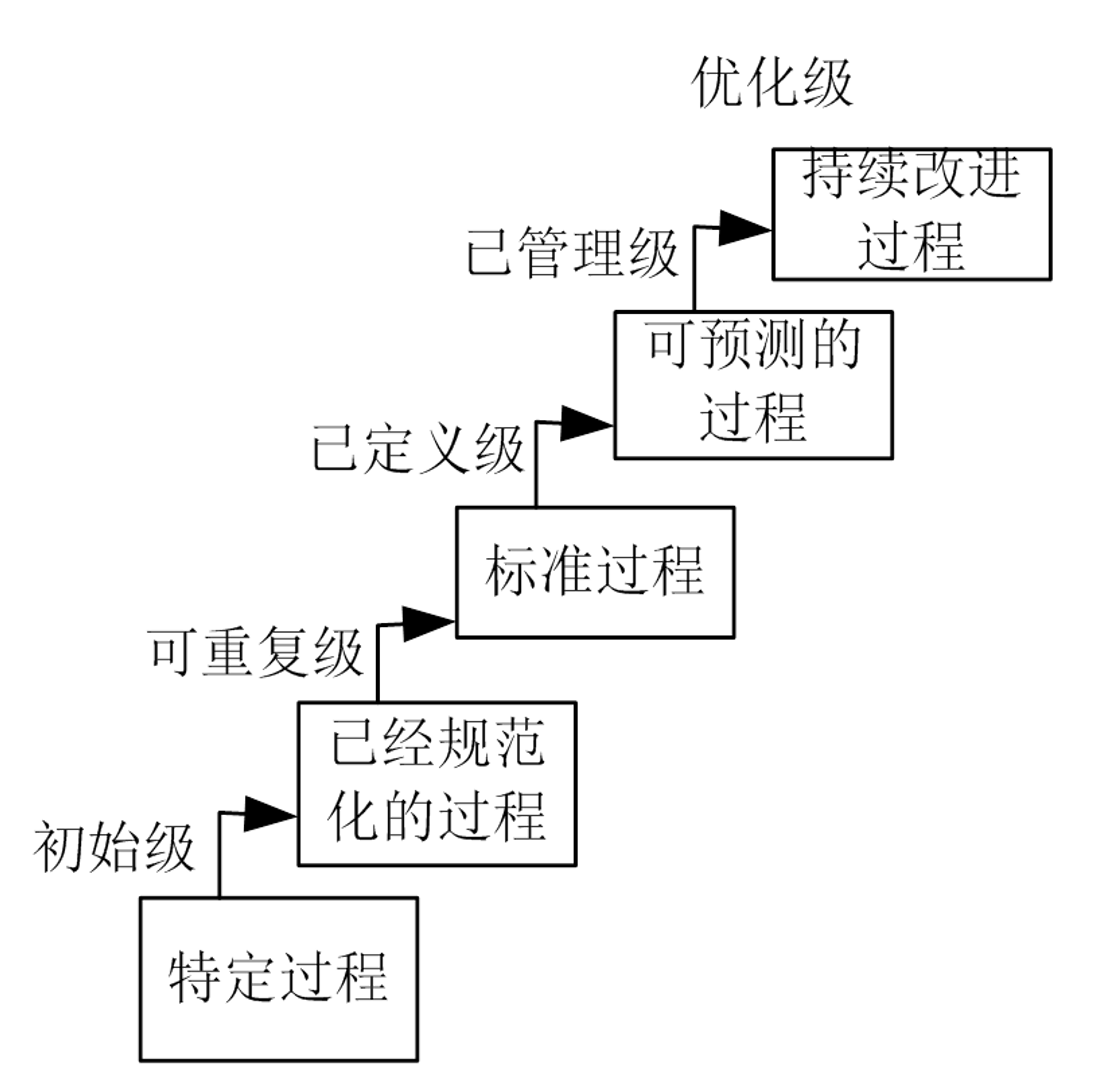
\includegraphics[width=\linewidth]{images/CMM1.png}
	\end{minipage}
	}
	\subfloat{
	\begin{minipage}[t]{0.56\linewidth}
	\centering
	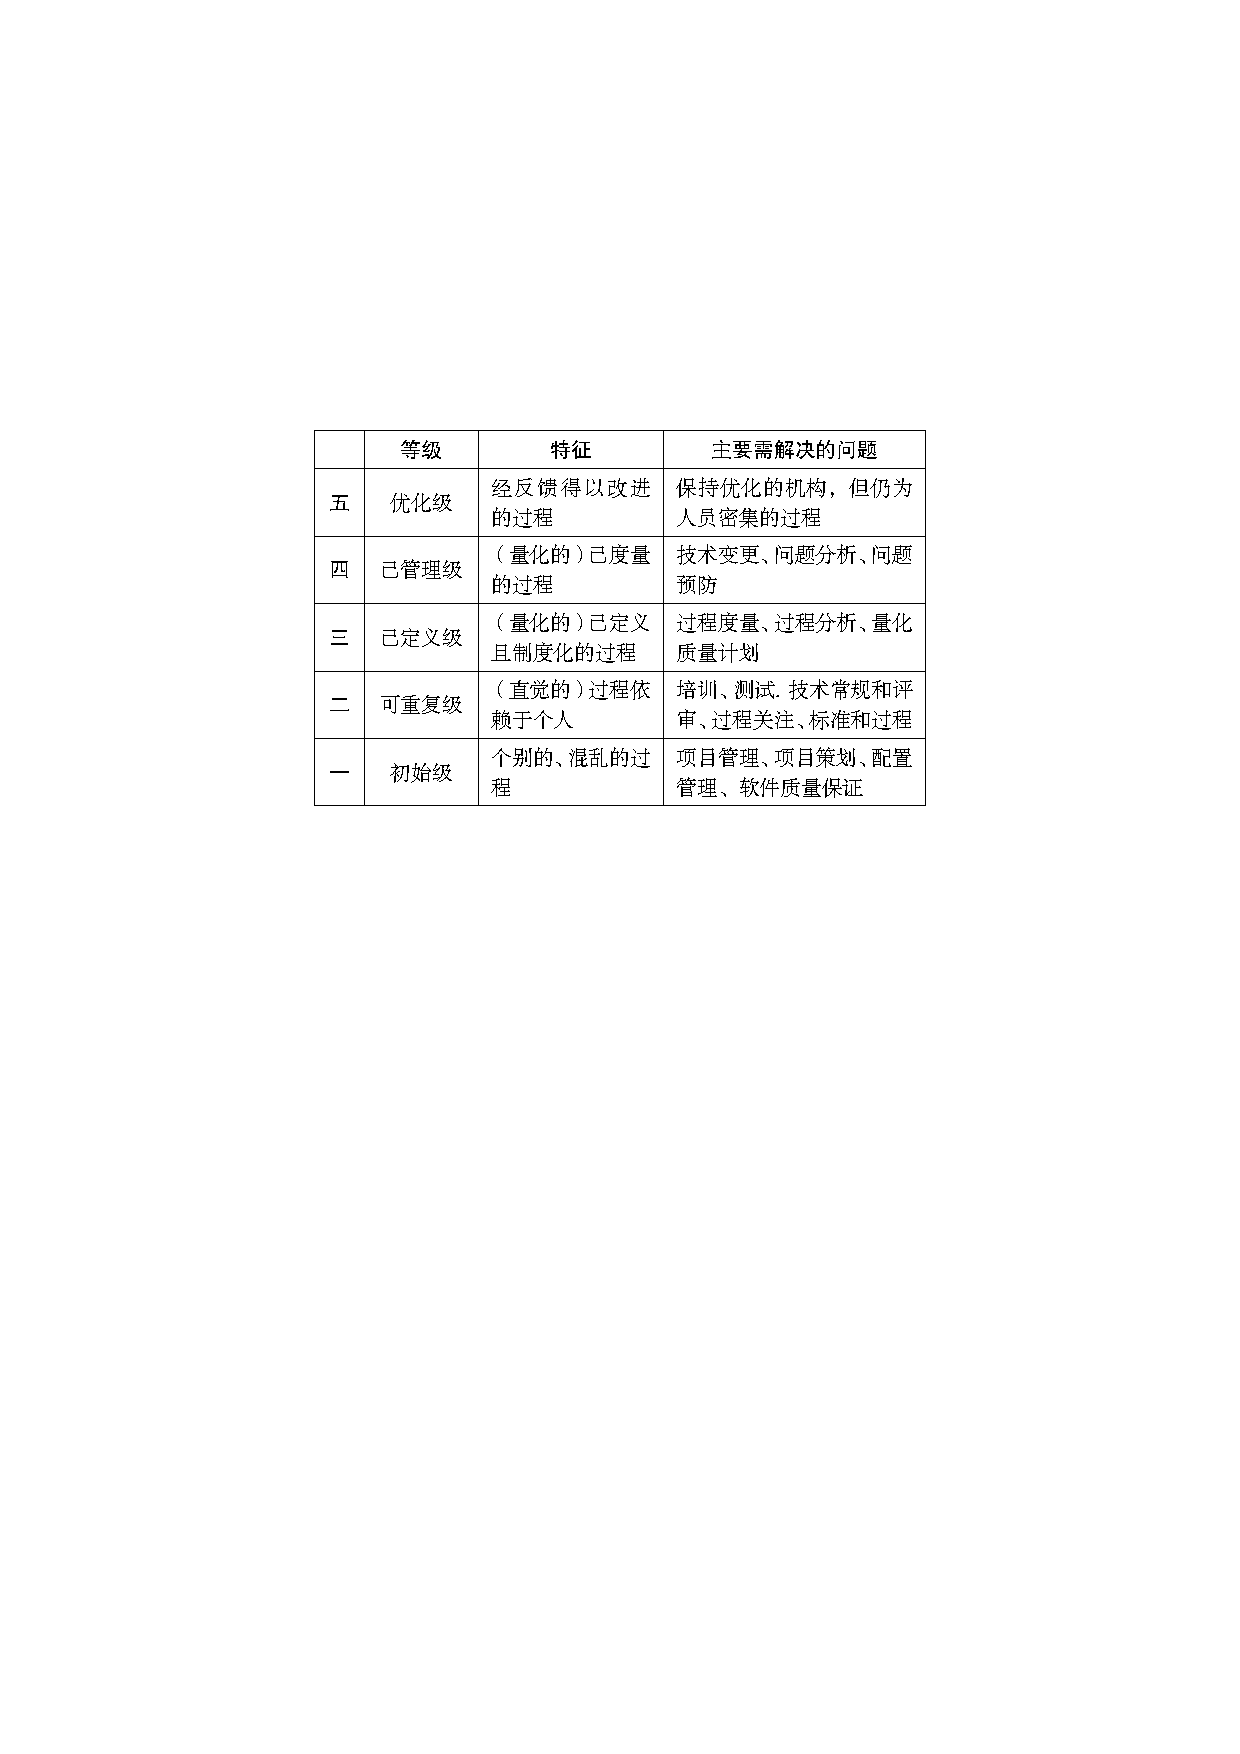
\includegraphics[width=\linewidth]{images/CMM2.pdf}
	\end{minipage}
	}
	\centering
\end{figure}


\subsubsection{考试题目}
\begin{problem}
	CMM的创始人是哪位?
	\uline{C}    
    \vspace{-0.8em}
    \begin{multicols}{4}
        \begin{enumerate}[label=\Alph*.]
            \item Boehm
            \item Juran
            \item Humphrey
            \item Crosby
        \end{enumerate}
    \end{multicols}
    \vspace{-1em}
\end{problem}


\subsection{软件过程管理/改进模型:CMMI}
CMMI (Capability Maturity Model Integration)能力成熟度集成模型
\begin{itemize}
    \item 刻画了软件团队/组织从不成熟到成熟的每个阶段的特征(也就是roadmap)
    \item 等级2和等级3关注的是当前状态
    \item 等级4和等级5是根据结果(未来)来进行管理
\end{itemize}

\subsubsection{等级一:初始级}
开发相对混乱,依赖个人英雄主义,没有过程概念,救火文化盛行
\begin{itemize}
    \item 软件组织对项目的目标与要做的努力很清晰,项目的目标可以实现
    \item 由于任务的完成带有很大的偶然性,软件组织无法保证在实施同类项目时仍然能够完成任务,项目实施是否成功主要取决于实施人员
\end{itemize}

\subsubsection{等级二:已管理级}
项目小组体现出项目管理的特征,有项目计划和跟踪、需求管理、配置管理等
\begin{itemize}
    \item 软件组织对项目有一系列管理程序,避免了软件组织完成任务的随机性,保证了软件组织实施项目的成功率
    \item 软件组织在项目实施上能够遵守既定的计划与流程,有资源准备,权责到人,对项目相关的实施人员进行相应的培训,对整个流程进行监测与控制,并联合上级单位对项目与流程进行审查
    \item 从2级升级到3级的原因:固化最佳实践,对小组而言是能够更快地学习其他的做法
\end{itemize}

\subsubsection{等级三:已定义级}
公司层面有标准流程和相应的规范,每个项目小组可以基于此定义自己的过程,使得优秀的做法可以在公司内分享
\begin{itemize}
    \item 软件组织能够根据自己的特殊情况及自己的标准流程,将这套管理体系与流程予以制度化
    \item 软件组织不仅能够在同类项目上成功,也可以在其他项目上成功
    \item 科学管理成为软件组织的一种文化,成为软件组织的财富
\end{itemize}

\subsubsection{等级四:定量管理级}
构建预测模型,以统计过程控制的手段来管理过程
\begin{itemize}
    \item 软件组织的项目管理实现了数字化
    \item 通过数字化技术来实现流程的稳定性,实现管理的精度,降低项目实施在质量上的波动
    \item 在这个级别我们希望能够看到一个预测模型
\end{itemize}

\subsubsection{等级五:优化级}
继续应用统计方法识别过程偏差,找到问题根源并消除,避免未来继续发生类似问题
\begin{itemize}
    \item 软件组织能够充分利用信息资料,对软件项目在项目实施的过程中可能出现的次品予以预防
    \item 能够主动地改善流程,运用新技术,实现流程的优化
\end{itemize}

\subsubsection{一些理解}
CMM/CMMI不适用于软件开发的原因
\begin{itemize}
    \item CMM/CMMI并不是一种具体的软件过程或者软件开发方法
    \begin{itemize}
        \item CMM/CMMI建立了一组有效地描述成熟软件组织特征的准则
        \item CMMI是过程改进模型而非软件过程或者软件过程模型:CMMI指导软件过程改进,不指导开发
        \item 按照CMM/CMMI模型的要求,一个软件组织应当定义使用本软件组织特点的软件过程,并且不断优化该过程,来更好地实现软件组织的商业目标
    \end{itemize}
    \item CMM/CMMI并不能作为检验软件过程优劣的标准:过程改进对不同企业的含义不一样,成熟度等级无法脱离企业环境直接横向比较
    \item CMM/CMMI与其他软件过程或者软件开发方法的比较是没有任何意义的
\end{itemize}

一些误解:
\begin{itemize}
    \item CMMI模型需要适当裁剪以适应公司的实际情况:需要裁剪的是公司内部定义的组织级开发流程和开发规范
    \item CMMI模型太重了,不适合互联网时代的轻量级开发:这个说法的错误之处在于,不一定是CMMI重或者轻,而是,CMMI根本就不是开发模型
    \item CMMI模型只适合大公司、大项目,不适合小项目:首先没人检验过;其次,项目的大小衡量本身也缺乏值得信赖的参考依据;最后,接受这种说法的人还是把CMMI当成是一种特殊的开发模型
    \item CMMI模型只适合需求不变或者很少变化的场合,不适合需求不确定,变化很多的场合:CMMI不是开发模型,与需求变化与否无关,谈不上适应或者不适应
\end{itemize}

{\kaishu CMMI不是过程优劣的标准,也不适合用作公司之间的能力比较:}正确,CMMI本身是有评级。(美国国防部订单招标要求企业至少达到CMMI的3级)。因为公司的能力需要绝对东西,也就是能力强,能力弱,而CMMI衡量的是相对的水平,CMMI仅仅关注在本公司的目标下的等级

更多讨论:试论CMM/CMMI不适合在当前软件开发当中应用的原因(\url{https://www.jianshu.com/p/b7407257eedb})

\subsubsection{考试题目}
\begin{problem}
请描述CMMI模型的5个等级的特征,并且解释为何CMMI模型不应该是敏捷方法的对立面。

五个等级的特征:
\begin{enumerate}[label=\arabic*.]
    \item Initial 原始级别:开发相对混乱,依赖个人英雄主义,没有过程概念,救火文化盛行
    \item Managed 已管理级别:项目小组体现出项目管理的特征,有项目计划和跟踪、需求管理、配置管理等
    \item Defined 已定义级别:公司层面有标准流程和相应的规范,每个项目小组可以基于此定义自己的过程,使得优秀的做法可以在公司共享。
    \item Quantitatively Managed 定量管理级别:构建预测模型,以统计过程控制的手段来管理过程
    \item Optimizing 优化级:继续应用统计方法识别过程偏差,找到问题根源并消除,避免未来继续发生类似问题
\end{enumerate}

原因解释:CMMI是过程管理/改进模型,刻画了软件组织从不成熟到成熟的路线图,而大部分敏捷方法都是开发方法,因此两者是完全不同性质的事物,将两者对立是不合适的

\begin{figure}[H]
    \vspace{-0.5em}
	\centering
	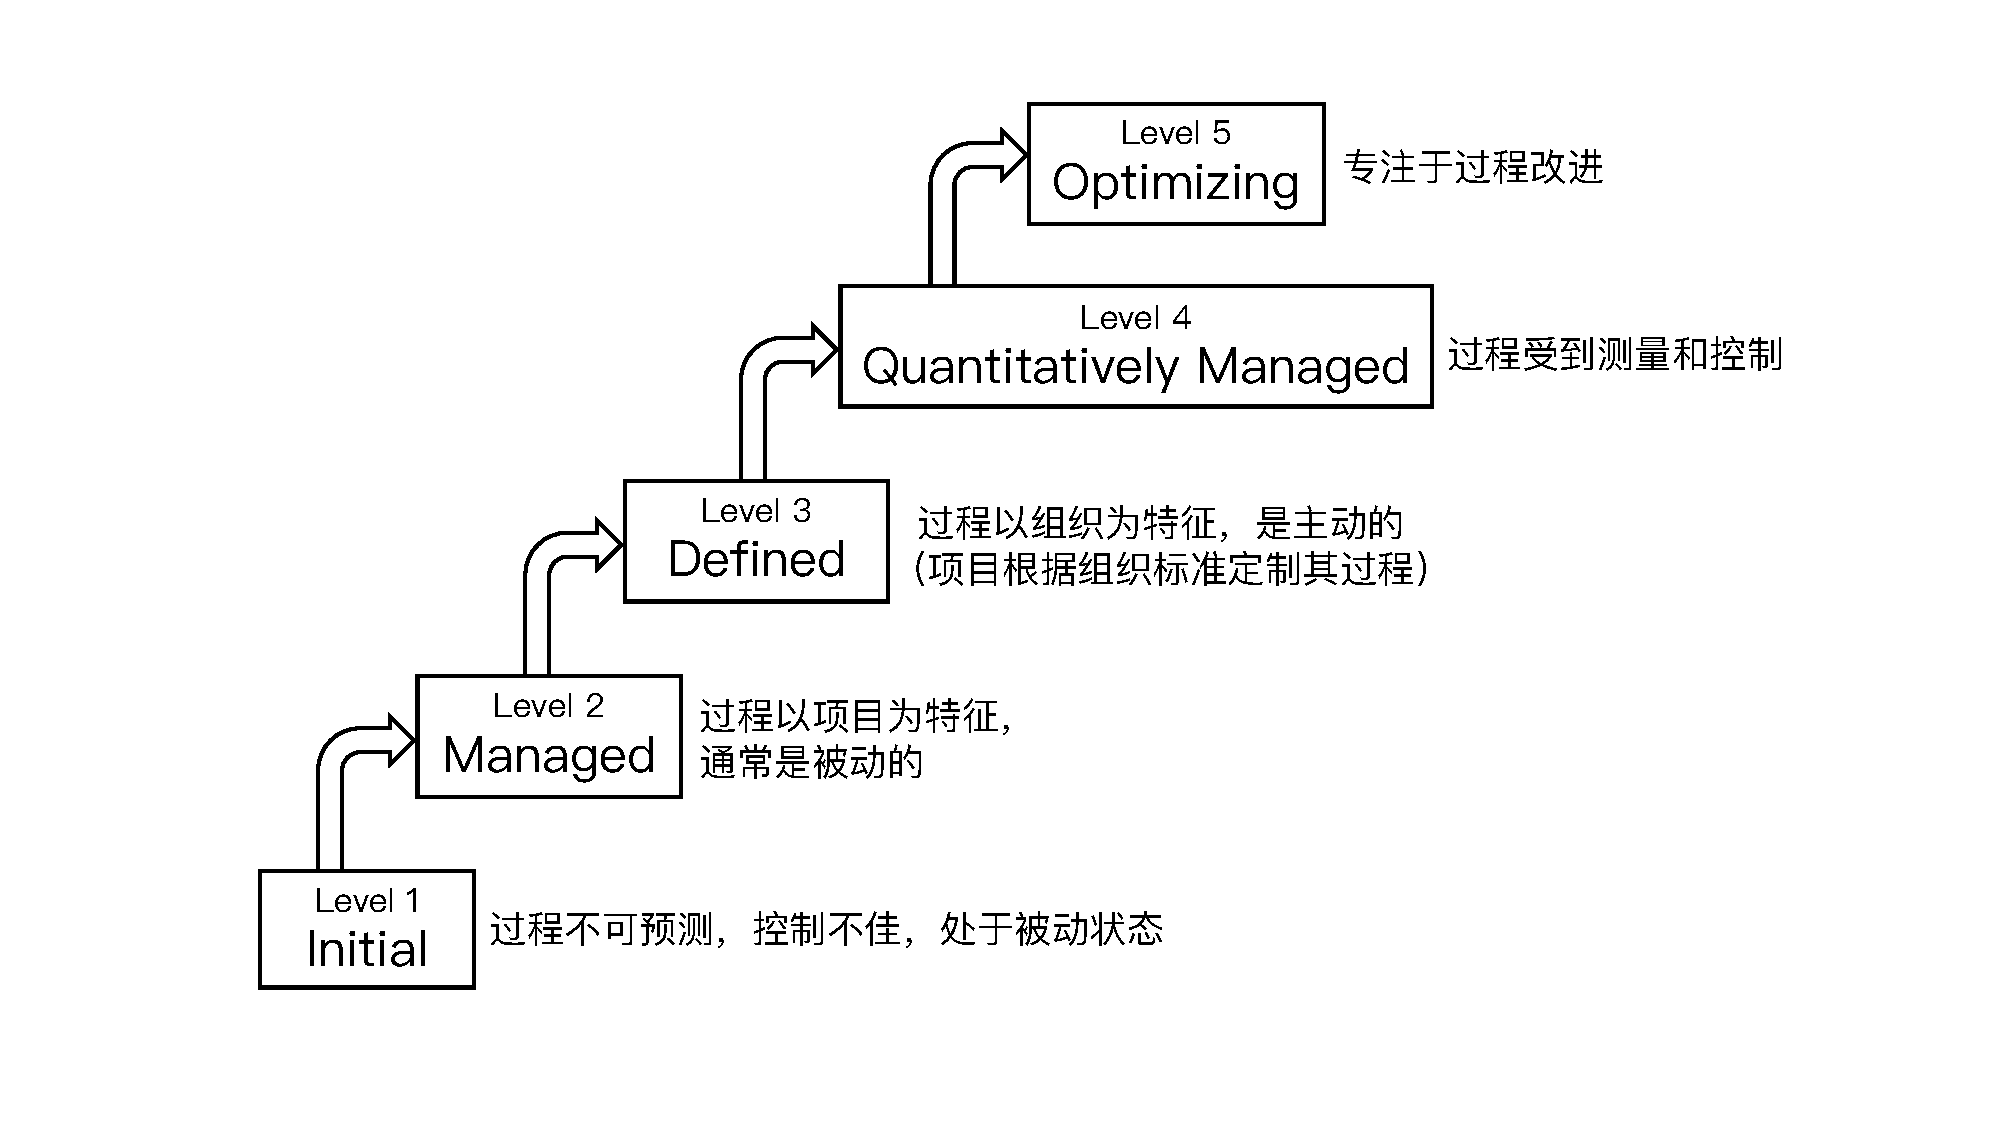
\includegraphics[width=0.65\textwidth]{images/CMMI.pdf}
    \vspace{-1em}
\end{figure}

\end{problem}


\subsection{软件过程改进模型:PDCA模型}
\begin{wraptable}{r}{6cm}
    \vspace{-4.5em}
	\centering
	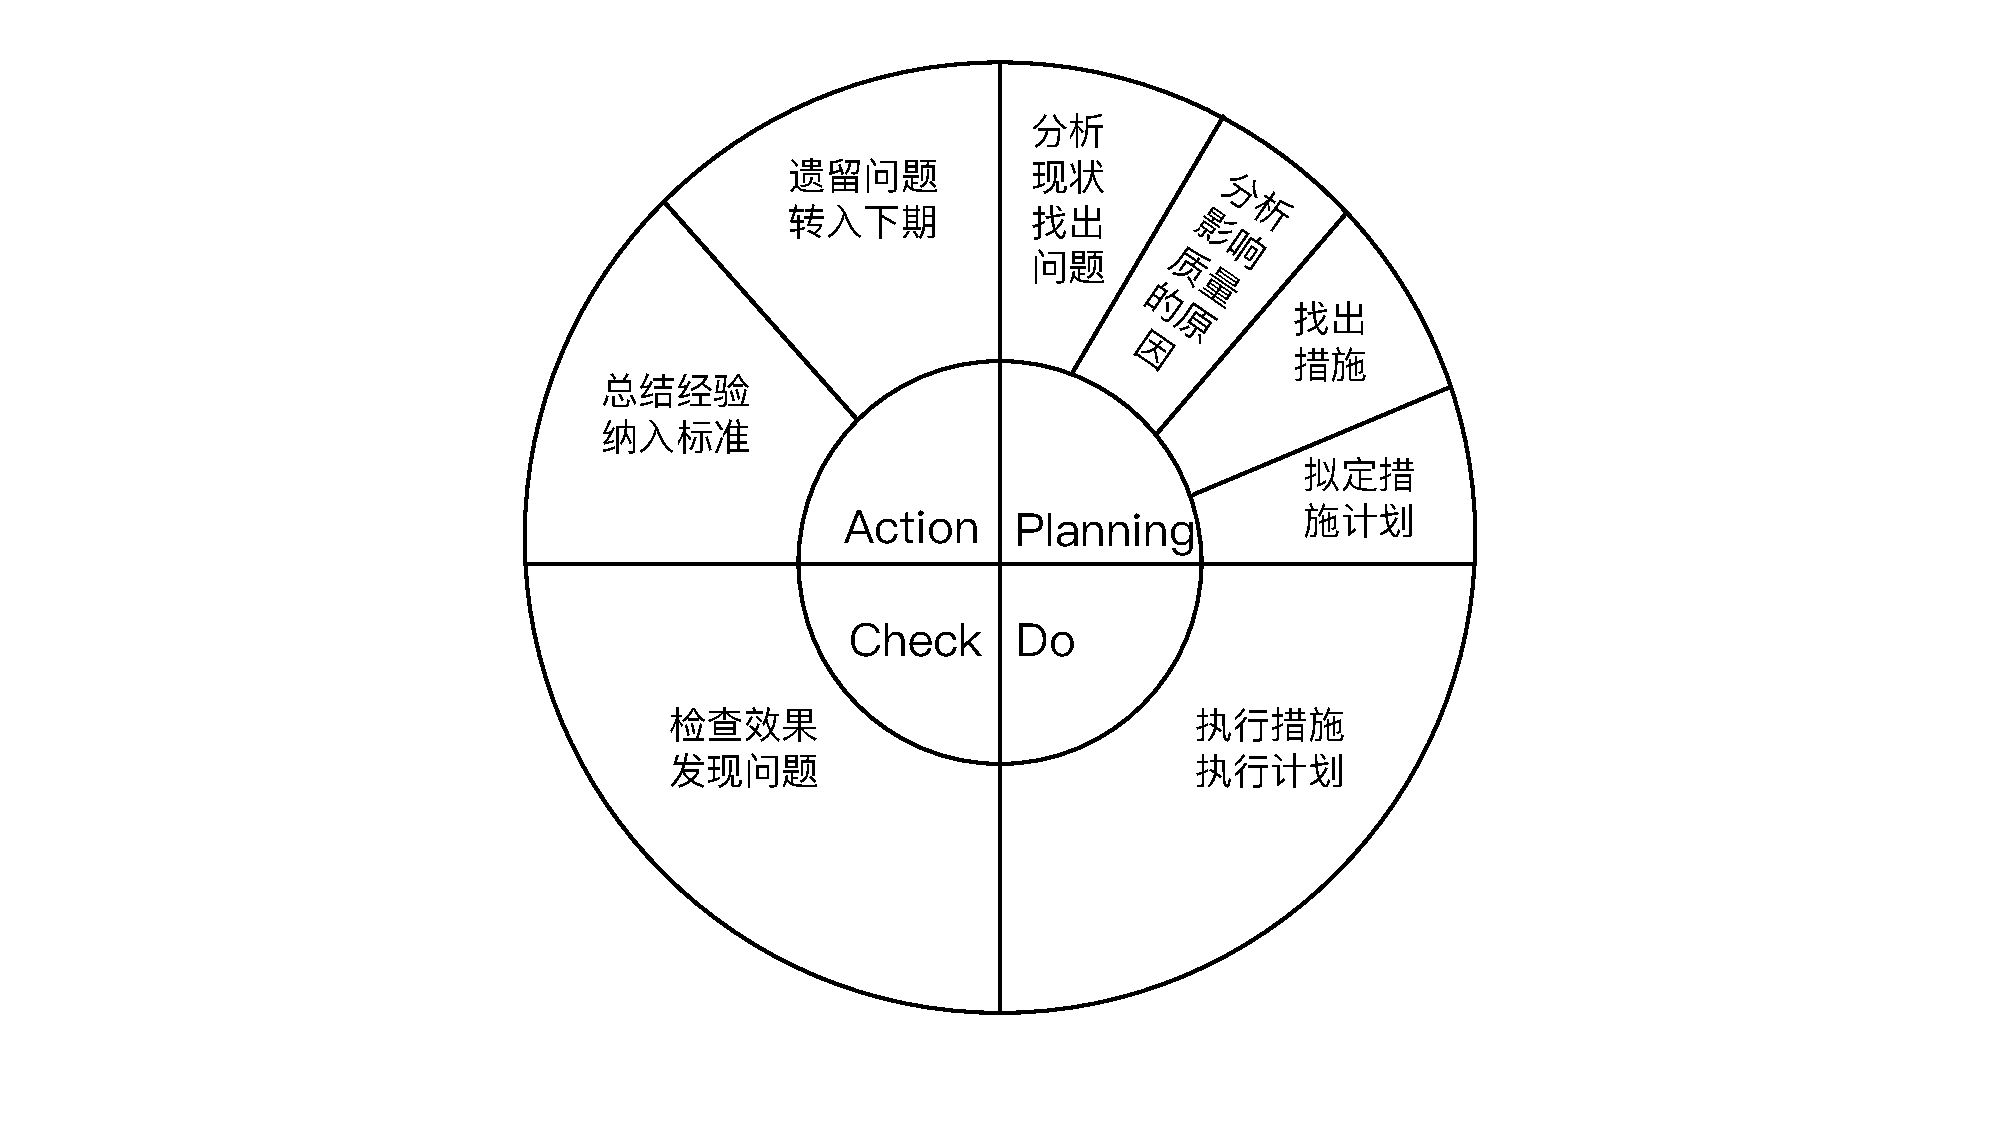
\includegraphics[width=0.4\textwidth]{images/PDCA.pdf}
    \vspace{-1em}
\end{wraptable}
PDCA模型的步骤:
\vspace{-0.8em}
\begin{multicols}{2}
    \begin{enumerate}[label=\arabic*.]
        \item 分析现状,找出问题
        \item 分析影响质量的原因
        \item 找出措施
        \item 拟定措施计划
        \item 执行措施,执行计划
        \item 检查效果,发现问题
        \item 总结经验,纳入标准
        \item 遗留问题转入下期PDCA循环
    \end{enumerate}
\end{multicols}
\vspace{-1em}

\subsubsection{考试题目}
\begin{problem}
请描述PDCA模型的主要步骤。
\end{problem}


\subsection{软件过程改进模型:IDEAL模型}
IDEAL模型解决了软件组织在各种质量改进环境下的需要。它包括了软件过程改进周期中的五个阶段,IDEAL是代表这五个阶段的单词的首字母
\vspace{-0.8em}
\begin{multicols}{3}
    \begin{itemize}
        \item I: Initiating 初始
        \item D: Diagnosing 诊断
        \item E: Establishing 建立
        \item A: Acting 执行
        \item L: Leveraging 调整
    \end{itemize}
\end{multicols}
\vspace{-1em}

\begin{figure}[H]
    \vspace{-0.5em}
	\centering
	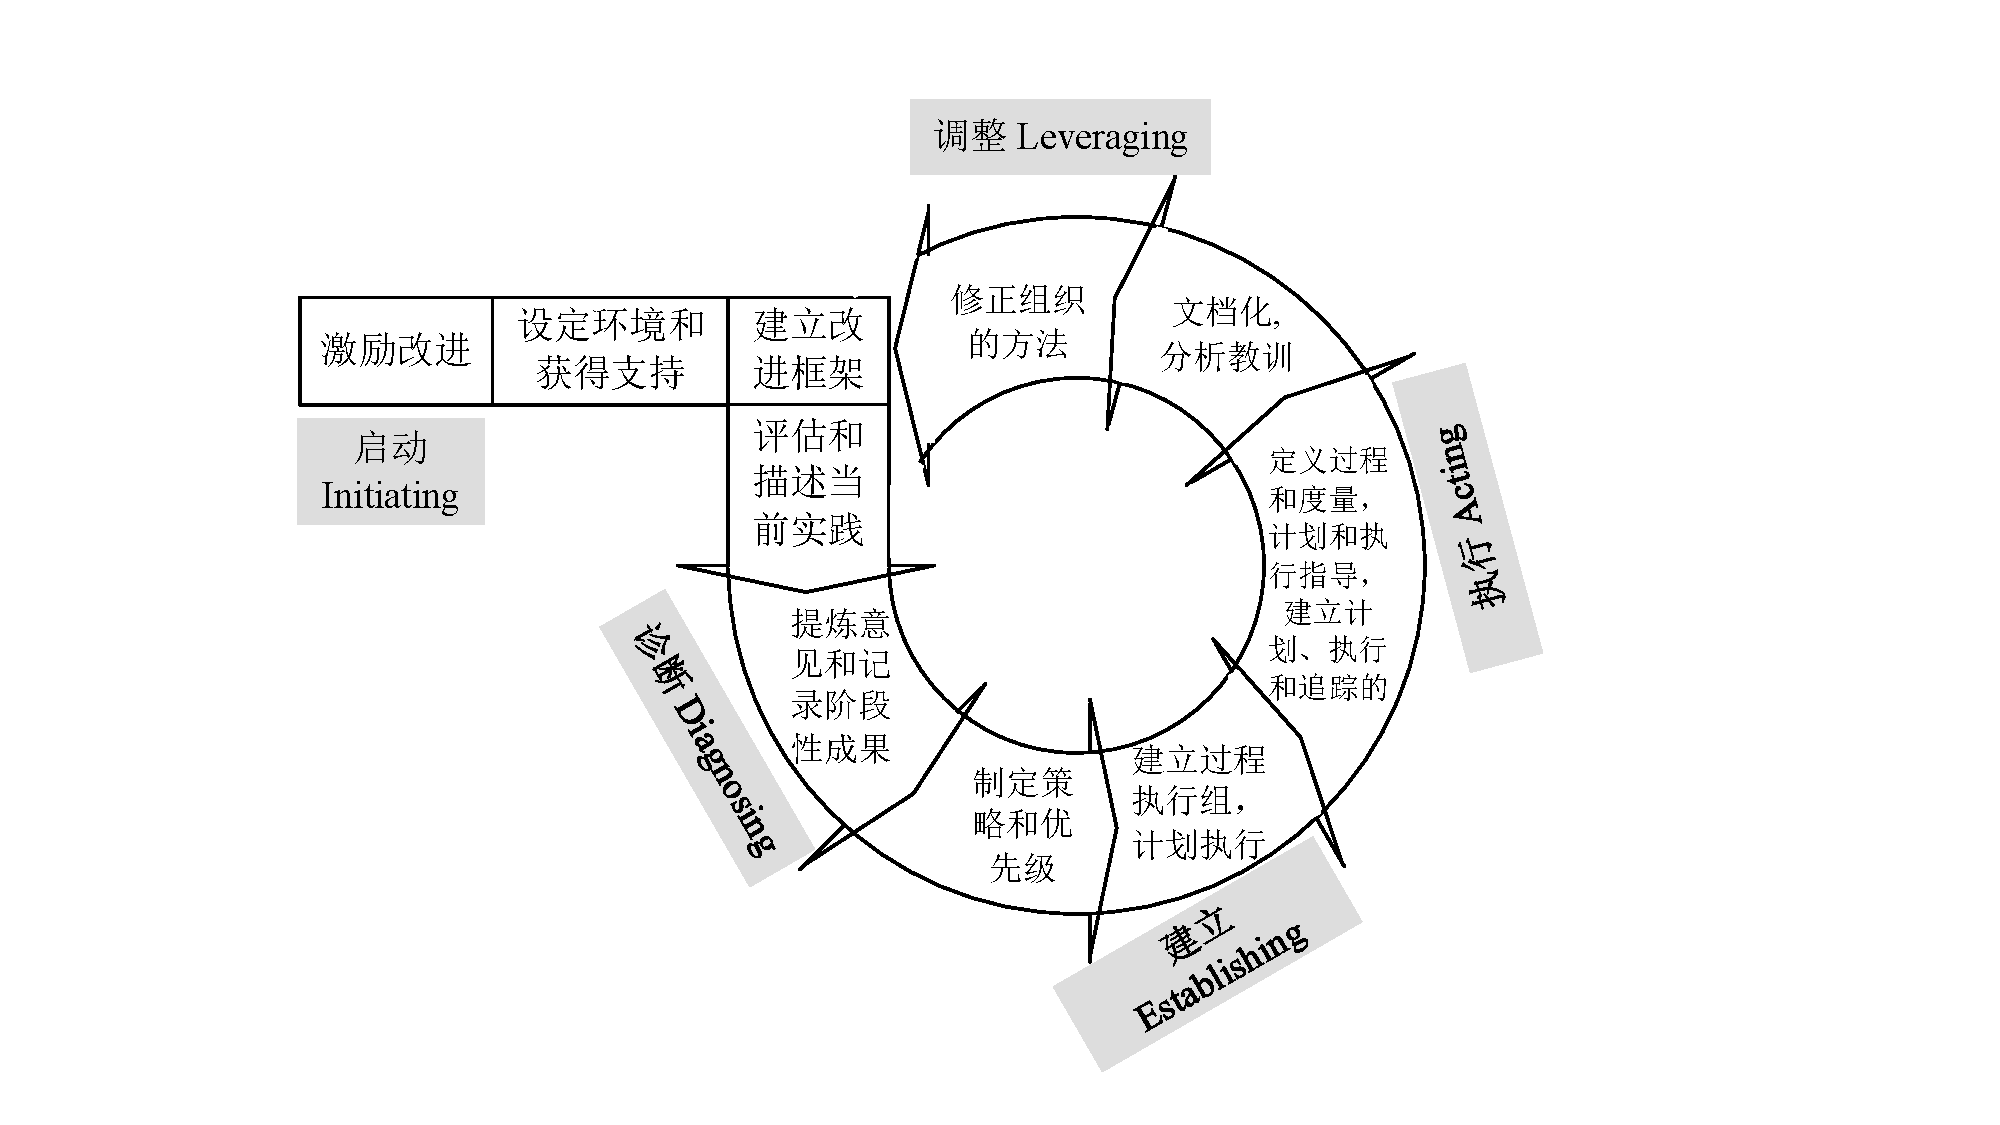
\includegraphics[width=0.63\textwidth]{images/IDEAL.pdf}
    \vspace{-1em}
\end{figure}


\subsection{软件过程管理模型:ISO/IEC 1504}
也叫SPICE (Software Process Improvement and Capability Determination),过程类别共有五种,分别是:
\vspace{-0.8em}
\begin{multicols}{3}
    \begin{itemize}
        \item 客户-供应商(CUS)过程
        \item 工程(ENG)过程
        \item 支持(SUP)过程
        \item 管理(MAN)过程
        \item 组织(ORG)过程
    \end{itemize}
\end{multicols}
\vspace{-1em}

重点关注“过程质量”,强调“持续改进”,获得ISO 9000标准认证的企业应该具有CMM第$2\sim 3$级的水平


\subsection{软件过程框架:RUP}
Rational统一过程(Rational Unified Process, RUP),它是由Rational软件公司推出的一种软件过程

RUP总结了经过多年商业化验证的6条最有效的软件开发经验,这些经验被称为“最佳实践”
\vspace{-0.8em}
\begin{multicols}{3}
    \begin{enumerate}[label=\arabic*.]
        \item 迭代式开发
        \item 管理需求
        \item 使用基于构件的体系结构
        \item 可视化建模
        \item 验证软件质量
        \item 控制软件变更
    \end{enumerate}
\end{multicols}
\vspace{-1em}

RUP软件开发生命周期:
\begin{enumerate}[label=\arabic*.]
    \item 初始阶段:建立业务模型,定义最终产品视图,并且确定项目的范围
    \item 精化阶段:设计并确定系统的体系结构,制定项目计划,确定资源需
    \item 构建阶段:开发出所有构件和应用程序,把它们集成为客户需要的产品,并且详尽地测试所有功能
    \item 移交阶段:把开发的产品提交给用户使用
\end{enumerate}

\subsection{软件质量管理发展}
\begin{problem}
描述下述质量管理大师的主要观点和贡献,工作对软件过程和项目管理的借鉴意义
\end{problem}

\subsubsection{Shewhart}
\begin{itemize}
    \item 最早将\textbf{统计控制}的思想引入质量管理,是质量改进奠基人
    \item 提出PDS模型(计划执行检查Plan-Do-See),后被戴明进一步发展为PDCA
\end{itemize}

\subsubsection{Deming}
\begin{itemize}
    \item \textbf{质量改进}:提出质量改进的思想,被称为日本质量管理之父
    \item \textbf{PDCA循环}:提出PDCA循环,被称为“\textbf{戴明环}”(Plan、Do、Check、Action),为最基本的质量和管理工具
\end{itemize}

\textbf{戴明管理14条原则:}
\vspace{-0.8em}
\begin{multicols}{2}
    \begin{enumerate}[label=\arabic*.]
        \item 树立改进产品和服务的坚定目标
        \item 采用新的思维方法
        \item 停止依赖检验的办法获得质量
        \item 不再凭价格标签进货
        \item 坚持不懈地提高产品质量和生产率
        \item 岗位培训制度化
        \item 管理者的作用应突出强调
        \item 排除畏难情绪
        \item 打破部门和人员之间的障碍
        \item 不再给操作人员提空洞的口号
        \item 取消对操作人员规定的工作定额和指标
        \item 不再采用按年度对人员工件进行评估
        \item 创建积极的自我提高计划制度
        \item 让每个员工都投入到提高产品质量的活动中去
    \end{enumerate}
\end{multicols}
\vspace{-1em}

\subsubsection{Juran}
\begin{itemize}
    \item 主编\textbf{质量控制手册}:《质量控制手册》为当今世界质量控制科学的“圣经”,奠定了“全面质量管理”TQM的理论基础(Total Quality Management)
    \item 提出\textbf{适用性质量}:
    \begin{itemize}
        \item 适用性质量:质量是一种适用性,即产品在使用期间能满足使用者的要求
        \item 质量不仅仅要满足明确的需求,还要满足潜在的需求。该思想使得质量管理范围从生产过程中的控制进一步扩大到产品开发和工艺设计阶段,即挖掘用户潜在需求
    \end{itemize}
    \item 提出\textbf{质量三步曲}:就是质量计划$\rightarrow$质量控制$\rightarrow$质量改进
    \item 提出\textbf{Juran质量螺旋}
    \item 提出\textbf{80/20原则}:认为有80\%的质量问题是由领导责任引起的,从而将人力与质量管理结合起来
\end{itemize}

\subsubsection{Crosby}
\begin{itemize}
    \item 提出\textbf{零缺陷}的概念:
    \begin{itemize}
        \item 零缺陷:第一次就把事情做对。想要做到这一点,就需要把工作放在预防上而不是质量检验上
    \end{itemize}
    \item 提出\textbf{质量管理}的绝对性:
    \vspace{-0.8em}
    \begin{multicols}{2}
        \begin{itemize}
            \item 质量就是符合要求,而不是“完美”
            \item 质量来自于预防,而不是检验
            \item 质量的标准是“零缺陷”,而不是可接受质量水平
            \item 质量的衡量标准是“不符合要求的代价”
        \end{itemize}
    \end{multicols}
    \vspace{-1em}
    \item 提出质量改进的基本要素(6C-变革管理的六个阶段):
    \vspace{-0.8em}
    \begin{multicols}{2}
        \begin{itemize}
            \item 领悟(Comprehension):理解质量真谛
            \item 承诺(commitment):制定质量策略的决心
            \item 能力(capability):教育与培训
            \item 沟通(communication):成功的经验文档化、制度化
            \item 改正(correction):预防与提高绩效
            \item 坚持(continuance):强调质量管理成为一种工作方式
        \end{itemize}
    \end{multicols}
    \vspace{-1em}
    \item 发展质量成熟度的度量
\end{itemize}


\subsubsection{Humphrey 软件过程之父}
\begin{itemize}
    \item 采用Crosby的成熟度度量,提出了软件能力成熟度模型(CMM) ,对于软件过程管理与改进具有建设性作用
    \item 将上述的理论和实践引入软件过程
\end{itemize}


	\section{敏捷软件开发}
敏捷中也有计划驱动

\subsection{敏捷目的}
为了使软件开发团队具有高效工作和快速响应变化的能力

\subsection{敏捷原则}
\vspace{-0.8em}
\begin{multicols}{2}
    \begin{enumerate}[label=\arabic*.]
        \item 最重要的是通过尽早和不断交付有价值的软件满足客户需要
        \item 欢迎需求的变化
        \item 经常交付可以工作的软件,从几星期到几个月,时间尺度越短越好
        \item 业务人员和开发者应该在整个项目过程中始终朝夕在一起工作
        \item 最好的信息传达方式是面对面的交谈
    \end{enumerate}
\end{multicols}
\vspace{-1em}


\subsection{敏捷宣言}
\vspace{-0.8em}
\begin{multicols}{2}
    \begin{itemize}
        \item 个体和互动 胜过 流程和工具
        \item 可以工作的软件 胜过 详尽的文档
        \item 客户合作 胜过 合同谈判
        \item 响应变化 胜过 遵循计划
    \end{itemize}
\end{multicols}
\vspace{-1em}
\vspace{-0.4em}
\begin{itemize}
    \item 也就是说,尽管右项有其价值,我们更重视左项的价值
\end{itemize}

\begin{problem}
请完整描述敏捷宣言。
\end{problem}

\subsection{敏捷软件开发方法}
\subsubsection{极限编程 XP}
eXtreme Programming,极限的含义是指把好的开发实践运用到极致

极限编程的有效实践
\vspace{-0.8em}
\begin{multicols}{2}
    \begin{itemize}
        \item 客户作为开发团队的成员——客户代表
        \item 使用用户素材
        \item 短交付周期
        \item 验收测试
        \item 结对编程——结对编程就是由两名开发人员在同一台计算机上共同编写解决同一个问题的程序代码,通常一个人编码,另一个人对代码进行审查与测试,以保证代码的正确性与可读性。结对编程是加强开发人员相互沟通与评审的一种方式
        \item 测试驱动开发——极限编程强调“测试先行”。在编码之前,应该首先设计好测试方案,然后再编程,直至所有测试都获得通过之后才可以结束工作
        \item 集体所有
        \item 持续集成
        \item 可持续的开发速度 $\leq$40h/week
        \item 开放的工作空间
        \item 重构
        \item 使用隐喻
    \end{itemize}
\end{multicols}
\vspace{-1em}

\subsubsection{Scrum}
迭代式增量软件开发过程:
\begin{figure}[H]
    \vspace{-0.5em}
	\centering
	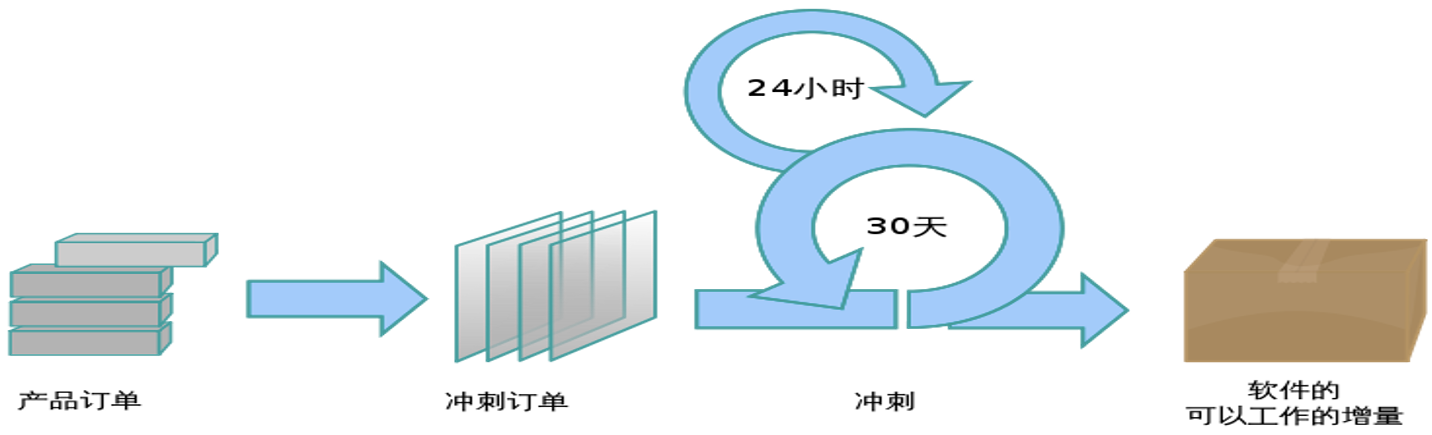
\includegraphics[width=0.65\textwidth]{images/Scrum.png}
    \vspace{-1em}
\end{figure}

Scrum中的文档:
\begin{itemize}
    \item 产品订单(product backlog):整个项目的概要文档,包含了已划分优先等级的、项目要开发的系统或产品的需求清单,是动态的
    \item 冲刺订单(sprint backlog):细化了的文档,包含了团队如何实现下一个冲刺的需求信息
    \begin{itemize}
        \item 哪些产品订单会加入一次冲刺由冲刺计划会议决定。会议中,产品负责人告诉开发团队他们需要完成产品订单中的哪些订单项,开发团队决定在下一次冲刺中承诺完成多少订单项
        \item 在冲刺的过程中,没有人能够变更冲刺订单,这意味着在一个冲刺中需求是被冻结的
    \end{itemize}
    \item 燃尽图(burn down chart)
\end{itemize}

Scrum中角色:
\begin{itemize}
    \item 产品负责人,代表利益所有者
    \begin{itemize}
        \item 产品负责人的职责是将开发团队开发的产品价值最大化
        \item 产品负责人是负责管理产品待办列表的唯一负责人。产品待办列表的管理包括:
        \begin{itemize}
            \item 清晰地表述产品待办列表项
            \item 对产品待办列表项进行排序,使其最好地实现目标和使命
            \item 优化开发团队所执行工作的价值
            \item 确保产品待办列表对所有人是可见、透明和清晰的,同时显示 Scrum 团队下一步要做的工作
            \item 确保开发团队对产品待办列表项有足够深的了解
        \end{itemize}
    \end{itemize}
    \item Scrum Master, 类似于项目经理,负责维护过程和任务
    \begin{itemize}
        \item 促进和支持 SCRUM
        \item 帮助每个人理解 SCRUM 理论、实践、规则和价值
        \item SCRUM Master 是一位服务型领导
        \begin{itemize}
            \item 帮助 SCRUM 团队之外的人了解如何与 SCRUM 团队交互是有益的
            \item 改变SCRUM 团队之外的人与 SCRUM 团队的互动方式来最大化 SCRUM 团队所创造的价值
        \end{itemize}
        \item Scrum Master 服务于产品负责人,包括:
        \begin{itemize}
            \item 确保 Scrum 团队中的每个人都尽可能地理解目标、范围和产品域
            \item 找到有效管理产品待办列表的技巧
            \item 帮助 Scrum 团队理解为何需要清晰且简明的产品待办列表项
            \item 理解在经验主义的环境中的产品规划
            \item 确保产品负责人懂得如何来安排产品待办列表使其达到最大化价值
            \item 理解并实践敏捷性
            \item 当被请求或需要时,引导 Scrum 事件
        \end{itemize}
        \item Scrum Master 以各种方式服务于开发团队,包括:
        \begin{itemize}
            \item 作为教练在自组织和跨职能方面给予开发团队以指导
            \item 帮助开发团队创造高价值的产品
            \item 移除开发团队工作进展中的障碍
            \item 按被请求或需要时,引导 Scrum 事件
            \item 在 Scrum 还未完全采纳和理解的组织环境中,作为教练指导开发团队
        \end{itemize}
        \item Scrum Master 以各种方式服务于组织,包括:
        \begin{itemize}
            \item 带领并作为教练指导组织采纳 Scrum
            \item 在组织范围内规划 Scrum 的实施
            \item 帮助员工和利益攸关者理解并实施 Scrum 和经验导向的产品开发
            \item 引发能够提升 Scrum 团队生产率的改变
            \item 与其他 Scrum Master 一起工作,增强组织中 Scrum 应用的有效性
        \end{itemize}
    \end{itemize}
    \item 开发团队
    \begin{itemize}
        \item 负责在每个 Sprint 结束时交付潜在可发布并且“完成”的产品增量。
        \item 开发团队由组织组建并得到授权,团队自己组织和管理他们的工作。开发团队具有下列特点:
        \begin{itemize}
            \item 他们是自组织的。没有人(即使是 Scrum Master)有权告诉开发团队应该如何把产品待办列表变成潜在可发布的功能增量
            \item 开发团队是跨职能的团队,团队作为一个整体,拥有创建产品增量所需的全部技能
            \item Scrum 不认可开发团队成员的任何头衔,不管其承担何种工作(他们都叫开发人员)
            \item Scrum 不认可开发团队中所谓的“子团队”,无论其需要处理的领域是诸如测试、架构、运维或业务分析
            \item 开发团队中的每个成员也许有特长和专注的领域,但是责任属于整个开发团队
        \end{itemize}
    \end{itemize}
\end{itemize}

Scrum常见活动
\vspace{-0.8em}
\begin{multicols}{3}
    \begin{enumerate}[label=\arabic*.]
        \item Sprint Planning Meeting
        \item Daily standup meeting
        \item review meeting
        \item retrospective meeting
        \item sprint
    \end{enumerate}
\end{multicols}
\vspace{-1em}

Empirical Process Control VS. Statistical Process Control,不同于统计过程控制方法(也叫预测式、计划式)不能解决不可预见的需求变化问题,Scrum采用的实证过程控制承认问题无法完全理解或定义,即用户可以在项目过程中变更需求,关注于如何使开发团队\textbf{快速推出和响应需求变化的能力}最大化


Scrum VS. XP
\begin{itemize}
    \item 迭代周期不同。XP迭代周期为$1\sim 2$周,而Scrum迭代周期为$2\sim 4$周
    \item 迭代中是否允许需求变更。XP中只要变更需求与原需求所需时间资源相等即可变更,而Scrum在迭代中需求被冻结
    \item 迭代中,需求是否严格按照优先级来实现。XP中务必遵守优先级别,Scrum中则比较灵活,原因是可能有需求依赖问题
    \item 过程工程化。Scrum开发过程并未工程化,要求开发者自觉保证,但XP则对开发流程定义严格,例如TDD,结对编程,重构等
\end{itemize}

\subsubsection{Kanban方法}
\vspace{-0.8em}
\begin{multicols}{2}
    \begin{itemize}
        \item 精益生产(丰田制造法)的具体实现
        \item 可视化工作流、限定WIP、管理周期时间
        \item 马丁提出了微服务架构
    \end{itemize}
\end{multicols}
\vspace{-1em}

\subsection{考试题目}
\begin{problem}
	XP规定开发人员每周工作时间不超过\uline{\ \ \ \ \ \ }小时,连续加班不可以超过两周,以免降低生产率?
	\uline{B}    
    \vspace{-0.8em}
    \begin{multicols}{4}
        \begin{enumerate}[label=\Alph*.]
            \item 30
            \item 40
            \item 50
            \item 60
        \end{enumerate}
    \end{multicols}
    \vspace{-1em}
\end{problem}

\begin{problem}
	下列不属于看板方法典型实践的是?
	\uline{BD}    
    \vspace{-0.8em}
    \begin{multicols}{4}
        \begin{enumerate}[label=\Alph*.]
            \item 可视化工作流
            \item 站立式会议
            \item 限定 WIP
            \item 重构
        \end{enumerate}
    \end{multicols}
    \vspace{-1em}
\end{problem}

\begin{problem}
请结合SCRUM这种敏捷方法论述敏捷方法应该具备的特征?同时解释为何常见的若干种描述敏捷方法对立面的方法的特征(例如,严格、重型、计划驱动等等)并不合适?

特征:1. 小周期迭代;2. 快速响应变更;3. 价值交付;4.自动化

特征解释:
\begin{enumerate}[label=\arabic*.]
    \item 严格:所有优秀的工程方法和实践都是严格的
    \item 重型:如上,此外,轻量级和重型其实并没有刻画具体方法,何为重型,并没有严格定义;而且,对于变更这件事情,几乎所有方法都是限制,因此,很难说敏捷方法是轻量级方法
    \item 计划驱动:所有正式的项目都是计划驱动的,否则计划的作用无法体现
\end{enumerate}
\end{problem}

\begin{problem}
敏捷方法的特征有哪些?哪些关于敏捷特征的说法施加于敏捷方法之上是不合适的?为什么?

特征:小周期迭代式、持续交付、敏捷宣言

关于敏捷方法的一些特征表述可能带着一定的误导,例如:
\begin{enumerate}[label=\arabic*.]
    \item 轻量级方法:这是对以XP为代表的一类方法的误导,事实上,这类方法对工程规范有着极为严格的要求
    \item 拥抱变更、变更驱动:仅仅是口号,对待变更,所有软件工程方法都是限制和管理的态度
    \item TDD(测试驱动开发)可以提供更高的开发质量:并没有足够的证据支持
\end{enumerate}
\end{problem}

\begin{problem}
为何说将“规范方法”、“计划驱动方法”等特征作为敏捷方法的对立面带有很大的误导性质?如何通过多种维度改进这种对各类开发过程的理解?

敏捷:敏捷目的、敏捷价值观、敏捷原则

影响敏捷与规范方法选择的五个维度
\begin{enumerate}[label=\arabic*.]
    \item 如果只有强有力的规范而缺乏敏捷,将导致官僚作风,进而停滞不前。团队将陷入为了测量而测量的处境之中,缺乏创新
    \item 缺乏创新的敏捷则如同一个新创公司在盈利之前的不负责任的狂热
    \item 计划驱动的开发人员必须敏捷,敏捷开发人员必须规范
\end{enumerate}
\end{problem}

\begin{problem}
Devops三个步骤
\end{problem}

\begin{problem}
Devops的特点,为什么流行?
\end{problem}

\begin{problem}
什么是云原生?相关的重要的概念
\end{problem}

\begin{problem}
精益屋的两大支柱?
\end{problem}

\begin{problem}
JIT及时生产,价值流和价值拉动的关系
\end{problem}

\begin{problem}
概念解释
\vspace{-0.8em}
\begin{multicols}{3}
    \begin{enumerate}[label=\arabic*.]
        \item CI
        \item CI/CD
        \item Pipeline Orchestration
        \item Container
        \item Micro Service
        \item A/B Testing
        \item GitFlow
    \end{enumerate}
\end{multicols}
\vspace{-1em}
\end{problem}

\begin{problem}
描述用途
\vspace{-0.8em}
\begin{multicols}{5}
    \begin{enumerate}[label=\arabic*.]
        \item Docker
        \item Jenkins
        \item JIRA
        \item SonarQube
        \item Git
    \end{enumerate}
\end{multicols}
\vspace{-1em}
\end{problem}
	\section{PSP个体软件过程}

\begin{figure}[H]
    \vspace{-0.5em}
	\centering
	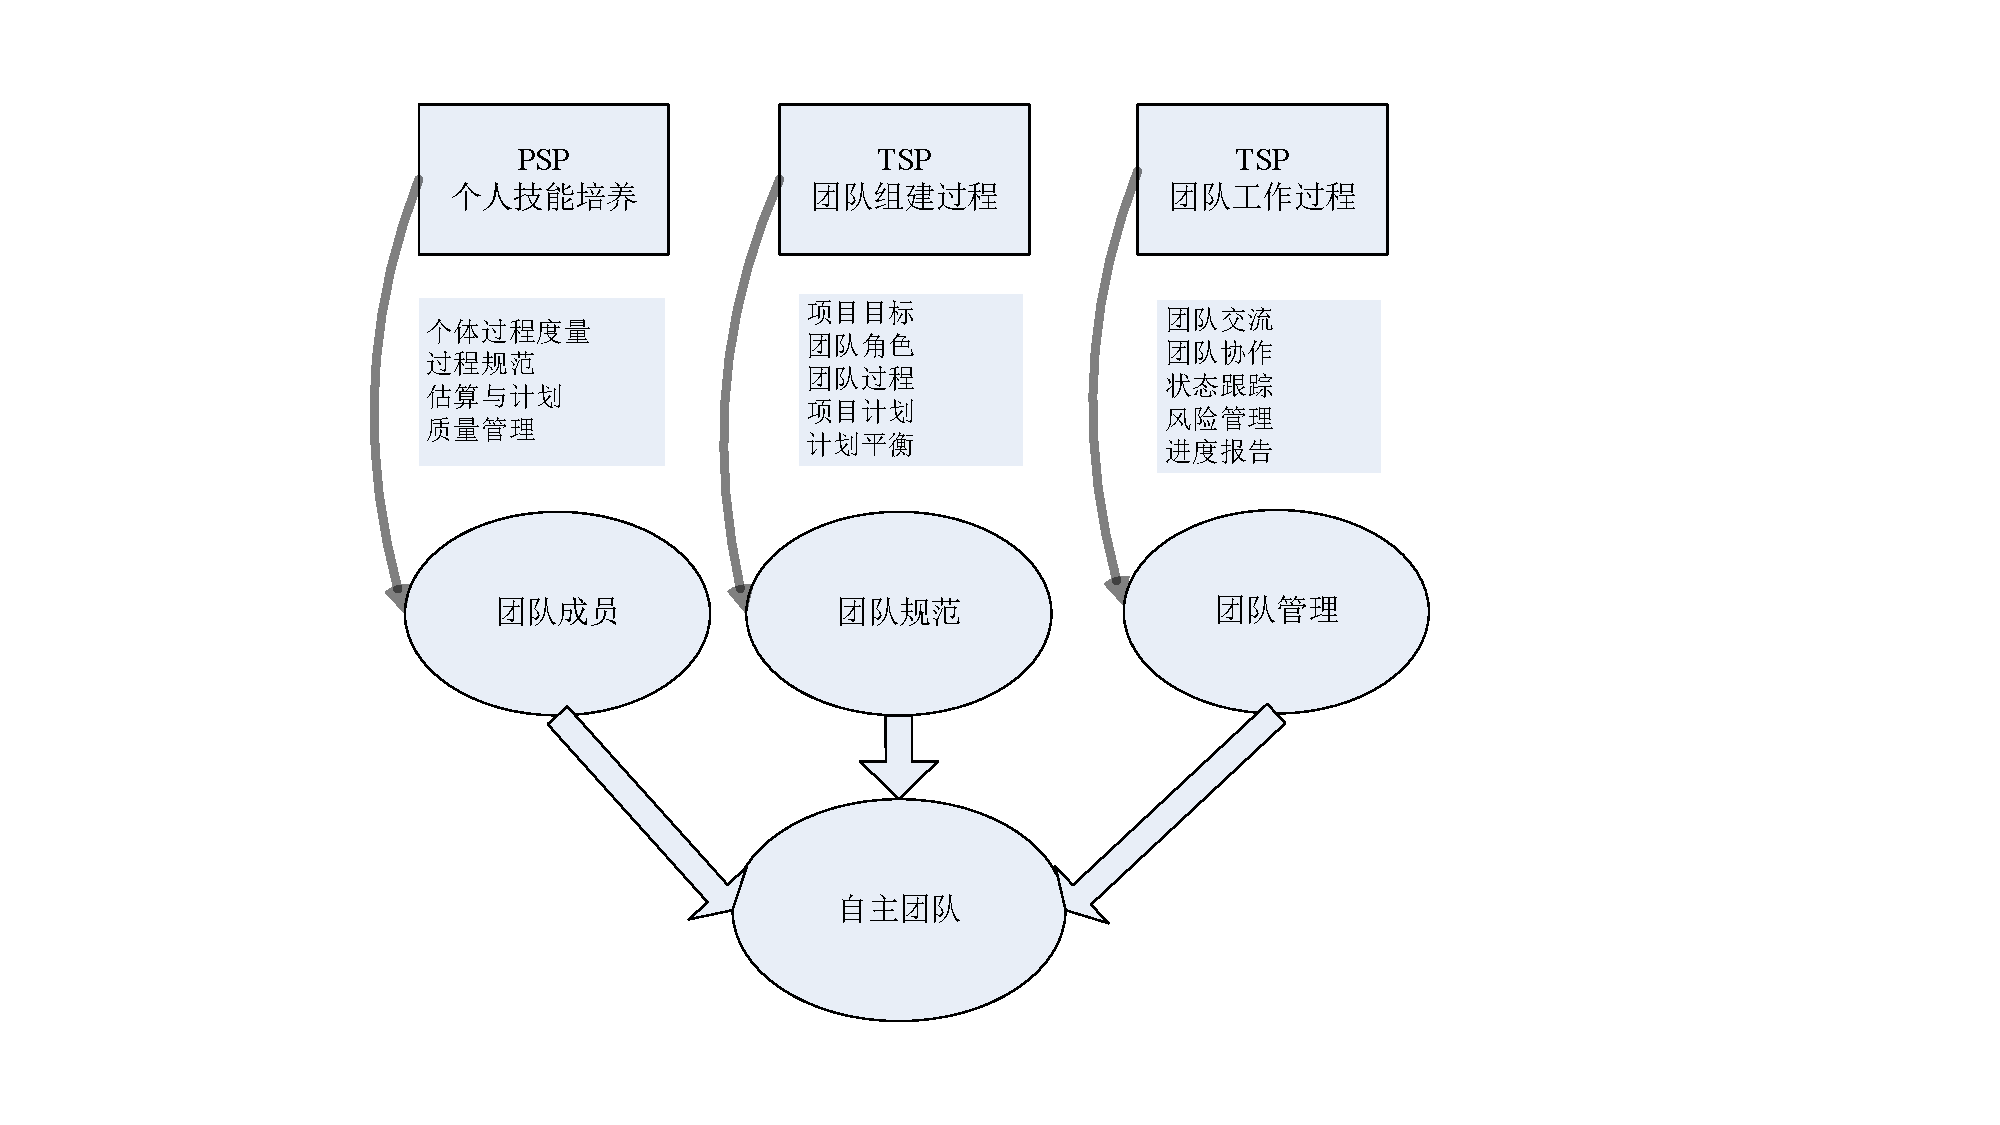
\includegraphics[width=0.7\textwidth]{images/PSP.pdf}
    \vspace{-1em}
\end{figure}

\subsection{PSP简介}
PSP是包括了数据记录表格、过程操作指南和规程在内的结构化框架

PSP着重于软件开发人员的个人能力提升,体现在估算能力、计划能力、计划执行以及质量管理等方面

基本的PSP包括策划、设计、编码、编译、单元测试以及总结等阶段
\begin{itemize}
    \item 每个阶段,都有相应的过程操作指南,用来指导该阶段的开发活动。
    \item 所有的开发活动都需要记录相应的时间日志和缺陷日志
\end{itemize}

\begin{figure}[H]
    \vspace{-0.5em}
	\centering
	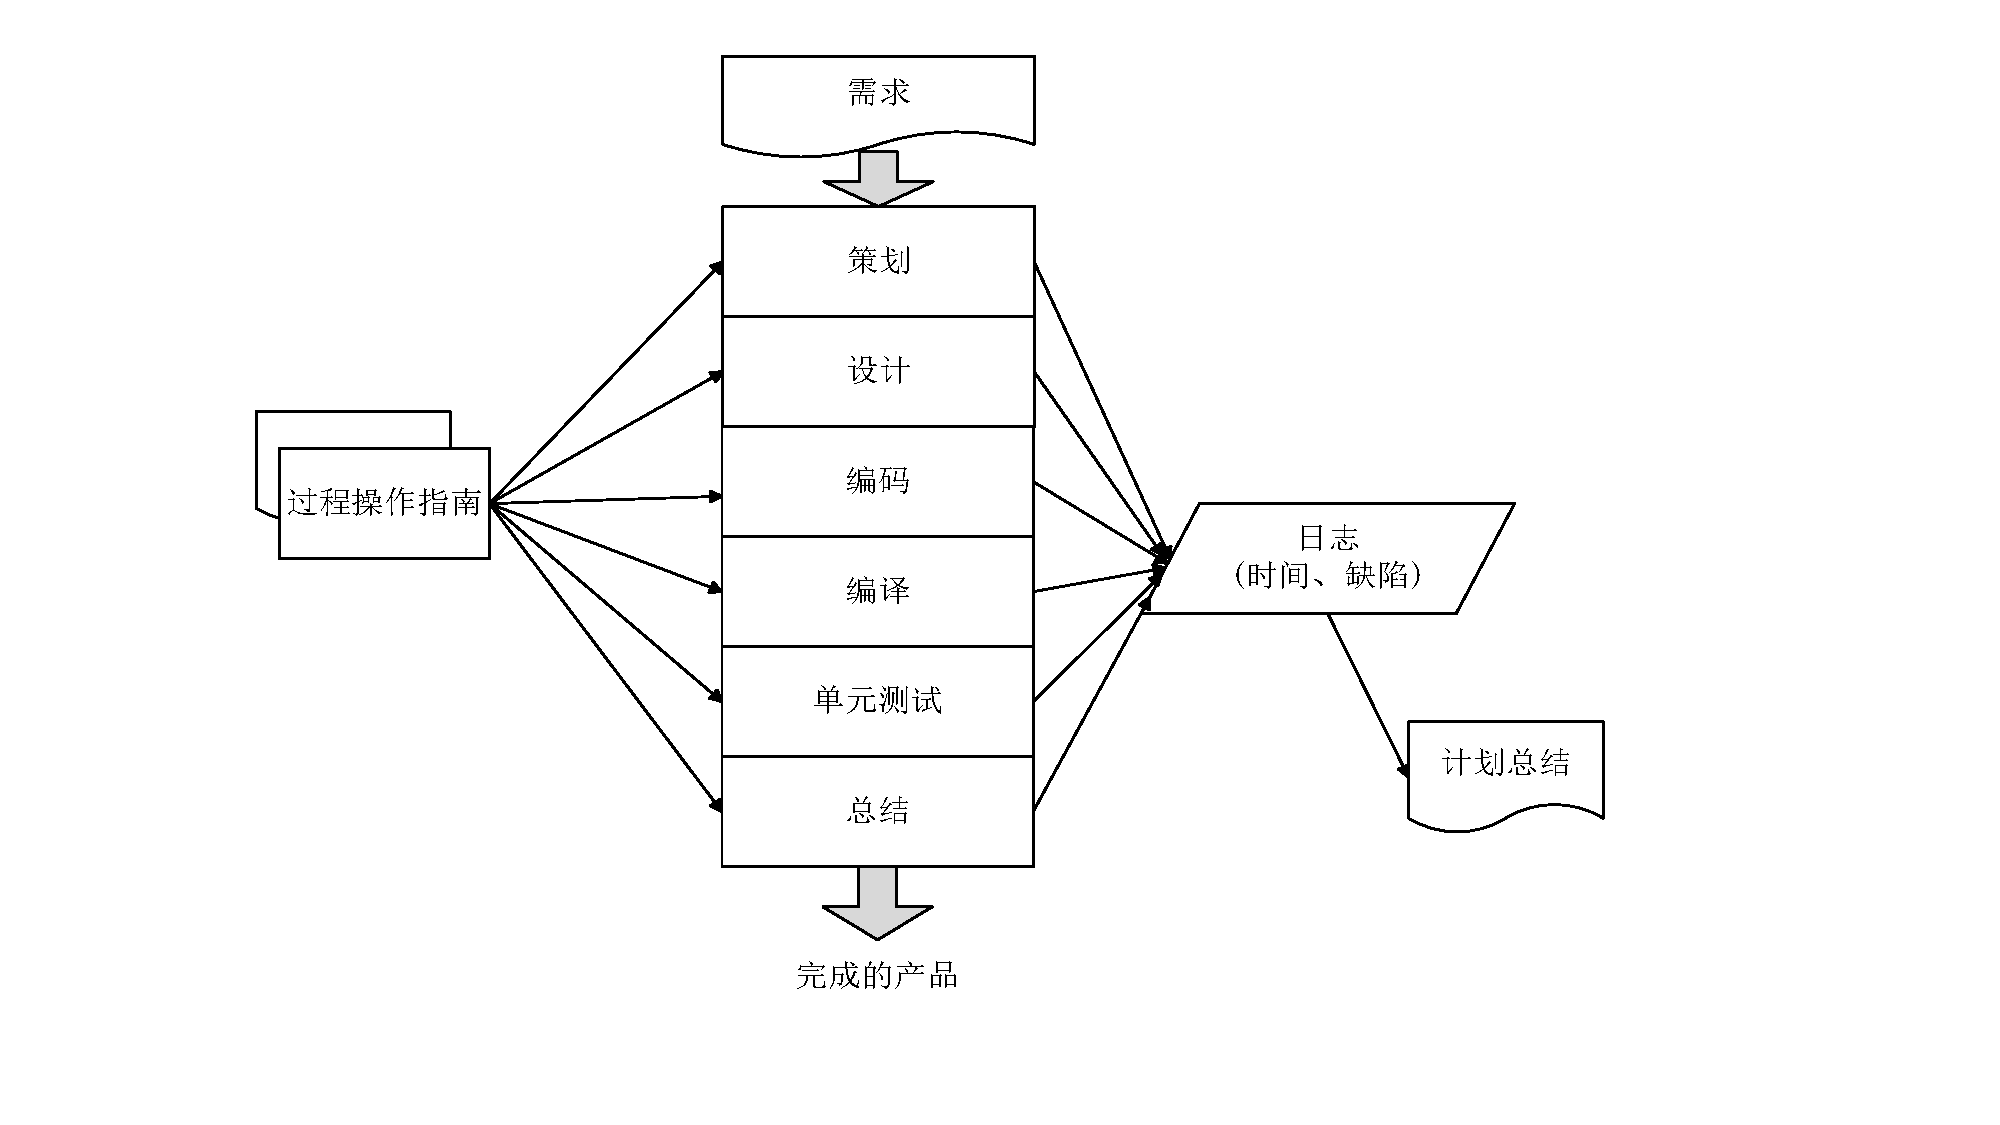
\includegraphics[width=0.7\textwidth]{images/PSP过程.pdf}
    \vspace{-1em}
\end{figure}

\subsubsection{PSP基本原理}
\begin{itemize}
    \item 软件系统的整体质量由该系统中质量最差的某些组件所决定
    \item 软件组件的质量取决于开发工程师所使用的开发过程
    \item 软件工程师应当自己度量、跟踪自己的工作流程,并建立持续的自我改进机制(在自己开发过程的偏差中学习、总结,并将这些经验教训整合到自己的开发实践),自己管理软件组件的质量
\end{itemize}
上述基本原理除了继续肯定“过程质量决定最终产品质量”这一软件过程改进的之外,更加突出了个体软件工程师在管理和改进自身过程中的能动性。这就形成了PSP的理论基础

\subsubsection{PSP的成熟度级别}
\begin{figure}[H]
    \vspace{-0.5em}
	\centering
	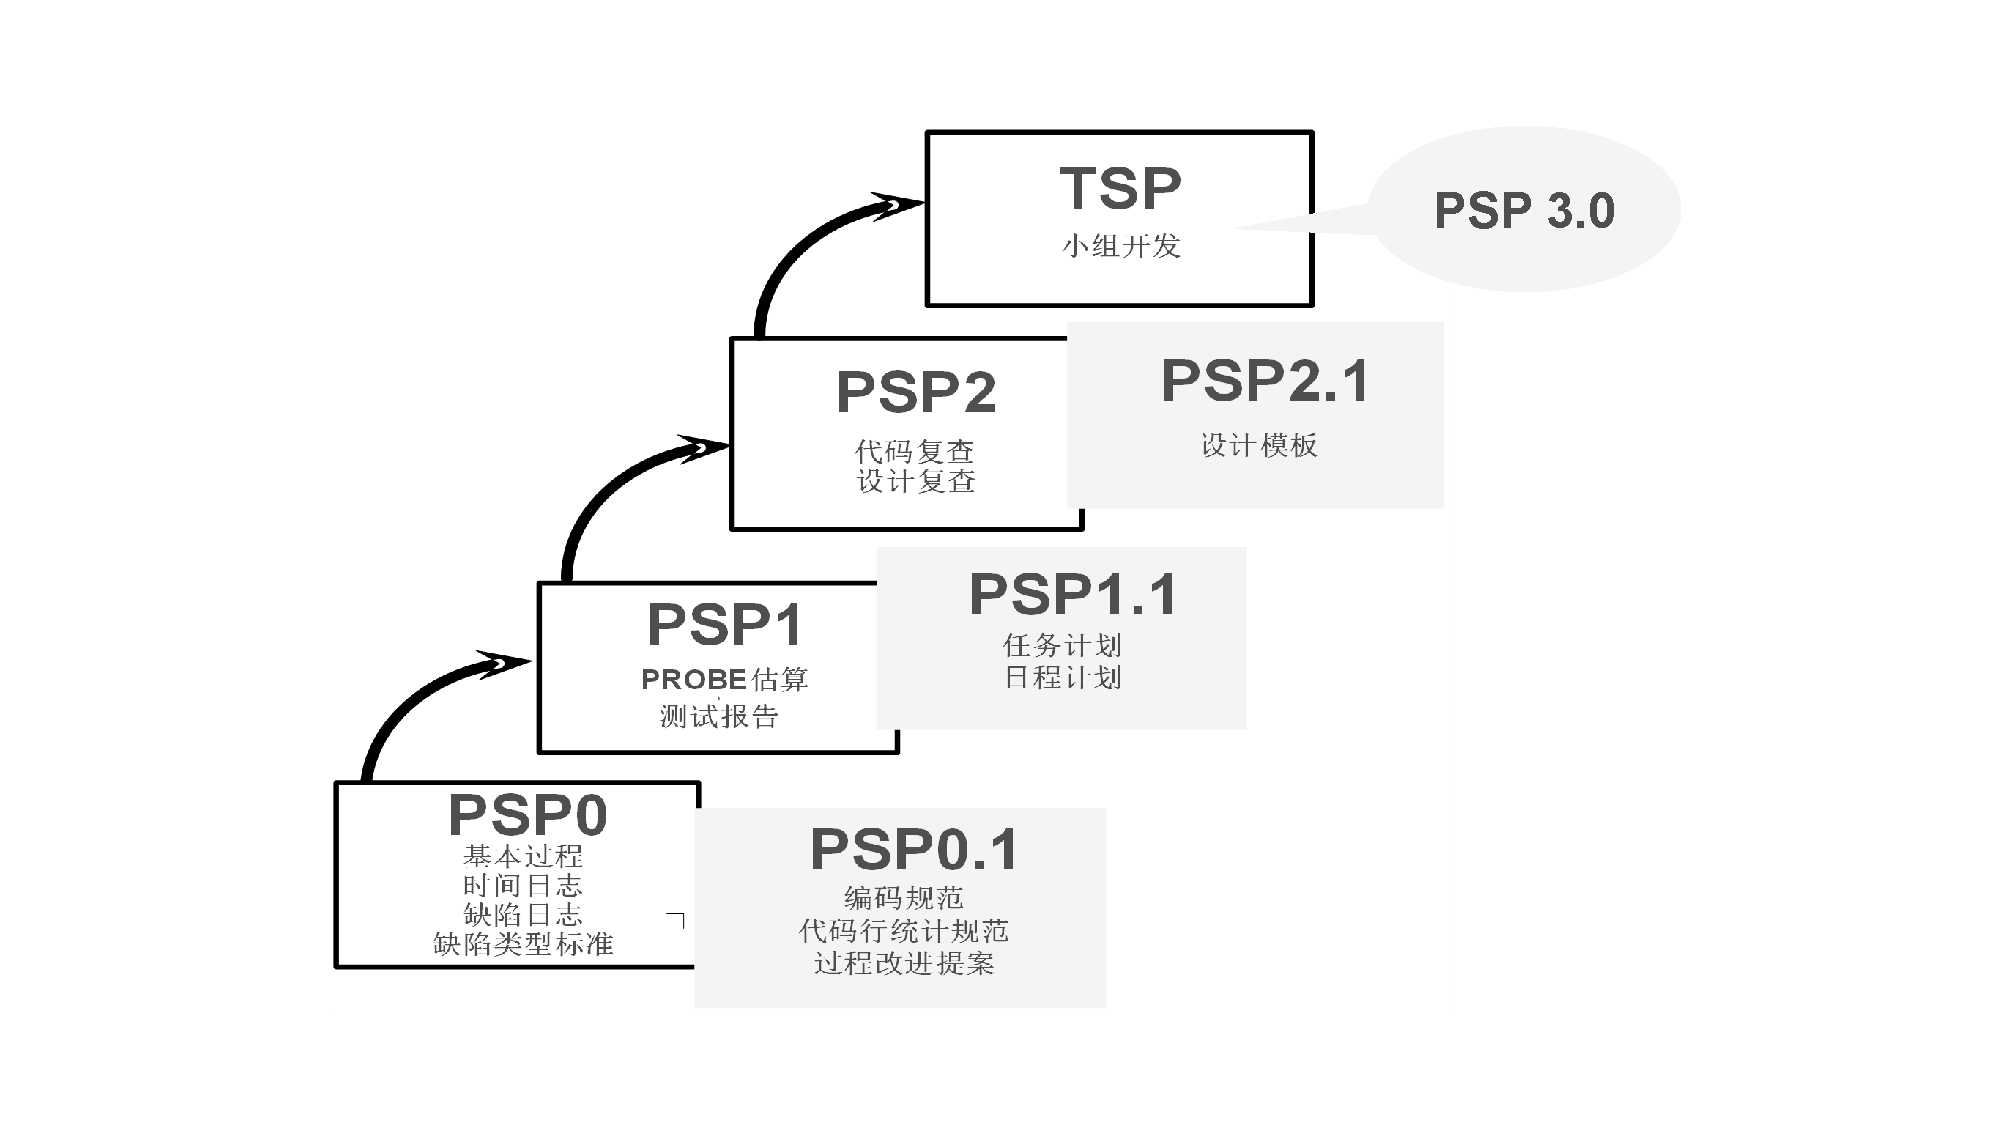
\includegraphics[width=0.6\textwidth]{images/PSP的不同级别.pdf}
    \vspace{-1em}
\end{figure}

\subsection{PSP的度量}

\subsubsection{基本度量项}
\begin{itemize}
    \item 度量时间:序号、所属阶段、开始时间、结束时间、中断时间、净时间、中断原因
    \item 度量缺陷:序号、发现日期、注入阶段、消除阶段、消除时间、关联缺陷、缺陷产生原因
    \item 度量规模:使用PROBE方法
    \vspace{-0.8em}
    \begin{multicols}{2}
        \begin{itemize}
            \item 选择的规模度量方式必须反映开发成本
            \item 度量规模必须被精确定义
            \item 度量规模必须有自动化方法统计
            \item 有助于早期规划
        \end{itemize}
    \end{multicols}
    \vspace{-1em}
    \item 日程(TSP)
\end{itemize}

\subsubsection{度量的作用}
\begin{itemize}
    \item 度量体现着决策者对试图要实现的目标的关切程度
    \item 度量帮助过程的实践者了解过程状态,理解过程偏差
\end{itemize}

\subsubsection{规模度量标准}
\vspace{-0.8em}
\begin{multicols}{2}
    \begin{enumerate}[label=\arabic*.]
        \item 选择的度量方式必须反映开发成本
        \item 选择的度量方式必须精确
        \item 选择的度量方式必须能用自动化方法来统计
        \item 选择的度量方式必须有助于早期规划
    \end{enumerate}
\end{multicols}
\vspace{-1em}

\subsubsection{规模的度量的困境}
精确的度量方式往往不便于早期规划;有助于早期规划的度量往往难以生成精确度量结果

\subsubsection{考试题目}
\begin{problem}
为什么精确的度量方式往往不便于早期规划,而有助于早期规划的度量往往难以产生精确度量结果?
\end{problem}

\begin{problem}
对比度量方式 LOC 和 FP
\vspace{-0.5em}
\begin{spacing}{1.2}
    \centering
    \begin{longtable}{|m{2.5cm}<{\centering}|m{5.5cm}|m{4.5cm}<{\centering}|m{1.7cm}|}
        \hline
        \multicolumn{2}{|c|}{LOC}                                                & \multicolumn{2}{c|}{FP}                               \\ \hline
        \multicolumn{1}{|c|}{LOC优点}                 & \multicolumn{1}{c|}{LOC缺点} & \multicolumn{1}{c|}{FP优点} & \multicolumn{1}{c|}{FP缺点} \\ \hline
        LOC是软件开发项目的生成品,容易进行计算
        & 
        \vspace{-1em}
        \begin{enumerate}[label=\arabic*.,leftmargin=1em]
            \item LOC测量依赖于程序设计语言,不同语言产生结果存在偏差
            \item 对代码量少但设计精巧的程序产生不利评判
            \item 不适合非过程语言
            \item 在软件项目开发前或开发初期估算代码行数非常困难
            \vspace{-1.3em}
        \end{enumerate}                           
        & 
        \vspace{-1em}
        \begin{enumerate}[label=\arabic*.,leftmargin=1em]
            \item 和程序设计语言无关
            \item 面向过程和非过程语言均适合
            \item 基于项目开发初期就可能得到的数据
            \vspace{-1.3em}
        \end{enumerate}    
        & 计算基于主观而非客观数据 \\ \hline
    \end{longtable}
	\end{spacing}
\vspace{-1em}
\end{problem}

\begin{problem}
解释过程度量项定义时应当注意的方面,并且据此评价PSP基本度量元的合理之处?
\end{problem}

\begin{problem}
如何对某个软件产品组件进行产品质量评价?可以选择哪些度量元,这些度量元如何辅助判断产品组件的质量?
\end{problem}

\subsection{PROBE方法}
估算的目的是给各类计划提供决策依据

\subsubsection{估算原理}
设置合理的代理作为\textbf{精确度量}和\textbf{早期规划}需要的度量之间的桥梁:相对大小矩阵。相对大小而非绝对大小

\subsubsection{PROBE方法引入}
估算房子面积大小
\vspace{-0.8em}
\begin{multicols}{2}
    \begin{itemize}
        \item 使用房间相对大小矩阵
        \item 使用房间作为代理
    \end{itemize}
\end{multicols}
\vspace{-1em}

\begin{figure}[H]
    \vspace{-0.5em}
	\centering
	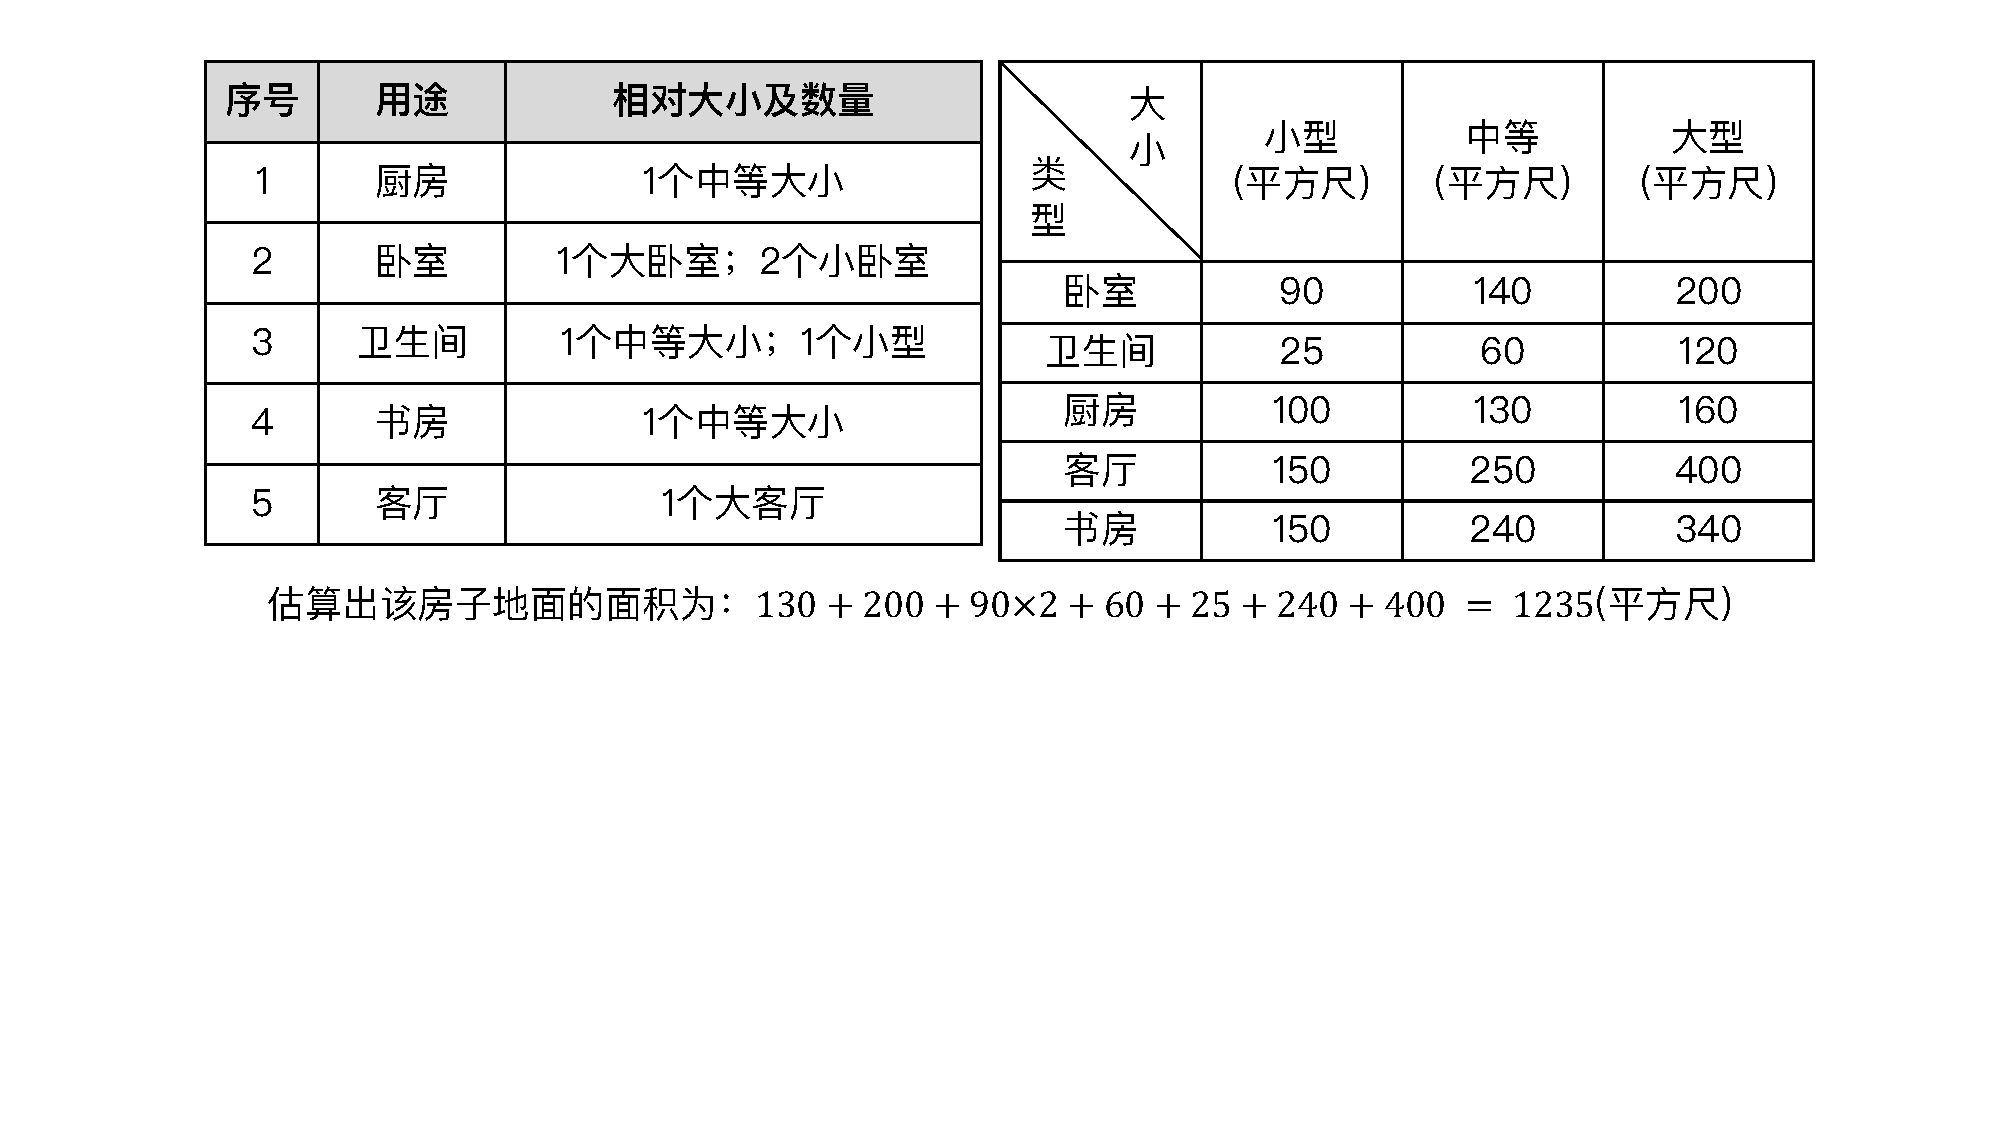
\includegraphics[width=0.95\textwidth]{images/PROBE方法例子.pdf}
    \vspace{-1em}
\end{figure}

\subsubsection{PROBE方法思想}
在PROBE估算中,需要建立自己的代码库,以跟踪所有程序的规模和工作量,而代码库中的每个组件都有设定的类型(计算、逻辑或数据等)和规模(非常小、小、中、大、非常大)
\begin{itemize}
    \item 如果新建立的组件与以前建立的组件类似,那么新组件所需的工作量与旧组件一样
    \item 当开始一个新项目时,我们可以将任务划分成与代码库中组件相似的类型和规模,然后利用线性回归方法来估算项目的工作量
\end{itemize}

估算本质上是一种猜测,追求的目标是一致性以及估算结果的使用者对估算结果的信心
\begin{itemize}
    \item PROBE方法通过定义估算过程和数据收集以及使用的框架,使得估算结果可以尽可能一致,从而使得一些统计方法可以用来调整估算结果,增强用户对估算结果的信心
    \item PROBE方法非常依赖高质量的历史数据,一旦数据不完整或缺失,会导致估算结果有明显偏差
\end{itemize}

\subsubsection{通用计划框架}
\begin{figure}[H]
    \vspace{-0.5em}
	\centering
	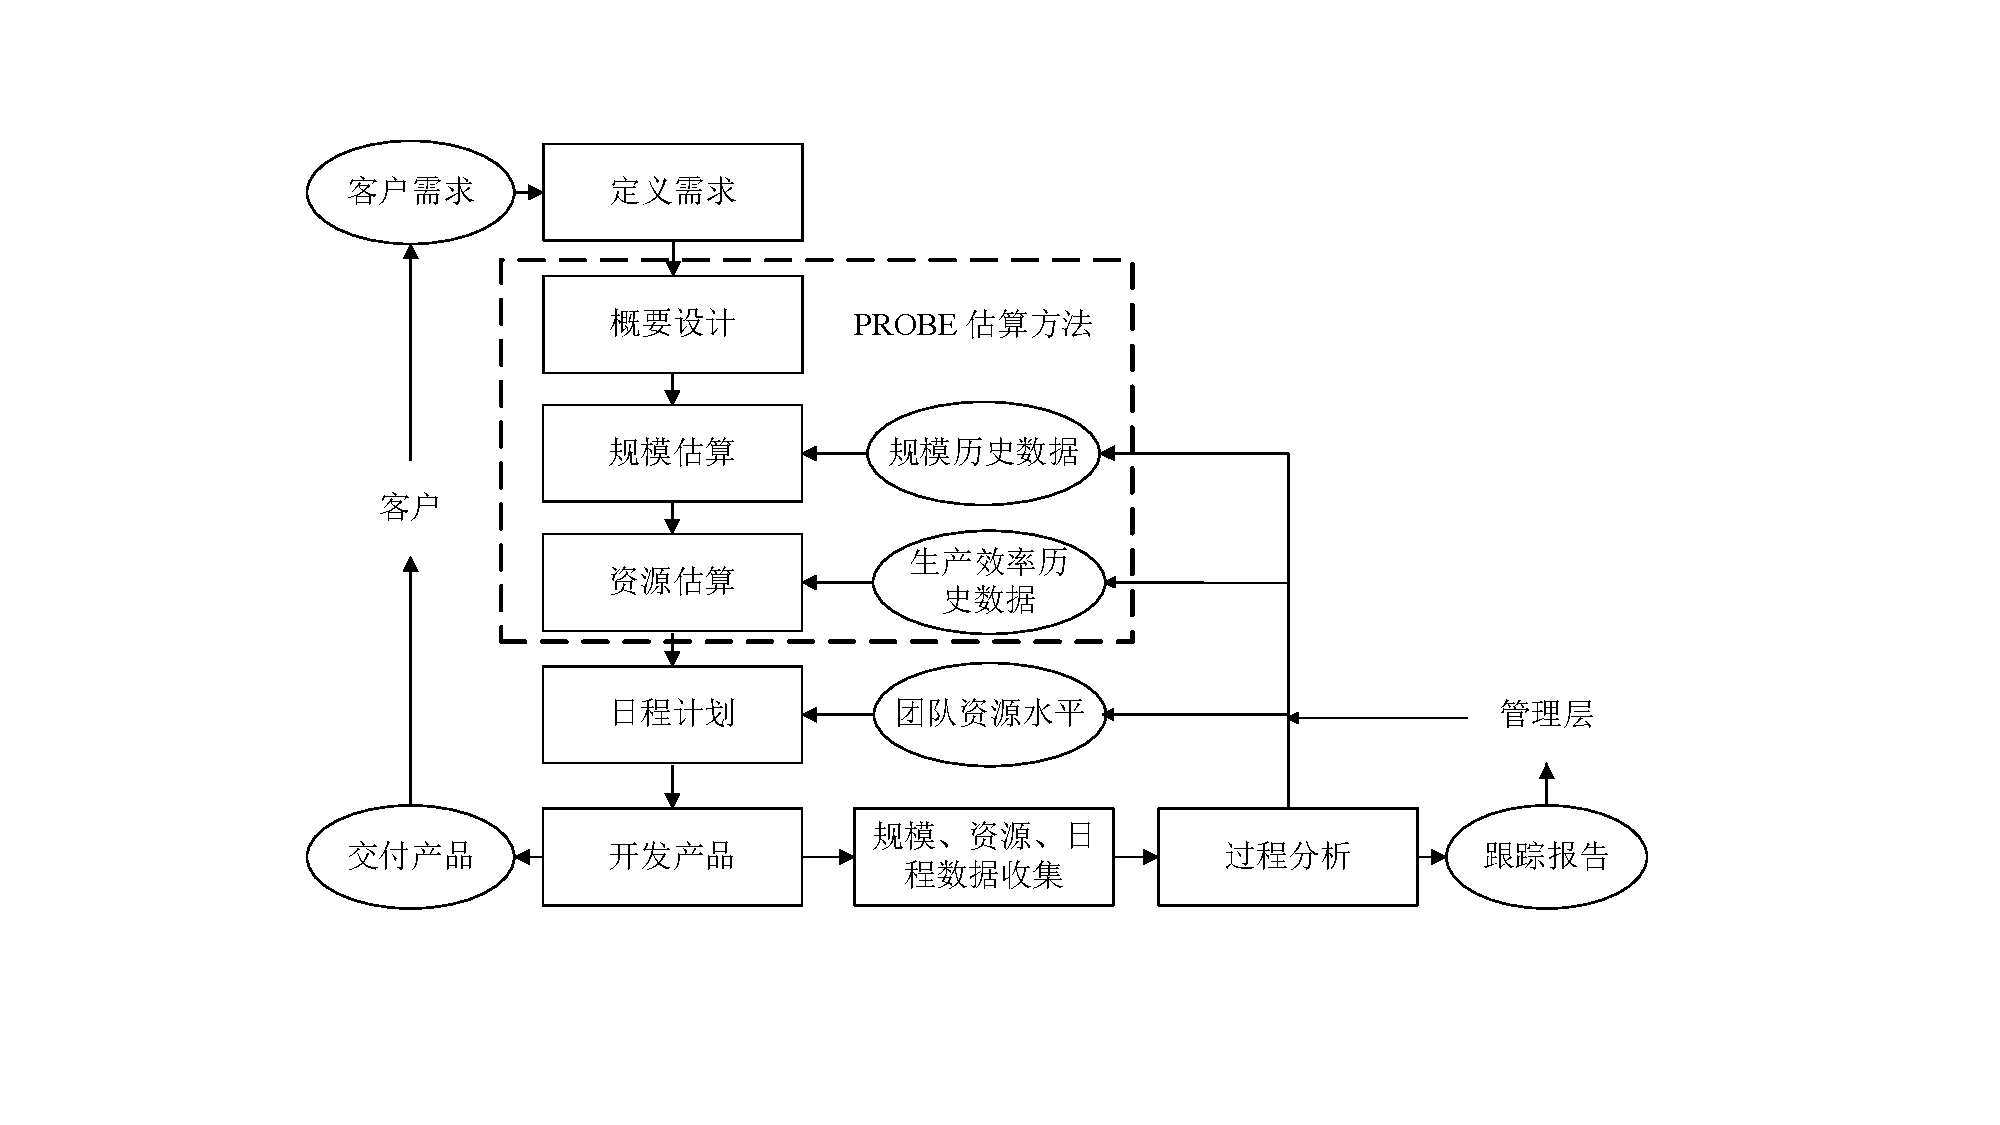
\includegraphics[width=0.75\textwidth]{images/通用计划框架.pdf}
    \vspace{-1em}
\end{figure}

上述框架中,哪些步骤必须人为的干预
\vspace{-0.8em}
\begin{multicols}{2}
    \begin{itemize}
        \item 定义需求
        \item 概要设计:划分由人为开始,规模划分好之后估算是自动产生的
        \item 日程计划
    \end{itemize}
\end{multicols}
\vspace{-1em}

这会带来什么的好处?比较容易扛住别人的质疑
\begin{itemize}
    \item 攻击点:资源和时间是否被高估了
    \item 解决:估算没有代码行,PROBE只有功能点是大中小
\end{itemize}

\begin{problem}
请简要描述按照通用计划框架,为了开发合理的项目计划,应该要做哪些估算?PROBE方法充当什么角色。

估算框架如上图,虚线框即为PROBE,用来完成规模和资源的评估
\end{problem}

\subsubsection{PROBE估算过程}
概要设计:
\vspace{-0.8em}
\begin{multicols}{2}
    \begin{enumerate}[label=\arabic*.]
        \item 确定产品功能,以及产生这些功能所需的程序组件/模块
        \item 将程序组件/模板与你之前写的程序相比较,估算它们的规模
        \item 最后将程序组件/模块估算综合给出总规模
    \end{enumerate}
\end{multicols}
\vspace{-1em}

估算要点:
\vspace{-0.8em}
\begin{multicols}{2}
    \begin{itemize}
        \item 尽可能划分详细一些:估算多个部件的时候,总的误差会比各个部件的误差的总和小
        \item 建立对结果的信心
        \item 依赖数据
        \item 估算要的是过程,而非结果,估算的过程是相关干系人达成一致共识的过程
    \end{itemize}
\end{multicols}
\vspace{-1em}

\paragraph{注意点1:整理历史数据}~{} \par
以估算规模为例,可以假定代理规模与实际程序规模之间存在简单关系映射、正态分布、对数正态分布,也可以假定不知道两者之间的关系,按照线性回归方法进行计算
\vspace{-0.5em}
\begin{spacing}{1.2}
    \centering
    \begin{longtable}{|m{1.5cm}<{\centering}|m{7cm}|m{6cm}|}
        \hline
        \textbf{方法} & \multicolumn{1}{c|}{\textbf{方法描述}} & \multicolumn{1}{c|}{\textbf{方法特点}} \\ \hline
        简单方法
        & 最小值作为$VS$,最大值作为$VL$,中值作为$M$,$VS$与$M$均值作为$S$,$VL$与$M$均值作为$L$
        & 优点:计算简单;缺点:不稳定 \\ \hline
        正态分布法
        & 均值作为$M$,计算标准差$\sigma$,则$S=M-\sigma$,$VS=M-2\sigma$,$L=M+\sigma$,$VL=M+2\sigma$
        & 优点:相对稳定,在历史数据基本符合正态分布的情况下,可以给出非常好的相对大小矩阵 \\ \hline
        对数正态分布法
        & \vspace{-1em}
        \begin{enumerate}[label=\arabic*.,leftmargin=1em]
            \item 以$e$为底计算所有数据的自然对数
            \item 取对数之后的值的均值作为$M$,计算相应标准差$\sigma$,$S=M-\sigma$,$VS=M-2\sigma$,$L=M+\sigma$,$VL=M+2\sigma$
            \item 取反对数
        \vspace{-1.3em}
        \end{enumerate}
        & 优点:更加符合人们对于程序的规模的直观感觉,因为大多数人习惯写很多规模很小的程序,少量规模较大的程序 \\ \hline
        线性回归方法
        & \vspace{-1em}
        \begin{enumerate}[label=\arabic*.,leftmargin=1em]
            \item 计算的时候计算了两组线性回归的参数,也就是项目所需的资源并不是直接由程序规模和历史数据中的生产效率相除得到。程序的复杂度和程序规之间并不是简单的正相关关系。
            \item 线性回归方法估算的是一定概率条件下估算值的分布。例如最终实际程序规模有90\%的可能性落在$(a, b)$区间内
            \item Range为在一定概率条件下的变化区间,而$p$为概率
            \item Variance为扰动程度:有时候,历史数据中的一些极端数据会造成相关性的“假象”,故需要先进行数据除噪
            \vspace{-1em}
            $$\begin{array}{l}
            Plan\ Size = \beta_{0\ size} + \beta_{1\ size}(E) \\
            Plan\ Time = \beta_{0\ time} + \beta_{1\ time}(E) \\
            Range = t(p,df)\delta\sqrt{1 + \frac{1}{n} + \frac{(x_k-x_{avg})^2}{\sum\limits_{i=1}\limits^{n}(x_i-x_{avg})^2}} \\
            Variance = \delta^2 = \frac{1}{n-2}\sum\limits_{i=1}\limits^n(y_i - \beta_0 - \beta_1x_i)^2 \\
            \end{array}$$\vspace{-1.8em}
        \vspace{-1.3em}
        \end{enumerate}
        & \vspace{-1em}
        \begin{enumerate}[label=\arabic*.,leftmargin=1em]
            \item Plan Size和估算的类数量不呈现45度,是受到了估算误差和方法外代码的数量共同影响
            \item 该方法没有使用生产效率进行计算,为什么在PROBE中不使用生产效率?这样子使用好不好?因为Plan Size是在一个范围内波动,生产效率也在一个范围内波动,如果将生产效率作为分母,那么可能会导致更大的误差,也就违背了误差的出发点
            \item 估算能力的强弱关注是多稳定,而不是多接近具体的实际情况
            \vspace{-1.3em}
        \end{enumerate} \\ \hline
    \end{longtable}
	\end{spacing}
\vspace{-1em}

\paragraph{注意点2:处理有限的历史数据}~{} \par
规模估算:
\begin{itemize}
    \item 往往可以依据历史数据来完成,使用代理规模与实际程序规模之间的关系。
    \item 其原因在于规模估算结果的偏差产生原因相对客观,偏差可以用以修正新的估算结果。
    \item 估算规模对历史数据的要求如下,其中$r$为相关性(两组数据之间相互关联的程度,PSP中要求$r\geq 0.7$),其中$S$为显著性(两组数据的相关关系出现的偶然性,PSP要求$s\leq 0.05$)
\end{itemize}

\vspace{-0.5em}
\begin{spacing}{1.2}
    \centering
    \begin{longtable}{|m{2.3cm}<{\centering}|m{3cm}|m{4cm}|m{2.3cm}<{\centering}|}
        \hline
        \textbf{PROBE方法} & \multicolumn{1}{c|}{\textbf{数据要求}} & \multicolumn{1}{c|}{\textbf{数据质量要求}}                                                 & \multicolumn{1}{c|}{\textbf{计算方法}} \\ \hline
        A & 3组或者3组以上代理规模(E)与实际程序规模 &
        \vspace{-1em}
        \begin{enumerate}[label=\arabic*.,leftmargin=1.2em,itemsep=-2pt]
            \item $r\geq 0.7$
            \item $s\leq 0.05$
            \item $\beta 0 \leq$ 估算结果的25\%
            \item $0.5\leq \beta 1 \leq 2$    
        \vspace{-1.3em}
        \end{enumerate}
        & 略 \\ \hline
        B & 3组或者3组以上计划程序规模与实际程序规模 &
        \vspace{-1em}
        \begin{enumerate}[label=\arabic*.,leftmargin=1.2em,itemsep=-2pt]
            \item $r\geq 0.7$
            \item $s\leq 0.05$
            \item $\beta 0 \leq$ 估算结果的25\%
            \item $0.5\leq \beta 1 \leq 2$    
        \vspace{-1.3em}
        \end{enumerate}
        & 略 \\ \hline
        C & 有历史数据 & 无 & 按比例调整 \\ \hline
        D & 没有历史数据 & 无 & 猜测 \\ \hline
    \end{longtable}
	\end{spacing}
\vspace{-1em}

时间估算:
\begin{itemize}
    \item 使用代理规模和实际开发时间的关系。
    \item 时间估算的偏差产生原因更加复杂:一方面和规模有关,另一方面和人的主观能动性有关
    \item 历史数据中的时间偏差可参考价值不大
\end{itemize}

\vspace{-0.5em}
\begin{spacing}{1.2}
    \centering
    \begin{longtable}{|m{2.3cm}<{\centering}|m{3cm}|m{5.7cm}|m{2.3cm}<{\centering}|}
        \hline
        \textbf{PROBE方法} & \multicolumn{1}{c|}{\textbf{数据要求}} & \multicolumn{1}{c|}{\textbf{数据质量要求}}                                                 & \multicolumn{1}{c|}{\textbf{计算方法}} \\ \hline
        A & 3组或者3组以上代理规模(E)与实际程序规模 &
        \vspace{-1em}
        \begin{enumerate}[label=\arabic*.,leftmargin=1.2em,itemsep=-2pt]
            \item $r\geq 0.7$
            \item $s\leq 0.05$
            \item $\beta 0$显著小于估算结果
            \item $\beta 1 \leq 0.5\times$(历史生产效率的倒数)
        \vspace{-1.3em}
        \end{enumerate}
        & 略 \\ \hline
        B & 3组或者3组以上计划程序规模与实际程序规模 &
        \vspace{-1em}
        \begin{enumerate}[label=\arabic*.,leftmargin=1.2em,itemsep=-2pt]
            \item $r\geq 0.7$
            \item $s\leq 0.05$
            \item $\beta 0$显著小于估算结果
            \item $\beta 1 \leq 0.5\times$(历史生产效率的倒数)
        \vspace{-1.3em}
        \end{enumerate}
        & 略 \\ \hline
        C & 有历史数据 & 无 & 按比例调整 \\ \hline
        D & 没有历史数据 & 无 & 猜测 \\ \hline
    \end{longtable}
	\end{spacing}
\vspace{-1em}

\paragraph{注意点3:处理极端数据}~{} \par
极端数据可能造成相关性假象

\subsubsection{考试题目}
\begin{problem}
谈谈你对项目估算的认识,并简要解释应用PROBE方法估算的优缺点
\end{problem}

\begin{problem}
PROBE估算的基本流程
\end{problem}

\begin{problem}
请描述一下PROBE方法的基本原理
\end{problem}

\begin{problem}
请描述一下PROBE方法的过程
\end{problem}

\begin{problem}
使用PROBE方法估算时间的时候,为什么不使用历史数据中的生产效率数据?

在估算资源需求(例如,人时)的时候,生产效率一般在分母上,考虑到个体软件工程师生产效率波动,容易导致估算偏差范围变大。
\end{problem}

\begin{problem}
请描述PROBE ABCD方法在估算规模的时候,对历史数据的质量有什么要求? 
\end{problem}

\begin{problem}
请解释规模估算和资源估算中估算偏差含义之间的差异,并据此简要列举对软件开发活动的启发?

基于风险分析平衡敏捷与规范
\begin{itemize}
    \item 敏捷风险 > 计划驱动风险,启用基于风险的计划驱动方法
    \item 计划驱动风险 > 敏捷风险,启用基于风险的敏捷方法
    \item 不能判断,则通过架构把敏捷部分封装起来,在敏捷部分使用基于风险的敏捷方法,在其他地方启用基于风险的计划驱动方法
\end{itemize}

\begin{figure}[H]
    \vspace{-0.5em}
	\centering
	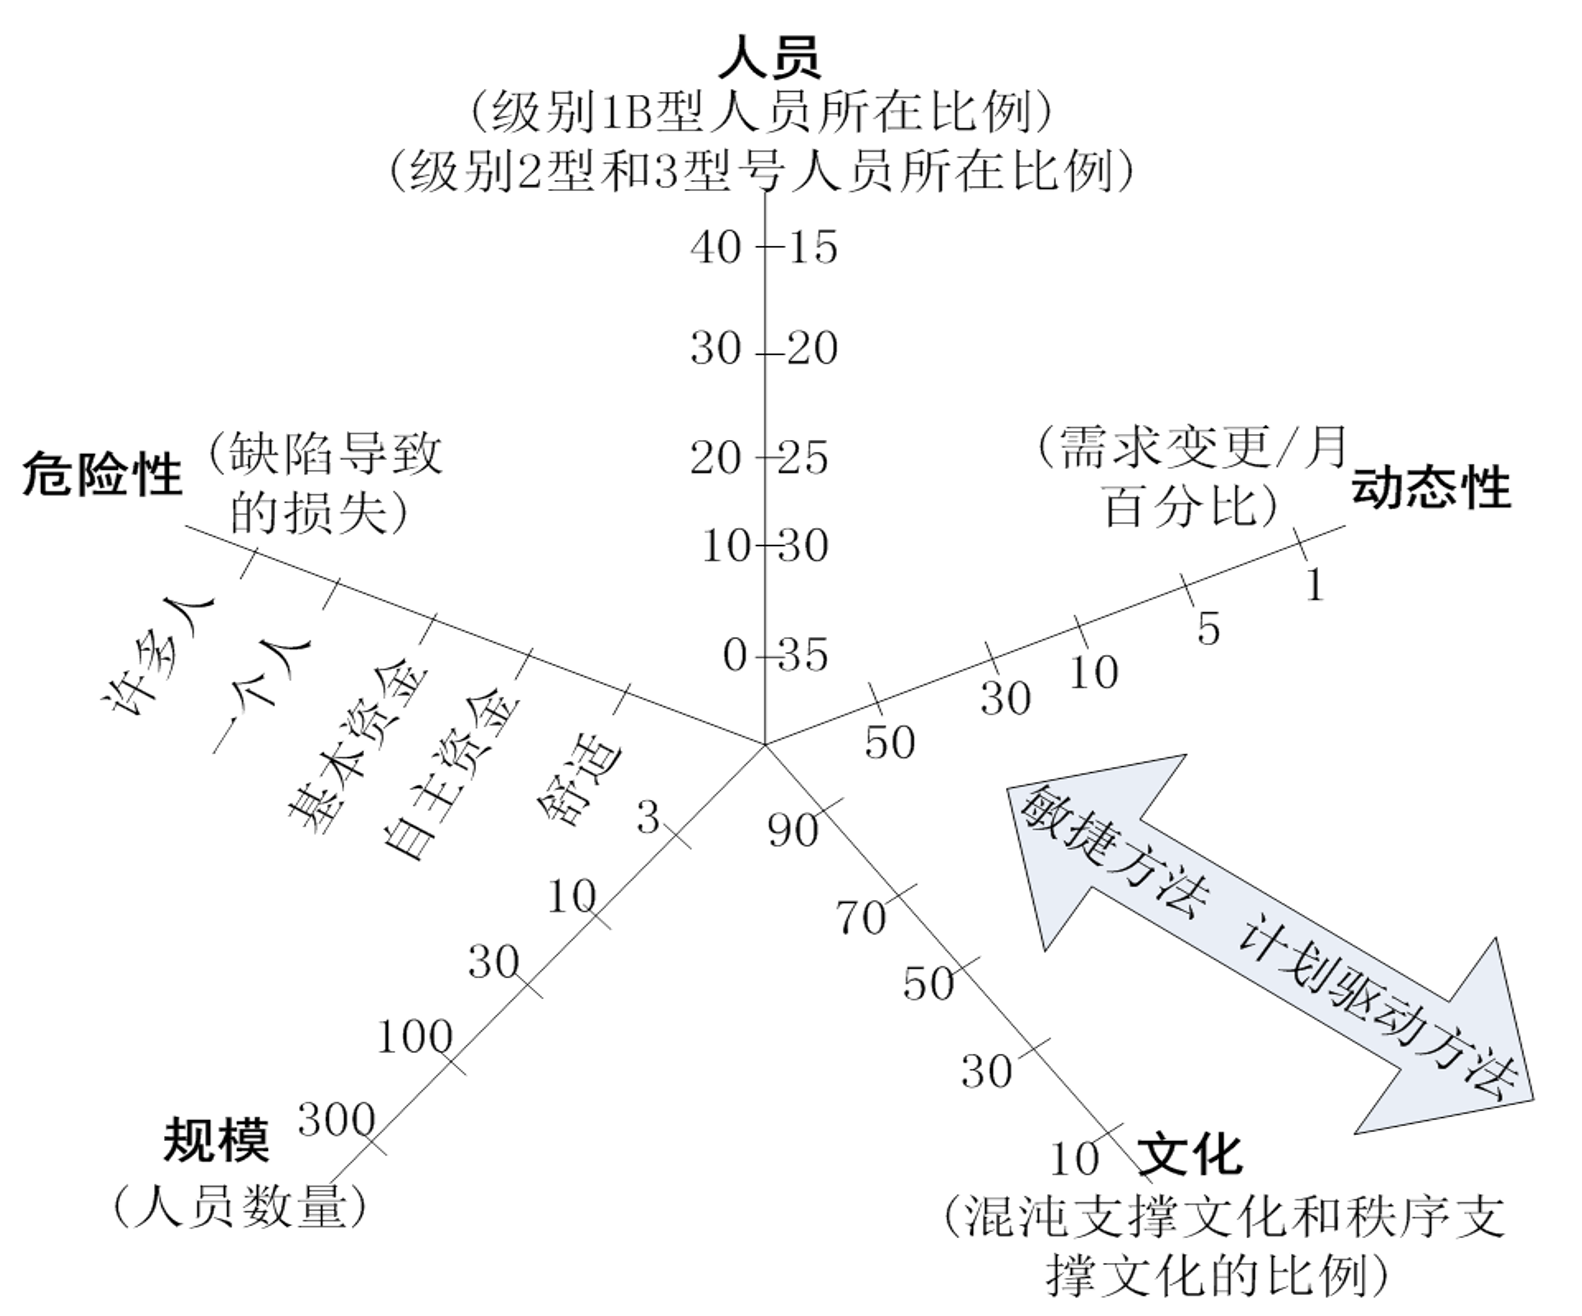
\includegraphics[width=0.55\textwidth]{images/基于风险分析平衡敏捷与规范.png}
    \vspace{-1em}
\end{figure}
\end{problem}

\subsection{PSP的质量管理}

\subsubsection{PSP质量观与质量策略}
软件项目的\textbf{日程、成本以及质量}三大目标统一于质量目标

什么是软件质量?
\begin{itemize}
    \item 与软件产品满足规定的和隐含的需求能力有关的特征或者特征的全体
    \item PSP中定义质量为满足用户需求的程度,需要明确用户需求的\textbf{范围}、\textbf{优先级}、\textbf{度量方式}
\end{itemize}

软件质量分为内外两部分的特性
\vspace{-0.8em}
\begin{multicols}{2}
    \begin{itemize}
        \item 其外部质量特性面向软件产品的最终用户
        \item 其内部质量特性不直接面向最终用户
    \end{itemize}
\end{multicols}
\vspace{-1em}

软件质量的不同视角
\begin{itemize}
    \item 软件质量为软件产品可以改变世界,使世界更加美好的程度。从用户的角度考察软件质量,用户满意度是最为重要的判断标准
    \item 软件质量是对人(用户)的价值,这一定义强调了质量的主观性,即对于同一款软件而言,不同的用户对其质量有不同的体验
\end{itemize}

\paragraph{面向用户的质量观}~{} \par
PSP中也采用了面向用户的质量观,定义质量为满足用户需求的程度。在这个定义中,就需要进一步明确:
\vspace{-0.8em}
\begin{multicols}{2}
    \begin{itemize}
        \item 用户究竟是谁?
        \item 用户需求的优先级是什么?
        \item 这种用户的优先级对软件产品的开发过程产生什么样的影响?
        \item 怎样来度量这种质量观下的质量水平?
    \end{itemize}
\end{multicols}
\vspace{-1em}

典型用户质量期望
\begin{itemize}
    \item 这款软件产品必须能够工作:因此可以使用缺陷管理代替质量管理
    \item 这款软件产品最好有较快的执行速度
    \item 这款软件产品最好在安全性、保密性、可用性、可靠性、兼容性、可维护性、可移植性等表现优异
\end{itemize}

指导意义
\vspace{-0.8em}
\begin{multicols}{2}
    \begin{itemize}
        \item 开发在前,运维在后
        \item \textbf{高质量开发确保DevOps中的价值顺畅流动}
        \item 个体软件工程师技能、过程直接影响产品质量
        \item PSP关注提升个体软件工程师工程技能
    \end{itemize}
\end{multicols}
\vspace{-1em}

\paragraph{质量策略}~{} \par
\vspace{-0.8em}
\begin{multicols}{2}
    \begin{itemize}
        \item 首先确保基本没有缺陷,然后再考察其他的质量目标
        \item 使用缺陷管理来代替质量管理
        \item 高质量的产品也就意味着组成软件产品的各个组件基本无缺陷
        \item 各个组件的高质量是通过高质量评审来实现的
    \end{itemize}
\end{multicols}
\vspace{-1em}

为什么有效?
\begin{itemize}
    \item 提高生产效率,通过关注每个组件的质量,往往可以避免在集成测试和系统测试消除
    \item 大量缺陷,减少消除代价,提升生产效率
\end{itemize}

\paragraph{质量路径 Quality Journey}~{} \par
为了追求极高的质量,你有哪些手段?
\vspace{-0.8em}
\begin{multicols}{2}
    \begin{enumerate}[label=\arabic*.]
        \item 各种测试
        \item 进入测试之前的产物质量提升
        \item 评审过程度量和稳定
        \item 质量意识和主人翁态度
        \item 个体 review 的度量和稳定
        \item 诉诸设计
        \item 缺陷预防
        \item 用户质量关——其他质量属性
    \end{enumerate}
\end{multicols}
\vspace{-1em}

\paragraph{考试题目}~{} \par
\begin{problem}
什么是面向用户的质量观?这对质量管理的策略有什么影响?
\end{problem}

\begin{problem}
请区分质量管理和缺陷管理之间的联系和差异,并解释为何在软件开发中将质量和生产效率两者进行妥协不合适?
\end{problem}

\begin{problem}
为了追求极高的软件产品的质量目标,可能有的方法和这些方法的先后顺序分别是什么?
\end{problem}

\begin{problem}
质量实践和质量管理是不一样的:质量实践包括测试等等,质量管理是对质量的管理,而不是实践,管理必须有上面所说的三个要素
\end{problem}

\subsubsection{发现缺陷的几个示例流程}

\paragraph{测试消除缺陷的典型流程}~{} \par
\vspace{-0.8em}
\begin{multicols}{2}
    \begin{enumerate}[label=\arabic*.]
        \item 发现待测程序的一个异常行为
        \item 理解程序的工作方式
        \item 调试程序,找到出错的位置,确定出错的原因:非常耗时,在项目后期可能会消耗数天甚至数周的时间
        \item 确定修改方案,修改缺陷
        \item 回归测试,以确认修改有效
    \end{enumerate}
\end{multicols}
\vspace{-1em}

\paragraph{评审发现缺陷的典型流程}~{} \par
在如下的步骤中,每一步消耗的时间都不会太多。尽管评审的技能因人而异,但是,通过适当培训和积累,有经验的评审者可以发现80\%左右的缺陷
\vspace{-0.8em}
\begin{multicols}{2}
    \begin{itemize}
        \item 遵循评审者的逻辑来理解程序流程
        \item 发现缺陷的同时,也知道了缺陷的位置和原因
        \item 修正缺陷
    \end{itemize}
\end{multicols}
\vspace{-1em}

\subsubsection{评审与测试}

\paragraph{评审检查表}~{} \par

\begin{figure}[H]
	\centering
	\vspace{-0.5em}	
	\subfloat{
	\begin{minipage}[c]{0.44\linewidth}
	\centering
	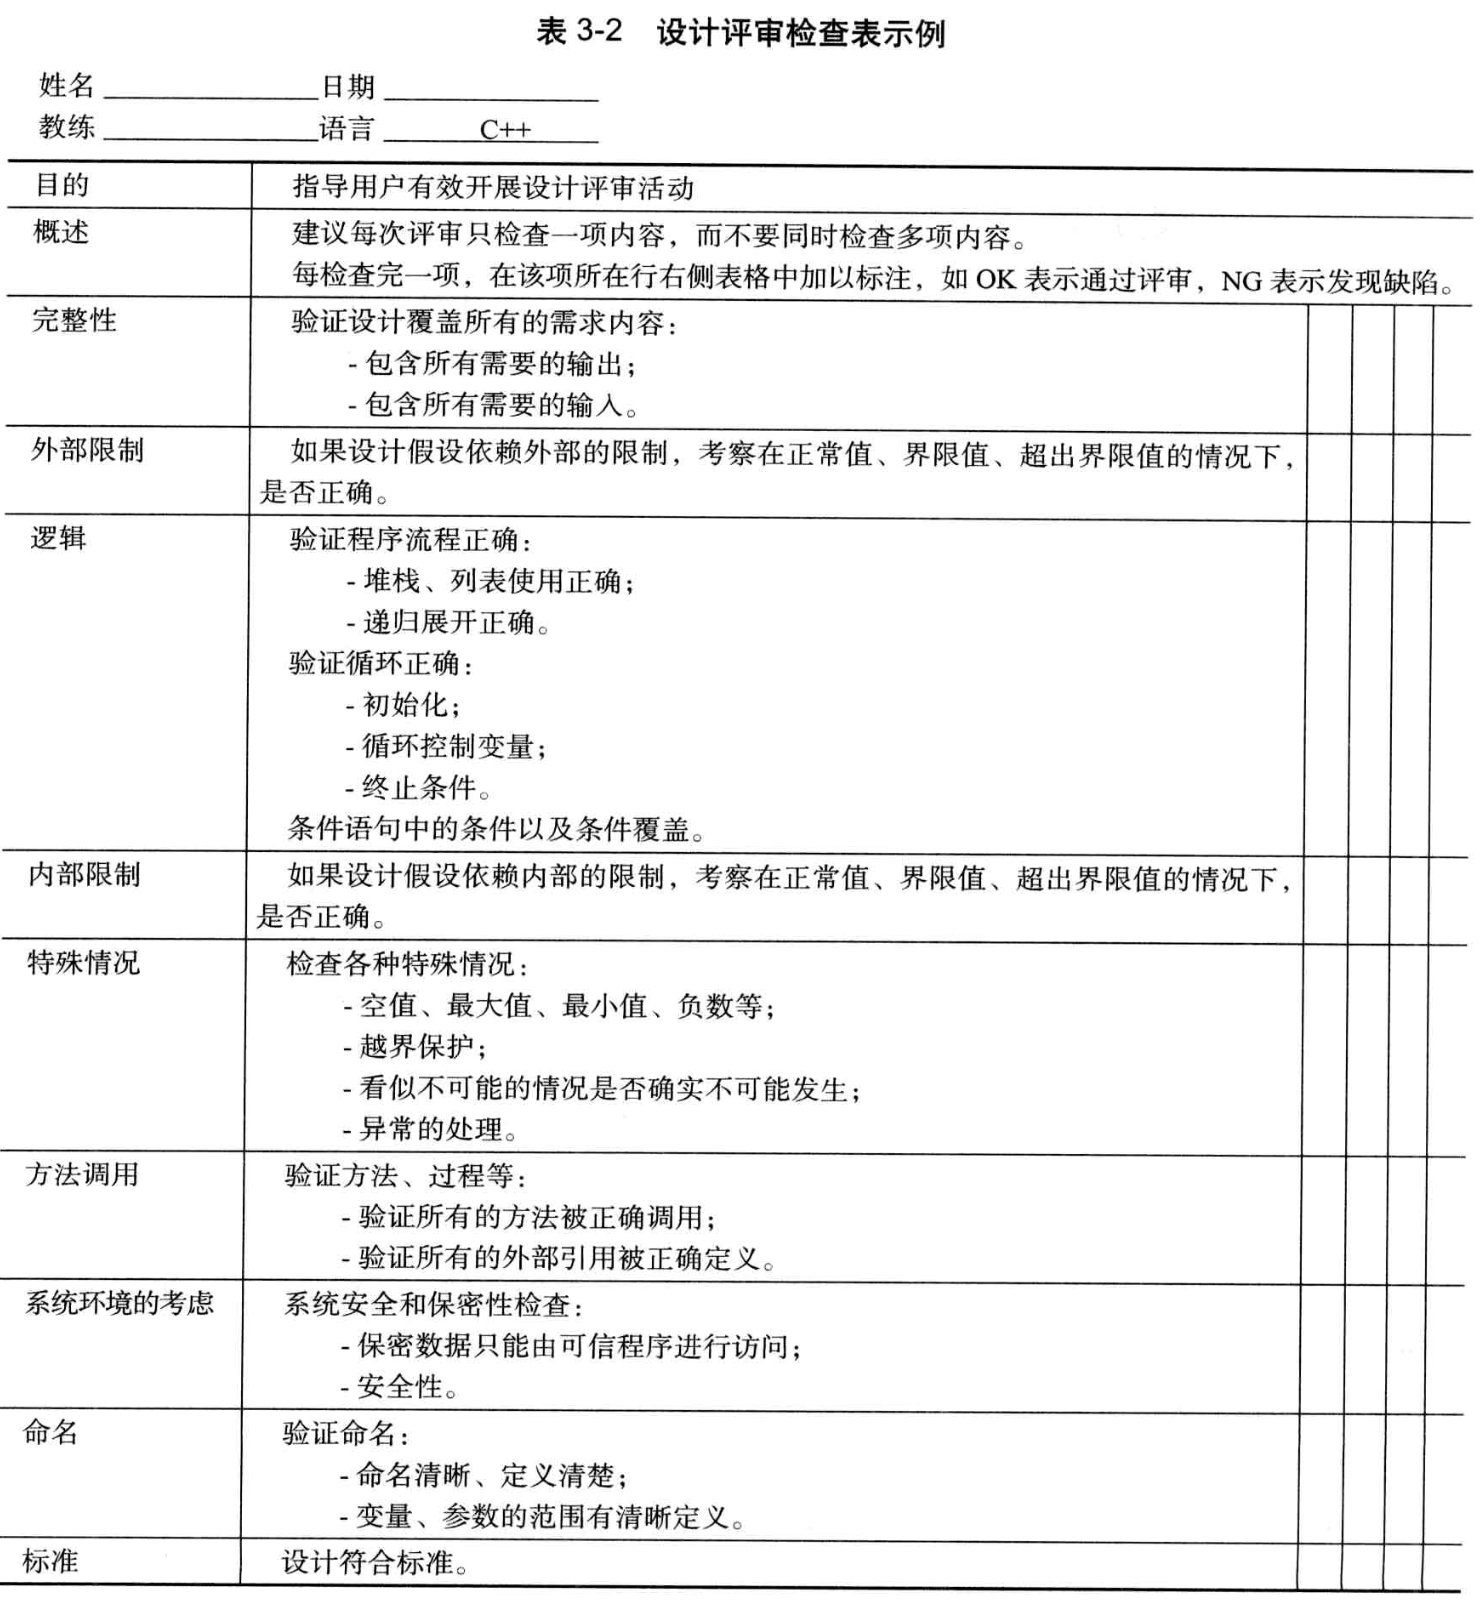
\includegraphics[width=\linewidth]{images/设计评审检查表示例.png}
	\end{minipage}
	}
    \hfill
	\subfloat{
	\begin{minipage}[c]{0.44\linewidth}
	\centering
	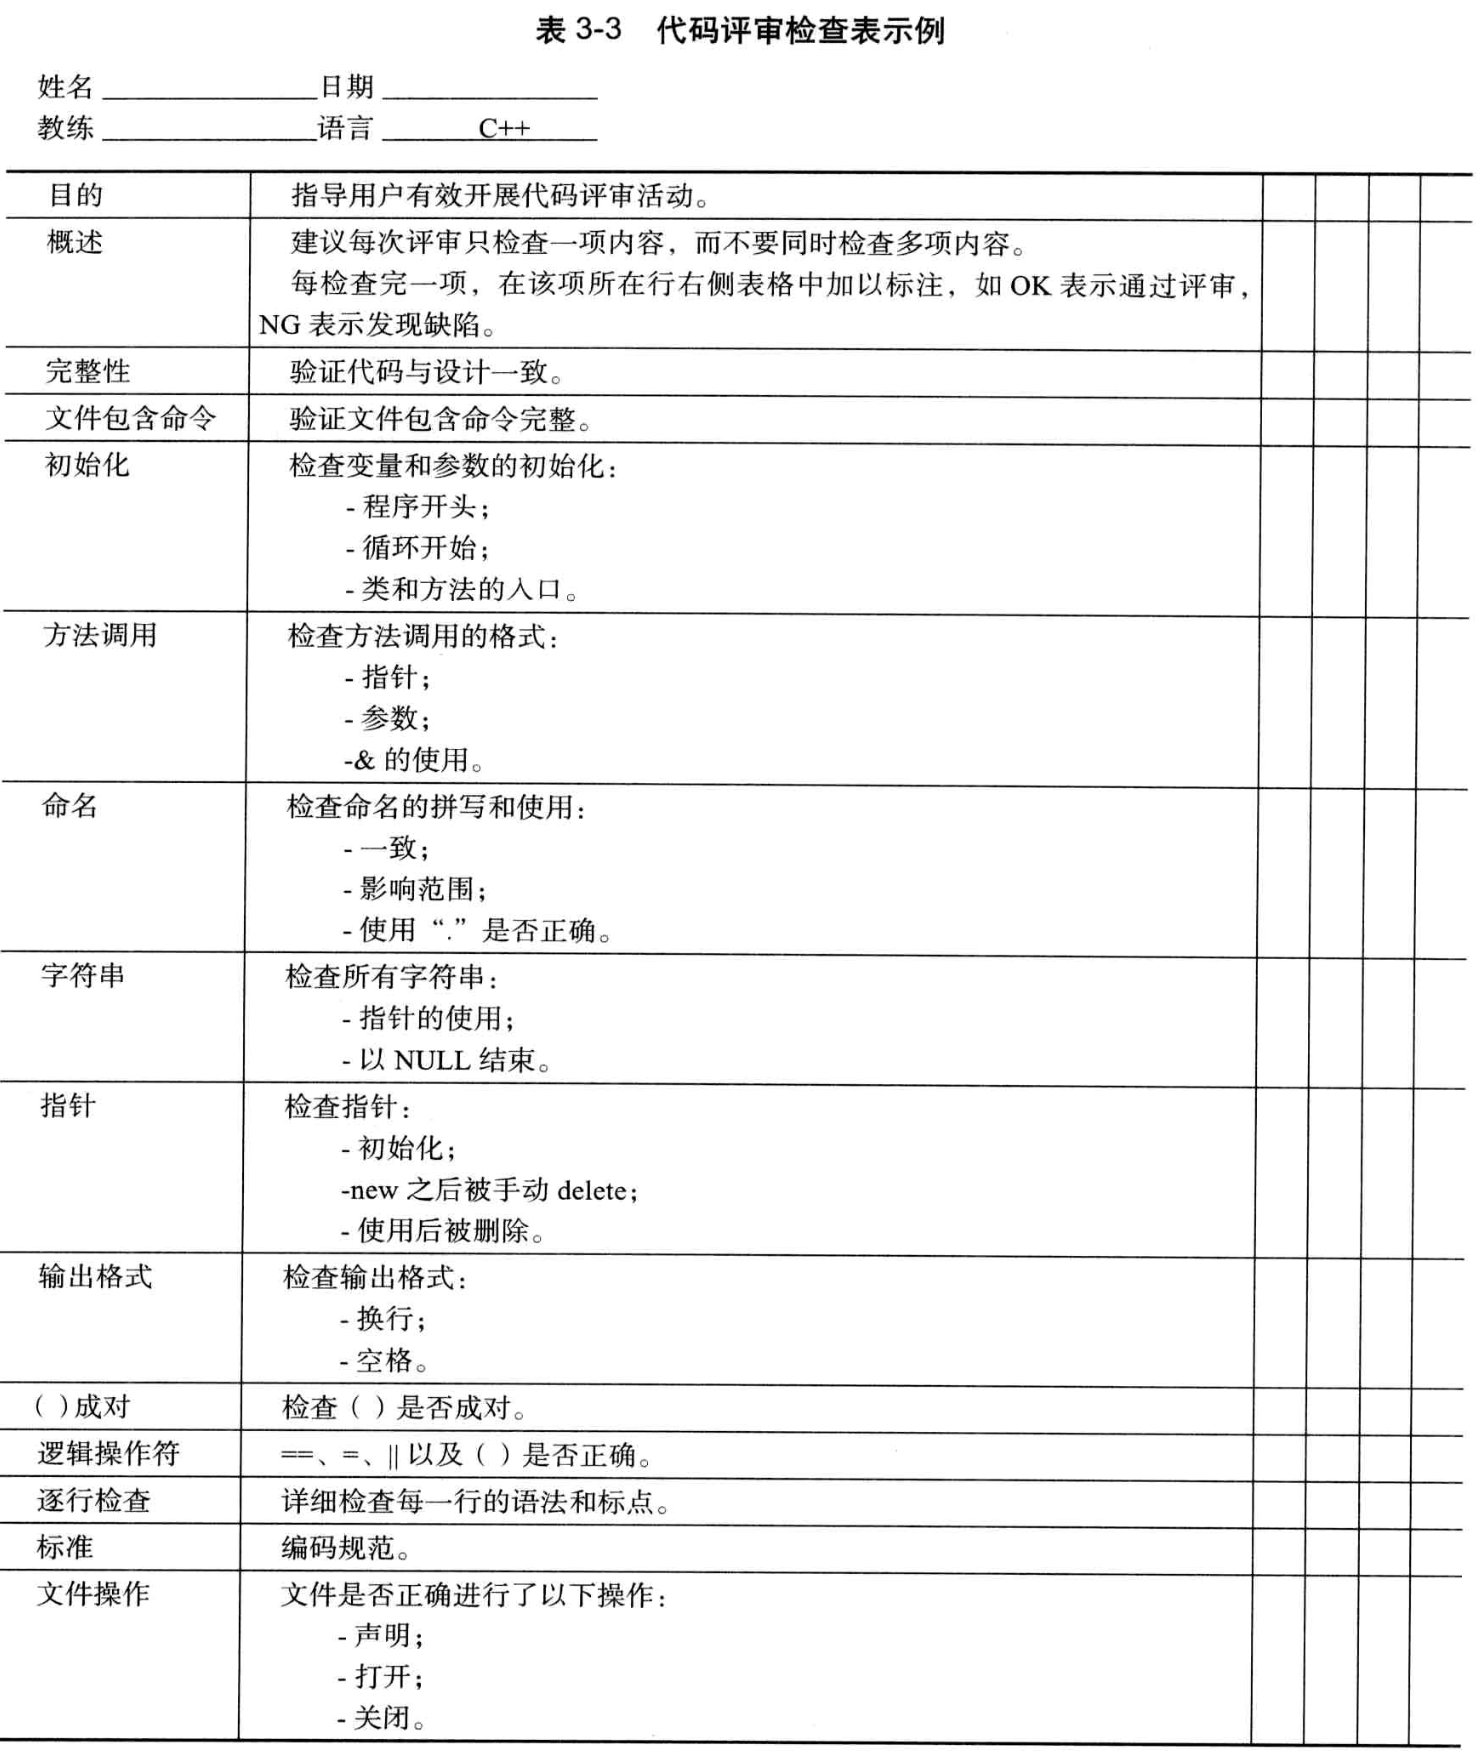
\includegraphics[width=\linewidth]{images/代码评审检查表示例.png}
	\end{minipage}
	}
	\centering
\end{figure}

\paragraph{评审形式}~{} \par
打印后评审效果更好
\begin{itemize}
    \item 单个屏幕可以展现的内容比较有限(评审对象比较复杂的时候,单个屏幕往往不能体现评审对象的整体结构、整体安全、整体性能以及其他整体属性)
    \item 评审人员的注意力:基于屏幕的评审往往容易受到干扰,从而影响评审人员的注意力
\end{itemize}

\paragraph{评审时机}~{} \par
编译、评审
\begin{itemize}
    \item 对于某些类型的缺陷而言,通过编译发现并消除的效率往往是通过评审发现并消除的数倍
    \begin{itemize}
        \item 越来越强大的编译器一般可以发现超过90\%的拼写错误
        \item 不管怎么努力,评审还有会遗漏约$20\sim 50$\%的语法错误
        \item 即便编译器遗漏了一些类似语法的错误,这些错误也不难通过单元测试消除
    \end{itemize}
\end{itemize}

评审、编译
\begin{itemize}
    \item 为了确保评审的效率,不管在评审之前有没有编译,评审的速度是一定的,也就意味着评审所需时间是一定的,那么如果先评审后编译,在编译阶段就可以节省较多的时间
    \item 编译器会大概会遗漏9\%左右的缺陷,从前面讨论可知,为了有较高的质量,这些缺陷仍然期望通过评审加以消除
    \item 有数据表明,编译过程中缺陷较多,往往意味着单元测试中缺陷也较多
    \item 即便单元测试也可以发现一些类似语法的错误,但是,毕竟还有些很难发现,而单元测试之后的一些缺陷消除环节的Pahse Yield往往还低于单元测试
    \item 编译之前评审也是一种自我学习的好机会
    \item 干净的编译,即编译过程没有缺陷对于软件工程师来说,也有极大的成就感
\end{itemize}

\paragraph{评审的具体形式}~{} \par
个人评审 $\rightarrow$ 小组评审

小组评审的意义
\begin{itemize}
    \item 有利于更好地发现缺陷,预防风险,提高Process Yield进而确保质量
    \item 在个人评审之后安排小组评审,也有利于提升个人的技能。特别是那些个人评审未发现而小组评审发现的缺陷,往往都需要引起足够的注意。软件工程师通过对这些缺陷的分析,往往可以学到很多东西
\end{itemize}

\paragraph{评审中缺陷预防过程中的缺陷数据选择}~{} \par
\begin{itemize}
    \item 选择那些在系统测试、验收测试以及应用环节出现的缺陷,特别是验收测试和应用环节中的缺陷,这些缺陷往往意味着软件开发过程本身有不足之处
    \item 选择那些在出现频率较高或者消除代价较高的缺陷,这些缺陷如果可以预防,往往可以节省较多开发的代价,从而体现缺陷预防的优势
    \item 选择那些预防方法容易识别和实现的缺陷,这样的策略容易让软件工程师迅速看到缺陷预防的好处,鉴定使用缺陷预防策略的信心
\end{itemize}

\subsubsection{PSP质量控制的衍生指标}

\paragraph{Yield指标}~{} \par
定义了各个阶段在消除缺陷方面的效率:Yield指标越高越好,Process Yield我们期望在80以上
$$Phase\ Yield = 100 \times \frac{\mbox{某个阶段发现的缺陷个数}}{\mbox{某个阶段注入的缺陷个数} + \mbox{进入该阶段前遗留的缺陷个数}}$$

$$Process\ Yield = 100 \times \frac{\mbox{第一次编译前发现的缺陷个数}}{\mbox{第一次编译前注入的缺陷个数}}$$

Yield可用于制定质量计划并且在项目执行阶段用于进行风险监控、预测、识别以及控制

\textbf{例:}计算Phase Yield。例如对于编码阶段来说,注入缺陷16个,消除缺陷 2 个,进入编码阶段遗留缺陷 4 个,那么该阶段的Phase Yield 就是10
\vspace{-0.5em}
\begin{table}[H]
    \centering
    \begin{tabular}{|c|c|c|c|c|}
    \hline
    \textbf{阶段名称} & \textbf{注入缺陷数} & \textbf{消除缺陷数} & \textbf{遗留缺陷数} & \textbf{Phase Yield}    \\ \hline
    设计            & 10             & 0              & 10             & 0                       \\ \hline
    设计评审          & 0              & 6              & 4              & $60=100 \times 6/ (0 + 10)$    \\ \hline
    编码            & 16             & 2              & 18             & $10=100 \times 2/(16 + 4)$     \\ \hline
    代码评审          & 0              & 9              & 9              & $50 = 100 \times 9 / (0 + 18)$ \\ \hline
    编译            & 0              & 5              & 4              & $55.6=100\times 5/(0+9)$       \\ \hline
    单元测试          & 1              & 5              & 0              & $100=100 \times 5 / (1 + 4)$   \\ \hline
    \end{tabular}
\end{table}
\vspace{-1em}

\textbf{例:}不使用历史数据的计算方法:
\begin{itemize}
    \item 在进行各个阶段Yield值的估算时,可以将单元测试阶段的Phase Yield设定为50
    \item 有资料表明,在测试中每发现一个缺陷,往往意味着还有一个缺陷没有被发现
    \item 那么也就意味着在上面的例子中,总共还有5个缺陷末被消除。将5个缺陷按照比例分配到各个缺陷的注入阶段,就可以重新计算Phase Yield的估算值
\end{itemize}

\vspace{-0.5em}
\begin{table}[H]
    \centering
    \begin{tabular}{|c|c|c|c|c|}
    \hline
    \textbf{阶段名称} & \textbf{注入缺陷数} & \textbf{消除缺陷数} & \textbf{遗留缺陷数} & \textbf{Phase Yield}    \\ \hline
    设计            & 11.85             & 0              & 11.85             & 0                       \\ \hline
    设计评审          & 0              & 6              & 5.85              & 50.6    \\ \hline
    编码            & 19             & 2              & 22.85             & 8     \\ \hline
    代码评审          & 0              & 9              & 13.85              & 41 \\ \hline
    编译            & 0              & 5              & 8.85              & 55.6     \\ \hline
    单元测试          & 1.15             & 5              & 5              & 50   \\ \hline
    \end{tabular}
\end{table}
\vspace{-1em}

Yield的计算是一种事后的质量控制手段,而且除非发现了所有的缺陷,否则很难非常精确地进行计算

\begin{problem}
基于Yield指标构建缺陷预测模型,并列举该模型的可能改进方案

总体思想:利用回归技术预测软件开发过程中各阶段的Inject Rate(缺陷注入率)和Yield(缺陷消除率)

Yield指标只能用来估算,不可以用来度量。结合Yield指标和下图,只需要知道如下指标就可以基于Yield指标构建一个基本的缺陷预测模型:
\vspace{-0.8em}
\begin{multicols}{2}
    \begin{itemize}
        \item 注入阶段注入多少缺陷
        \item 缺陷注入的密度(需求每一页注入多少缺陷)
        \item 缺陷注入的速度(每小时注入多少缺陷)
        \item 消除阶段的缺陷注入密度和速度。
        \item 历史数据中的软件规模、文档规模、开发人员规模
    \end{itemize}
\end{multicols}
\vspace{-1em}

步骤:
\vspace{-0.8em}
\begin{multicols}{2}
    \begin{enumerate}[label=\arabic*.]
        \item 确定纳入影响因子的数据以及数据度量方法
        \item 从系统历史库中收集历史数据,并进行整理
        \item 依照回归技术进行计算
        \item 在项目进行过程中不断收集数据,与预测数据进行比较,调整回归参数
        \item 项目过程中依据实际数据与预测数据的误差进行风险的预防、识别和控制
    \end{enumerate}
\end{multicols}
\vspace{-1em}

下图第一个消除步骤是需求评审,第二个消除步骤是设计评审,第三个消除步骤是测试评审

\begin{figure}[H]
    \vspace{-0.5em}
	\centering
	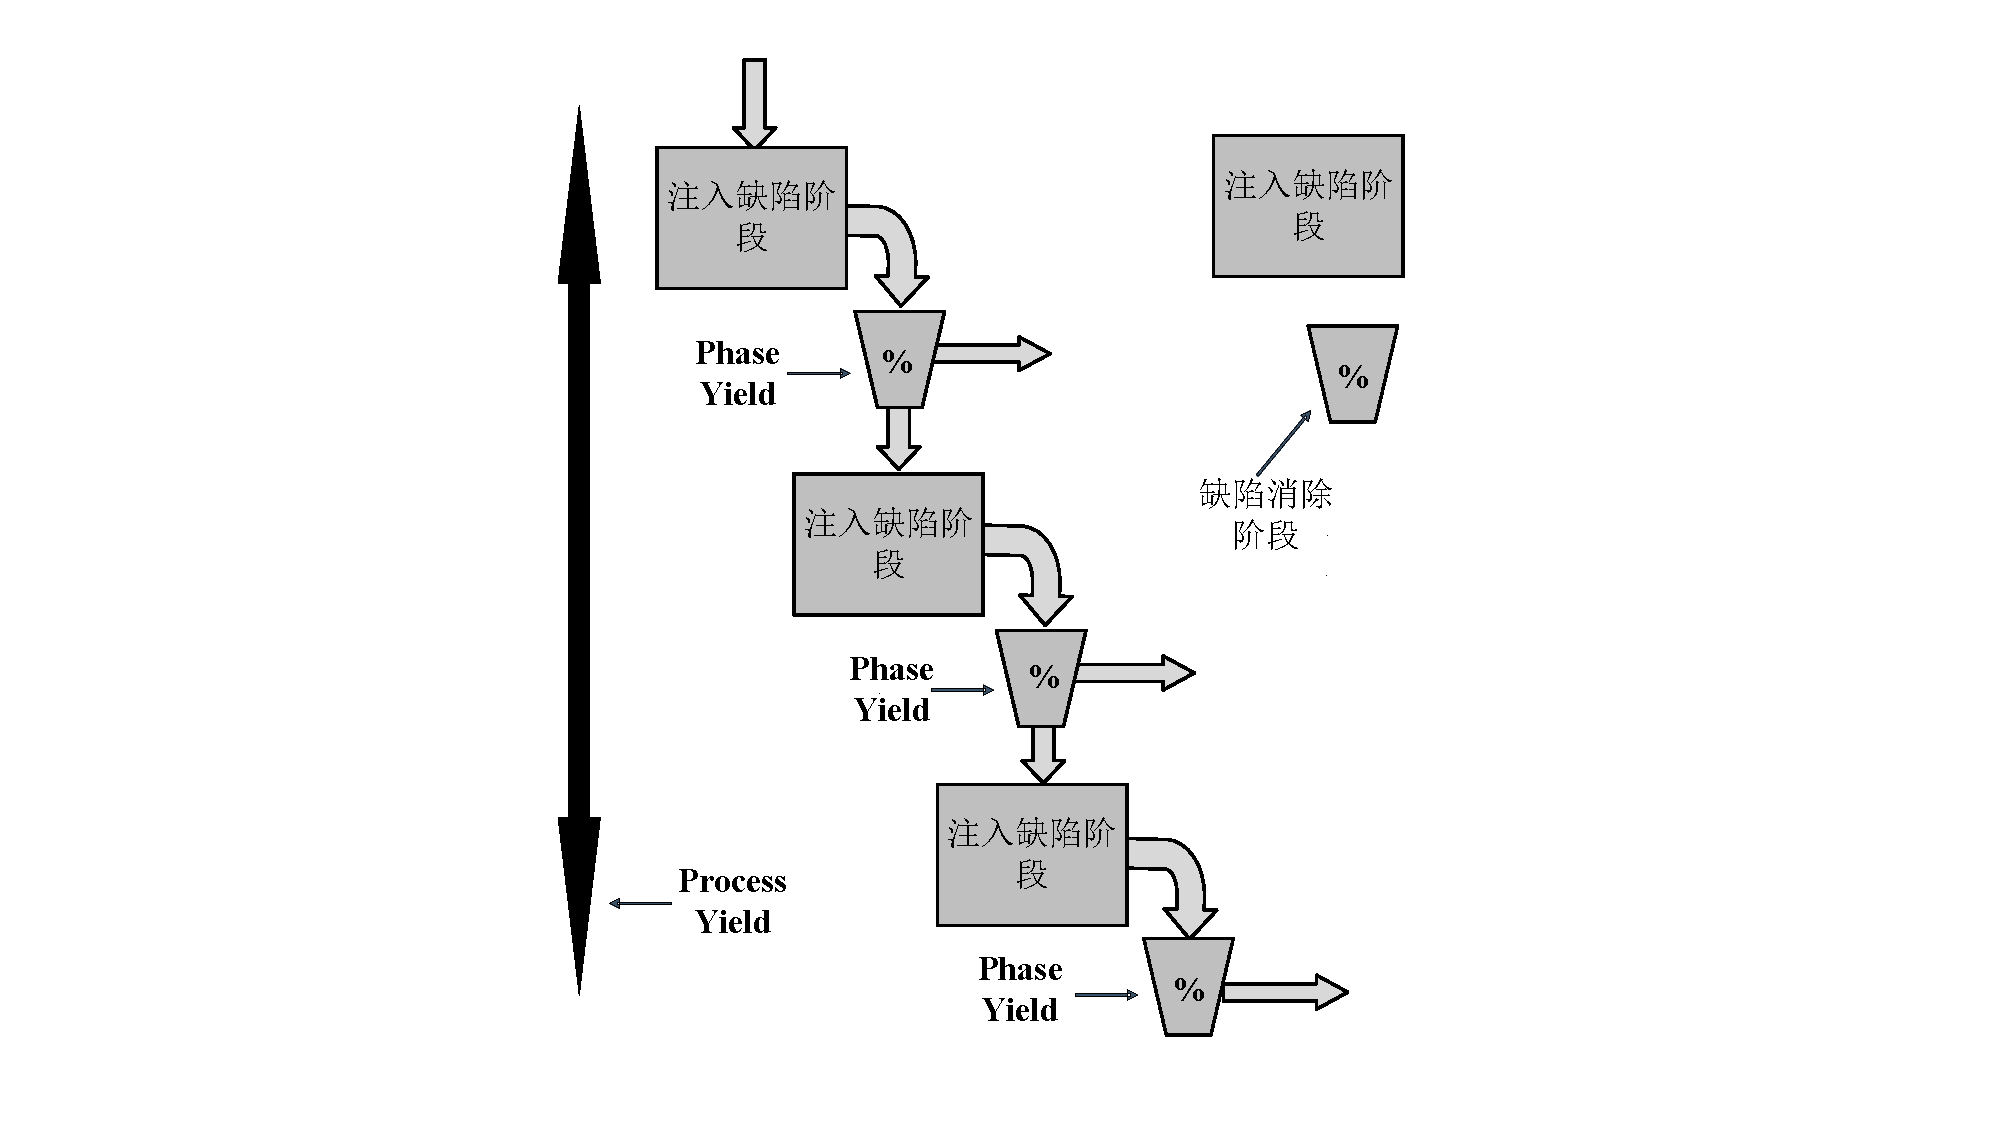
\includegraphics[width=0.42\textwidth]{images/缺陷在开发过程中注入和消除的示意图.pdf}
    \vspace{-1em}
\end{figure}

改进方案:
\begin{itemize}
    \item 结果受限于历史数据在简单性、可理解性、稳定性、可度量性、相关性等方法的质量。因此,维护历史数据。
    \item 影响因子的选择上面不仅仅需要有关软件规模的数据,还需要有关开发过程、开发文档、开发人员等方面的数据,并且需要将数据可度量化。
    \item 反馈模型。即在开发过程中随着实际数据的产生,将这些数据作为输入变量放入模型中以调整回归参数。
    \item (重要)可能的改进是假设注入水平和消除水平都符合正态分布,计算均值和标准差,因此,可以用蒙特卡罗方法模拟结果。
\end{itemize}
\end{problem}

\paragraph{A/FR}~{} \par
质量成本COQ(Cost of Quality)的三个重要组成部分为
\begin{itemize}
    \item 失效成本:分析失效现象、查找原因,做必要的修改所消耗的成本
    \item 质检成本:评价软件产品,确定其质量状况所消耗的成本
    \item 预防成本:识别缺陷根本原因、采取措施预防其再次发生所消耗的成本
\end{itemize}

A/FR (Appraisal toFailureRatio),质检失效比
\vspace{-0.8em}
\begin{multicols}{2}
    \begin{itemize}
        \item A/FR $=$ PSP质检成本 / PSP失效成本
        \item 质检成本 $=$ 设计评审时间 $+$ 代码评审时间
        \item 失效成本 $=$ 编译时间 $+$ 单元测试时间
    \end{itemize}
\end{multicols}
\vspace{-1em}

理论上,A/FR值越大,意味着质量越高,但A/FR值过大说明评审过多,则开发效率低下,因此PSP中A/FR期望值为2.0

\paragraph{PQI}~{} \par
PQI(Process Quality Index, 过程质量指标)为5个数据的乘积(以基准值作为1,最后结果越接近1,质量越高)
\begin{itemize}
    \item 设计质量:设计时间应该大于编码时间,$\min(\frac{\scriptsize{\mbox{设计时间}}}{\scriptsize{\mbox{编码时间}}}, 1)$
    \item 设计评审质量:设计评审的时间应该大于设计时间的50\%,$\min(2 \times \frac{\scriptsize{\mbox{设计评审时间}}}{\scriptsize{\mbox{设计时间}}}, 1)$
    \item 代码评审质量:代码评审时间应该大于编码时间的50\%,$\min(2 \times \frac{\scriptsize{\mbox{代码评审时间}}}{\scriptsize{\mbox{编码时间}}}, 1)$
    \item 代码质量:代码的编译缺陷密度应当小于10个/千行,$\min(\frac{20}{\scriptsize{\mbox{编译缺陷密度}} + 10}, 1)$
    \item 程序质量:代码的单元测试缺陷密度应当小于5个/千行,$\min(\frac{10}{\scriptsize{\mbox{单元测试缺陷密度}} + 5}, 1)$
\end{itemize}

用途:
\vspace{-0.8em}
\begin{multicols}{3}
    \begin{itemize}
        \item 判断模块开发质量
        \item 规划质量活动计划
        \item 过程改进
    \end{itemize}
\end{multicols}
\vspace{-1em}

\begin{problem}
解释PQI指标,如何计算,如何使用
\end{problem}

\paragraph{Review Rate}~{} \par
评审的速度(Review Rate)是一个用以指导软件工程师开展有效评审的指标,高质量的评审需要软件工程师投入足够的时间进行评审
\begin{itemize}
    \item 在PSP的实践中,代码评审速度小于200 LOC/小时,文档评审速度小于4 Page/小时
\end{itemize}

\paragraph{DRL}~{} \par
\begin{wraptable}{r}{7cm}
    \centering
    \vspace{-1.5em}
    \begin{tabular}{|c|c|c|}
        \hline
        \textbf{阶段} & \textbf{缺陷个数/小时} & \textbf{DRL (UT)} \\ \hline
        设计评审        & 3.6              & 1.03              \\ \hline
        编码评审        & 8                & 2.29              \\ \hline
        单元测试        & 3.5              & 1                 \\ \hline
        \end{tabular}
    \vspace{-1.5em}
\end{wraptable}
缺陷消除效率比(DRL, Defect-Removal-Leverage)度量的是不同缺陷消除手段消除缺陷的效率

计算方法:以某个测试阶段(一般为单元测试)每小时发现的缺陷数为基础,其他阶段每小时发现缺陷数与该测试阶段每小时发现的缺陷的比值就是DRL

\paragraph{考试题目}~{} \par
\begin{problem}
请解释A/FR,PQI的计算方式,并且解释这两个指标有什么用途?
\end{problem}

\begin{problem}
请结合A/FR、PQI、Review Rate、DRL、Yield尽可能具体描述一个软件项目应该如何从多方面来确保开发的高质量?

这些指标既是开发过程中质量管理的一些参考指标,同时也体现在计划安排中应该注意的质量元素。具体如下:
\begin{itemize}
    \item 在项目计划过程中应该安排确保高质量开发结果的活动,例如,按照A/FR、PQI等指标的要求,安排对各类产物(文档和代码)的个人评审和小组评审
    \item 这些评审活动应该满足一定的要求,特别体现在时间方面。例如,评审时间应该多于测试时间的两倍以上(A/FR);评审时间应该是相应开放时间的50\%以上(PQI);评审速度要求(Review Rate)等
    \item 充分借鉴质量指标所体现的开发质量状况,尽早制订相应的质量补救措施。例如,PQI所体现的缺陷密度、所有上述指标的参考值等等。一旦超标,往往意味着质量方面有偏差,应当及时补救
    \item 利用Yield等指标,构建质量预测模型,更加积极(Proactive)地判定和控制开发质量
    \item 依据PQI和Yield指标所体现的信息,通过过程改进来提升开发质量
\end{itemize}
\end{problem}

\subsubsection{考试题目}
\begin{problem}
如果对质量的追求是无止境的,在不考虑资源和成本的前提下,有哪些可能有效的策略?
\vspace{-0.8em}
\begin{multicols}{2}
    \begin{enumerate}[label=\arabic*.]
        \item 重视测试,并且将测试过程文档化并且稳定化
        \item 重视小组评审,同样定义评审过程,并且使得评审过程的performance稳定化
        \item 重视个人评审,提升评审者技能
        \item 重视设计
        \item 开展设计验证
        \item 质量策略:参考上面
    \end{enumerate}
\end{multicols}
\vspace{-1em}
\end{problem}

\subsection{PSP的设计}
PSP设计过程的关注点并不是具体的设计方法,而是设计的步骤定义以及设计的表现形式

\subsubsection{设计与质量的关系}
\vspace{-0.8em}
\begin{multicols}{2}
    \begin{itemize}
        \item 低劣的设计是导致在软件开发中返工、不易维护以及用户不满的主要原因
        \item 充分设计可以显著减少最终程序的规模,提升质量
        \item 设计本身也是一种排除错误的过程
    \end{itemize}    
\end{multicols}
\vspace{-1em}

\subsubsection{设计的过程}
\begin{figure}[H]
    \vspace{-0.5em}
	\centering
	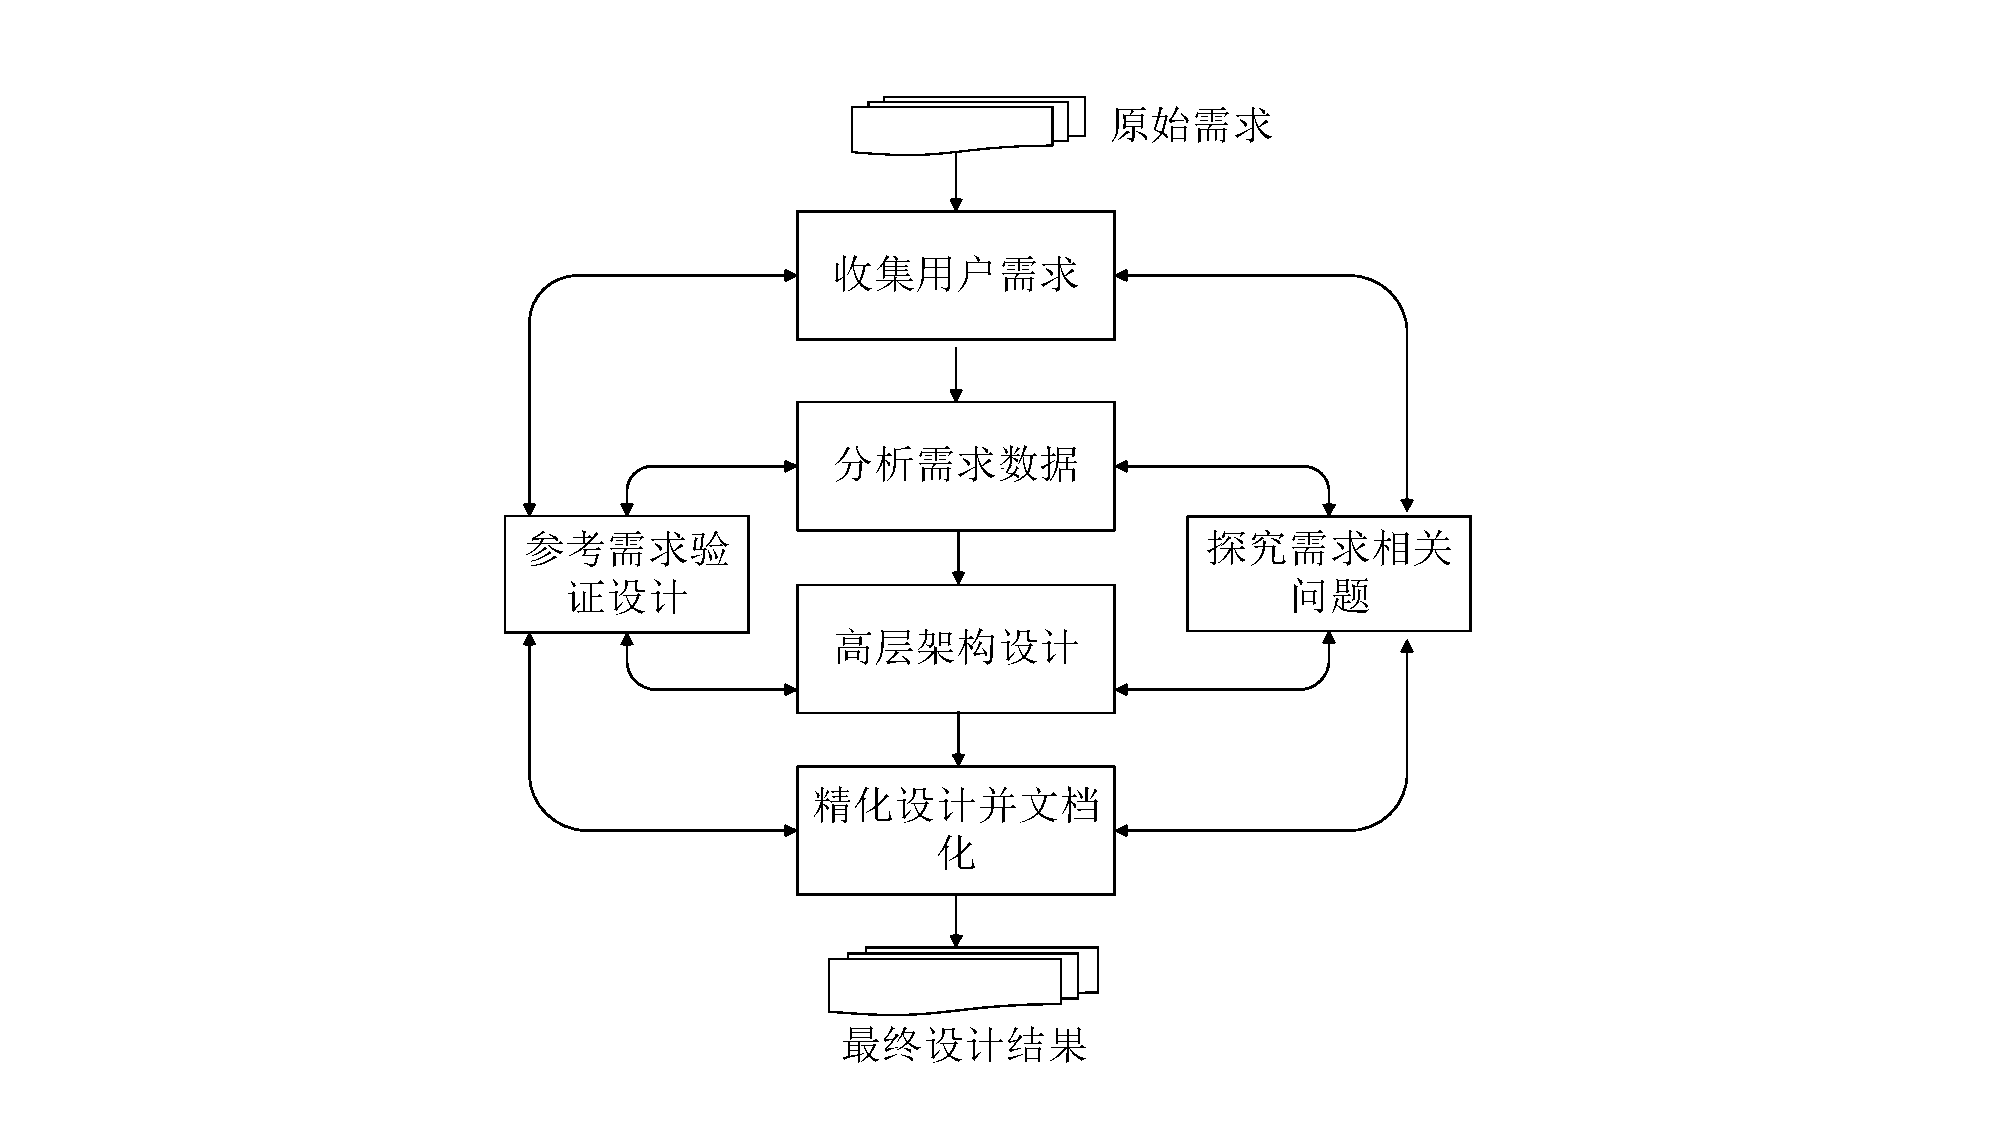
\includegraphics[width=0.5\textwidth]{images/PSP设计过程.pdf}
    \vspace{-1em}
\end{figure}

\subsubsection{设计什么?}
\vspace{-0.8em}
\begin{multicols}{2}
    \begin{enumerate}[label=\arabic*.]
        \item 设计目标程序在整个应用系统中的位置
        \item 设计目标程序的使用方式
        \item 设计目标程序与其他组件以及模块之间的关系
        \item 设计目标程序外部可见的变量和方法
        \item 设计目标程序内部运作机制
        \item 设计目标程序内部静态逻辑
    \end{enumerate}
\end{multicols}
\vspace{-1em}

\subsubsection{设计内容}
\vspace{-0.5em}
\begin{table}[H]
    \centering
    \begin{tabular}{|c|c|c|}
    \hline
                  & \textbf{动态信息} & \textbf{静态信息}  \\ \hline
    \textbf{外部信息} & 交互信息(服务、消息等)  & 功能(继承、类结构等)    \\ \hline
    \textbf{内部信息} & 行为信息(状态机)     & 结构信息(属性、业务逻辑等) \\ \hline
    \end{tabular}
\end{table}
\vspace{-1em}

\subsubsection{设计模板}
\begin{wraptable}{r}{6cm}
    \centering
    \vspace{-1em}
    \resizebox{6cm}{!}{\begin{tabular}{|c|c|c|}
        \hline
                      & \textbf{动态信息} & \textbf{静态信息} \\ \hline
        \textbf{外部信息} & OST/FST       & FST           \\ \hline
        \textbf{内部信息} & SST           & LST           \\ \hline
    \end{tabular}}
    \caption*{PSP设计模板展现的信息}
    \vspace{-1.5em}
\end{wraptable}
PSP设计模板
\begin{itemize}
    \item 操作规格模板(Operational Specification Template, OST)
    \item 功能规格模板(Functional Specification Template, FST)
    \item 状态规格模板(State Specification Template, SST)
    \item 逻辑规格模板(Logical Specification Template, LST)
\end{itemize}


\paragraph{操作规格模板OST}~{} \par
\begin{itemize}
    \item 描述系统与外界的交互,用于场景描述:也就是用户与待设计系统的正常情况和异常情况下的交互
    \item 定义测试场景和测试用例,用来与用户讨论需求的基础,特别是操作相关的需求描述
    \item 与UML比较:用例图、时序图
\end{itemize}

\paragraph{功能规格模板FST}~{} \par
\vspace{-0.8em}
\begin{multicols}{2}
    \begin{itemize}
        \item 描述系统的对外接口,是一种静态信息的展现
        \item 提供的典型信息有类和继承关系、外部可见的属性和方法等
        \item 用形式化符号等方法描述方法等行为,消除二义性
        \item 与UML对比:UML类图,但类图的方法的行为没有描述
    \end{itemize}
\end{multicols}
\vspace{-1em}

\paragraph{状态规格模板SST}~{} \par
可以精确定义程序的所有状态、状态之间的转换以及伴随着每次状态转换的动作

SST模板中,需要描述如下的信息
\vspace{-0.8em}
\begin{multicols}{3}
    \begin{itemize}
        \item 所有状态的名称
        \item 所有状态的简要描述
        \item 在 SST 中需要使用的参数和方法的名称与描述
        \item 状态转换的条件
        \item 状态转换是发生的动作
    \end{itemize}
\end{multicols}
\vspace{-1em}

与UML对比:UML状态图

\paragraph{逻辑规格模板LST}~{} \par
可以精确描述系统的内部静态逻辑。为了消除描述的二义性,一般建议使用伪代码配合形式化符号来描述设计结果

LST模板中,需要描述如下的信息
\vspace{-0.8em}
\begin{multicols}{2}
    \begin{itemize}
        \item 关键方法的静态逻辑
        \item 方法的调用
        \item 外部引用
        \item 关键数据的类型和定义
    \end{itemize}
\end{multicols}
\vspace{-1em}

与UML对比:没有对应图

\paragraph{UML}~{} \par
\begin{itemize}
    \item UML图有用例图、时序图、类图、状态机图
    \item UML的用例图和时序图提供了与PSP中OST同样的信息
    \item UML中的时序图和类图所描述的类之间的关系以及对象之间的交互信息在PSP的4个设计模板中没有对应的内容
    \item UML类图中记录了方法的型构,然而方法的行为没有描述,这一点在PSP的FST中有相应的内容
    \item PSP中的LST用以描述程序的静态逻辑,这在UML没有对应的图示方法
    \item UML中的状态图与SST描述的状态图类似,但是SST中描述的关于状态、状态转换条件以及状态转换中的动作没有对应的UML图示方法
\end{itemize}

\paragraph{考试题目}~{} \par
\begin{problem}
请解释设计的层次的概念和意义,并解释如何将PSP的4个设计模版应用在不同的设计层次之中?
\begin{figure}[H]
    \vspace{-0.5em}
	\centering
	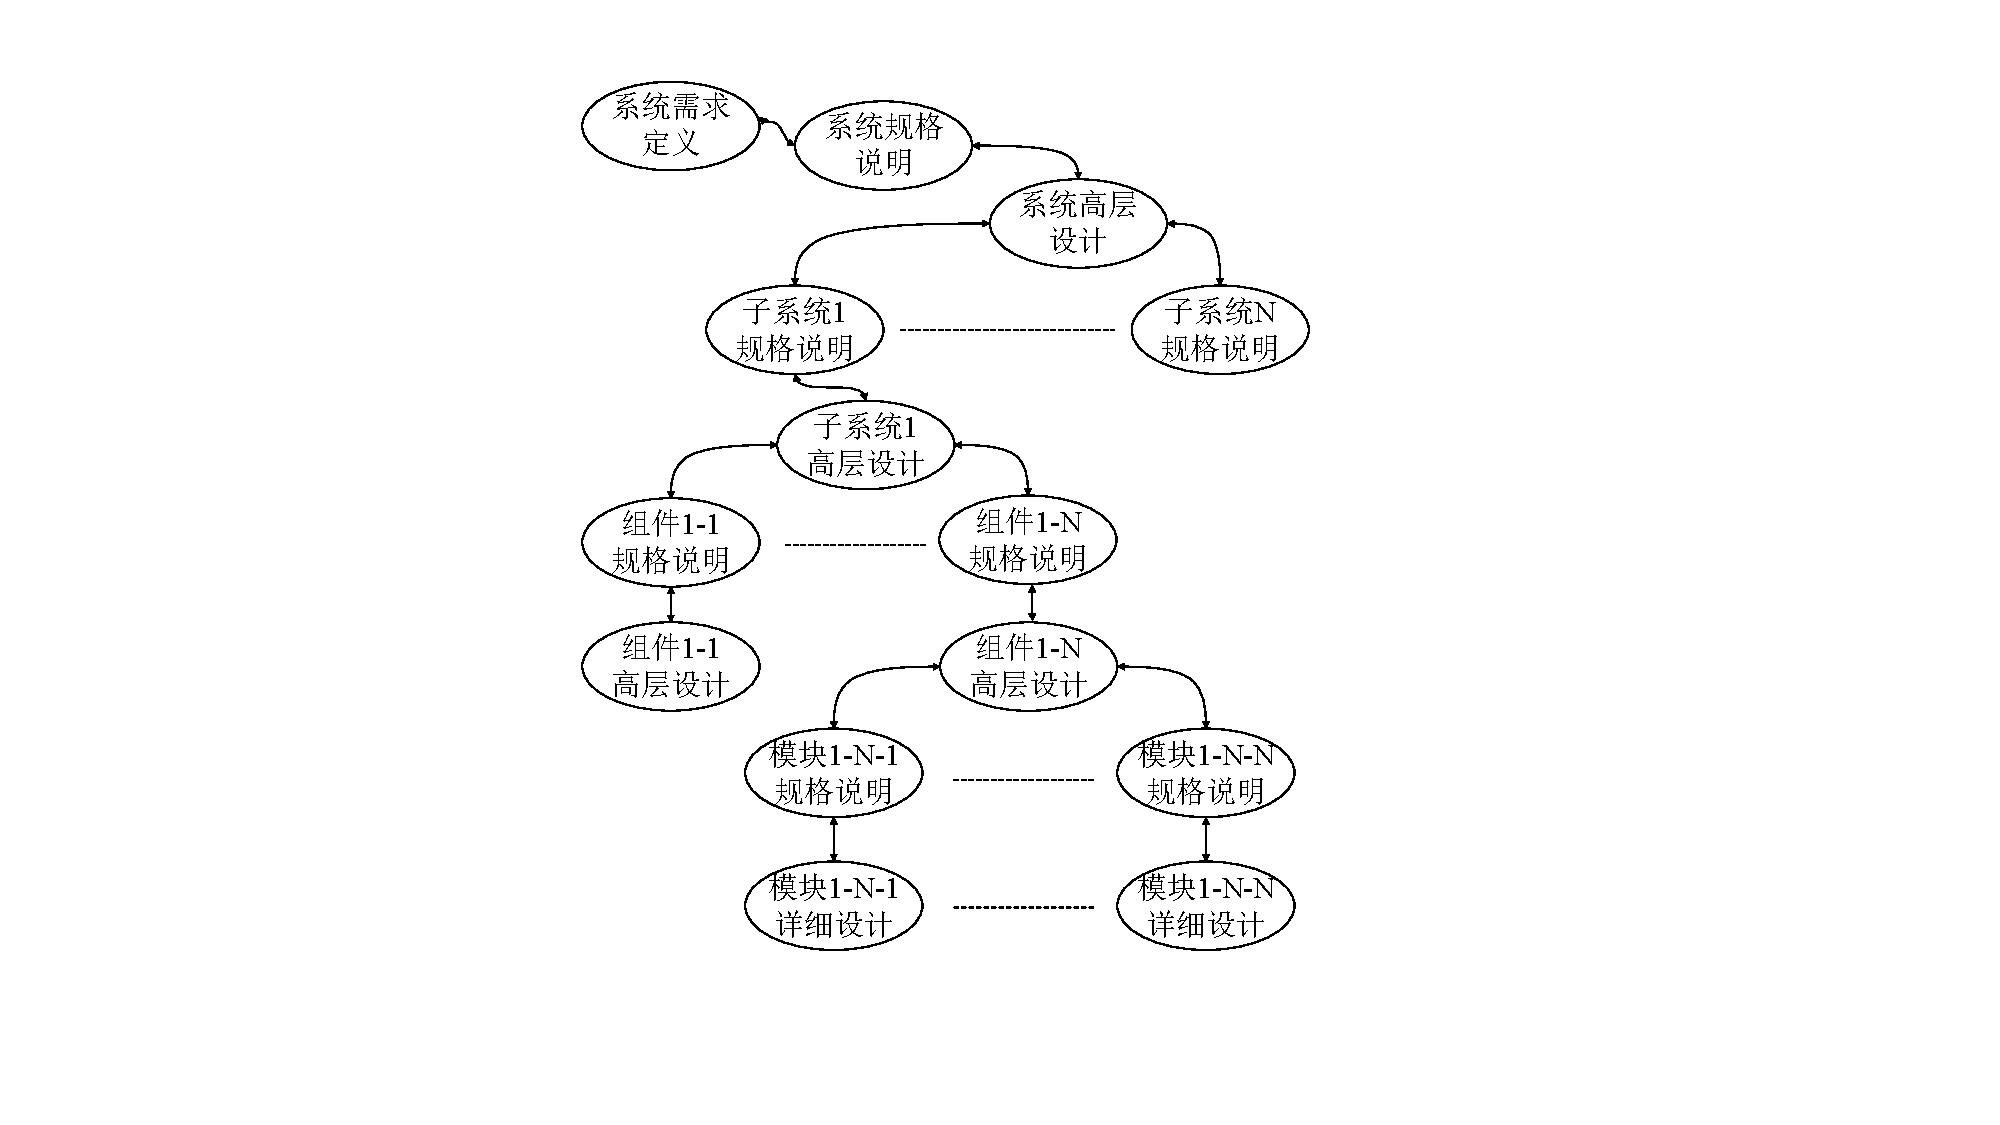
\includegraphics[width=0.47\textwidth]{images/设计的层次.pdf}
    \vspace{-1em}
\end{figure}
\end{problem}

\subsubsection{PSP设计验证方法}
意义:简单评审不足以发现复杂缺陷

\paragraph{状态机验证}~{} \par
检查状态机的完整性和正交性
\begin{itemize}
    \item 完整性:对于状态机中任何一个状态,对应的所有条件组合,下一个状态的转换都有定义
    \item 正交性:对于状态机中任何一个状态,其所有下一个状态的转换条件都不能相同
\end{itemize}

验证步骤:
\vspace{-0.8em}
\begin{multicols}{2}
    \begin{enumerate}[label=\arabic*.]
        \item 检查状态机,消除死循环和陷阱状态
        \item 检查状态转换,验证完整性和正交性
        \item 评价状态机,检验是否体现设计意图
    \end{enumerate}
\end{multicols}
\vspace{-1em}

示例:使用状态图,检查死循环和陷阱状态;使用真值表来进行分析
\begin{figure}[H]
    \vspace{-0.5em}
	\centering
	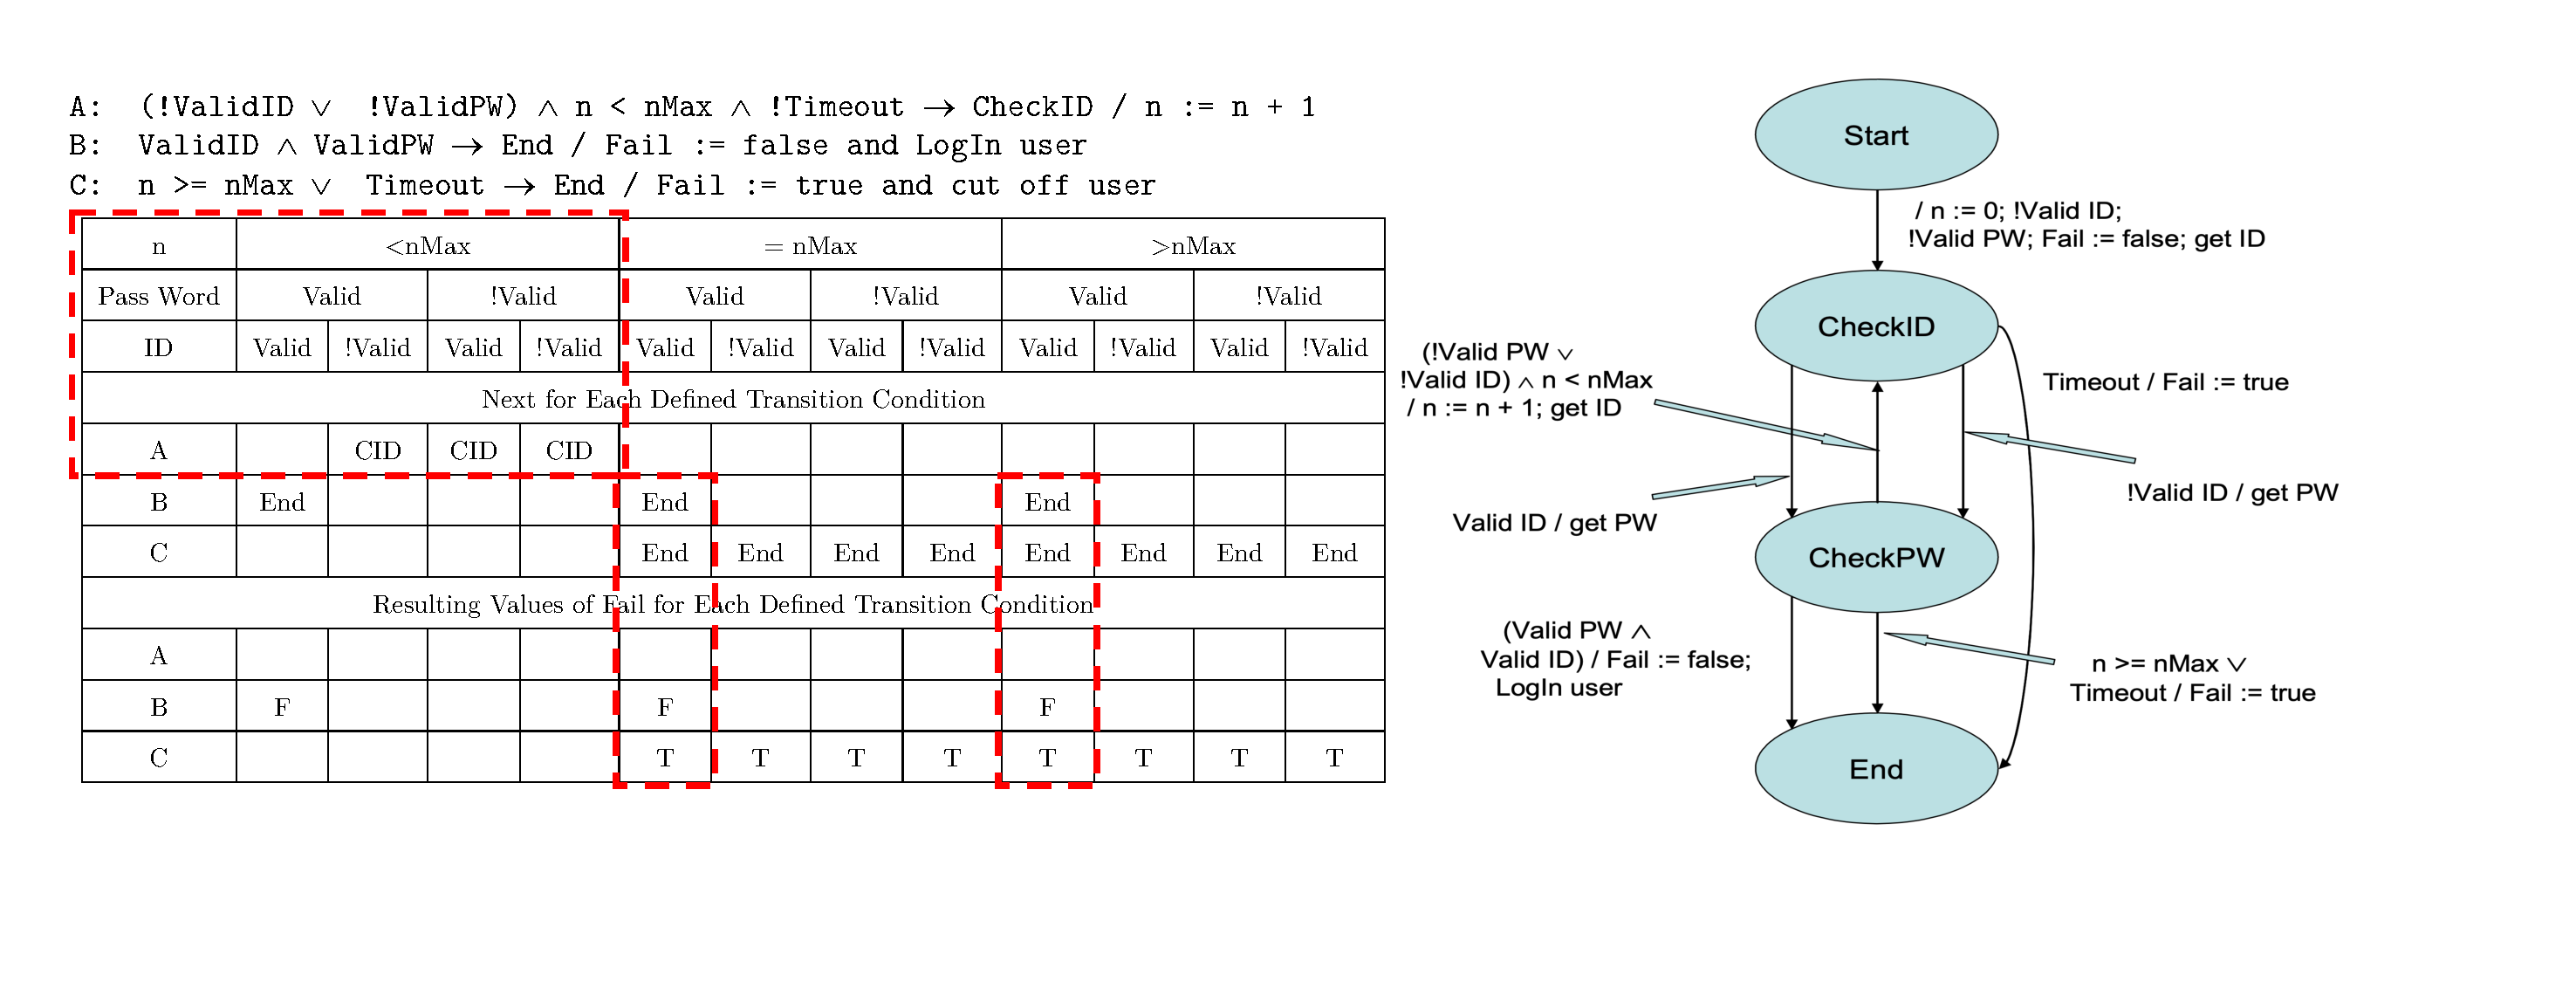
\includegraphics[width=\textwidth]{images/状态机示例.pdf}
    \vspace{-3em}
\end{figure}

\paragraph{符号化验证}~{} \par
将描述设计的逻辑规格(一般用伪代码程序表示)用代数符号来表示,然后系统地开展分析和验证

验证步骤:
\vspace{-0.8em}
\begin{multicols}{2}
    \begin{enumerate}[label=\arabic*.]
        \item 识别伪码程序中的关键变量
        \item 将这些变量使用代数符号表示,重写伪码程序
        \item 分析伪码程序的行为
    \end{enumerate}
\end{multicols}
\vspace{-1em}

示例:交换两个变量的值
\begin{figure}[H]
    \vspace{-0.5em}
	\centering
	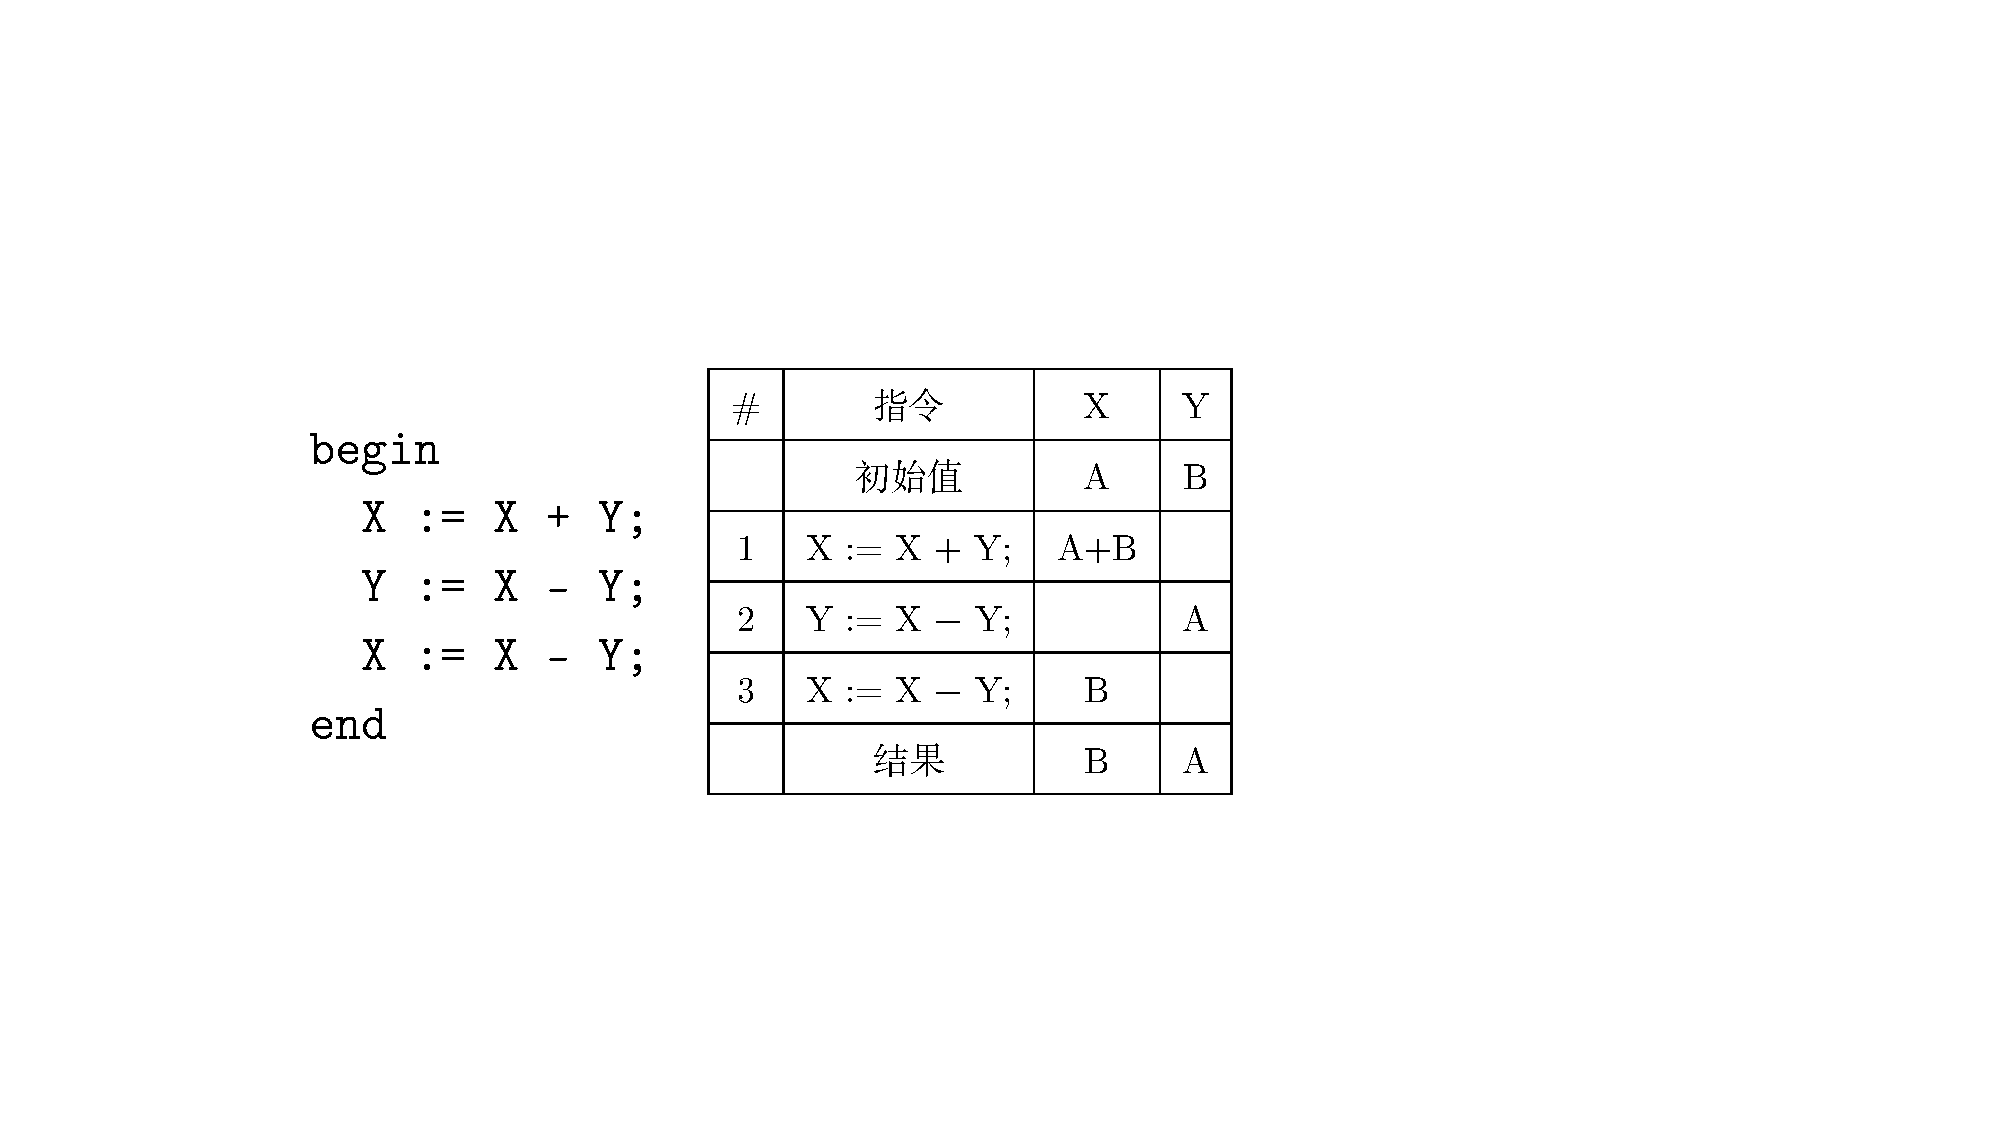
\includegraphics[width=0.5\textwidth]{images/符号化执行验证示例.pdf}
    \vspace{-1em}
\end{figure}

\vspace{-0.5em}
\begin{spacing}{1.2}
    \centering
    \begin{longtable}{|m{7.2cm}|m{7.2cm}|}
        \hline
        \multicolumn{1}{|c|}{\textbf{优点}} & \multicolumn{1}{c|}{\textbf{缺点}} \\ \hline
        \vspace{-1em}
        \begin{enumerate}[label=\arabic*.,leftmargin=1em]
            \item 实施简单,可以给出一般化的验证结果
            \item 适用于不复杂的算法,特别是遗漏系统的改造中,应用这种方法识别和理解原有的设计
            \vspace{-1.3em}
        \end{enumerate}
        & 不适合于有复杂逻辑的场合;纯手工验证方法容易引入错误
        \\ \hline
    \end{longtable}
	\end{spacing}
\vspace{-1em}

\paragraph{执行表验证}~{} \par
步骤:
\vspace{-0.8em}
\begin{multicols}{2}
    \begin{enumerate}[label=\arabic*.]
        \item 识别伪码程序的关键变量
        \item 构建表格,表格左侧填入主要程序步骤,右侧填入关键变量
        \item 初始化被选定的变量
        \item 跟踪被选择的关键变量的变化情况,从而判断程序行为
    \end{enumerate}
\end{multicols}
\vspace{-1em}

优点:实施简单;结果可靠,可用于复杂逻辑的验证

缺点:每次只能验证一个用例;手工验证比较耗时,容易引入错误

\paragraph{跟踪表验证}~{} \par
步骤:
\vspace{-0.8em}
\begin{multicols}{2}
    \begin{enumerate}[label=\arabic*.]
        \item 识别伪码程序的关键变量
        \item 构建表格,表格左侧填入主要程序步骤,右侧填入关键变量
        \item 初始化被选定的变量
        \item 识别将伪码程序符号化的机会,并加以符号化
        \item 定义并且优化用例组合
        \item 跟踪被选择的关键变量的变化情况,从而判断程序行动
    \end{enumerate}
\end{multicols}
\vspace{-1em}

跟踪表应用符号化以及用例识别等方法,对程序的一般化行为进行验证,是执行表验证的补充,可以每次验证多个用例,从而提供更加高效地开展验证工作

\paragraph{正确性验证}~{} \par
将伪码程序当做数字定理,采用形式化方法加以推理和验证

步骤:
\vspace{-0.8em}
\begin{multicols}{2}
    \begin{enumerate}[label=\arabic*.]
        \item 分析和识别用例
        \item 对于复杂伪码程序的结构,应用正确性验证的标准问题逐项加以验证
        \item 对于不能明确判断的复杂程序结果,使用跟踪表等辅助验证
    \end{enumerate}
\end{multicols}
\vspace{-1em}

While-Do循环的验证
\begin{enumerate}[label=\arabic*.]
    \item 条件1:condition 是否最终一定会为“假”,从而使得循环可以结束。
    \item 条件2:condition 为“真”的时候,单独的循环结构执行结果与循环体再加一个循环结构,其执行结果是否一致?
    \item 条件3:condition 为“假”的时候,循环体内所有变量是否未被修改?
\end{enumerate}

	\section{TSP团队软件过程}
TSP提供了
\vspace{-0.8em}
\begin{multicols}{3}
    \begin{itemize}
        \item 一个已定义的团队构建过程
        \item 一个团队作业框架
        \item 一个有效的管理环境
    \end{itemize}
\end{multicols}
\vspace{-1em}

\subsection{团队工程开发:需求开发}
需求开发包含需求获取、需求汇总、需求验证

\subsubsection{需求分类}
\textbf{客户需求}描述的是客户的期望,是客户解决问题的愿望
\begin{itemize}
    \item 客户需求可能很简单,也可能很复杂;可能很清晰,也可能模糊
    \item 比如,客户希望有一种快速进行数据计算的工具帮助其完成繁琐的计算工作
\end{itemize}

\textbf{产品需求}描述的是开发团队所提供的解决方案。即针对上述的客户需求,开发团队设计出一个可以帮助客户解决工作当中碰到的问题的方案。

\textbf{产品组件}需求描述的是组成产品的各个组件的需求规格。与产品需求相比,这是更低层次,更为细致的描述了上述解决方案中的某个组件的功能、性能与形式等。

\subsubsection{为什么说“需求是一切工程活动的基础”}
\begin{itemize}
    \item 设计活动一定是依据需求而开展的
    \item 产品集成活动中,各个组件之间的接口必须满足事先确定的接口需求,否则会造成接口不匹配
    \begin{itemize}
        \item 验证(Verification)活动也是检验获得的产品和产品组件能不能满足各自事先定义好的需求规格
        \item 确认(Validation)活动是为了确保产品可以满足客户的需求以及实际操作场景的要求
    \end{itemize}
    \item 此外,需求也是项目计划活动的关键输入。比如,项目的规模估算、成本估算等必须参考需求来进行
\end{itemize}

\subsubsection{需求获取}
需求是采用“诱导”式方法获取客户的显式需求和隐式需求,尽可能的识别客户的期望与所受到的限制
\begin{itemize}
    \item “诱导”不仅仅是普通的需求采集,隐含了更加积极地、前瞻性地识别那些客户没有明确提供的额外需求
    \item 客户所受到的限制也应当作为需求开发过后需要关注的内容。限制包括技术、成本、时间、风险、行业规则、法律等等
\end{itemize}

\subsubsection{需求汇总}
\begin{itemize}
    \item 整理各种来源的信息,识别缺失的信息
    \item 解决冲突的需求
    \begin{itemize}
        \item 需求的整理和转化:我们需要将客户的需求转换为产品需求和产品组件的需求
        \item 推导未显式描述的需求内容,例如采用某项技术的附属需求
    \end{itemize}
\end{itemize}

\subsubsection{需求验证}
对需求进行分析和确认,以确保符合使用者预期,典型活动包括:
\begin{itemize}
    \item 建立和维护操作概念和相关的场景;场景一般而言是指使用产品时可能发生的时间顺序
    \item 分析需求,以确保其必要性、充分性和平衡性
    \item 确认需求,以确保将要产生的产品能在预期的用户环境中运行并且工作正常
\end{itemize}

\subsubsection{需求文档制作}
需求开发工作完成的一个基本标志是形成了一份完整的、规范的、经过评审的需求规格说明书

需求规格说明书的编制是为了使用户和软件开发者双方对该软件的初始规定有一个共同的理解,使之成为整个开发工作的基础

\paragraph{优秀需求规格文档特征}~{} \par
\vspace{-0.5em}
\begin{spacing}{1.2}
    \centering
    \begin{longtable}{|m{2cm}<{\centering}|m{13cm}|}
        \hline
        \textbf{特征} & \multicolumn{1}{c|}{\textbf{描述}}                                                         \\ \hline
        内聚特征        & 需求规格描述应当尽可能内聚,即仅仅用以说明一件事情                                                                \\ \hline
        完整特征        & 需求规格描述应当完整,不能遗漏信息                                                                        \\ \hline
        一致特征        & 需求规格描述的各个条目和章节不能互相矛盾,需求规格描述与所有外部的参考资料之间也应当消除矛盾之处                                         \\ \hline
        原子特征        & 需求规格描述的过程中,应当尽可能避免连接词的使用。如果需要描述多项内容,可以分别用简单语句加以描述                                        \\ \hline
        可跟踪特征       & 客户需求、产品需求以及产品组件需求必须可以双向跟踪,即客户需求的任何内容,都应当在产品需求和产品组件需求中得到体现。反之,产品组件需求的每一项描述也要可以跟踪到客户需求中的内容 \\ \hline
        非过期特征       & 需求描述的内容必须体现相关干系人对于项目的最新认识。即不能包含已经废弃的需求定义                                                 \\ \hline
        可行性特征       & 需求规格描述的各项内容应该在项目所拥有的资源范围内可以实现                                                            \\ \hline
        强制特征        & 需求规格描述的内容应当体现强制性,即需求规格描述的内容的任何一项缺失,都会导致最终产品不能满足客户期望。因此,可选的需求内容要么不要出现,要么以明确的方式标注          \\ \hline
        可验证特征       & 需求规格描述应当便于在后期开发过程中进行验证。即实现该需求与否,应该有明确的判断标准                                               \\ \hline
    \end{longtable}
\end{spacing}
\vspace{-1em}

\paragraph{SRS示例}~{} \par
\vspace{-0.8em}
\begin{multicols}{5}
    \begin{enumerate}[label=\arabic*.]
        \item 引言
        \item 系统定义
        \item 应用环境
        \item 功能规格
        \item 性能需求
        \item 实现约束
        \item 质量描述
        \item 其它要求
        \item 参考材料
        \item 签字认证
    \end{enumerate}
\end{multicols}
\vspace{-1em}

对于需求规格模板中的功能规格定义可以用多种方式灵活定义。典型的方式有原型描述、结构化分析方法描述、用例描述、可测试需求列表描述等

\subsubsection{考试题目}
\begin{problem}
请解释需求开发中客户需求和产品需求的差别,并设计一个流程来完成需求开发工作
\end{problem}

\begin{problem}
请给出需求开发的完整过程,并且解释客户需求和产品需求的各自含义以及在需求开发过程中该如何体现客户需求和产品需求
\end{problem}

\subsection{团队工程开发:团队设计}

\subsubsection{团队智慧}
发挥团队智慧两大挑战:
\vspace{-0.8em}
\begin{multicols}{2}
    \begin{itemize}
        \item 确定整体架构之前很难进行分工
        \item 鼓励团队成员在讨论和评审会议中的参与程度
    \end{itemize}
\end{multicols}
\vspace{-1em}

\subsubsection{设计标准}
\begin{itemize}
    \item 命名规范:项目小组应当设计一个统一的命名规范来命名各个模块并建立系统词典
    \item 接口标准:组件之间的接口标准和格式也需要作为设计标准的内容之一加以定义
    \item 系统出错信息:系统异常信息和出错信息往往也需要通过一个规范加以标准化
    \item 设计表示标准:设计表示标准定义了设计工作的产物应当满足的标准
\end{itemize}

\subsubsection{复用性支持}
在设计阶段必须要充分考虑复用的可能。为了支持复用,软件项目团队需要建立一套复用管理流程,具体而言,包括:
\vspace{-0.8em}
\begin{multicols}{3}
    \begin{itemize}
        \item 复用接口标准
        \item 复用文档标准
        \item 复用质量保证机制
    \end{itemize}
\end{multicols}
\vspace{-1em}

\subsubsection{可测试性考虑}
设计可测试性考虑主要体现在两方面:
\vspace{-0.8em}
\begin{multicols}{2}
    \begin{itemize}
        \item 要尽可能减少测试代码的数量
        \item 要制作合理的测试计划
    \end{itemize}
\end{multicols}
\vspace{-1em}

\subsubsection{可用性考虑}
\begin{itemize}
    \item 可用性的问题应当在设计阶段就开始考虑,而不能推延到实现阶段
    \item 针对每一个关键功能都定义操作概念和操作场景
    \item 分析操作场景以确保软件系统开发完成之后,系统使用者会满意
    \item 必要时,可以邀请最终用户参与场景的评审,使用模拟、原型等技术,更好的把握用户真实意图
\end{itemize}

\subsubsection{设计的文档化}
\vspace{-0.8em}
\begin{multicols}{3}
    \begin{enumerate}[label=\arabic*.]
        \item 引言
        \item 设计文档目的
        \item 问题陈述
        \item 团队信息
        \item 高层设计
        \begin{enumerate}[label=\alph*.]
            \item 系统架构
            \item 组件分配表
            \item 功能规格说明
            \item 操作场景
            \item 各个模块工作方式的伪码描述
            \item 用户界面
        \end{enumerate}
        \item 详细设计
        \begin{enumerate}[label=\alph*.]
            \item 状态机设计
            \item 模块内部工作方式的伪码描述   
        \end{enumerate}
        \item 限制条件
        \begin{enumerate}[label=\alph*.]
            \item 标准兼容
            \item 硬件限制
            \item 开发限制   
        \end{enumerate}
        \item 参考材料
    \end{enumerate}
\end{multicols}
\vspace{-1em}

\subsection{团队工程开发:实现策略}

\subsubsection{评审的考虑}
\begin{itemize}
    \item 设计的时候采用的策略是自顶向下、逐层精化,这有利于建立系统的整体观
    \item 实现的时候为了方便对实现结果评审,建议采用自底向上的方式进行,首先实现底层的内容,然后对这些底层的模块进行评审,有利于复用策略的应用
\end{itemize}

\subsubsection{复用策略}
采用自底向上的开发策略有利于进行复用,几个经典的复用策略:
\begin{itemize}
    \item \textbf{编码注释的应用}:编码注释采用统一格式,标明功能,调用方式。异常信息等有利于复用的信息
    \item \textbf{站立式会议}:在会上,团队成员可以讨论实现计划,识别可复用组件,了解现有的复用组件库的内容
\end{itemize}

\subsubsection{可测试性考虑}
实现计划必须与测试计划一致,不能出现集体测试的时候部分模块未实现的情况

\subsection{团队工程开发:集成策略选择}
\vspace{-0.5em}
\begin{spacing}{1.2}
    \centering
    \begin{longtable}{|m{2cm}<{\centering}|m{4.1cm}|m{4.1cm}|m{4.1cm}|}
        \hline
        \textbf{策略名} & \multicolumn{1}{c|}{\textbf{特点}}                               & \multicolumn{1}{c|}{\textbf{优点}}            & \multicolumn{1}{c|}{\textbf{缺点}}                                   \\ \hline
        大爆炸集成策略      & 将所有已经完成的组件放在一起进行一次集成                                           & 需要很少的测试用例                                   & 需要所有有待集成的组件质量非常高,否则会出现难以定位缺陷位置的问题,从而消耗很多测试时间;另外,系统越复杂,规模越大,问题越突出   \\ \hline
        逐一添加集成策略     & 与大爆炸集成策略相反,采取一次添加一个组件的方式进行集成                                   & 很容易定位缺陷位置,特别是在产品组件质量不高的情况下,每次集成之前都有着坚实的质量基础 & 需要测试用例非常多;存在有大量的回归测试,测试时间成本大                                       \\ \hline
        集簇集成策略       & 是对逐一添加集成策略的改进,把有相似功能或者有关联的模块优先进行集成,形成可以工作的组件,然后以组件为单位继续较高层次的集成 & 可以尽早获得一些可以工作的组件,有利于其它组件测试工作的开展              & 过于关注个别组件,而缺乏系统的整体观,不能尽早发现系统层面的缺陷                                   \\ \hline
        扁平化集成策略      & 优先集成高层的部件,然后逐步将各个组件、模块的真正实现加入系统。即尽快构建一个可以工作的扁平化系统              & 可以尽早发现系统层面的缺陷                               & 为了确保完成的系统,需要大量的打“桩”(stub),即提供一些直接提供返回值的伪实现。这种方式往往不能覆盖整个系统应该处理的多种状态 \\ \hline
    \end{longtable}
\end{spacing}
\vspace{-1em}


\subsubsection{考试题目}
\begin{problem}
产品组件集成策略有哪些?请解释这些策略的优缺点。在此基础上,解释如果要实现高质量集成,可能需要注意哪些方面。
\end{problem}

\begin{problem}
请罗列集成测试的典型策略,并且解释各个集成测试策略的优缺点?
\end{problem}

\subsection{团队工程开发:验证与确认V\&V}

\subsubsection{什么是V\&V}
\begin{itemize}
    \item 验证(Verification)活动也是检验获得的产品和产品组件能不能满足各自事先定义好的需求规格
    \item 确认(Validation)活动是为了确保产品可以满足客户的需求以及实际操作场景的要求
    \item 验证(Verification)和确认(Validation)都是为了提升最终产品的质量而采取的措施
\end{itemize}

\subsubsection{V\&V的区别与联系}
验证和确认的目的不同:
\begin{itemize}
    \item 验证是目的是确保选定的工作产品与事先指定给该工作产品的需求(即产品需求或产品组件需求)一致
    \item 确认的目的则是确保开发完成的产品或者产品组件在即将要使用该产品或者产品组件的环境中工作正确,关注的是客户需求的满足
\end{itemize}

验证和确认又是相互依存、关系紧密的两个活动
\begin{itemize}
    \item 验证活动的依据来源于确认的目标,即产品组件需求必须与客户需求一致
    \item 验证活动为确认活动提供了前提条件,在完成产品需求和产品组件需求之前,考虑客户需求是否满足是没有意义的
\end{itemize}

\subsubsection{V\&V的活动}
\vspace{-0.5em}
\begin{spacing}{1.2}
    \centering
    \begin{longtable}{|m{1.5cm}<{\centering}|m{13.8cm}|}
        \hline
        \textbf{活动} & \multicolumn{1}{c|}{\textbf{说明}} \\ \hline
        环境准备 & 
        \vspace{-1.1em}
        \begin{enumerate}[label=,leftmargin=0em]
            \item 对于验证工作,如果是评审,则需要准备文件材料、人员以及会议场所等;如果是测试,需要准备模拟器、场景生成程序、环境控制以及其他系统接口等
            \item 对于确认工作,则需要模拟真实环境和场景
        \vspace{-1.3em}
        \end{enumerate}
        \\ \hline
        对象选择 & 
        \vspace{-1.1em}
        \begin{enumerate}[label=,leftmargin=0em]
            \item 对于验证工作,验证对象往往从工作产品中选择
            \item 对于确认工作,确认对象从产品中选择
        \vspace{-1.3em}
        \end{enumerate}
        \\ \hline
        活动实施 & 
        \vspace{-1.1em}
        \begin{enumerate}[label=,leftmargin=0em]
            \item 确认工作活动包括早期对产品需求评审工作和最后的验收测试
            \item 验证工作:一般的评审和测试工作
        \vspace{-1.3em}
        \end{enumerate}
        \\ \hline
        结果分析 &
        \vspace{-1.1em}
        \begin{enumerate}[label=,leftmargin=0em]
            \item 对于评审结果,可以根据评审结果反思软件开发过程的合理性、以及是否还有隐藏的缺陷
            \item 对于验收测试的结果,则可以关注那些一直遗留到验收阶段才被发现的缺陷,看看这些缺陷在什么阶段被引入,为什么前面未能发现等
        \vspace{-1.3em}
        \end{enumerate} 
        \\ \hline
    \end{longtable}
\end{spacing}
\vspace{-1em}


\subsubsection{V\&V的例子}
\vspace{-0.8em}
\begin{multicols}{4}
    \begin{itemize}
        \item 单元测试:验证
        \item 集成:验证
        \item 需求评审:确认
        \item 验收测试:确认
    \end{itemize}
\end{multicols}
\vspace{-1em}

\subsubsection{考试题目}
\begin{problem}
请解释在质量保障活动中的V\&V分别是什么含义?两者之间的关系是什么?
\end{problem}

\begin{problem}
请举例说明验证和确认的区别和联系? 
\end{problem}

\subsection{团队项目规划:工作分解结构与范围管理}

\subsubsection{工作分解结构}
工作分解结构(WBS, Work Breakdown Structure)是以可交付成果为导向对满足项目目标和开发交付产物的项目相关工作进行的分解
\vspace{-0.8em}
\begin{multicols}{2}
    \begin{itemize}
        \item 它归纳和定义了项目的整个工作范围
        \item 每下降一层代表对项目工作的更详细定义
    \end{itemize}
\end{multicols}
\vspace{-1em}

作用/特点:
\begin{itemize}
    \item 提供了\textbf{项目范围基线},是范围变更的重要输入
    \item 可以展现\textbf{项目整体观},使得项目团队成员可以集中注意力实现项目的目标上
    \item 为开发项目提供了一个整体框架,\textbf{防止遗漏}项目的可交付成果
    \item 使得项目中各个角色的责任更明确,帮助项目团队的建立和获得项目成员的承诺
    \item 为评估和分配任务提供具体的工作包的定义,工作包可以分配给项目某个成员或者另一个团队
    \item 是进行估算和编制项目日程计划的基础
    \item 可以帮助项目团队理解工作内容,分析项目的风险
\end{itemize}

表示方式:树型层次结构;清单型层次结构

\paragraph{创建WBS}~{} \par
将复杂的项目逐步分解为一系列明确定义的工作任务并作为随后计划活动的指导文档

要将整个项目分解成工作包:
\vspace{-0.8em}
\begin{multicols}{2}
    \begin{enumerate}[label=\arabic*.]
        \item 识别和分析可交付成果以及相关工作
        \item 确定工作分解结构的结构与编排方法
        \item 自上而下逐层细化分解
        \item 为工作分解结构组成部分制定和分配标志编码
        \item 核实工作分解的程度是必要且充分的
    \end{enumerate}
\end{multicols}
\vspace{-1em}

\paragraph{好的WBS的检查标准}~{} \par
\begin{itemize}
    \item 最底层要素不能重复,即任何一个工作应该在WBS中的一个地方且只应该在WBS中的一个地方出现
    \item 所有要素必须清晰完整定义,即相应的数据词典必须完整定义
    \item 最底层要素必须有定义清晰的责任人,可以支持成本估算和进度安排
    \item 最底层要素是实现目标的成分必要条件,即项目的工作范围得到完整体现
\end{itemize}

\subsubsection{范围管理}
包括确保项目做且只做成功完成项目所需的全部工作的各过程,WBS为范围管理提供了基础:
\vspace{-0.8em}
\begin{multicols}{5}
    \begin{itemize}
        \item 收集需求
        \item 定义范围
        \item 创建WBS
        \item 核实范围
        \item 控制范围变更
    \end{itemize}
\end{multicols}
\vspace{-1em}

\subsection{团队项目规划:开发策略与计划}
定义:是在产品组件需求基础之上,明确每个产品组件的获得方式与顺序,从而在项目团队内部建立起大家都理解的产品开发策略

注意事项:
\vspace{-0.8em}
\begin{multicols}{3}
    \begin{itemize}
        \item WBS的使用
        \item 产品组件开发顺序的考虑
        \item 产品组件获得方式的考虑
    \end{itemize}
\end{multicols}
\vspace{-1em}

\subsection{团队项目规划:生命周期模型选择}
\begin{wraptable}{r}{0.4\textwidth}
    \centering
    \vspace{-4.5em}
    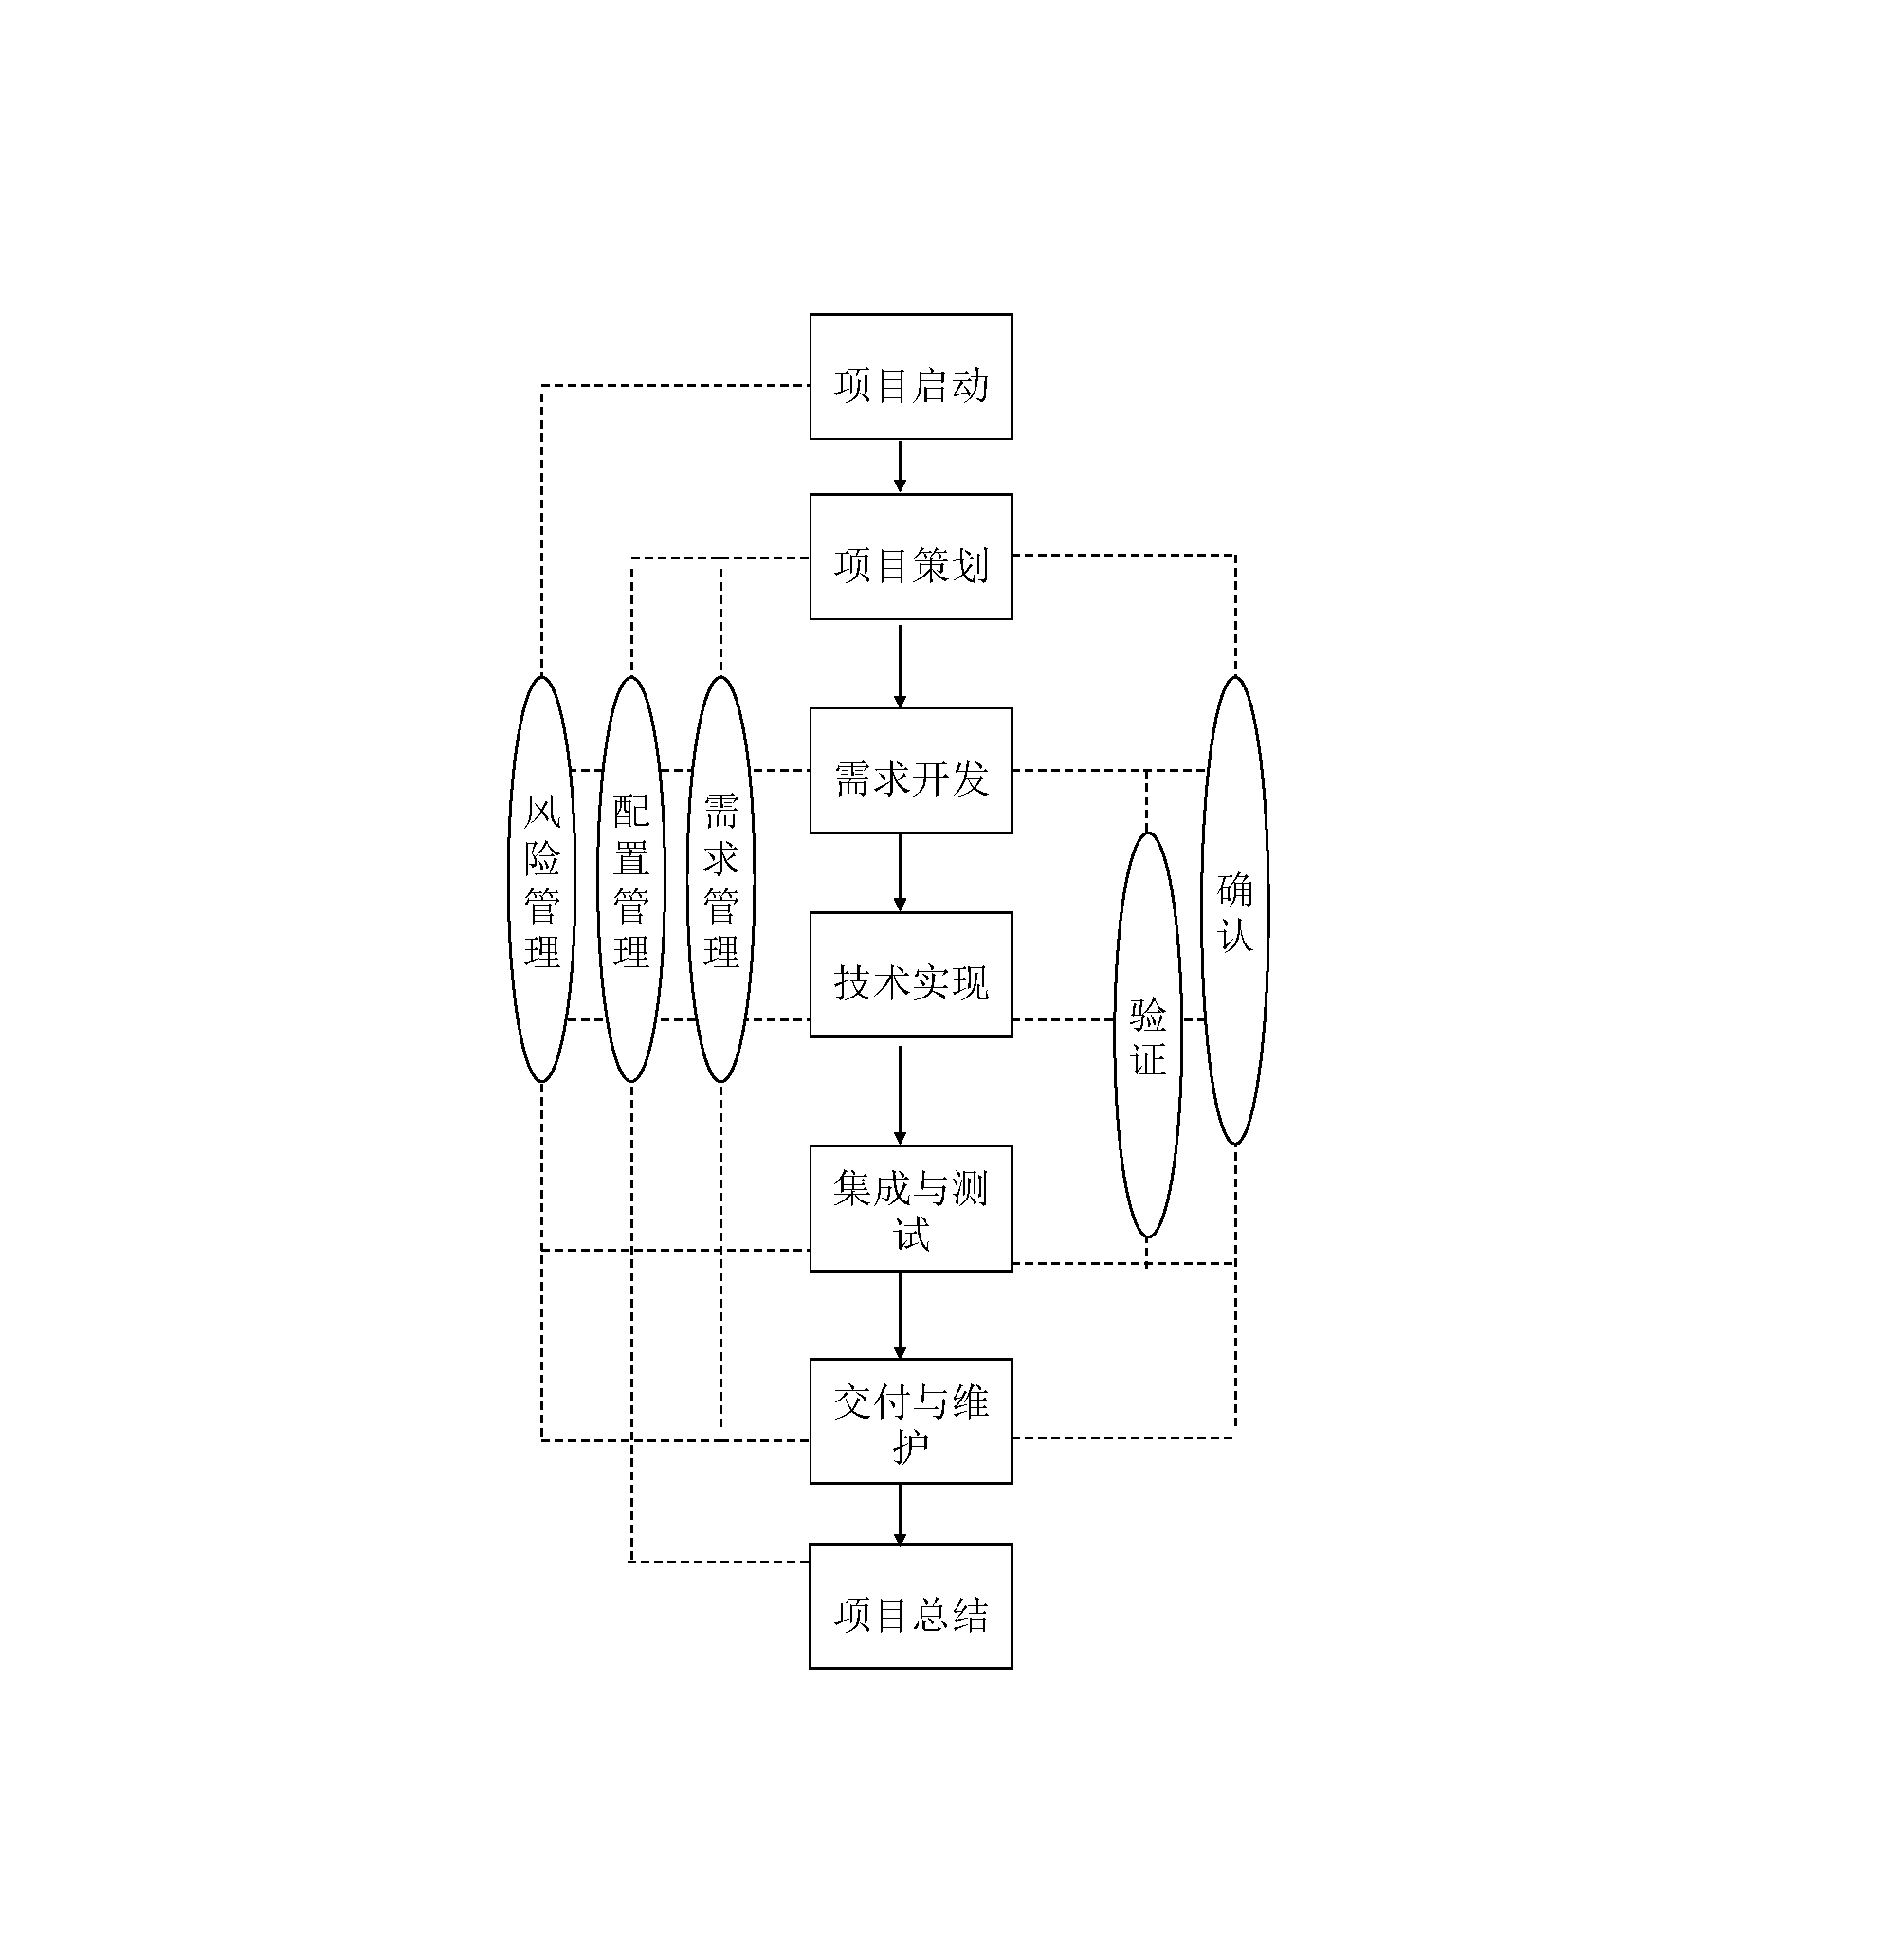
\includegraphics[width=0.32\textwidth]{images/生命周期模型.pdf}
    \vspace{-10.5em}
\end{wraptable}
生命周期模型的各个阶段
\begin{itemize}
    \item 项目启动阶段
    \item 项目策划阶段
    \item 需求开发阶段
    \item 技术实现阶段
    \item 集成与测试阶段
    \item 交付与维护阶段
    \item 项目总结
\end{itemize}

\subsection{团队项目规划:计划}

\subsubsection{日程计划原理和方法}
\paragraph{任务计划和日程计划}~{} \par
\begin{itemize}
    \item \textbf{任务计划}描述了项目所有的任务清单,任务之间的先后顺序以及每个任务所需时间资源
    \item \textbf{日程计划}描述了每个任务在日志上的安排,即每个任务计划哪天开始和计划哪天结束
    \item 制定资源计划,结合任务计划就可以定义日程计划
    \item 团队形式的日程计划考虑:
    \begin{itemize}
        \item 资源平衡:要求项目团队结合每个团队成员的工作效率、工作内容以及资源水平,找到一个时间点,让所有团队成员几乎同时完成任务
        \item 资源同步:安排日程时必须兼顾某些项目人物之间的依赖关系
    \end{itemize}
\end{itemize}

\paragraph{典型计划流程回顾}~{} \par
\vspace{-0.8em}
\begin{multicols}{3}
    \begin{itemize}
        \item 估算规模
        \item 估算资源
        \item 规划日程
    \end{itemize}
\end{multicols}
\vspace{-1em}

\subsubsection{质量计划原理和方法}
\begin{wraptable}{r}{0.55\textwidth}
    \centering
    \vspace{-4.3em}
    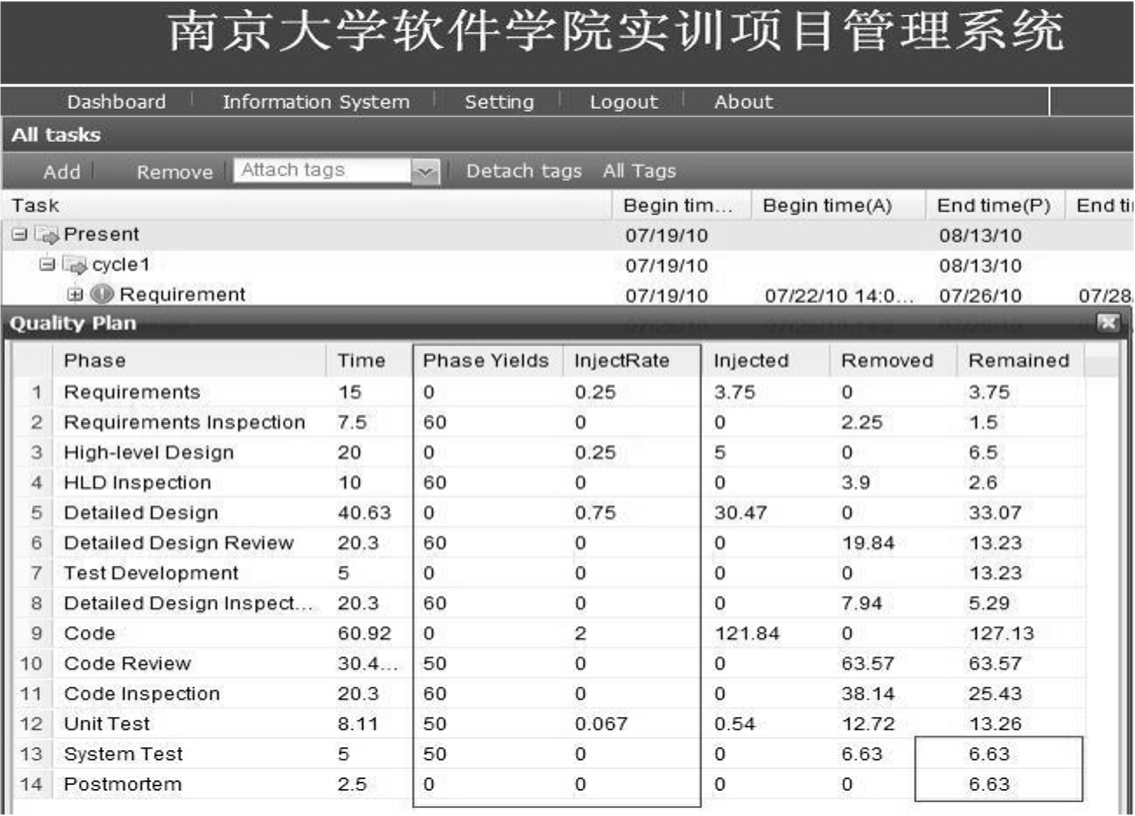
\includegraphics[width=0.55\textwidth]{images/质量计划原理和方法.png}
    \vspace{-10.5em}
\end{wraptable}
项目的质量计划中应当确定需要开展的质量保证活动
\begin{itemize}
    \item 典型的质量保证活动包括了个人评审、团队评审、单元测试、集成测试以及验收测试等
    \item 在质量计划中需要解决的关键问题是该开展哪些活动,以及这些活动开展的程度,如时间、人数和目标是什么
\end{itemize}

\subsubsection{风险计划}
风险管理的\textbf{目标}是:在风险发生前,识别出潜在的问题,以便在产品或项目的生命周期中规划和实施风险管理活动,以消除潜在问题对项目产生的负面影响

风险管理是一个持续的、前瞻的过程,此过程是项目管理的重要部分。有效的风险管理是通过相关干系人的合作与参与,尽快且积极地识别风险,指定项目风险管理计划
\begin{itemize}
    \item 风险管理需要同时考虑有关成本、进度、绩效以及其他风险的内部及外部来源
    \item 在项目初期进行变更或修正的工作负荷,通常比在项目后期来得容易、花费较低且较不具破坏性
    \item 早期且积极的风险侦测是重要的
\end{itemize}

风险管理大致分为两部分,即\textbf{风险识别}和\textbf{风险应对}

早期风险侦测的重要性:在项目初期进行变更或修正的工作负荷,通常比在项目后期来得容易、花费较低及较不具破坏性

\paragraph{风险识别}~{} \par
\begin{itemize}
    \item 风险:没有发生,有一定概率会发生,发生后有一定影响
    \item 问题:已经发生的,比如人员调动等
\end{itemize}

典型的识别方法:
\vspace{-0.8em}
\begin{multicols}{2}
    \begin{enumerate}[label=\arabic*.]
        \item 检查WBS的每个组件以找出相应的风险
        \item 使用定义好的风险分类表上来评估风险
        \item 访谈相关的领域专家
        \item 与类似项目进行比较来审查风险管理
        \item 检查以往项目的总结报告或组织级数据库
        \item 检查设计规格和协议书需求
    \end{enumerate}
\end{multicols}
\vspace{-1em}

典型的风险识别活动包括:
\vspace{-0.8em}
\begin{multicols}{2}
    \begin{enumerate}[label=\arabic*.]
        \item 识别与成本、进度及绩效相关的风险
        \item 审查可能影响项目的环境因素
        \item 审查工作分解结构的所有组件,作为风险识别的一部分,以协助确保所有的工作投入均已考虑
        \item 审查项目计划的所有组件,作为风险识别的一部分,以确保项目在各方面均已考虑
        \item 记录风险的内容、条件及可能的结果
        \item 识别每一风险相关的干系人
        \item 利用已定义的风险参数,评估已识别的风险
        \item 依照定义的风险类别,将风险分类并分组
        \begin{itemize}
            \item 可能性很低,但是发生影响程度很大:政策变化、领导层大规模变动、公司倒闭
            \item $[P\mbox{(可能性)}, I\mbox{(影响程度)}, T\mbox{(阈值)}]$
        \end{itemize}
    \end{enumerate}
\end{multicols}
\vspace{-1em}

\paragraph{风险应对}~{} \par
识别风险之后,就应当制定相应的风险管理策略,以应对各类风险

典型的策略包括:
\vspace{-0.5em}
\begin{spacing}{1.2}
    \centering
    \begin{longtable}{|m{2cm}<{\centering}|m{13cm}|}
        \hline
        \textbf{策略} & \multicolumn{1}{c|}{\textbf{特点}} \\ \hline
        风险转嫁 &
        \vspace{-1.1em}
        \begin{enumerate}[label=,leftmargin=0em]
            \item 指通过某种安排,在放弃部分利益的同时,将部分的项目风险转嫁到其他的团队或者组织
            \item 比如有的公司采取外包的方式,把一部分有技术风险的产品组建交由其他公司开发,在放弃部分收益的同时,也规避了技术风险
            \vspace{-1.1em}
        \end{enumerate}
        \\ \hline
        风险解决 &
        \vspace{-1.1em}
        \begin{enumerate}[label=,leftmargin=0em]
            \item 指采用一些有效措施,使得风险的来源不再存在
            \item 这往往是一种预防性的手段,比如针对项目面临的技术风险,采取技术调研或者引进技术专家的手段,使得原有的风险来源不再存在或者存在可能性极低,从而测试解决该风险
            \vspace{-1.1em}
        \end{enumerate}
        \\ \hline
        风险缓解 &
        指容忍风险的存在,采取一些措施监控风险,不让风险对项目最终目标的实现造成负面影响
        \begin{itemize}
            \item 一般情况下,都需要指定相应的风险缓解计划:理性对待每个关键性的风险,研究可选择的应对方案,并对每个风险皆制定相应的行动过程,是风险缓解计划的关键内容
            \item 特定风险的风险缓解计划包括规避、降低及控制风险发生可能性的技术和方法,或降低风险法身时遭受的损失程度的方法,或上述两者
            \vspace{0.25em}
        \end{itemize}
        监控风险:
        \begin{itemize}
            \item 当风险超过设定的阈值时,实施风险缓解计划,以使受冲击的部分回归到可接受的风险等级
            \item 只有当风险结果评定为高或者无法接受时,才相应指定风险缓解计划和紧急应对计划,其他情况只需要适当监控即可
            \vspace{-1.1em}
        \end{itemize}
        \\ \hline
    \end{longtable}
\end{spacing}
\vspace{-1em}


\subsubsection{计划评审与各方承诺}
项目各项计划完成之后,需要与各类计划的相关干系人开展评审工作,解决工作中相互矛盾与不一致的地方,并获得参与项目的各方对项目计划的承诺
\begin{itemize}
    \item 识别每一项计划所需支持,并与相关干系人协商承诺
    \item 记录所有的承诺,包括完整的承诺和临时的承诺,并确保由适当层次的人员签署
    \item 适当与资深管理人员一起审查承诺
\end{itemize}

\subsubsection{考试题目}
\begin{problem}
	完成一份完整的项目日程计划,需要下列哪些信息?
	\uline{ABD}    
    \vspace{-0.8em}
    \begin{multicols}{4}
        \begin{enumerate}[label=\Alph*.]
            \item 任务清单
            \item 任务顺序
            \item 质量要求
            \item 人员资源水平
        \end{enumerate}
    \end{multicols}
    \vspace{-1em}
\end{problem}

\begin{problem}
如何制定一份让人无法拒绝的计划,请描述基本步骤和一些注意事项。

\begin{itemize}
    \item 制定任务计划和日程计划:前者描述项目所有的任务清单,任务之间的先后顺序、以及每个任务所需时间资源,后者描述了各个任务在日程上的安排,哪天开始哪天结束
    \item 制定资源计划
    \item 这种日程计划的关键是必须用正推的方式来制订项目计划。一个典型的项目计划框架如下图
    \item 在这个过程中,除了概要设计和资源估算之外,其他环节尽可能自动化完成。充分参考历史数据进行估算
\end{itemize}

\begin{figure}[H]
    \vspace{-0.7em}
	\centering
	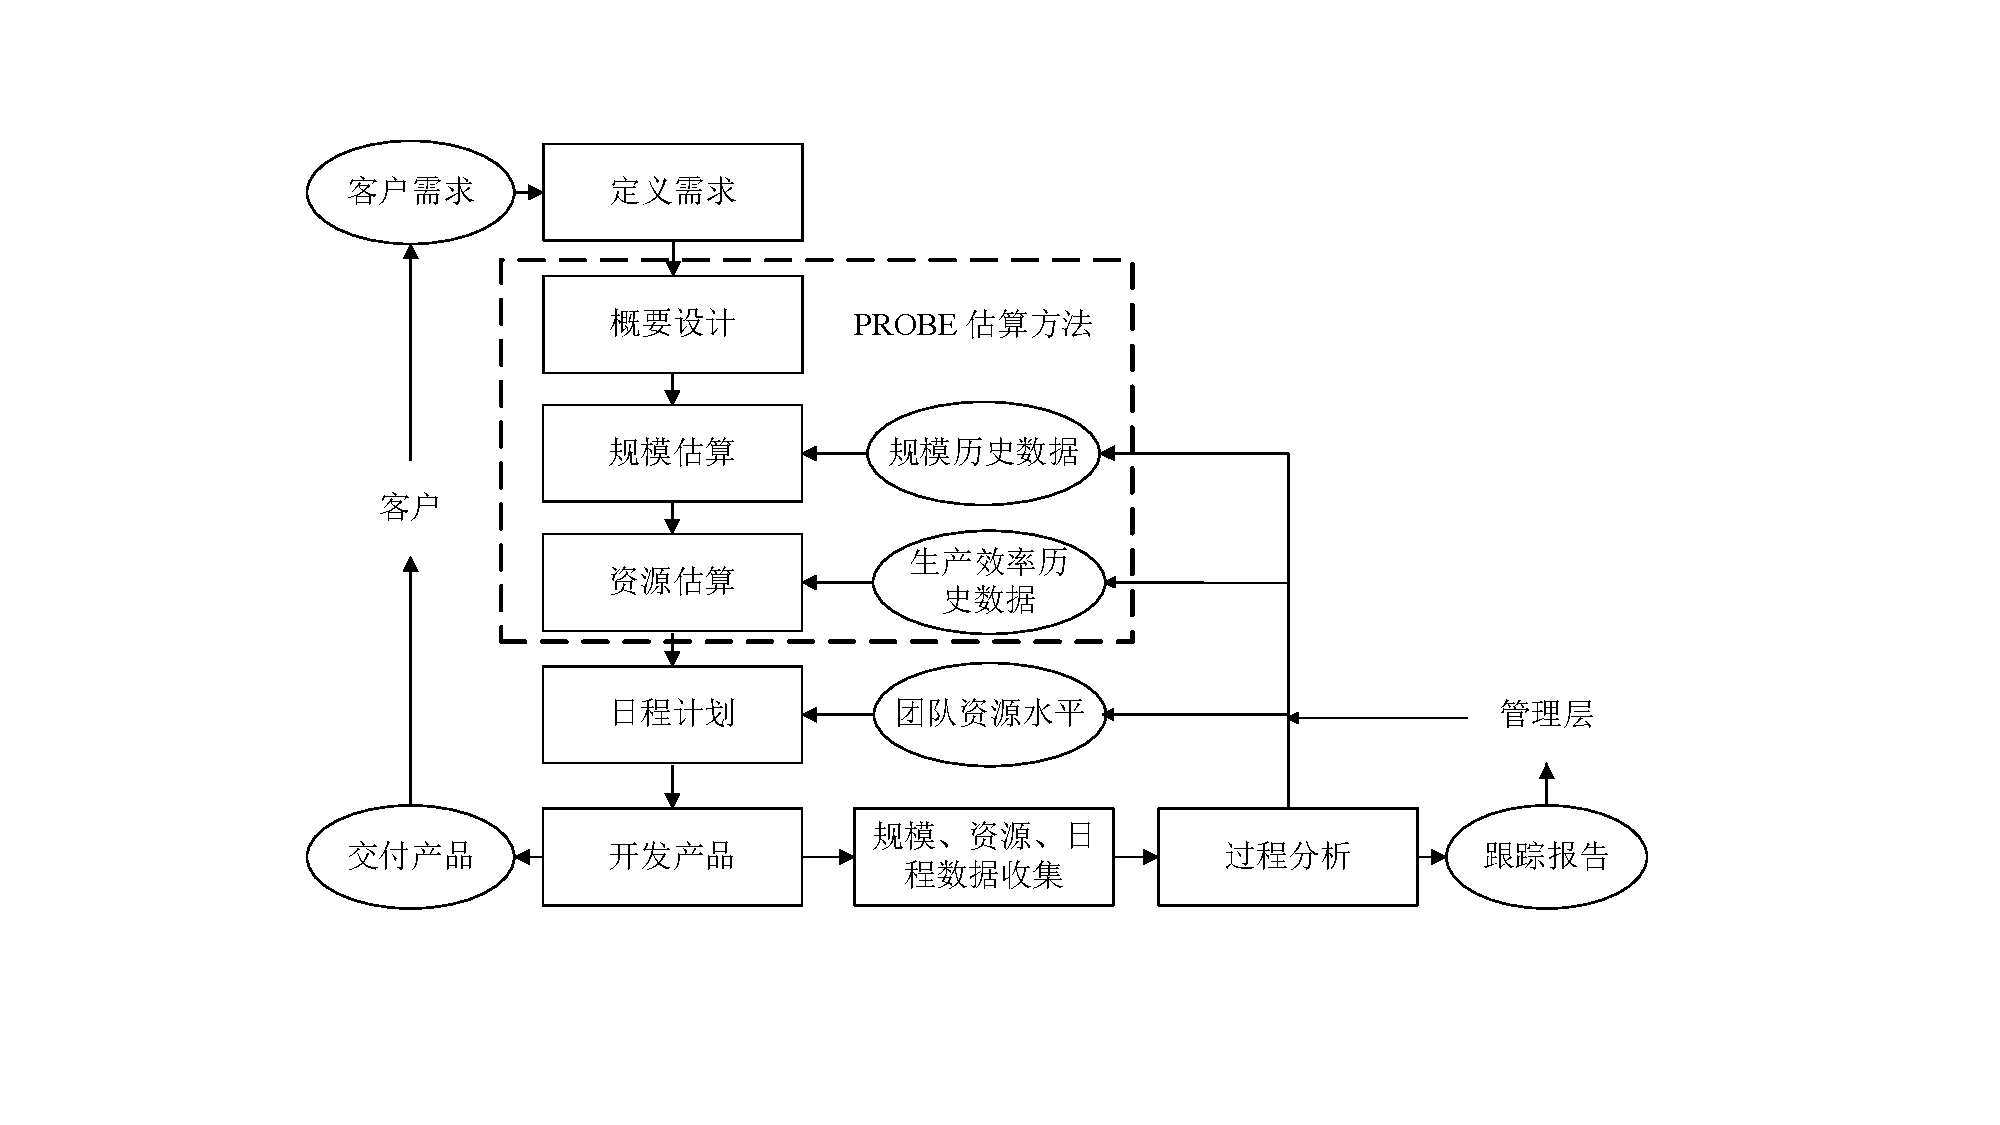
\includegraphics[width=0.5\textwidth]{images/通用计划框架.pdf}
    \vspace{-1em}
\end{figure}
\end{problem}

\begin{problem}
应对风险的典型策略有哪些?请举例说明。
\end{problem}

\begin{problem}
为了确保最终软件产品的质量,在项目计划阶段应该注意哪些问题?
\end{problem}

\subsection{团队项目规划:TSP项目启动}

\subsubsection{TSP的九次会议}
\begin{figure}[H]
    \vspace{-0.5em}
	\centering
	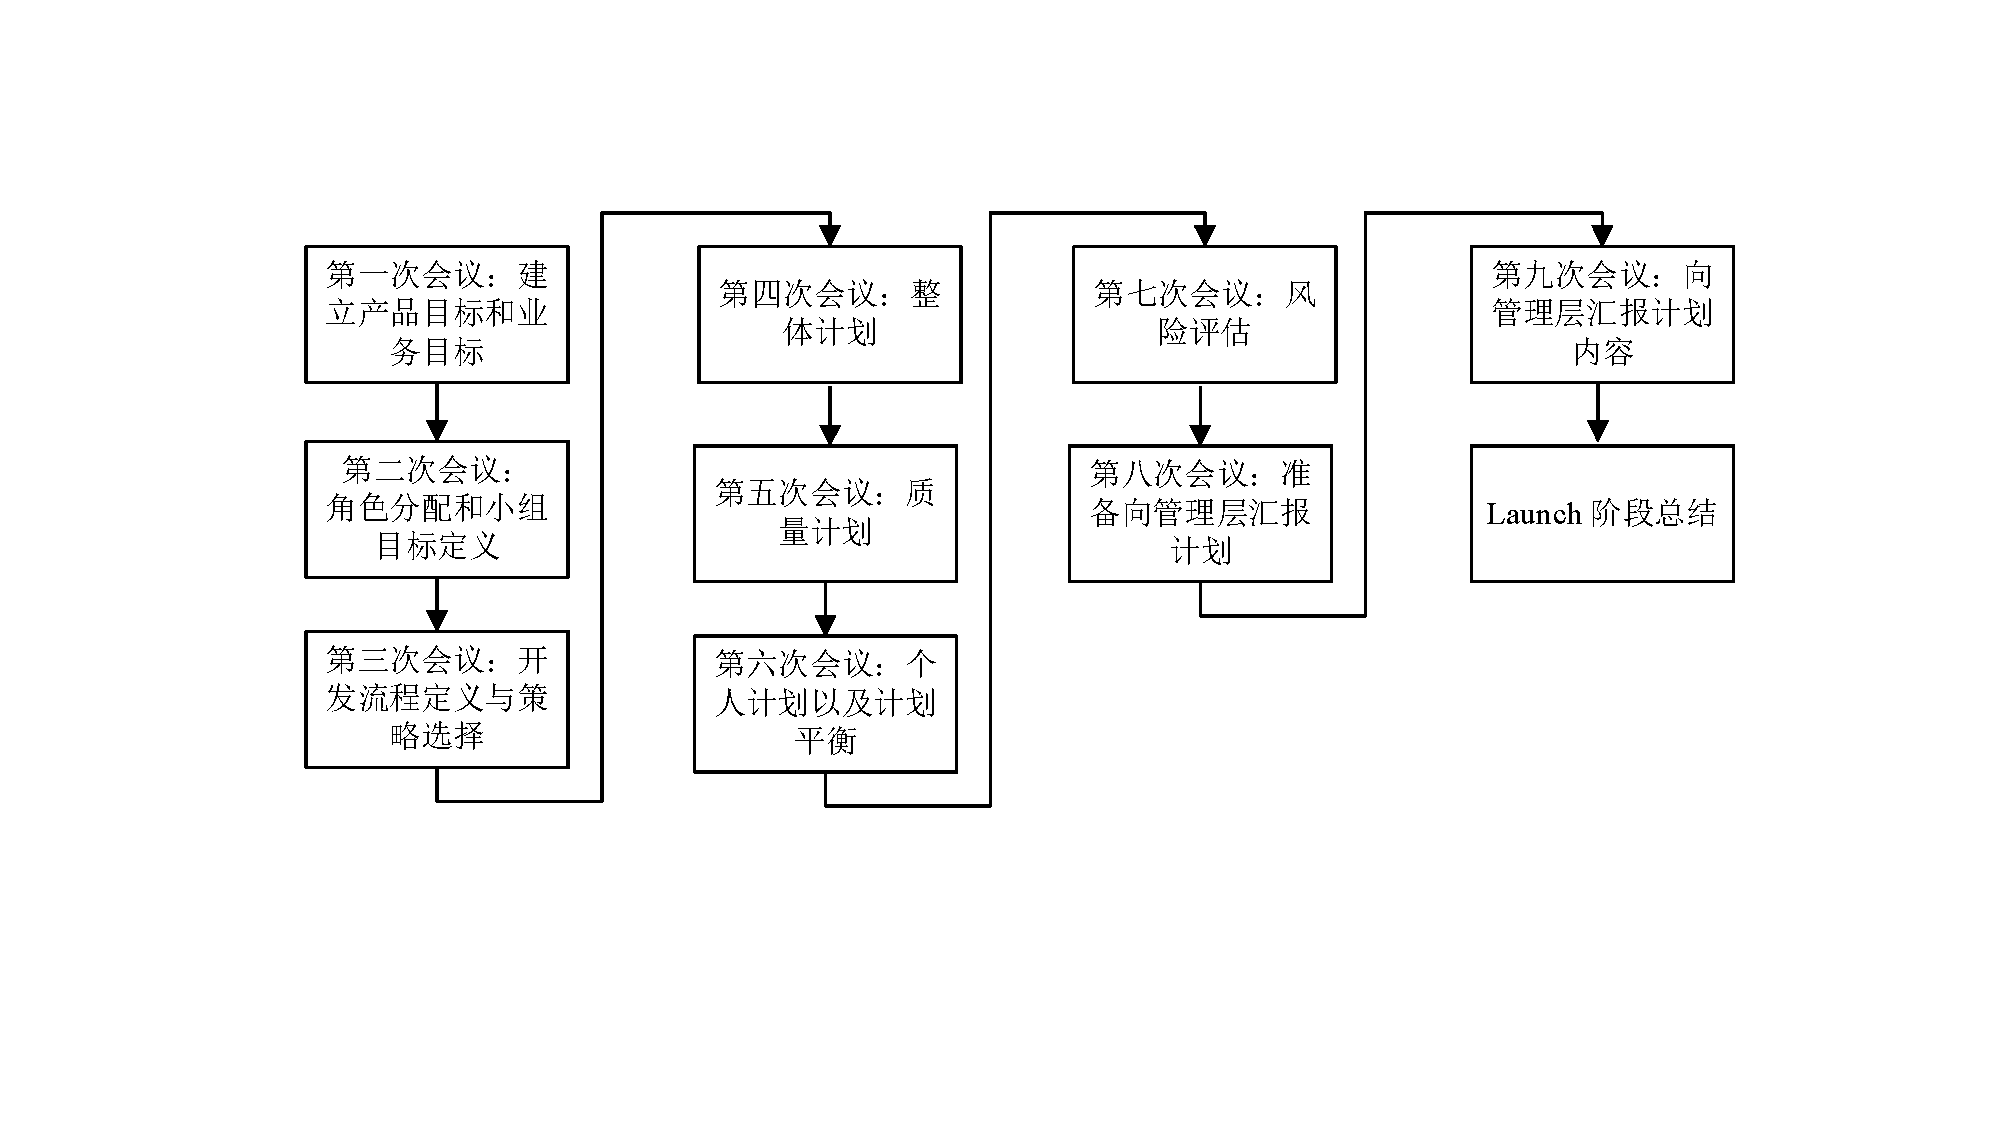
\includegraphics[width=0.85\textwidth]{images/TSP的九次会议.pdf}
    \vspace{-1em}
\end{figure}
几个认识:
\begin{itemize}
    \item 错误的认识:软件开发阶段理解为注入缺陷的阶段,软件测试阶段理解为消除缺陷的阶段
    \item 正确的认识:开发和测试都是既有可能引入缺陷,也有可能消除缺陷的阶段
\end{itemize}

项目完成的实际时间由什么决定?最晚完成的工作的人决定的

经过平衡的计划和没有平衡的计划有什么不一样?更有把握去成功

\subsubsection{考试题目}
\begin{problem}
	在 TSP 的团队组建过程中,确定软件开发策略的是第几次会议?
	\uline{C}    
    \vspace{-0.8em}
    \begin{multicols}{4}
        \begin{enumerate}[label=\Alph*.]
            \item 第一次
            \item 第二次
            \item 第三次
            \item 第四次
        \end{enumerate}
    \end{multicols}
    \vspace{-1em}
\end{problem}

\subsection{团队项目跟踪与分析}
\subsubsection{项目跟踪意义}
在项目进展过程中开展跟踪活动的目的在于了解项目进度,以便在项目实际进展和计划产生严重偏差时,可采取适当的纠正措施
\vspace{-0.8em}
\begin{multicols}{2}
    \begin{itemize}
        \item 项目进度滞后与是否需要参照物,即项目计划
        \item 项目跟踪需要管理偏差而采取的纠偏措施
    \end{itemize}
\end{multicols}
\vspace{-1em}

团队项目的跟踪与管理主要包括进度的跟踪(利用不同跟踪方法,例如挣值管理、里程碑评审)、纠偏活动管理

\subsubsection{项目的挣值管理方法}
\paragraph{什么是EVM}~{} \par
项目的挣值管理方法(EVM, Earned Value Managerment)是用来\textbf{客观度量项目进度}的一种项目管理方法
\vspace{-2.2em}
\begin{multicols}{2}
    \begin{itemize}
        \item 每项任务实现附以一定价值(credit)
        \item 100\%完成该项任务,就获得相应的价值
    \end{itemize}
\end{multicols}
\vspace{-1em}

EVM采用与\textbf{进度计划}、\textbf{成本预算}和\textbf{实际成本}相联系的三个独立的变量,进行项目绩效测量

\paragraph{挣值管理实现}~{} \par
\textbf{简单实现}:仅仅关注进度信息
\begin{itemize}
    \item 实现方式
    \begin{itemize}
        \item 首先需要建立WBS,定义工作范围
        \item 其次为WBS中每一项工作定义一个计划价值(PV, Planned Value)
        \item 最后按照一定的规则将某一数值赋给已经完成的工作或者正在进行的工作,该值成为挣值(EV, Earned Value)
    \end{itemize}
    \item 常用规则
    \begin{itemize}
        \item 0-100原则:只有当某项任务完成时,该任务的PV值将转化成EV值
        \item 50-50原则:只需要开始某项任务,即可以赋原PV值的50\%作为EV值,完成时,再加上另外的50\%
        \item 实际完成的工作所需成本AC不对EV值产生任何影响
    \end{itemize}
\end{itemize}

\textbf{中级实现}
\begin{itemize}
    \item 在简单实现的基础上,加入日程偏差的计算,加入了成本线(AC)
    \item 典型计算方式有
    \vspace{-0.8em}
    \begin{multicols}{2}
        \begin{itemize}
            \item 日程偏差SV = EV $-$ PV
            \item 日程偏差指数SPI = EV/PV;
        \end{itemize}
    \end{multicols}
    \vspace{-1em}
\end{itemize}

\textbf{高级实现}:添加预测线(BAC),当任务足够多的时候,我们就可以让预测线尽可能平直,同时我们延伸挣值(EV),找到与预测线(BAC)的交点,我们就可以明确项目的落后时间

\paragraph{挣值管理图解}~{} \par
\begin{figure}[H]
    \vspace{-0.5em}
	\centering
	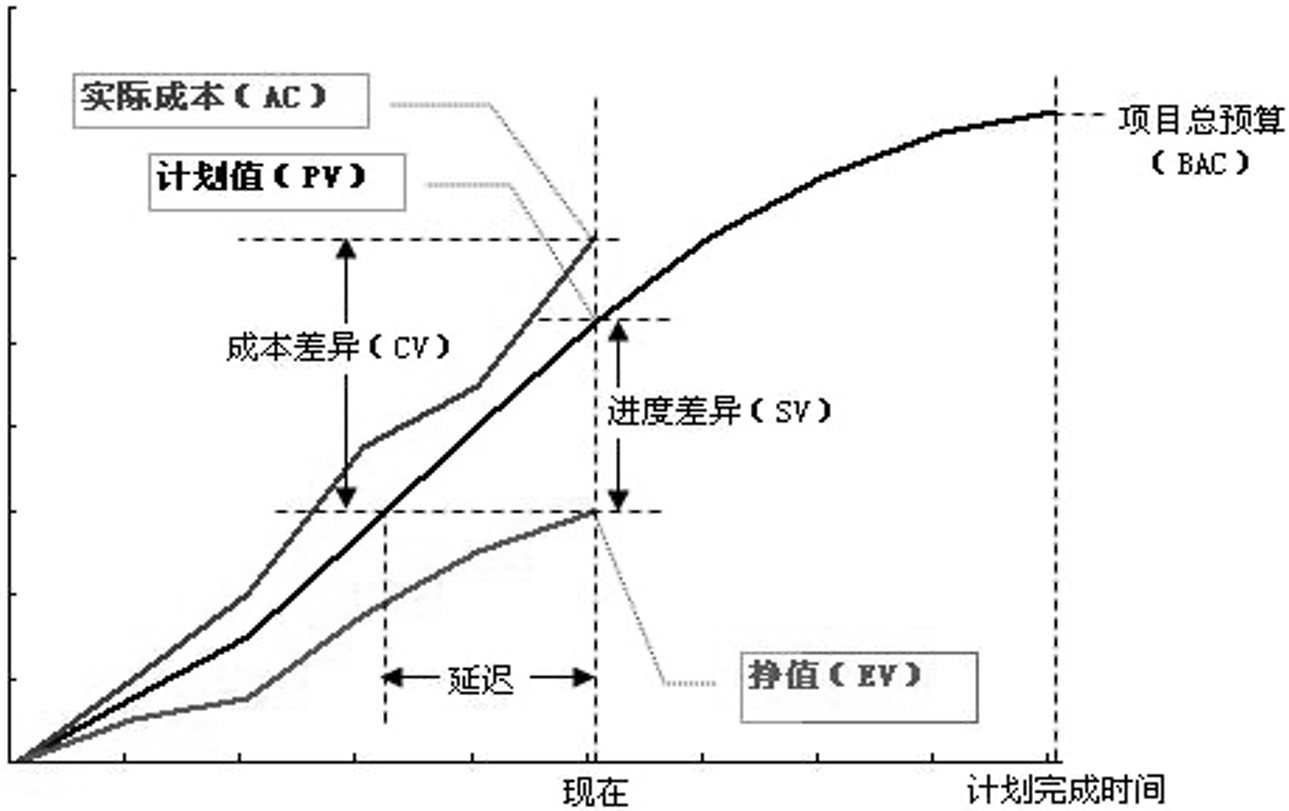
\includegraphics[width=0.6\textwidth]{images/挣值管理图解.png}
    \vspace{-1em}
\end{figure}

\begin{itemize}
    \item 上面的线是为了获取这些挣值付出的实际代价,这个线和挣值之间的差异是成本差异
    \item 中间的线是预算(每天需要完成多少挣值)BAC,理想情况下是一条直线
    \item 下面的线是挣值(实际的进展情况)EV,和owner value有关,对应plan value
    \item 实际获取挣值和预计获取挣值的差异是进度差异
    \item 挣值管理会带来什么好处?可以很好的适应项目的动态变化
\end{itemize}

\paragraph{挣值管理的度量}~{} \par
\begin{itemize}
    \item BAC表示按照PV值的曲线,当项目完成的时候所需预算或者时间
    \item 成本差异CV = EV $-$ AC,表示的是已经完成的工作与所消耗的成本的差异。可以表示为消耗的时间,也可以表示为消耗的资金
    \item 成本差异指数CPI = EV/AC,表示单位成本创造的价值
    \begin{itemize}
        \item CPI < 1说明成本超支;CPI = 1说明成本与预期一致;CPI > 1说明成本低于预期
    \end{itemize}
    \item 日程偏差SV = EV $–$ PV,表示进度偏差
    \begin{itemize}
        \item SV < 0表示进度落后;SV = 0表示进度正常;SV > 0表示进度超前
    \end{itemize}
    \item 日程偏差指数SPI = EV/PV
    \item 预计完成成本EAC = AC + (BAC $-$ EV)/CPI = BAC/CPI,表示的是按照目前的进展已经成本消耗情况,整个项目完成的时候所需消耗的成本
\end{itemize}

\paragraph{挣值管理的应用}~{} \par
发现项目已经滞后
\vspace{-0.8em}
\begin{multicols}{2}
    \begin{itemize}
        \item 削减功能,使得已经完成的任务的EV值增加
        \item 通过加班或加人等手段,提升获取EV值速度
    \end{itemize}
\end{multicols}
\vspace{-1em}

\textbf{例:}EV值显示的项目落后可能是假象,在实际项目过程中,可以采用周报数据的形式来跟踪 EV 值

\begin{wraptable}{r}{0.5\textwidth}
    \centering
    \vspace{-1em}
    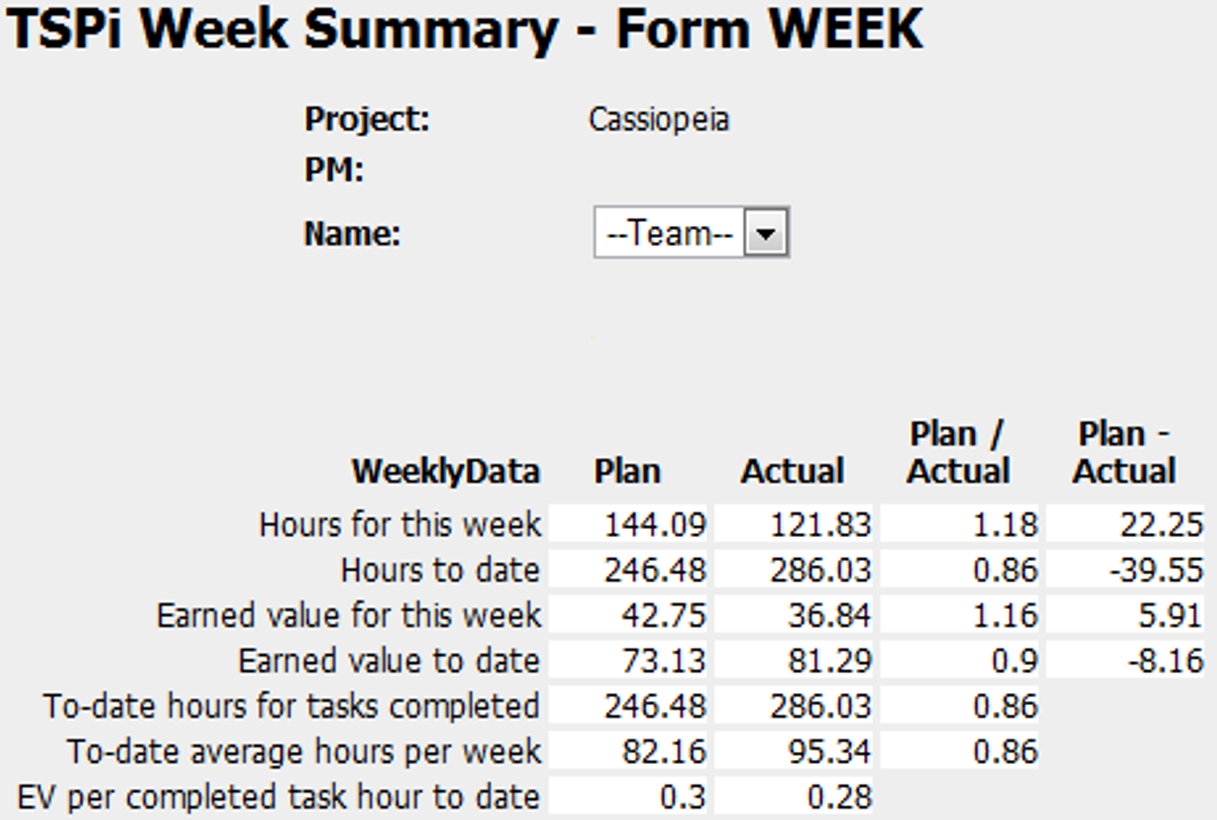
\includegraphics[width=0.5\textwidth]{images/EVM应用示例.png}
    \vspace{-3.5em}
\end{wraptable}
基于图表事实,基本可以得出如下结论:
\begin{itemize}
    \item 项目小组的工作略有提前
    \item 从整体看,项目小组的估算略有偏差,低估了工作难度
    \item 之所以项目目前进度仍然超前,是由于整个团队投人了比预计更多的资源
    \item 按照项目目前的进展情况,整个团队不需要调整,甚至可以相对于以前数周的工作负荷适当减轻负荷
\end{itemize}

\paragraph{挣值管理的局限性}~{} \par
\begin{itemize}
    \item 一般不能应用软件项目的质量管理
    \item 需要定量化的管理机制,这就使得在一些探索型项目以及常用的敏捷开发方法中的应用受到限制
    \item 完全依赖项目的准确估算,然而在项目早期,很难对项目进行非常准确的估算
\end{itemize}

\paragraph{另一种挣值管理变形:燃尽图}~{} \par
\begin{figure}[H]
    \vspace{-0.5em}
	\centering
	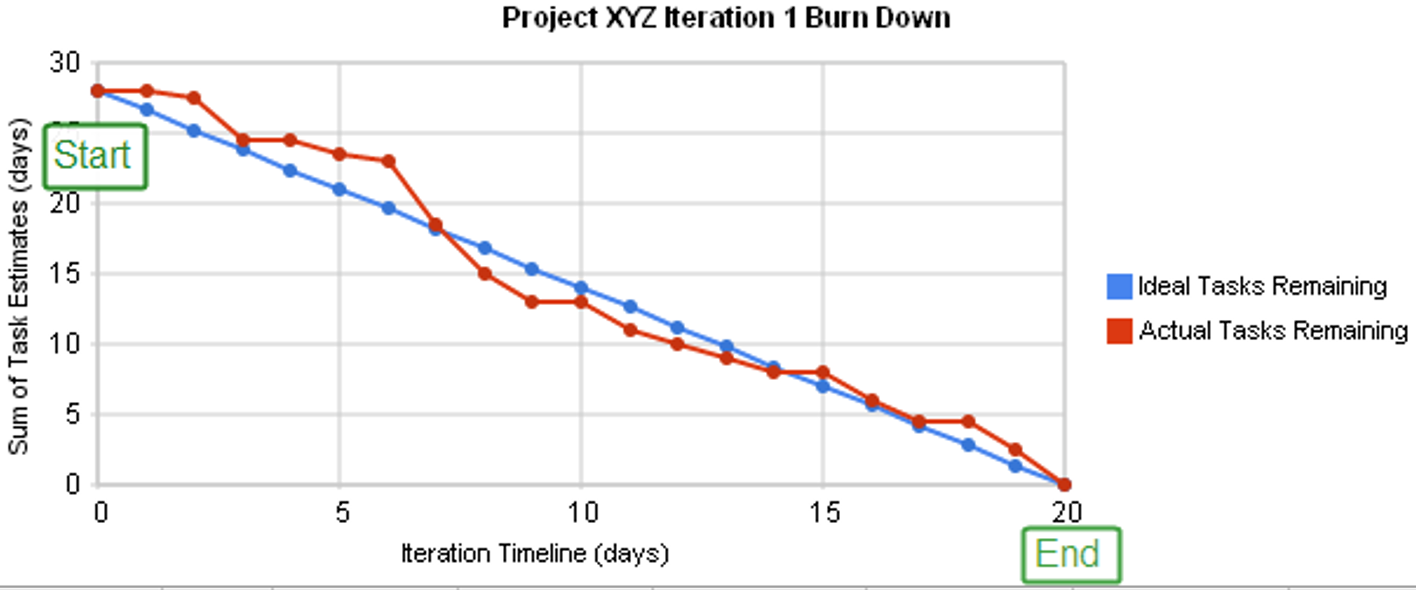
\includegraphics[width=0.63\textwidth]{images/燃尽图}
    \vspace{-1em}
\end{figure}
燃尽图是简单的挣值管理的变形,是剩下的工作占的百分比

\paragraph{考试题目}~{} \par
\begin{problem}
	下列关于挣值管理方法的描述中错误的是?
	\uline{C}    
    \vspace{-0.8em}
    \begin{multicols}{2}
        \begin{enumerate}[label=\Alph*.]
            \item 这是一种可以用来跟踪项目预算消耗的方法
            \item 这种方法高度依赖估算准确性
            \item 这种方法可以支持质量管理
            \item 这种方法可以用来跟踪项目进度
        \end{enumerate}
    \end{multicols}
    \vspace{-1em}
\end{problem}

\subsubsection{里程碑评审}
软件项目的里程碑往往是指某个时间点,用以标记某些工作的完成或者阶段的结束。典型的里程碑事件:
\vspace{-0.8em}
\begin{multicols}{4}
    \begin{itemize}
        \item 完成某项工作
        \item 获干系人签字认可
        \item 完成某产物的评审
        \item 修改或交付某产物
    \end{itemize}
\end{multicols}
\vspace{-1em}

里程碑评审的审查内容包括:
\vspace{-0.8em}
\begin{multicols}{2}
    \begin{itemize}
        \item 项目相关的承诺,如日期、规格、质量等等
        \item 项目各项计划的执行状况
        \item 项目当前的状态讨论
        \item 项目面临的风险讨论等
    \end{itemize}
\end{multicols}
\vspace{-1em}

里程碑评审也可用于质量管理

\subsubsection{其他类型跟踪方法}
\vspace{-0.8em}
\begin{multicols}{3}
    \begin{itemize}
        \item 日程计划跟踪
        \item 承诺计划跟踪
        \item 风险计划跟踪
        \item 数据收集计划跟踪
        \item 沟通计划跟踪
    \end{itemize}
\end{multicols}
\vspace{-1em}

\subsubsection{纠偏活动的管理}
典型的纠偏活动包括:偏差原因分析、纠偏措施定义、纠偏措施管理
\begin{itemize}
    \item 偏差原因分析:收集偏差相关的各种信息,基于收集到的信息,开展充分的分析工作,找出偏差的根本原因
    \item 纠偏措施定义:确认偏差的根本原因,就可以有针对性地定义纠偏的措施
    \item 纠偏措施管理:管理纠偏措施直到结项
\end{itemize}

\subsubsection{项目审查}
审查的内容包括:
\vspace{-0.8em}
\begin{multicols}{3}
    \begin{enumerate}[label=\arabic*.]
        \item 项目相关的承诺,如日期、规格、质量等等
        \item 项目各项计划的执行状况
        \item 项目当前的状态讨论
        \item 项目面临的风险讨论
        \item 其他计划跟踪
        \item 日程计划跟踪
        \item 承诺计划跟踪
        \item 风险计划跟踪
        \item 数据收集计划跟踪
        \item 沟通计划跟踪
    \end{enumerate}
\end{multicols}
\vspace{-1em}

\subsection{项目总结}
\subsubsection{项目总结的定义}
\begin{itemize}
    \item 项目总结需要系统化有条理的进行,才能不遗漏重要的内容
    \item 因此往往需要事先定义总结过程,然后就按部就班地开展总结工作
\end{itemize}

\subsubsection{一般项目总结流程}
基于PMBOK的总结方式,包含范围管理、时间管理、成本管理、质量管理、人力资源管理、沟通管理、风险管理、采购管理和整合管理9大知识领域
\begin{enumerate}[label=\arabic*.]
    \item 项目范围包括产品范围和项目范围。对项目范围管理的总结应当主要关注项目的需求开发过程与变更管理中的得失,对需求管理实际执行情况的差距进行原因分析,找到改进的机会
    \item 时间管理所关注的就是项目的日程计划以及对日程计划的跟踪和管理状况。因此主要考察计划的准确程度以及各个里程碑的偏差情况
    \item 成本管理包括对成本进行估算、预算和控制的各个过程,从而确保项目在批准的预算内完工
    \item 质量管理包括执行组织确定质量政策、目标与职责的各过程和活动,从而使项目满足其预定的需求
    \item 人力资源管理包括组织、管理与领导项目团队的各个过程
    \item 沟通管理包括为确保项目信息及时且恰当地生成、收集、发布、存储、调用最终处置所需的各个过程
    \item 风险管理包括风险管理规划、风险识别、风险分析、风险应对规划和风险监控等各个过程
    \item 采购管理包括从项目组织外部采购或获得所需产品、服务或成果的各个过程
    \item 整合管理包括为识别、定义、组合、统一与协调项目管理过程组的各过程及项目管理活动而进行的各种过程和活动
\end{enumerate}

\subsubsection{TSP项目总结方式}
\begin{enumerate}[label=\arabic*.]
    \item 准备阶段
    \item 过程数据评审阶段:该阶段往往由过程经理或者质量经理带领整个团队分析过程数据,识别过程改进机会
    \begin{itemize}
        \item 可以结合典型TSP团队角色,逐个讨论改进领域。如团队领导力、计划准确性、过程优劣、质量管理能力、开发环境以及配置管理等。
        \item 此外,也可以就TSP教练的作用进行评价。
        \item 过程数据评审阶段还要求开发团队的所有成员都整理过程改进提案(PIP):PIP是TSP过程中供开发人员在日程工作中记录改进想法的工具。其基本思想是积累小的改进,慢慢形成大的改进。在软件开发过程中,重大的改进机会不多,因此,往往需要从小做起,慢慢积累之后,就会形成对原有过程的显著改进。小的改进机会虽然多,但是容易被遗忘,PIP的作用就在于提供了一个标准表格工具,允许软件工程师时时记录改进方案。在项目总结阶段,将开发过程中记录的所有PIP整理出来,形成整个开发周期的过程改进提案,供讨论,以确定下个开发周期要实施的过程改进。
    \end{itemize}
    \item 人员角色评价阶段(角色包括项目组长、计划经理、开发经理、质量经理、过程经理和支持经理)
    \item 总结报告撰写阶段
\end{enumerate}

\subsubsection{通用项目总结流程}
\vspace{-0.8em}
\begin{multicols}{3}
    \begin{enumerate}[label=\arabic*.]
        \item 准备阶段
        \item 总结阶段
        \item 报告阶段
    \end{enumerate}
\end{multicols}
\vspace{-1em}

\subsubsection{项目总结的意义}
提供一个系统化的方式来总结经验教训、防止犯同样的错误、评估项目团队绩效、积累过程数据等,给项目团队成员持续学习和改进的机会

\subsection{项目管理支持活动}
项目管理支持活动包含:配置管理、度量和分析、决策分析和根因分析

\subsubsection{配置管理}
\paragraph{配置管理的目的}~{} \par
建立与维护工作产品的完整性

\paragraph{配置管理的概念}~{} \par
配置项:
\begin{itemize}
    \item 在配置管理当中作为单独实体进行管理和控制的工作产品集合
    \item 典型的可能作为配置项纳入配置管理的工作产品包含过程说明文档、项目开发计划文档、需求规格说明书、设计规格说明书、设计图表、产品规格说明书、程序代码、开发环境,如特定版本的编译器等、产品数据文件、产品技术文件、用户支持文档
\end{itemize}

基线:基线是一个或多个配置项及相关的标识符的代表,是一组经正式审查同意的规格或工作产品集合,是未来开发工作或交付的基础,而且只能经由严格的变更控制程序才能改变
\begin{itemize}
    \item 发布一个基线包括该基线所有的配置项以及这些配置项的最新变更,因此,可以将基线作为接下来工作的基础
    \item 典型的发布基线时间点为需求分析之后、设计完成之后、单元测试之后以及最终产品发布
    \item 是配置项持续演进的稳定基础
\end{itemize}

\paragraph{配置管理的流程}~{} \par
配置管理是用管理的手段监督和指导如下工作的流程[CMMI 2006]
\vspace{-0.8em}
\begin{multicols}{2}
    \begin{enumerate}[label=\arabic*.]
        \item 识别和记录配置项的物理特性和功能特性
        \item  控制上述特性的变更
        \item 记录和报告变更过程和相应的配置项状态
        \item 验证配置项是否与需求一致
    \end{enumerate}
\end{multicols}
\vspace{-1em}

\begin{wraptable}{r}{0.65\textwidth}
    \centering
    \vspace{-1.5em}
    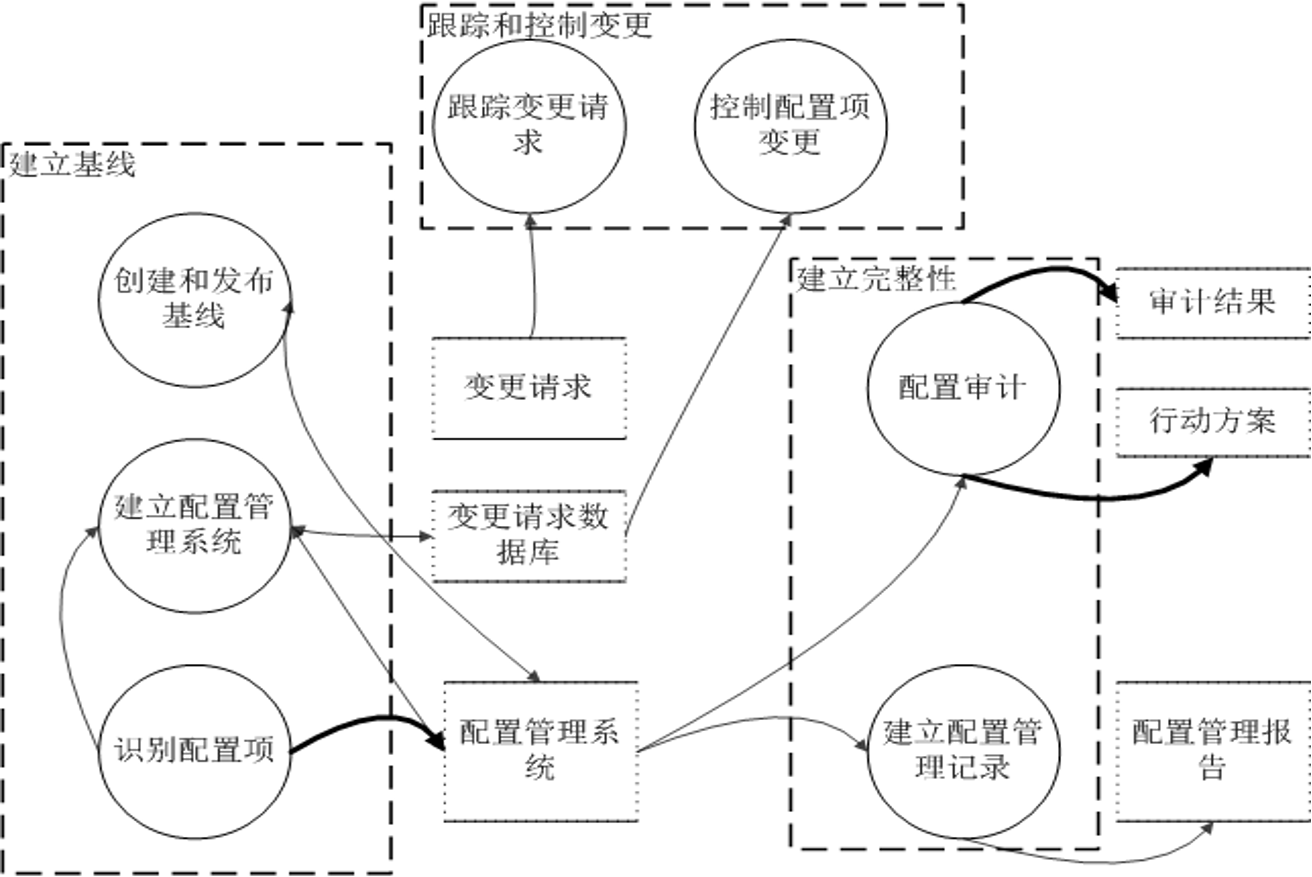
\includegraphics[width=0.55\textwidth]{images/配置管理活动.png}
    \vspace{-5.5em}
\end{wraptable}
\paragraph{配置管理活动}~{} \par
\begin{enumerate}[label=\arabic*.]
    \item 识别配置项
    \item 建立配置管理系统
    \item 创建和发布基线
    \item 跟踪变更请求
    \item 控制配置项变更
    \item 建立配置管理记录
    \item 配置审计
\end{enumerate}

\paragraph{考试题目}~{} \par
\begin{problem}
请解释配置管理中配置项和产品基线的概念,并设计一个流程对单元测试后已经纳入配置库的代码,修改集成测试中的若干问题后,该如何控制变更。

配置项和产品基线的概念如上

如何控制变更:
\begin{itemize}
    \item 跟踪变更请求
    \begin{itemize}
        \item 启动变更请求处理程序,将变更情况保存在变更请求数据库中
        \item 分析变更建议和所需进行的修改将对工作产品、进度、日程等造成的影响
        \item 如果变更请求影响到其他基线,则与相关的干系人一起审查这些变更请求,并取得他们的同意
        \item 跟踪变更申请直到结项
    \end{itemize}
    \item 控制配置项变更
    \vspace{-0.8em}
    \begin{multicols}{2}
        \begin{itemize}
            \item 确认这些修订已得授权
            \item 更新配置项
            \item 将旧基线归档保存,并获取新基线
            \item 执行审查,确保该变更没有对基线造成意料外的影响
            \item 上当记录配置项的变更内容和变更理由
        \end{itemize}
    \end{multicols}
    \vspace{-1em}
\end{itemize}
\end{problem}

\subsubsection{度量和分析}
\paragraph{度量和分析简介}~{} \par
意义:在软件项目管理决策的过程中,基于客观的数据很重要,这种客观决策可以显著消除错误决策的风险。而这些客观数据的获得,必须依照一定的流程以正确的方式获得和使用。度量和分析活动就定义了上述客观数据的获取与使用方式。

目的:建立与维持度量能力,以支持管理的信息需要。

\begin{wraptable}{r}{0.6\textwidth}
    \centering
    \vspace{-2em}
    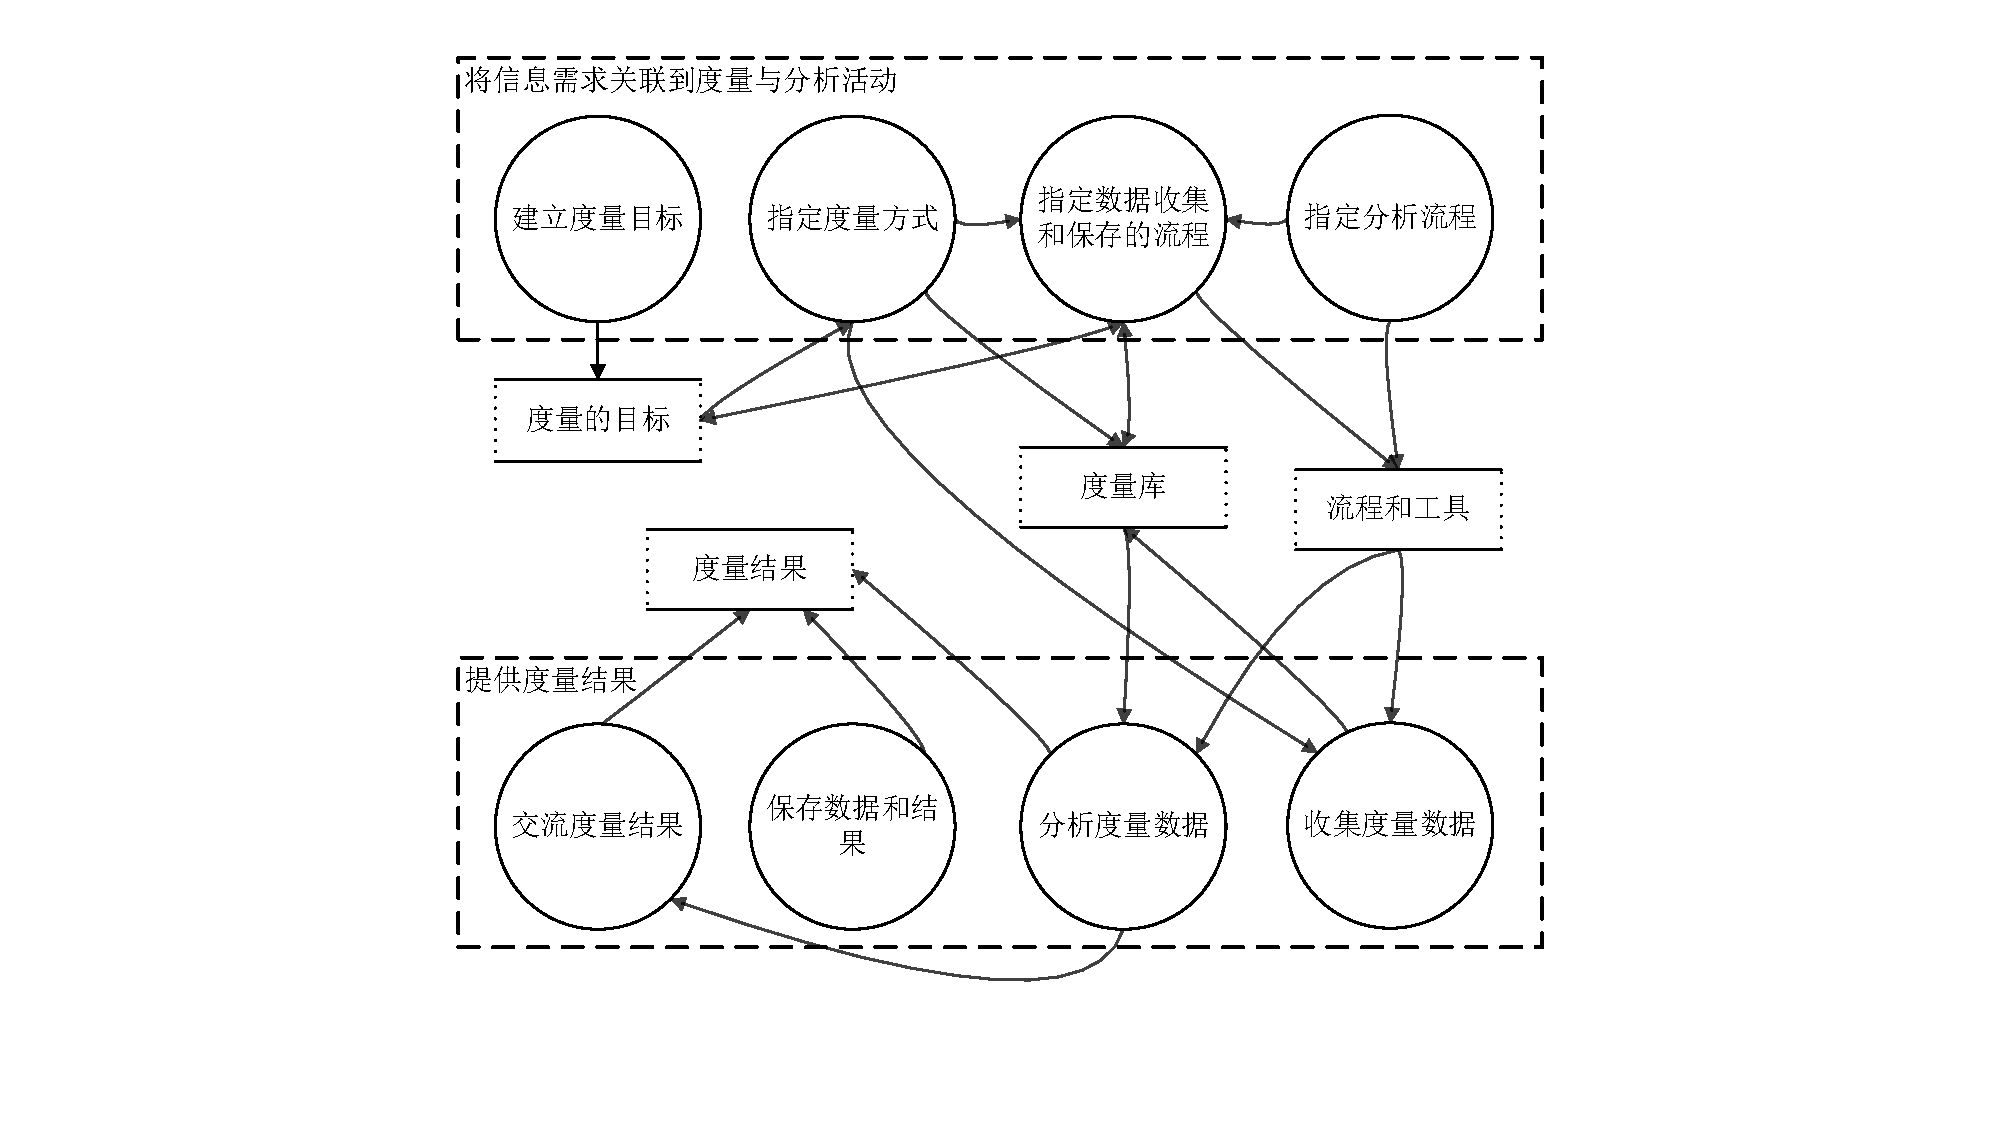
\includegraphics[width=0.6\textwidth]{images/度量与分析活动.pdf}
    \vspace{-7em}
\end{wraptable}
\paragraph{度量和分析活动}~{} \par
\begin{enumerate}[label=\arabic*.]
    \item 建立度量目标
    \item 指定度量方式
    \item 指定数据收集和保存的流程
    \item 指定分析流程
    \item 收集度量数据
    \item 分析度量数据
    \item 保存数据和结果
    \item 交流度量结果
\end{enumerate}

\paragraph{GQM方法的原理和应用}~{} \par
GQM(Goal Question Metric)是一种应用非常广泛的建立软件度量体系的方法,从管理的目标出发,将目标归纳、分解为度量的指标,并把这些指标提炼成可以测量的值,是一种科学的、系统的思考问题的方式
\begin{itemize}
    \item 概念层(目标):目标是为某个特定的对象而定义的。这里的对象是指软件产品、软件过程以及相关的资源等。定义的目标基于不同原因和不同质量模型,也要参考不同的角色视图与特定的环境
    \item 操作层(问题):基于一定的刻画上述目标是否达成或者目标达成的进展情况的模型,使用一系列的问题来定义所研究的对象, 然后得出评价或评估特定目标达成进展情况。所选择的问题应当尽量体现质量相关的话题
    \item 量化层(度量):试图以量化的方式回答上述操作层识别出来的问题
\end{itemize}

\textbf{例:}GQM示例:PM
\vspace{-0.8em}
\begin{multicols}{2}
    \begin{itemize}
        \item G: 确保稳定性、可预测性的开发过程来满足计划的里程碑。
        \item Q: 我的项目是否按照计划的轨迹前进,计划的里程碑都能实现吗?
        \item M: 软件项目开发工作的挥发性(分支、流、变更管理(UCM)活动)。
    \end{itemize}
\end{multicols}
\vspace{-1em}

\textbf{例:}GQM示例:DM
\vspace{-0.8em}
\begin{multicols}{2}
    \begin{itemize}
        \item G: 最大化所有团队贡献者的生产力。
        \item Q: 开发人员能够完成分配给他们的任务吗,或者他们遇到障碍了吗?
        \item M: 由个体或者工作组产生的项目工件的数量
    \end{itemize}
\end{multicols}
\vspace{-1em}

\paragraph{考试题目}~{} \par
\begin{problem}
请结合GQM思想解释PSP过程的基本度量元有哪几个?
\end{problem}

\begin{problem}
描述一下度量和分析活动在一个软件项⽬当中的作用,以及应该如何正确开展?

可以描述度量和分析活动,也可以描述GQM
\end{problem}

\subsubsection{决策分析}
决策分析的意义:错误的决策往往会给项目带来灾难性后果。为了降低这种错误决策的风险,往往需要尽可能基于客观事实和正确的流程来开展决策与分析活动

\begin{wraptable}{r}{0.55\textwidth}
    \centering
    \vspace{-1.5em}
    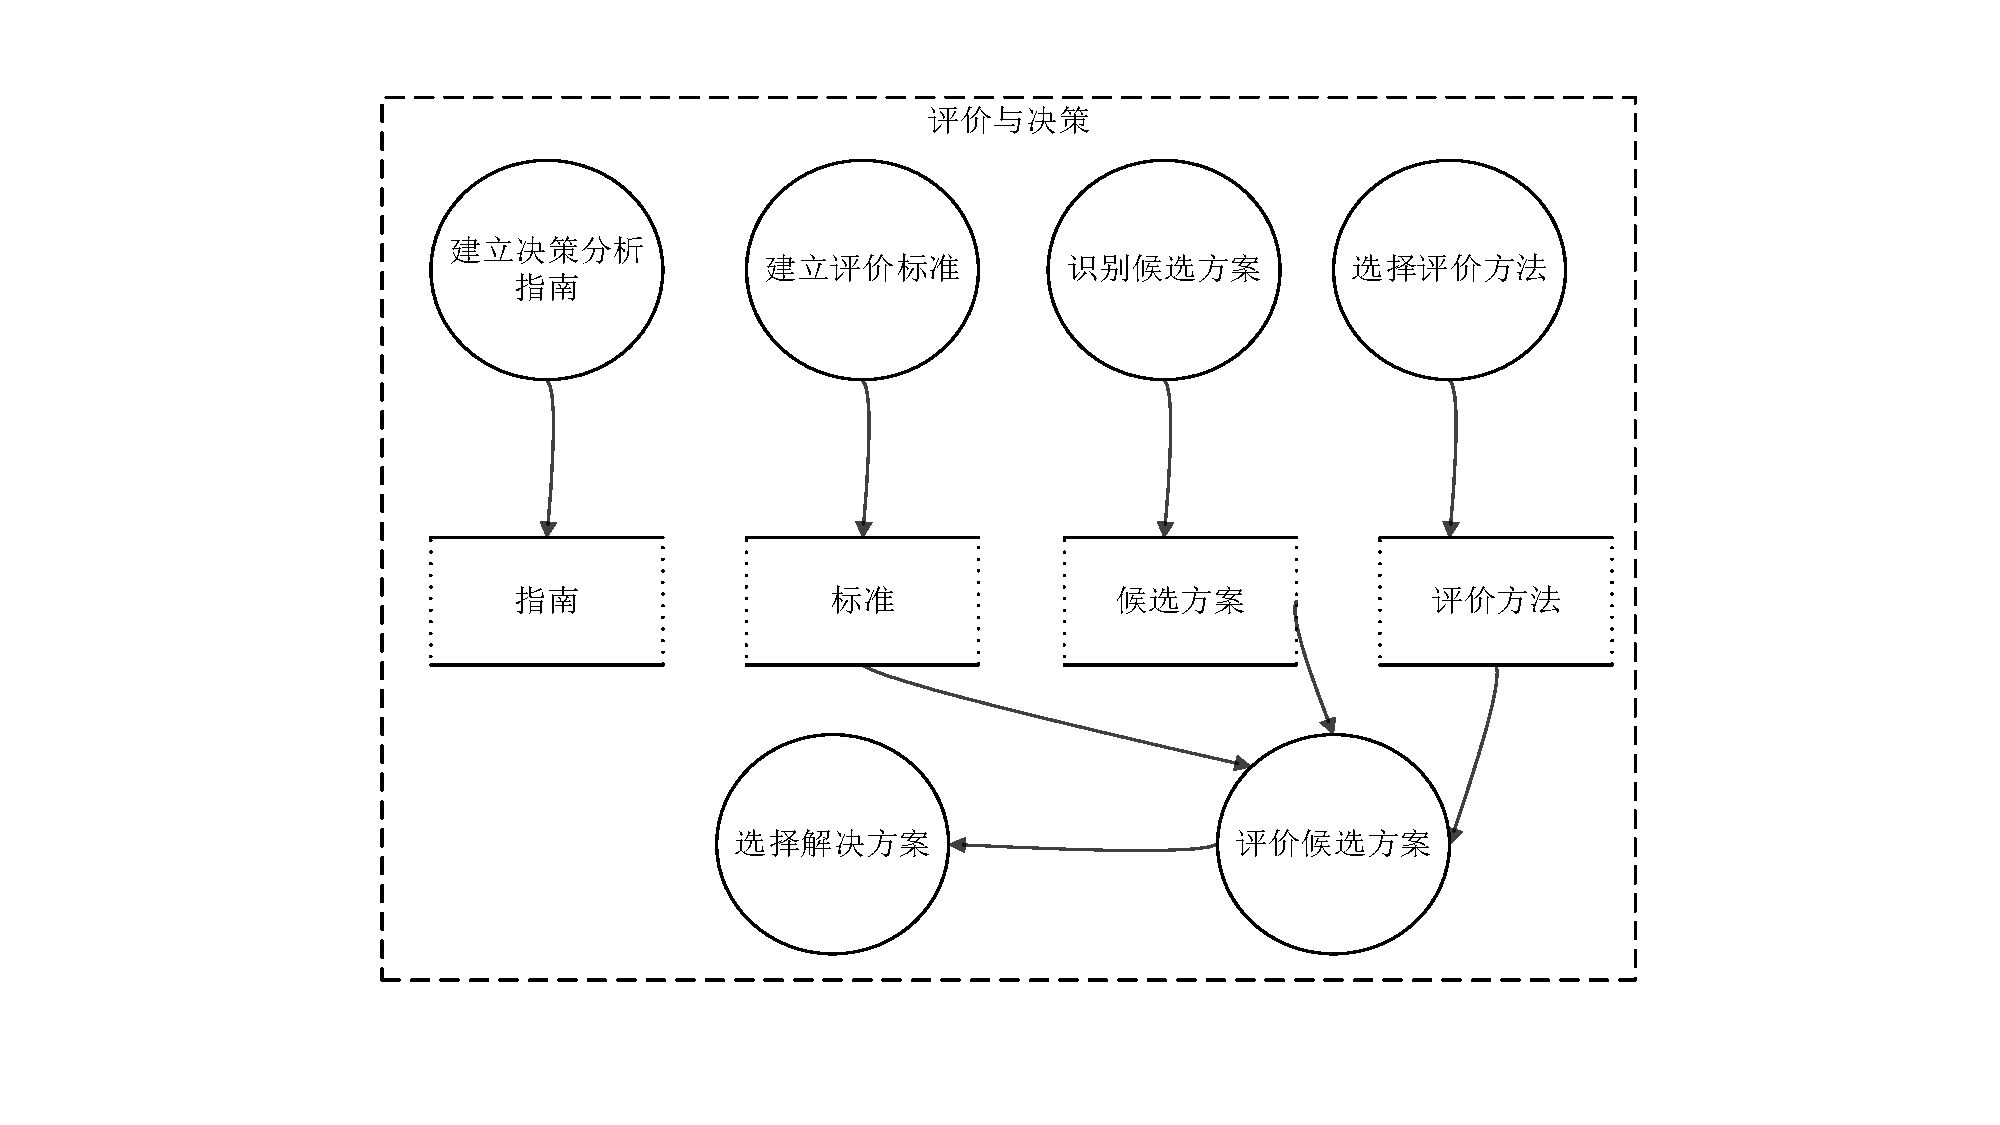
\includegraphics[width=0.55\textwidth]{images/决策分析活动.pdf}
    \vspace{-6.5em}
\end{wraptable}
决策分析往往包含以下活动:
\begin{enumerate}[label=\arabic*.]
    \item 建立决策分析指南
    \item 建立评价标准
    \item 识别候选方案
    \item 选择评价方法
    \item 评价候选方案
    \item 选择解决方案
\end{enumerate}

\subsubsection{根因分析}
避免类似错误反复发生,一个正式根因分析过程往往包含下列的活动:
\vspace{-0.8em}
\begin{multicols}{4}
    \begin{itemize}
        \item 识别和选定问题
        \item 根因分析
        \item 建立改进行动方案
        \item 实施改进,评估效果
    \end{itemize}
\end{multicols}
\vspace{-1em}

\begin{figure}[H]
    \vspace{-0.5em}
	\centering
	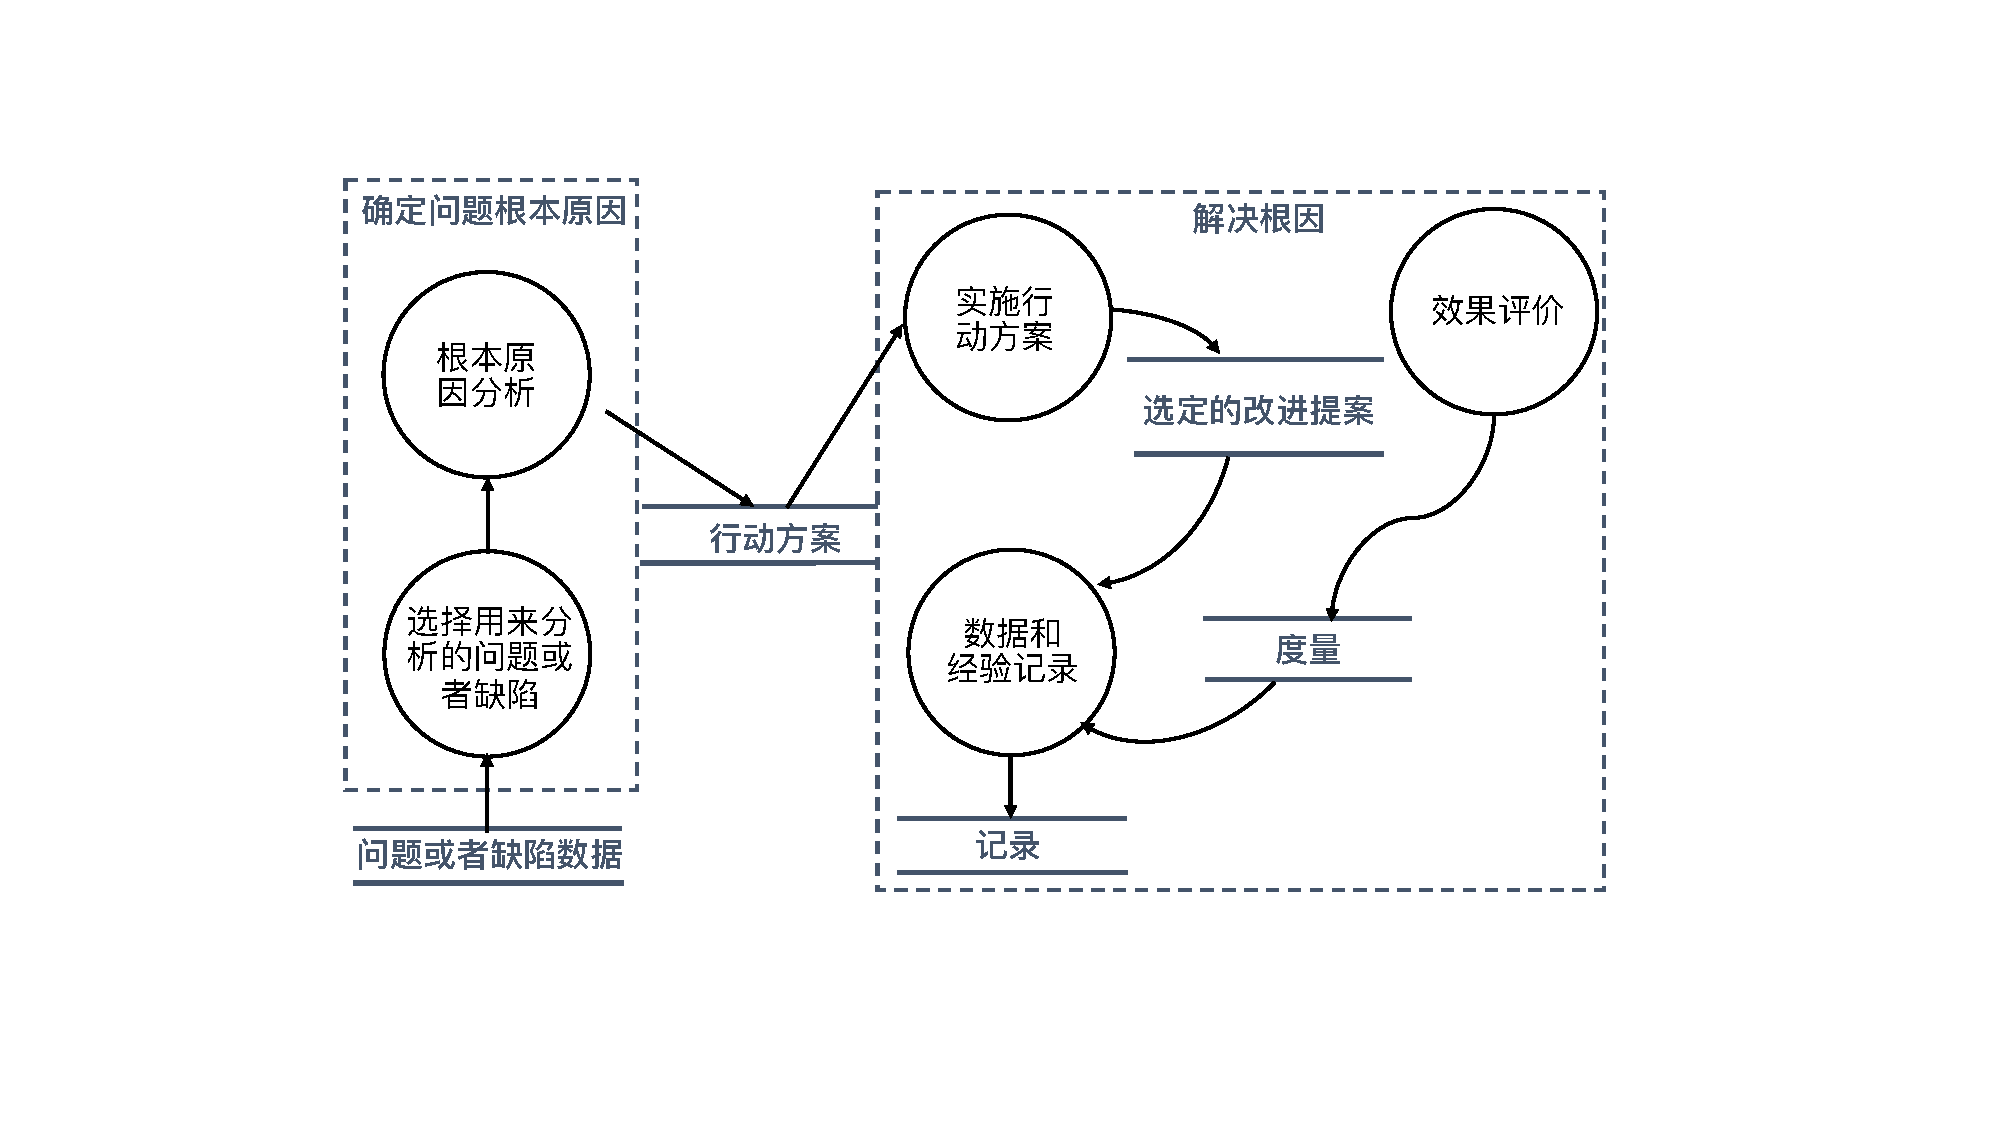
\includegraphics[width=0.63\textwidth]{images/根因分析活动.pdf}
    \vspace{-1em}
\end{figure}
\vspace{-1em}

根因分析典型示例
\begin{figure}[H]
    \vspace{-0.5em}
	\centering
	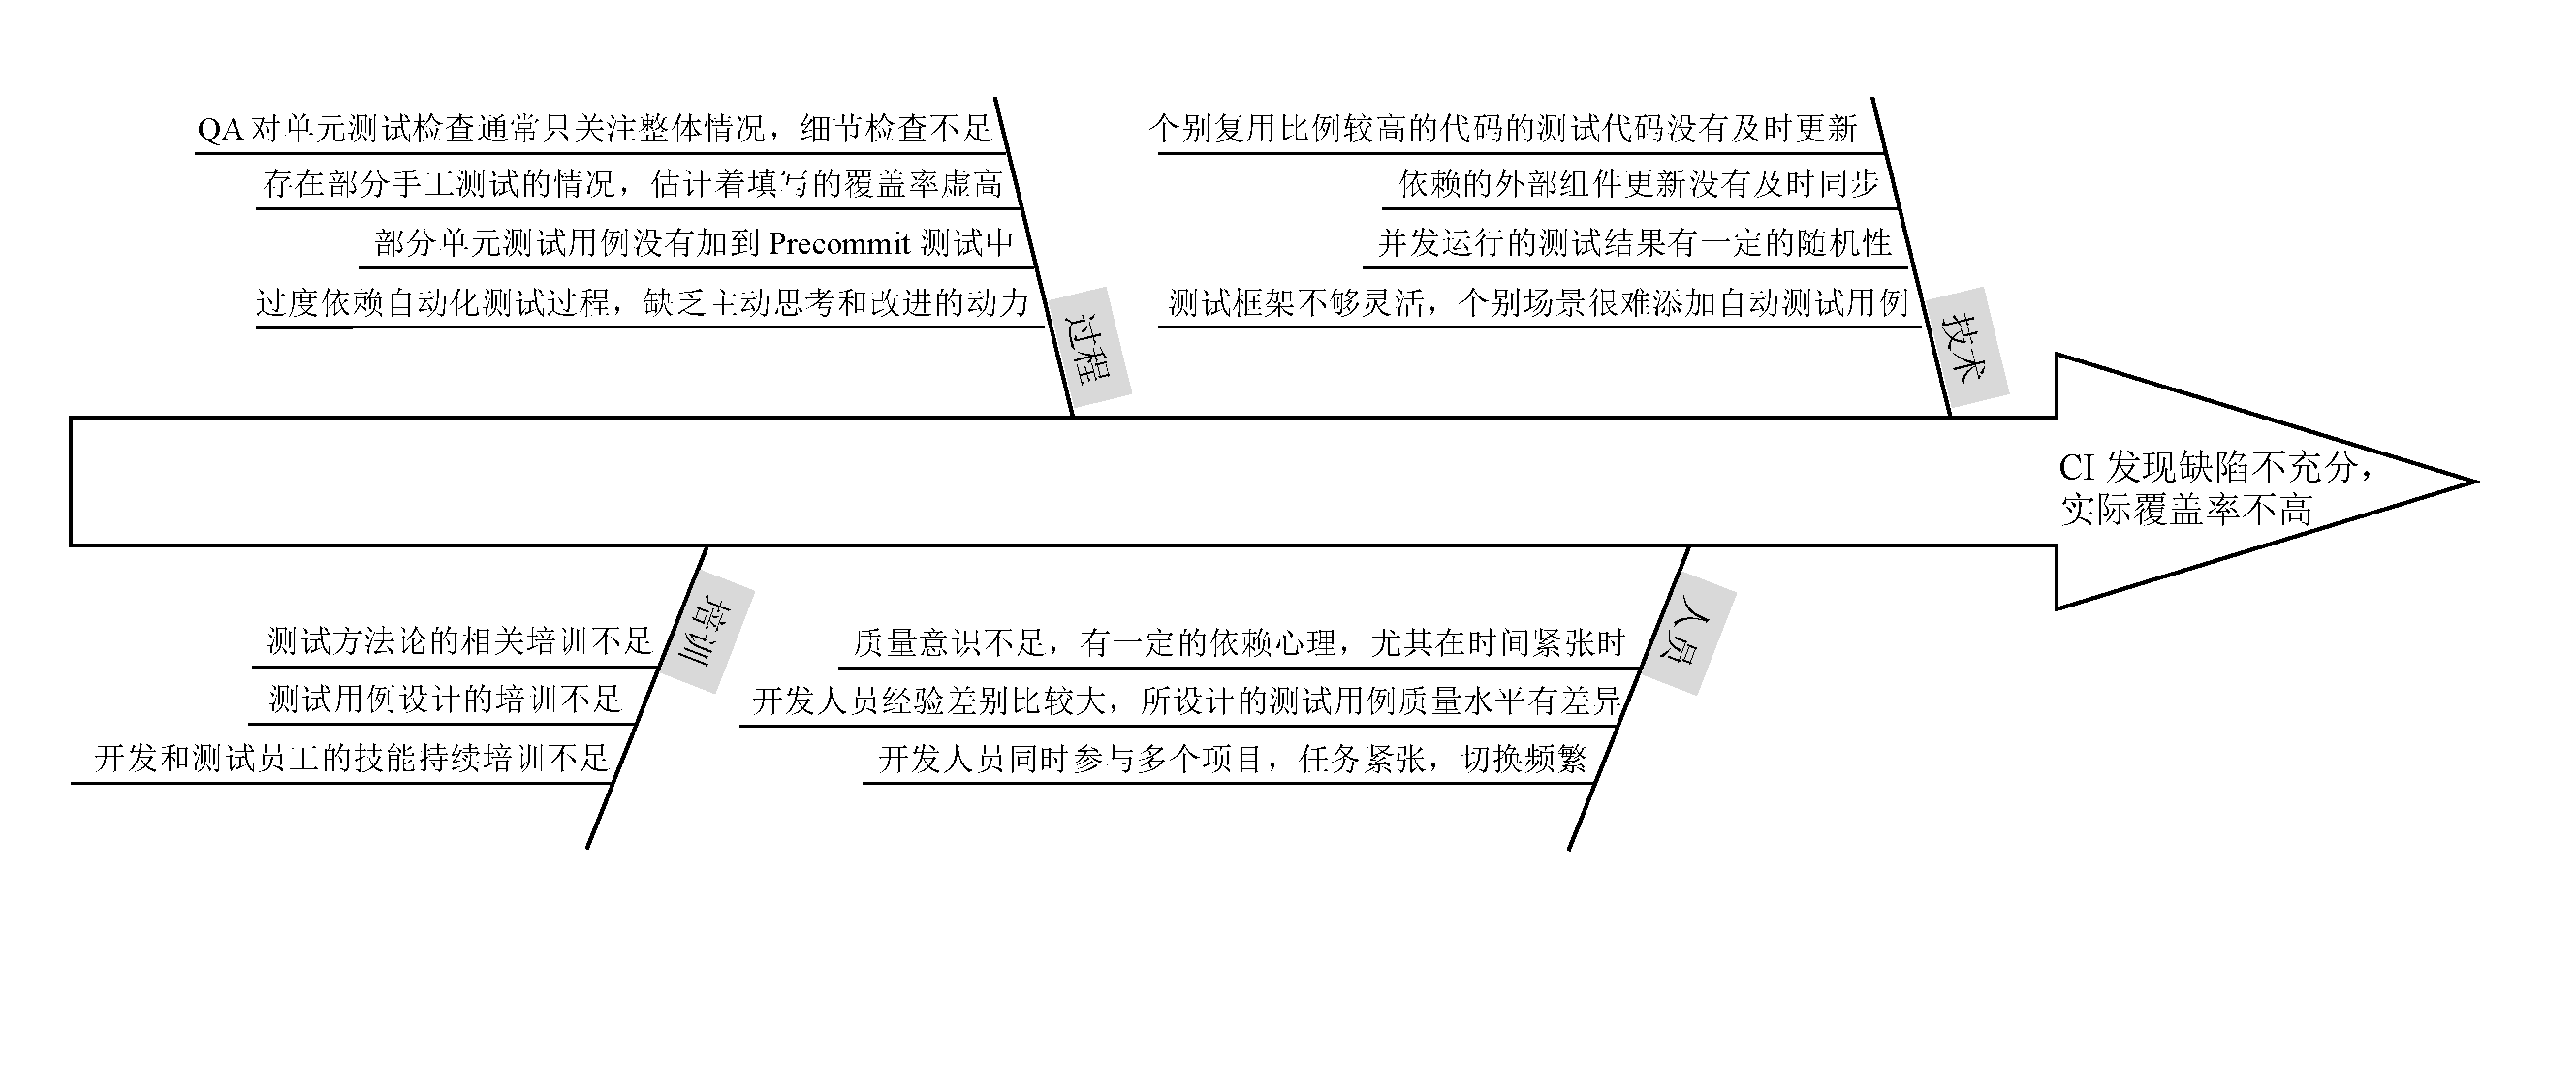
\includegraphics[width=0.9\textwidth]{images/根因分析典型示例.pdf}
    \vspace{-1em}
\end{figure}
\vspace{-1em}

\subsection{团队动力学}
软件开发的特点:
\begin{itemize}
    \item 软件开发是一项\textbf{既复杂又富有创造性}的知识工作
    \item 软件开发:智力劳动,需要处理和讨论极其抽象的概念,并把不同的部分(不可见)整合成一个可以工作的系统
    \begin{itemize}
        \item 要求从事软件开发的工程师
        \begin{itemize}
            \item \textbf{必须全身心地参与工作}:知识工作必须是全身心投入的,任务切换一般需要30分钟才能全身心的投入
            \item \textbf{主观意愿上努力追求卓越}
        \end{itemize}
        \item 要求管理者激励并维持激励:激励手段、维持激励手段
    \end{itemize}
\end{itemize}

管理知识工作的关键规则是:\textbf{管理者无法管理工作者,知识工作者必须实现并学会自我管理}
\begin{itemize}
    \item 要自我管理,知识工作者必须(自我管理的前提条件)
    \vspace{-0.8em}
    \begin{multicols}{3}
        \begin{itemize}
        \item 有积极性
        \item 能做出准确的估算和计划
        \item 懂得协商承诺
        \item 有效跟踪他们的计划
        \item 持续地按计划交付高质量产品
        \end{itemize}
    \end{multicols}
    \vspace{-1em}
    \item 知识工作者实现自我管理:\textbf{胶冻状团队}
\end{itemize}

知识工作者的管理需要的是领导者,而不是经理,领导者需要诚实、有能力、有远见、鼓舞人心

\subsubsection{自主团队}

\paragraph{团队定义}~{} \par
一个团队必须包括至少\textbf{两个成员},他们为了\textbf{共同的目标和愿景}而努力工作,他们每个人都有\textbf{明确的角色}和\textbf{相应的职责定义},任务的完成需要团队成员\textbf{互相依赖和支持}

\paragraph{自主团队的含义}~{} \par
软件工程师所从事的工作一般称之为复杂的知识工作。在这种性质的工作中,实现软件工程师的自我管理往往可以获得最好的工作效率和质量水平。如果整个团队的所有成员都实现了自我管理,也就形成了所谓的自主团队。

\paragraph{自主团队的特点}~{} \par
\vspace{-0.8em}
\begin{multicols}{3}
    \begin{enumerate}[label=\arabic*.]
        \item 自行定义项目的目标
        \item 自行决定团队组成形式以及成员的角色
        \item 自行决定项目的开发策略
        \item 自行决定项目的开发过程
        \item 自行制定项目的开发计划
        \item 自行度量、管理和控制项目工作
    \end{enumerate}
\end{multicols}
\vspace{-1em}

\paragraph{自主团队的必要性}~{} \par
\begin{itemize}
    \item 自主团队可以形成“胶冻态团队”。在这样的团队中存在一种神奇的力量,这种神奇力量弥漫于该团队做的所有工作
    \item 团队成员互相支持,更为重要的是,团队成员在任何时刻都知道应该以怎样的方式帮助别人;团队成员相互信任,有强烈的归属感
    \item 团队在适当的知道会聚集在一起,研究现状,讨论策略
\end{itemize}

\paragraph{自主团队的形成}~{} \par
自主团队不是偶然形成的
\begin{itemize}
    \item 大部分情况下,在团队建立之初,团队成员往往有着不同的目标;缺乏清晰的角色定义和职责安排。对于待开发的产品只有模糊的概念;团队成员也有着不同的工作习惯和工作方法。
    \item 经过一段时间的协同工作,团队成员可以慢慢培养团队协作方式,从而逐渐演化成自主团队
\end{itemize}

\paragraph{自主团队的外部环境}~{} \par
\vspace{-0.8em}
\begin{multicols}{2}
    项目启动阶段获得管理层的支持
    \begin{itemize}
        \item 项目小组应当表现出已经尽最大的可能在满足管理层的需求的工作态度
        \item 项目小组应当在计划中体现定期需要向管理层报告的内容
        \item 项目小组应当向管理层证明他们所制定的工作计划是合理的
        \item 项目小组应当在项目中体现为了追求高质量而开展的工作
        \item 项目小组应当在工作计划中允许必要项目变更
        \item 项目小组应当向管理层寻求必要的帮助
    \end{itemize}
    
    在项目进展过程中获得管理层的支持
    \begin{itemize}
        \item 项目小组应当严格遵循定义好的开发过程开展项目开发过程
        \item 项目小组应当维护和更新项目成员的个人计划和团队计划
        \item 项目小组应当对产品质量进行管理
        \item 项目小组应当跟踪项目进展,并定期向管理层报告
        \item 项目小组应当持续地向管理层展现优异的项目表现
    \end{itemize}
    
\end{multicols}
\vspace{-1em}

\subsubsection{激励方式}
\begin{itemize}
    \item 威逼:完全依靠不同角色的等级关系,通常是上级强制要求下属必须完成某些工作
    \item 利诱:通过许诺一定的好处来吸引下属努力工作
    \item 鼓励承诺:
    \begin{itemize}
        \item 建立承诺文化,利用软件工程师希望得到别人尊重的心理,鼓励他们合理承诺并努力满足承诺,从而得到别人的尊重
        \item 位于马斯洛需求理论的4级以上,应当是主要的方式,并且最好以团队为单位做出承诺
    \end{itemize}
\end{itemize}

\vspace{-0.5em}
\begin{spacing}{1.2}
    \centering
    \begin{longtable}{|m{1.5cm}<{\centering}|m{13.8cm}|}
        \hline
        \textbf{领导方式} & \multicolumn{1}{c|}{\textbf{说明}} \\ \hline
        交易型领导方式 &
        \vspace{-1.1em}
        \begin{enumerate}[label=\arabic*.,leftmargin=1.2em,itemsep=-2pt]
            \item 承诺奖励激励
            \item 人们通常能找到新的方式来获得奖励,同时少做工作
            \item 威逼和利诱属于交易型领导方式
        \vspace{-1.3em}
        \end{enumerate} \\ \hline
        转变型领导方式 &
        \vspace{-1.1em}
        \begin{enumerate}[label=\arabic*.,leftmargin=1.2em,itemsep=-2pt]
            \item 用成就激励
            \item 鼓励承诺属于转变型领导方式
            \item 由于交易型领导方式很少能产生成功并且有创造性的团队,因此\textbf{转变型领导方式是首选}
        \vspace{-2.5em}
        \end{enumerate} \\ \hline
    \end{longtable}
\end{spacing}
\vspace{-5em}


\subsubsection{马斯洛的需求层次理论}
一共有五个层次:生理需求(Physiological)、安全感(Safety)、爱和归属感(social)、获得尊敬(Esteem)、自我实现(Self-Actualization)
\vspace{-0.8em}
\begin{multicols}{2}
    \begin{itemize}
        \item 自我实现是最高的层次
        \item 激励来自为没有满足的需求而努力奋斗
        \item 低层次的需求必须在高层次需求满足之前得到充分满足
        \item 满足高层次的需求的途径比满足低层次的途径更为广泛
    \end{itemize}
\end{multicols}
\vspace{-1em}

威逼利诱比较低层,鼓励承诺在$4\sim 5$层,效果比较好

\subsubsection{承诺文化的建立与团队激励}
在个人级别,承诺有很大差异:有些人对承诺非常认真;有些人对承诺非常轻率

在满足以下条件下,团队承诺比个人承诺的激励作用更大:
\vspace{-0.8em}
\begin{multicols}{2}
    \begin{itemize}
        \item 所有团队成员共同参与作出承诺
        \item 团队依赖于每一位成员履行自己的承诺
        \item 如果有计划在支撑承诺,那么就更为可信
    \end{itemize}
\end{multicols}
\vspace{-1em}

软件开发团队在制定承诺时
\vspace{-0.8em}
\begin{multicols}{2}
    \begin{itemize}
        \item 需要保证承诺是自愿的、公开的、可信(行)的,向团队做出承诺
        \item 承诺需要有详细计划支撑
        \item 开发者需要参与承诺的协商和设计
    \end{itemize}
\end{multicols}
\vspace{-1em}

\begin{wraptable}{r}{4.5cm}
    \centering
    \vspace{-1.5em}
    \begin{tabular}{|c|c|}
        \hline
        \textbf{角色经理} & \textbf{团队领导者} \\ \hline
        告知            & 倾听             \\ \hline
        指导            & 询问             \\ \hline
        说服            & 激励/挑战          \\ \hline
        决定            & 促进达成一致         \\ \hline
        控制            & 教练             \\ \hline
        监控            & 授权             \\ \hline
        设定目标          & 挑战             \\ \hline
    \end{tabular}
    \caption*{表:leader和manager的区别}
    \vspace{-1.5em}
\end{wraptable}
除了以团队形式作出承诺以外,承诺文化的建立还要求在项目进行过程中维持承诺水平
\begin{itemize}
    \item \textbf{及时提供各种反馈信息}是维持承诺的有效手段
    \item 反馈信息包括\textbf{项目进度}、\textbf{更新后的项目计划}以及\textbf{里程碑实现情况}等
\end{itemize}

维持激励需要及时的绩效反馈
\begin{itemize}
    \item 绩效反馈包括
    \vspace{-0.8em}
    \begin{multicols}{2}
        \begin{itemize}
            \item 根据一个详细计划衡量进度
            \item 当前计划不准确时重做计划,想想为什么?
            \item 为漫长而富有挑战性的项目提供中间反馈,即里程碑,想想为什么?
        \end{itemize}
    \end{multicols}
    \vspace{-1em}
    \item 激励水平的重要影响因素:回报(回报越大,激励水平越高)、期望(完成这件事情的把握越大,激励水平越高)
\end{itemize}

\paragraph{海兹伯格的激励理论}~{} \par
\begin{itemize}
    \item 激励因素(内在因素):成就感、责任感、晋升、被赏识、认可
    \item 保健因素(外在因素):工作环境、薪金、工作关系、安全等
\end{itemize}

\paragraph{麦克勒格的X, Y-理论}~{} \par
麦克勒格的 X-理论:人性本恶,独裁式的管理风格
\vspace{-0.8em}
\begin{multicols}{2}
    \begin{itemize}
        \item 不喜欢他们的工作并努力逃避工作
        \item 缺乏进取心,没有解决问题与创造的能力
        \item 更喜欢经常的指导,避免承担责任,缺乏主动性
        \item 自我中心,对组织需求反应淡漠,反对变革
        \item 用马斯洛的底层需求(生理和安全)进行激励
    \end{itemize}
\end{multicols}
\vspace{-1em}

麦克勒格的 Y-理论:人性本善,民主式的管理风格
\vspace{-0.8em}
\begin{multicols}{2}
    \begin{itemize}
        \item 如果给予适当的激励和支持性的工作氛围,会达到很高的绩效预期
        \item 具有创造力,想象力,雄心和信心来实现组织目标
        \item 能够自我约束,自我导向与控制,渴望承担责任
        \item 用马斯洛的高层需求(自尊和自我实现)进行激励
    \end{itemize}
\end{multicols}
\vspace{-1em}

\paragraph{期望理论}~{} \par
人们在下列情况下能够收到激励并且产生出大量成果 M = V $\times$ E
\vspace{-0.8em}
\begin{multicols}{2}
    \begin{itemize}
        \item 相信他们的努力很可能会产生成功的结果(V)
        \item 相信自己因为成功而得到相应的回报(E)
    \end{itemize}
\end{multicols}
\vspace{-1em}

Motivation = Valence $\times$ Expectancy(Instrumentality),即激发力量 = 效价 $\times$ 期望值
\begin{itemize}
    \item M 表示激发力量,是指调动一个人的积极性,激发人内部潜力的强度
    \item V 表示目标价值(效价),这是一个心理学概念,是指达到目标对于满足他个人需要的价值。同一目标,由于各个人所处的环境不同,需求不同,其需要的目标价值也就不同。同一个目标对每一个人可能有三种效价:正、零、负。效价越高,激励力量就越大
    \item E 是期望值,是人们根据过去经验判断自己达到某种目标的可能性是大还是小,即能够达到目标的概率。目标价值大小直接反映人的需要动机强弱,期望概率反映人实现需要和动机的信心强弱
\end{itemize}

\paragraph{提高成功把握的两种方法}~{} \par
\vspace{-0.8em}
\begin{multicols}{2}
    \begin{itemize}
        \item 现实扭曲力场(乔布斯传)
        \item 数据
    \end{itemize}
\end{multicols}
\vspace{-1em}

\subsubsection{考试题目}
\begin{problem}
请结合软件开发特点介绍软件项目管理中自主型团队的必要性
\begin{figure}[H]
    \vspace{-0.5em}
	\centering
	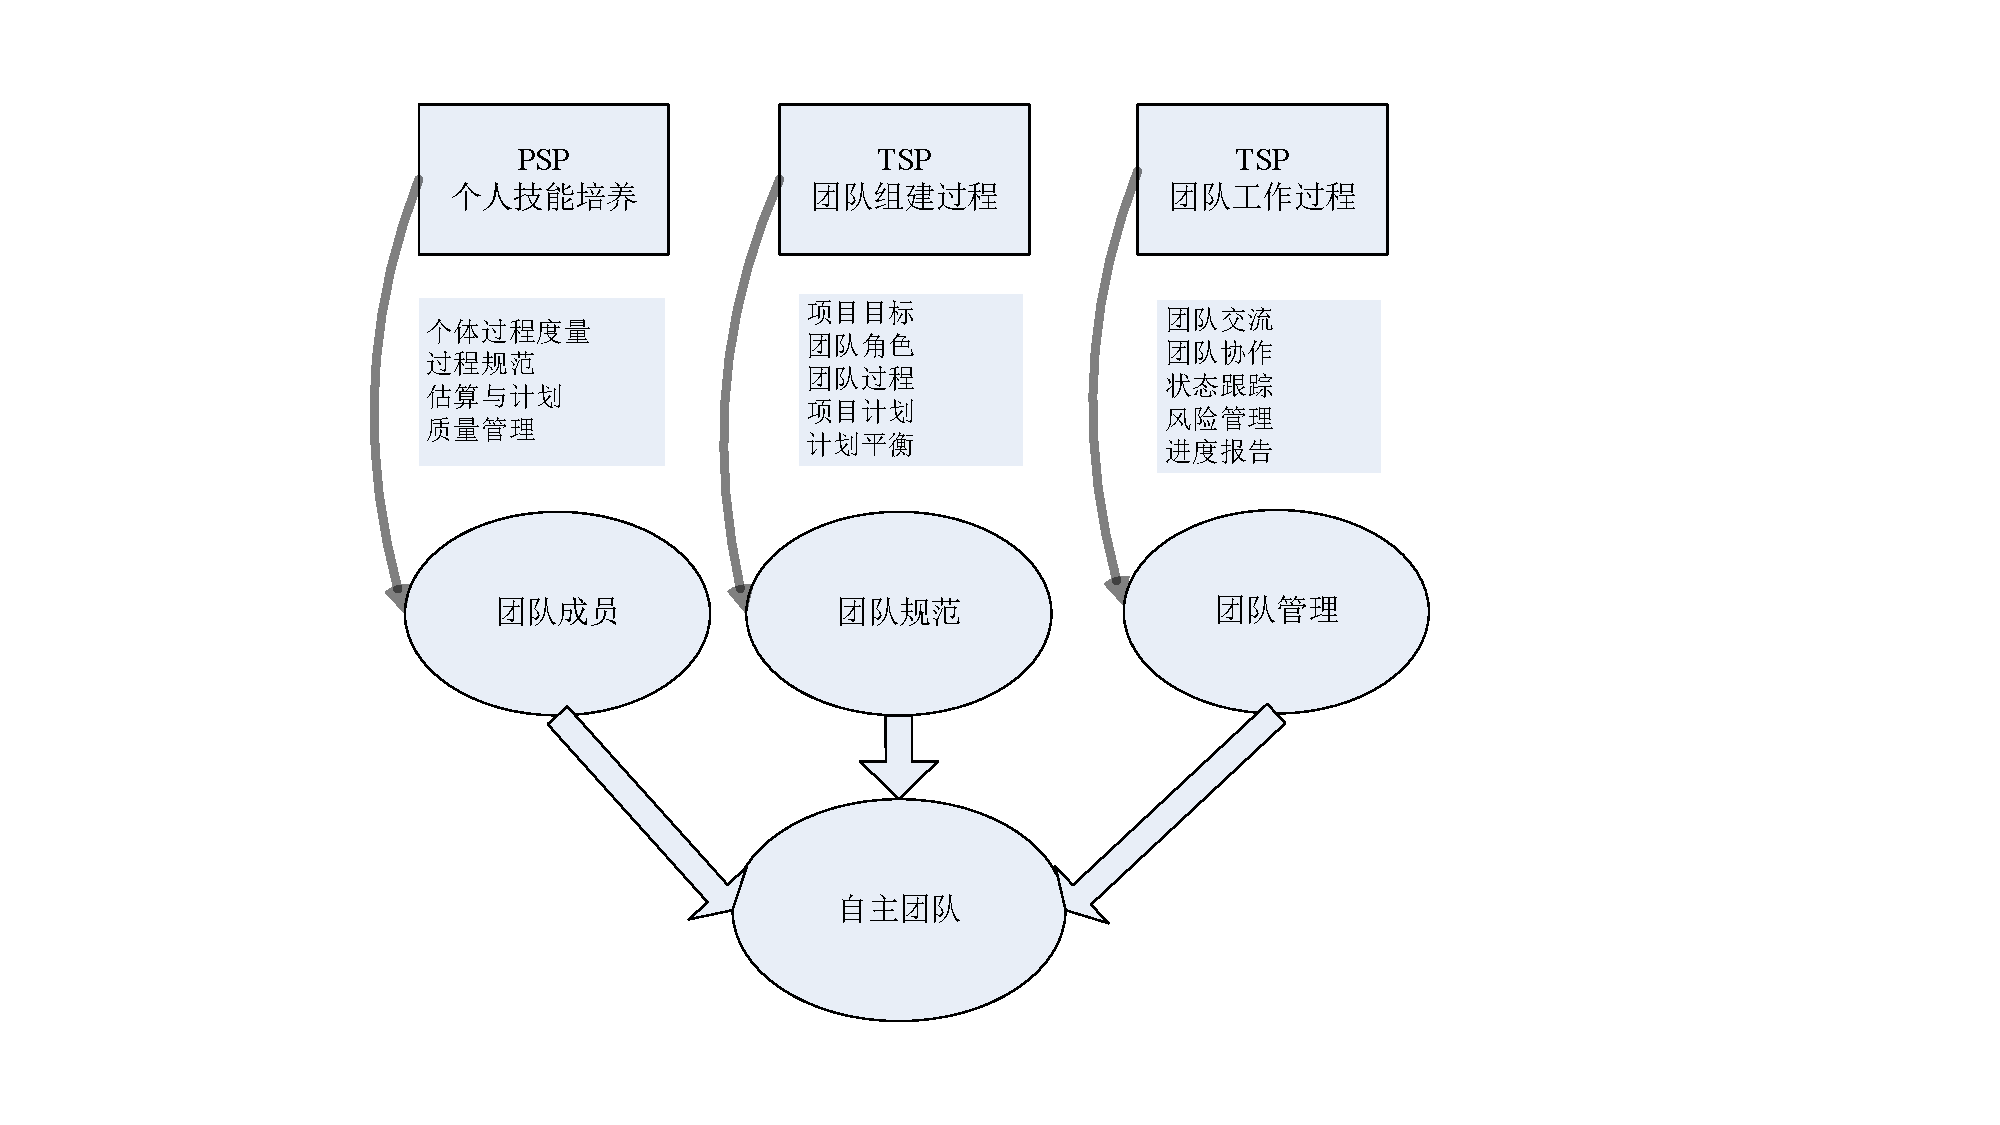
\includegraphics[width=0.6\textwidth]{images/PSP.pdf}
    \vspace{-1em}
\end{figure}
\vspace{-1em}
\end{problem}

\begin{problem}
自主团队有哪些特点?为什么说这样的团队可以满足软件开发对团队的要求?

自主团队特点如上

软件开发一种智力活动,开发者是智力劳动者,而对于智力劳动者而言,管理的第一准则就是智力劳动者不能被管理,只能实现自我管理:
\vspace{-0.8em}
\begin{multicols}{2}
    \begin{itemize}
        \item 处理和讨论非常抽象的概念
        \item 把不同的部分整合成一个可以工作的正确的系统
        \item 全身心地参与
        \item 努力做出卓越的工作
    \end{itemize}
\end{multicols}
\vspace{-1em}
\end{problem}

\begin{problem}
请结合软件开发的特点介绍软件项目管理中自主型团队的必要性以及自主团队应该具备的特征?

软件开发是一项既复杂又富有创造性的知识工作

软件开发是一种智力劳动:处理和讨论极其抽象的概念、把不同的部分(不可见)整合成一个可以工作的系统

自主团队具备如下的特点:
\vspace{-0.8em}
\begin{multicols}{2}
    \begin{itemize}
        \item 自行定义项目的目标
        \item 自行决定团队组成形式以及成员的角色
        \item 自行决定项目的开发策略
        \item 自行定义项目的开发过程
        \item 自行制定项目的开发计划
        \item 自行度量、管理和控制项目工作
    \end{itemize}
\end{multicols}
\vspace{-1em}
\end{problem}

\begin{problem}
马斯洛的“人的需求层次理论”描述的需求层次有哪几个?这样分层对软件开发有什么启发?
\end{problem}

\subsection{TSP的典型角色}
\vspace{-0.5em}
\begin{spacing}{1.2}
    \centering
    \begin{longtable}{|m{1.5cm}<{\centering}|m{4.2cm}|m{4.2cm}|m{4.2cm}|}
        \hline
        \textbf{角色} & \multicolumn{1}{c|}{\textbf{介绍}} & \multicolumn{1}{c|}{\textbf{典型技能}} & \multicolumn{1}{c|}{\textbf{工作内容}} \\ \hline
        \textbf{项目组长} & 
        项目组长的目标和衡量指标
        \begin{itemize}[leftmargin=1.3em]
            \item 建设和维持高效率的团队
            \item 激励团队成员积极工作
            \item 合理处理团队成员的问题
            \item 向管理层提供项目进度相关的完整信息
            \item 充当合格的会议组织者和协调者
            \vspace{-1.3em}
        \end{itemize} &
        \vspace{-1.1em}
        \begin{itemize}[leftmargin=1.3em]
            \item 你是天生的领导者
            \item 你有能力识别问题的关键并且做出客观的决策
            \item 你不介意偶尔充当“恶人”
            \item 你尊敬你的团队成员
            \vspace{-1.3em}
        \end{itemize} &
        \vspace{-1.1em}
        \begin{enumerate}[label=\arabic*.,leftmargin=1.5em]
            \item 激励团队成员努力工作
            \item 主持项目周例会
            \item 每周汇报项目状态
            \item 分配工作任务
            \item 维护项目资料
            \item 组织项目总结
            \vspace{-1.3em}
        \end{enumerate} \\ \hline
        \textbf{计划经理} & 
        \vspace{-1.1em}
        \begin{itemize}[leftmargin=1.3em]
            \item 开发完整的、准确的团队计划和个人计划
            \item 每周准确的报告项目小组状态
            \vspace{-1.3em}
        \end{itemize} &
        \vspace{-1.1em}
        \begin{itemize}[leftmargin=1.3em]
            \item 最为重要的一点是,你做事有条理和逻辑
            \item 你对于过程数据非常感兴趣,期待通过每周输入的数据来了解项目当前状况
            \item 你认为计划非常重要,也愿意要求团队成员跟踪和度量他们的工作
            \vspace{-1.3em}
        \end{itemize} &
        \vspace{-1.1em}
        \begin{enumerate}[label=\arabic*.,leftmargin=1.5em]
            \item 带领项目小组开发项目计划
            \item 带领项目小组平衡计划
            \item 跟踪项目进度
            \item 参与项目总结
            \vspace{-1.3em}
        \end{enumerate} \\ \hline
        \textbf{开发经理} & 
        \vspace{-1.1em}
        \begin{itemize}[leftmargin=1.3em]
            \item 开发优秀的软件产品
            \item 充分利用团队成员的技能
            \vspace{-1.3em}
        \end{itemize} &
        \vspace{-1.1em}
        \begin{itemize}[leftmargin=1.3em]
            \item 你喜欢创造事物
            \item 你愿意成为软件工程师,并且喜欢带领团队开展设计和开发工作
            \item 你具备足够的背景可以胜任设计师的工作,并且可以领导设计团队开展工作
            \item 你熟悉主流的设计工具
            \item 你愿意倾听和接受其他人的设计思想
            \vspace{-1.3em}
        \end{itemize} &
        带领团队
        \vspace{0.2em}
        \begin{enumerate}[label=\arabic*.,leftmargin=2.1em]
            \item 制定开发策略
            \item 开展产品规模估算和所需时间资源的估算
            \item 开发需求规格说明
            \item 开发高层设计
            \item 开发设计规格说明
            \item 实现软件产品
            \item 开展集成测试和系统测试
            \item 开发用户支持文档
        \end{enumerate}
        \vspace{0.3em}
        \begin{enumerate}[label=9.,leftmargin=1.5em]
            \item 参与项目总结
            \vspace{-1.3em}
        \end{enumerate} \\ \hline
        \textbf{质量经理} & 
        \vspace{-1.1em}
        \begin{itemize}[leftmargin=1.3em]
            \item 项目团队严格按照质量计划开展工作,开发出高质量的软件产品
            \item 所有的小组评审工作都正常开展,并且都形成了评审报告
            \vspace{-1.3em}
        \end{itemize} &
        \vspace{-1.1em}
        \begin{itemize}[leftmargin=1.3em]
            \item 你关注软件产品的质量
            \item 你有评审方面的经验,熟悉各种评审方法
            \item 你有协调组织有效评审的能力
            \vspace{-1.3em}
        \end{itemize} &
        \vspace{-1.1em}
        \begin{enumerate}[label=\arabic*.,leftmargin=1.5em]
            \item 带领团队开发和跟踪质量计划
            \item 向项目组长警示质量问题
            \item 软件产品提交配置管理之前,对其进行评审,以消除质量问题
            \item 项目小组评审的组织者和协调者
            \item 参与项目总结
            \vspace{-1.3em}
        \end{enumerate} \\ \hline
        \textbf{过程经理} & 
        \vspace{-1.1em}
        \begin{itemize}[leftmargin=1.3em]
            \item 所有团队成员准确的记录、报告和跟踪过程数据
            \item 所有的团队会议都有相应会议记录
            \vspace{-1.3em}
        \end{itemize} &
        \vspace{-1.1em}
        \begin{itemize}[leftmargin=1.3em]
            \item 你对过程定义、过程度量非常感兴趣
            \item 你对过程改进非常感兴趣
            \vspace{-1.3em}
        \end{itemize} &
        \vspace{-1.1em}
        \begin{enumerate}[label=\arabic*.,leftmargin=1.5em]
            \item 带领团队定义和记录开发过程并支持过程改进
            \item 建立维护团队开发标准
            \item 记录维护项目会议记录
            \item 参与项目总结
            \vspace{-1.3em}
        \end{enumerate} \\ \hline
        \textbf{支持经理} & 
        \vspace{-1.1em}
        \begin{itemize}[leftmargin=1.3em]
            \item 项目小组在整个开发过程中都有合适的工具和环境
            \item 对于基线产品,不存在非授权的变更
            \item 项目小组的风险和问题得到跟踪
            \item 项目小组在开发过程中满足复用目标
            \vspace{-1.3em}
        \end{itemize} &
        \vspace{-1.1em}
        \begin{itemize}[leftmargin=1.3em]
            \item 你对于各种开发工具很感兴趣,熟悉各类工具的适用场合
            \item 你对版本控制工具很熟悉,也熟悉配置管理流程
            \item 对于本项目所有工具而言,你都是专家
            \vspace{-1.3em}
        \end{itemize} &
        \vspace{-1.1em}
        \begin{enumerate}[label=\arabic*.,leftmargin=1.5em]
            \item 带领团队识别开发过程中所需各类工具和设施
            \item 主持配置管理委员会,管理配置管理系统
            \item 维护软件项目的词汇表
            \item 维护项目风险和问题跟踪系统
            \item 支持软件开发过程中复用策略的应用
            \item 参与项目总结
            \vspace{-1.3em}
        \end{enumerate}\\ \hline
        \textbf{开发人员} & \multicolumn{1}{c|}{—} & \multicolumn{1}{c|}{—} & \multicolumn{1}{c|}{—} \\ \hline
    \end{longtable}
\end{spacing}
\vspace{-5em}


\begin{problem}
TSP项目经理、过程经理、计划经理的工作内容、项目总结角度
\end{problem}

\begin{problem}
	下列描述当中,属于过程经理的工作内容有哪些?
	\uline{AC}    
    \vspace{-0.8em}
    \begin{multicols}{2}
        \begin{enumerate}[label=\Alph*.]
            \item 建立团队的开发标准
            \item 主持项目周例会
            \item 记录周例会的会议记录
            \item 制定开发计划
        \end{enumerate}
    \end{multicols}
    \vspace{-1em}
\end{problem}
	\section{定量管理与仿真建模}

\subsection{定量管理}
\begin{figure}[H]
    \vspace{-0.5em}
	\centering
	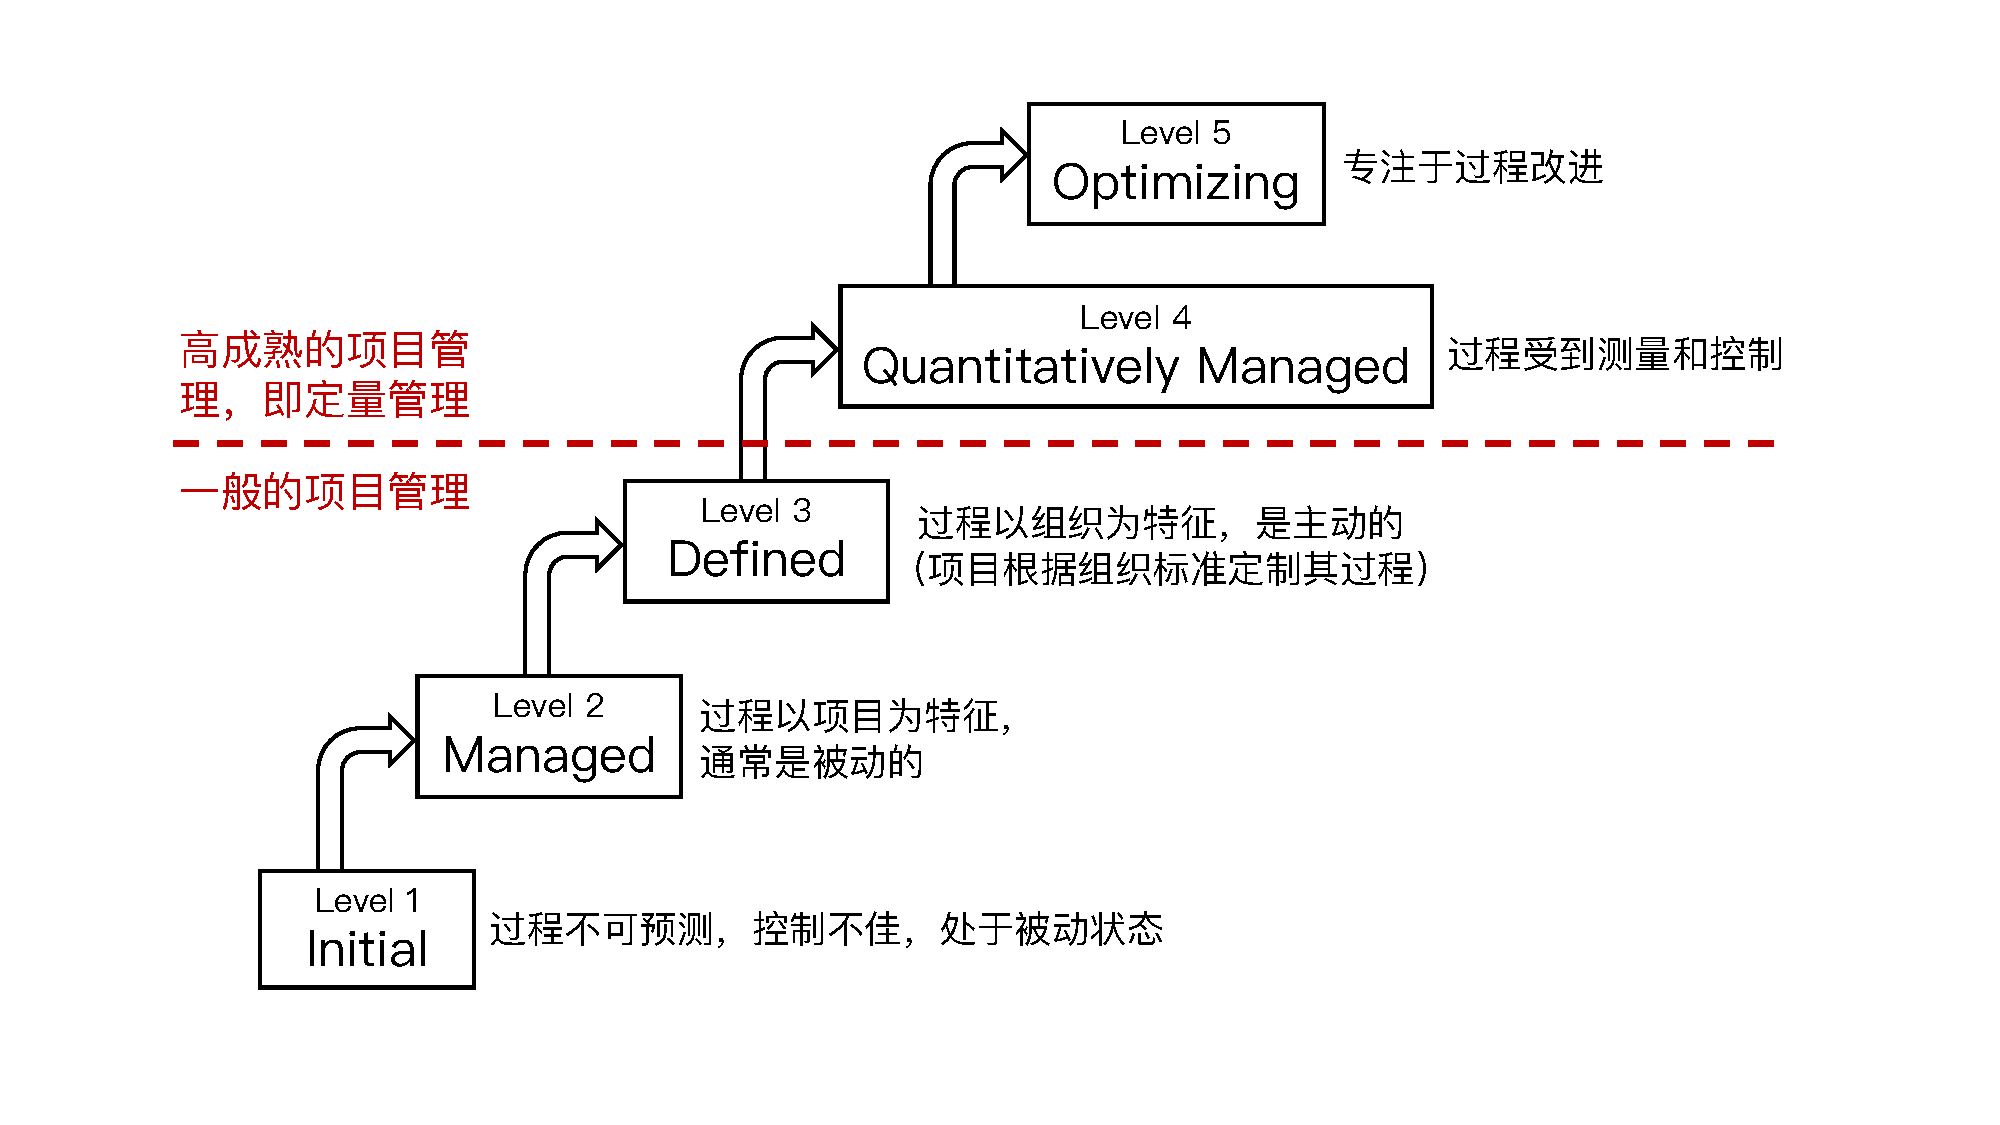
\includegraphics[width=0.75\textwidth]{images/高成熟度项目管理.pdf}
    \vspace{-1em}
\end{figure}

\subsubsection{一般的项目管理}
主要关心
\vspace{-0.8em}
\begin{multicols}{2}
    \begin{itemize}
        \item 当前状况(注意:也可能使用数据)
        \item 是否需要调整干预
    \end{itemize}
\end{multicols}
\vspace{-1em}

但是,回答不了必须进行预测的问题,例如
\vspace{-0.8em}
\begin{multicols}{2}
    \begin{itemize}
        \item 维持现状,项目最后是否能成功?
        \item 如果某些方面进行调整,会有什么不同的结果?
    \end{itemize}
\end{multicols}
\vspace{-1em}

\subsubsection{定量的项目管理}
基于数据,主要关心
\vspace{-0.8em}
\begin{multicols}{2}
    \begin{itemize}
        \item 你对当前状态理解是否有足够信心?
        \item 对偏差的理解
    \end{itemize}
\end{multicols}
\vspace{-1em}

回答如下典型问题
\vspace{-0.8em}
\begin{multicols}{2}
    \begin{itemize}
        \item 项目最后能否成功?多大把握?是否需要预防?
        \item 如果某些方面进行调整,会有什么不同的结果?
    \end{itemize}
\end{multicols}
\vspace{-1em}

\subsubsection{为什么需要理解偏差}
有的时候,我们会面临这样的问题:客户希望10周以内交付,但是,历史数据表明,类似任务是$9\sim 11$周完成,那这个任务该接受么?
\begin{figure}[H]
    \vspace{-0.5em}
	\centering
	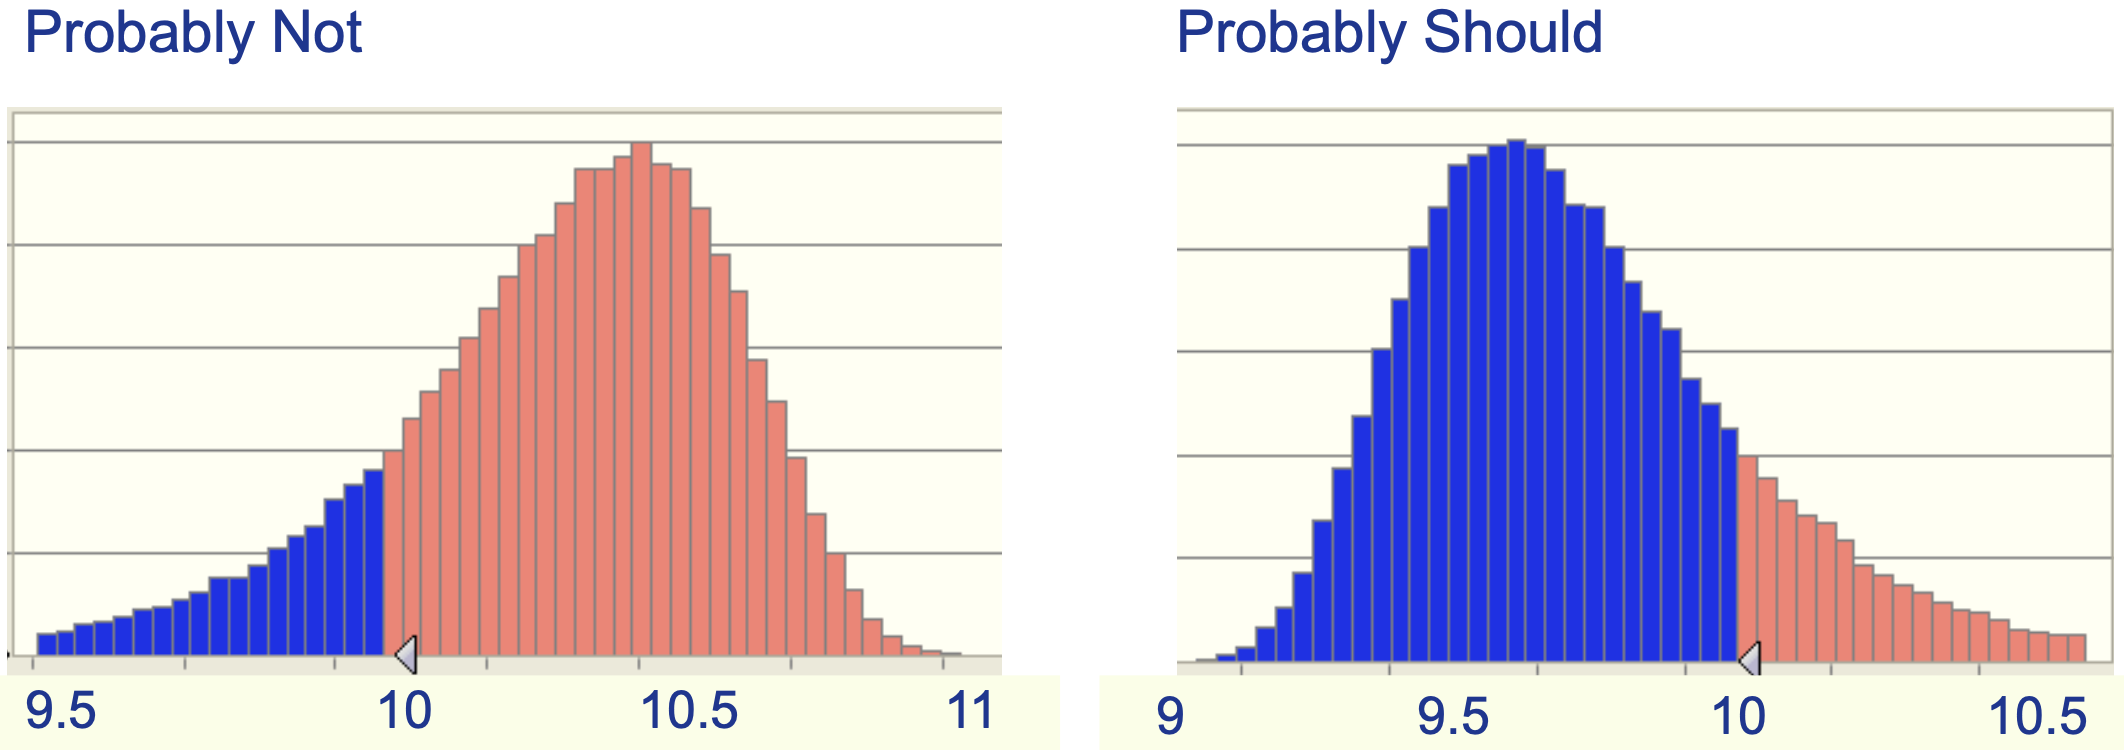
\includegraphics[width=0.75\textwidth]{images/为什么需要理解偏差.png}
    \vspace{-1em}
\end{figure}

\subsubsection{定量管理基本范式}
构建定量模型
\vspace{-0.8em}
\begin{multicols}{2}
    \begin{itemize}
        \item 子过程能力基线
        \item 过程模型
    \end{itemize}
\end{multicols}
\vspace{-1em}

应用模型:监控影响子过程的关键因素

\subsubsection{基本概念}
\begin{itemize}
    \item (子)过程性能:遵循某个特定(子)过程的之后产生结果的量化描述,既包括(子)过程度量Xi(例如,时间、缺陷消除效率、工时等),也包括产物度量Yi(例如,缺陷密度,相应时间等)
    \item (子)过程性能基线:上述过程性能的一个定量化的刻画,一般包括均值和范围。通常用作过程性能的benchmark
    \item 过程或子过程性能模型:依据子过程的逻辑关系构建相应的数学模型,描述子过程性能基线和整体过程有意义的性能输出(例如,质量、生产效率、成本等)之间关系。例如过程Yield和Phase Yield
\end{itemize}

\subsubsection{定量模型构建的关键实践}
\begin{figure}[H]
	\setcounter{subfigure}{0}
	\centering
	\vspace{-0.5em}	
	\subfloat{
	\begin{minipage}[t]{0.5\linewidth}
	\centering
	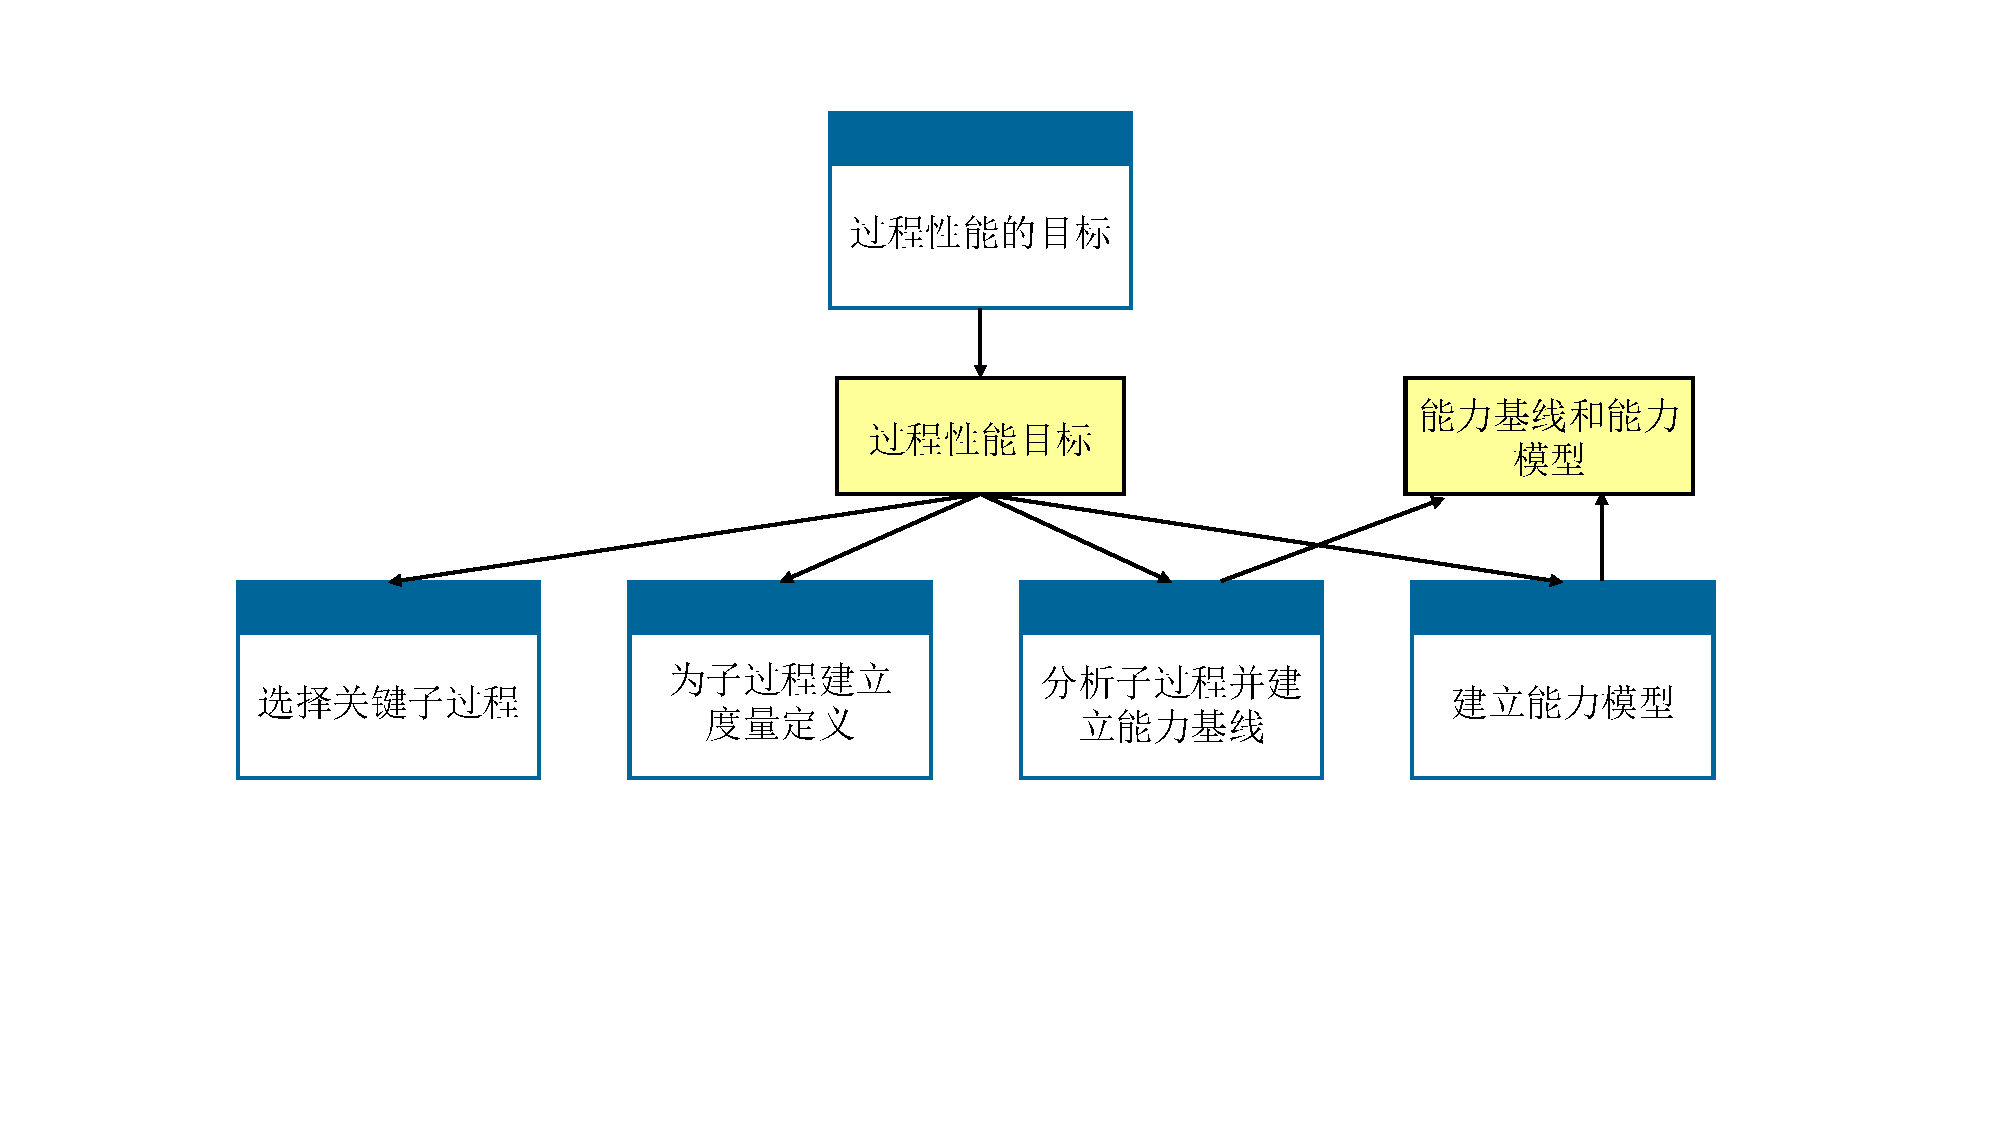
\includegraphics[width=\textwidth]{images/定量模型构建的关键实践.pdf}
	\end{minipage}
	}
	\subfloat{
	\begin{minipage}[t]{0.49\linewidth}
	\centering
	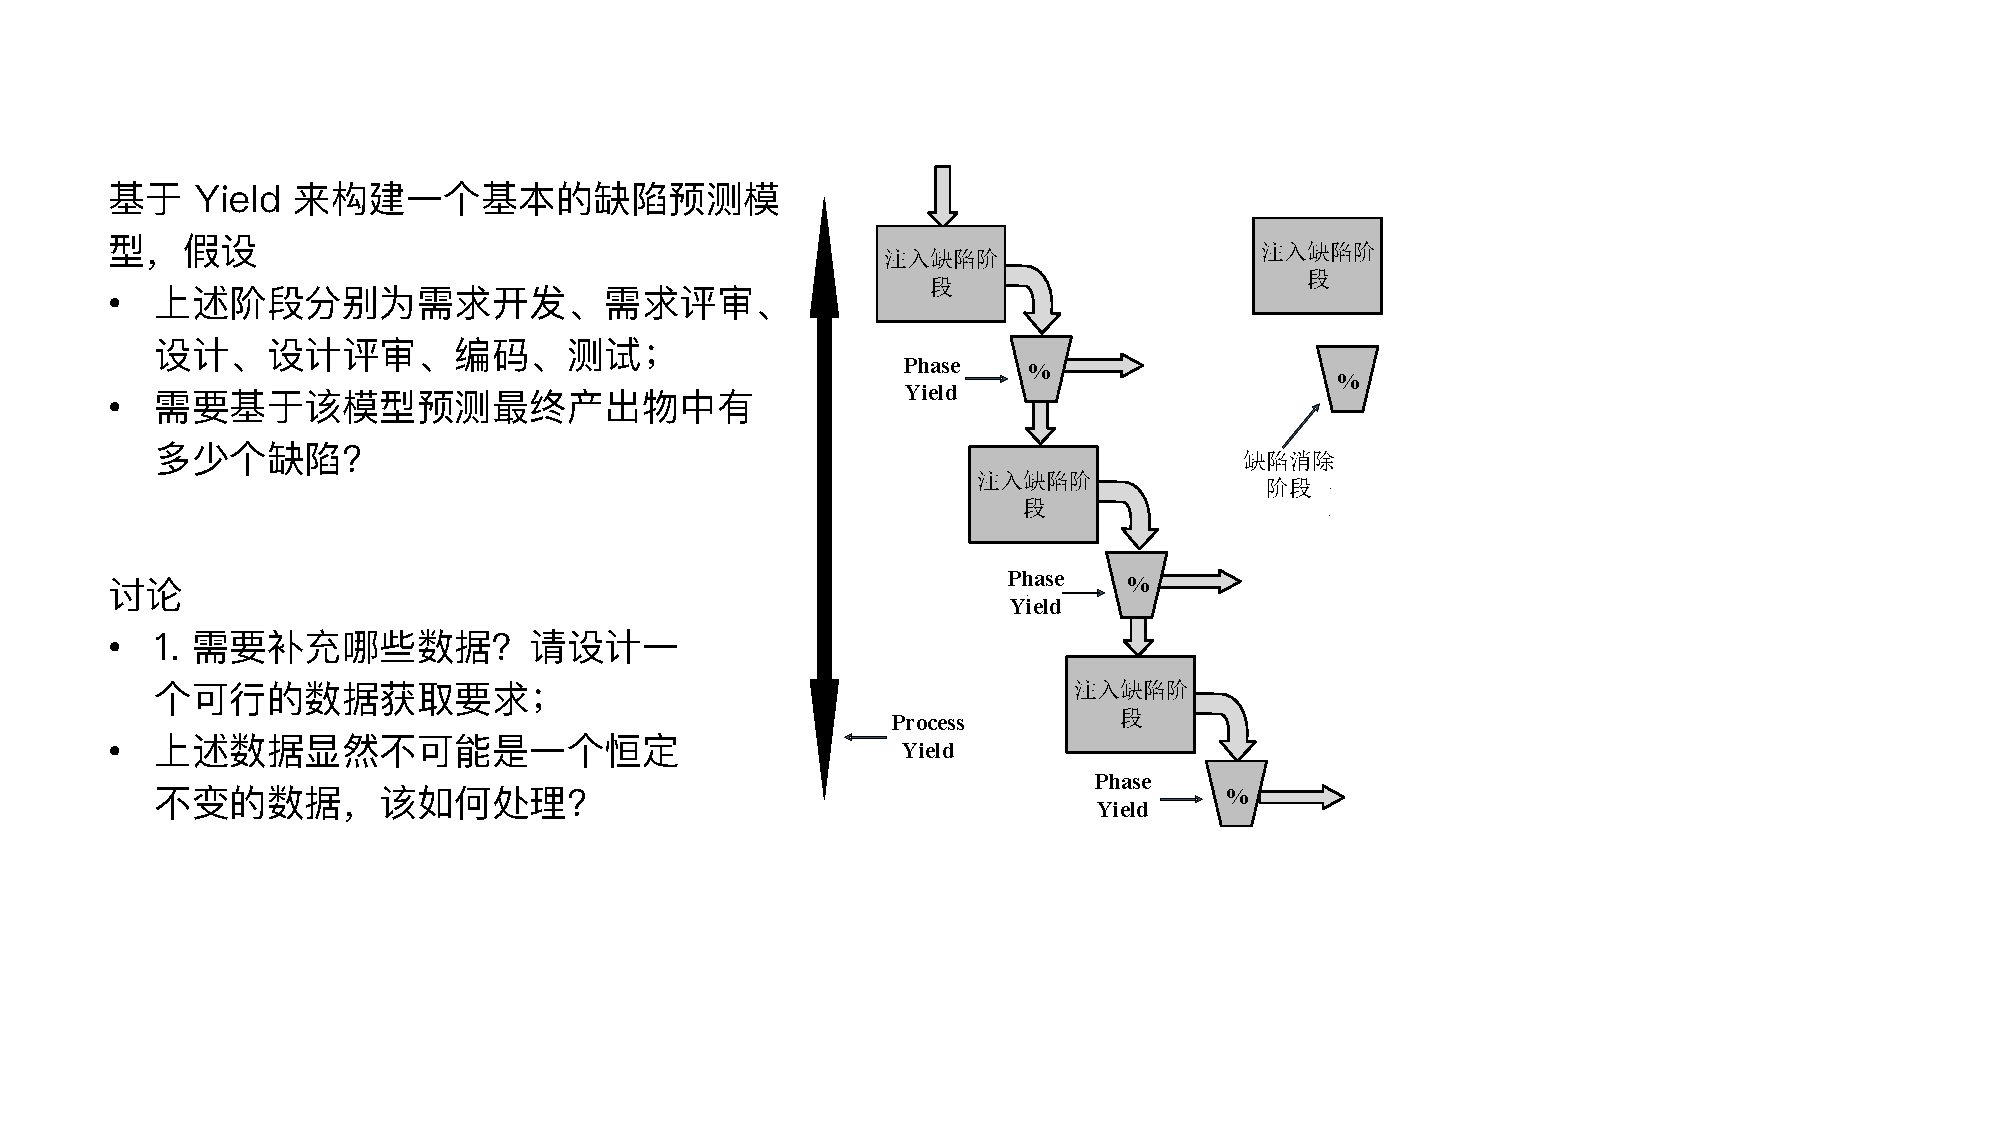
\includegraphics[width=\textwidth]{images/定量模型构建的关键实践练习.pdf}
	\end{minipage}
	}
	\centering
    \vspace{-1em}
\end{figure}

\subsubsection{定量模型应用(定量管理)的关键实践}
\begin{figure}[H]
    \vspace{-0.5em}
	\centering
	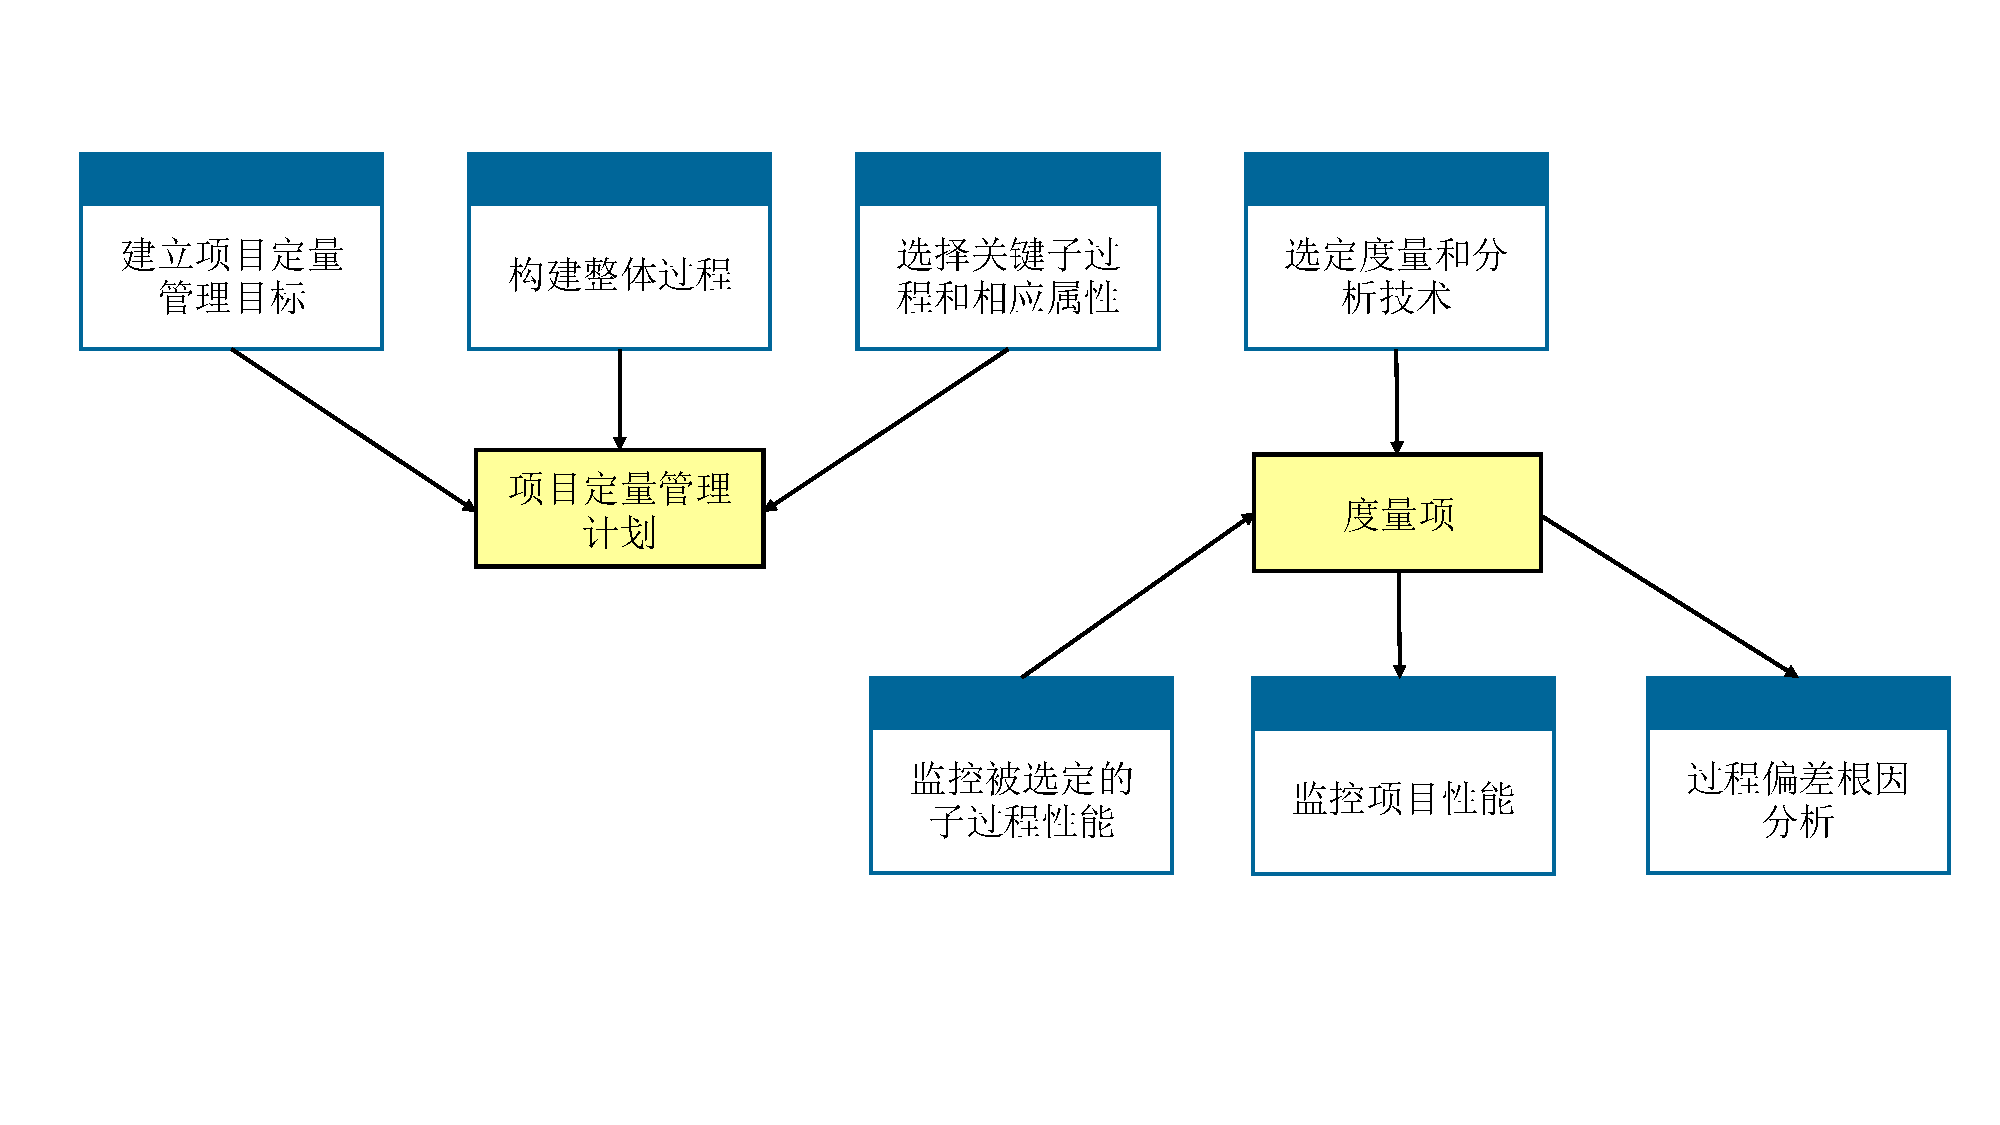
\includegraphics[width=0.9\textwidth]{images/定量模型应用(定量管理)的关键实践.pdf}
    \vspace{-1em}
\end{figure}

\subsection{常用定量管理技术}
定量管理技术通常被分为\textbf{非统计技术}和\textbf{统计技术},这些技术的使用能帮助解决软件项目管理中多种问题

\subsubsection{常用非统计技术}
非统计技术一般是为了描述数据集整体特征或者关联关系,从而帮助选择适用的统计技术以应用于给定的数据集,以及调查通过数据分析检测到异常的原因。例如,检查表(或列联表),帕累托图,直方图,因果图,散点图等。


\paragraph{直方图}~{} \par
直方图以频率统计的方式进行显示,可以描述过程属性的频率,例如缺陷修复的时间、每次测试发现的缺陷的个数、每天无故障工作的时间、计算产品的不合格率等

一般用于有助于判断过程是否正常,过程能力是否满足需要,不良产品是否发生,分析产品质量问题的原因等
\begin{figure}[H]
	\setcounter{subfigure}{0}
	\centering
	\vspace{-0.5em}	
	\subfloat[案例1:人力资源分配直方图]{
	\begin{minipage}[t]{0.47\linewidth}
	\centering
	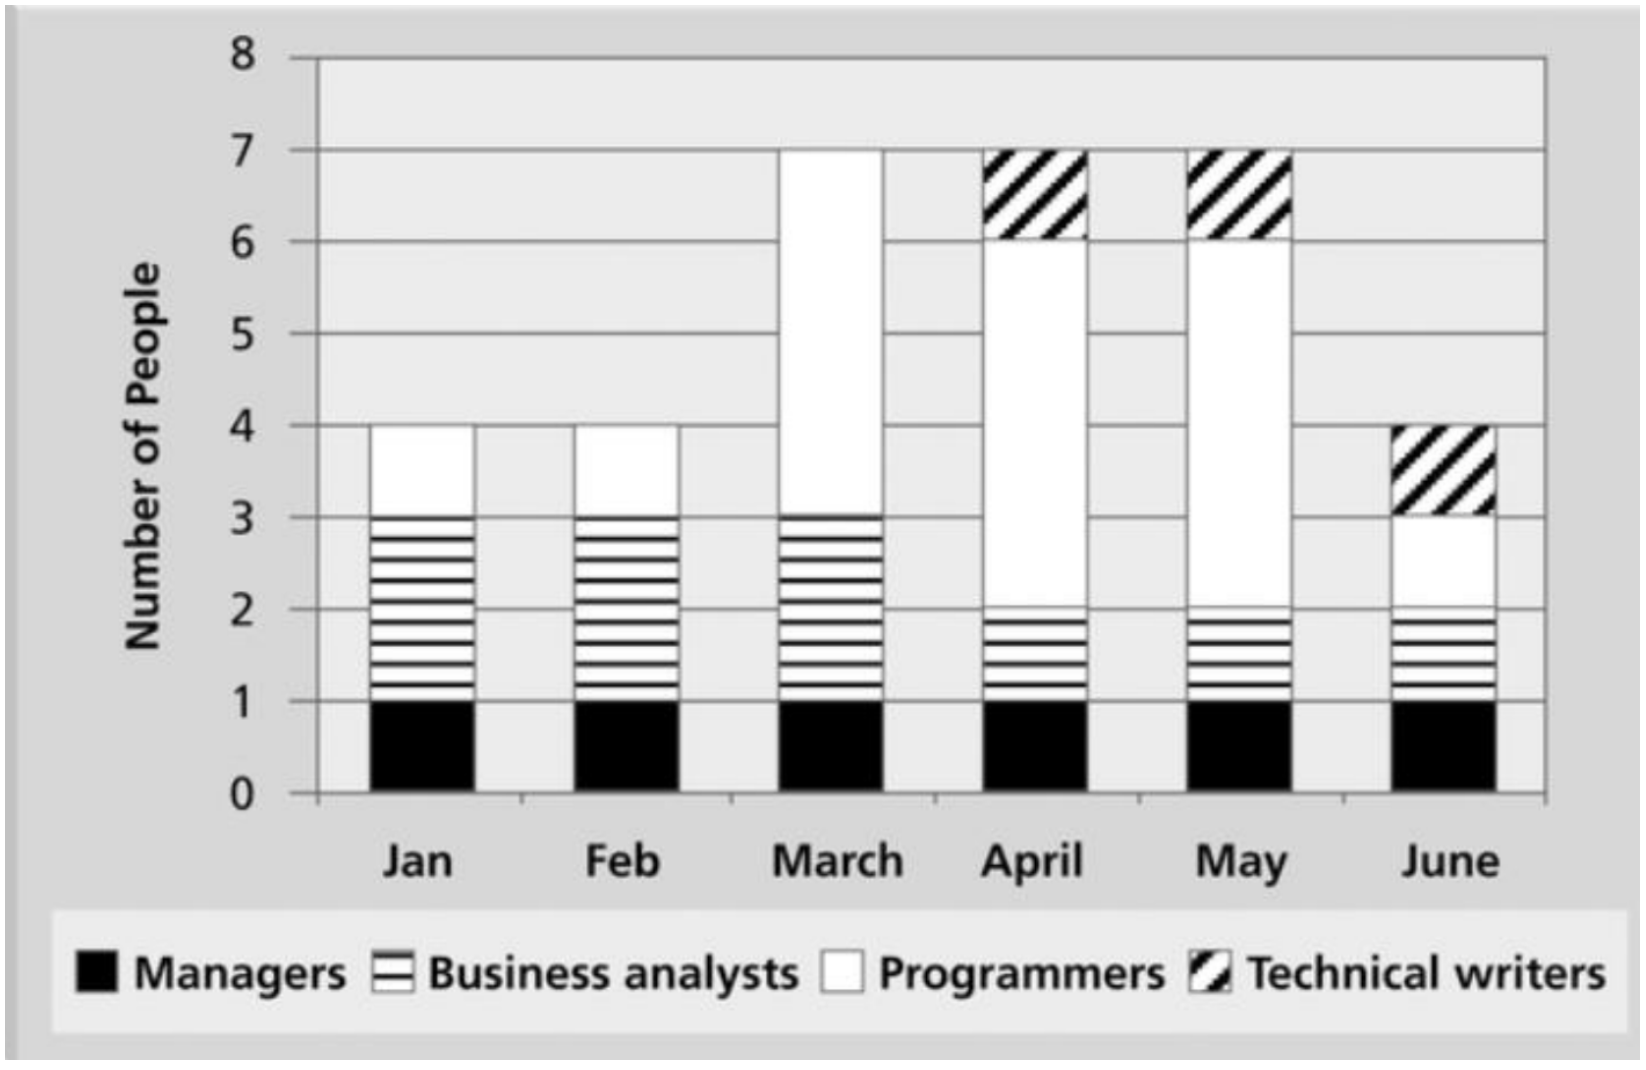
\includegraphics[width=\linewidth]{images/人力资源分配直方图.png}
	\end{minipage}
	}
	\subfloat[案例2:缺陷占比直方图]{
	\begin{minipage}[t]{0.47\linewidth}
	\centering
	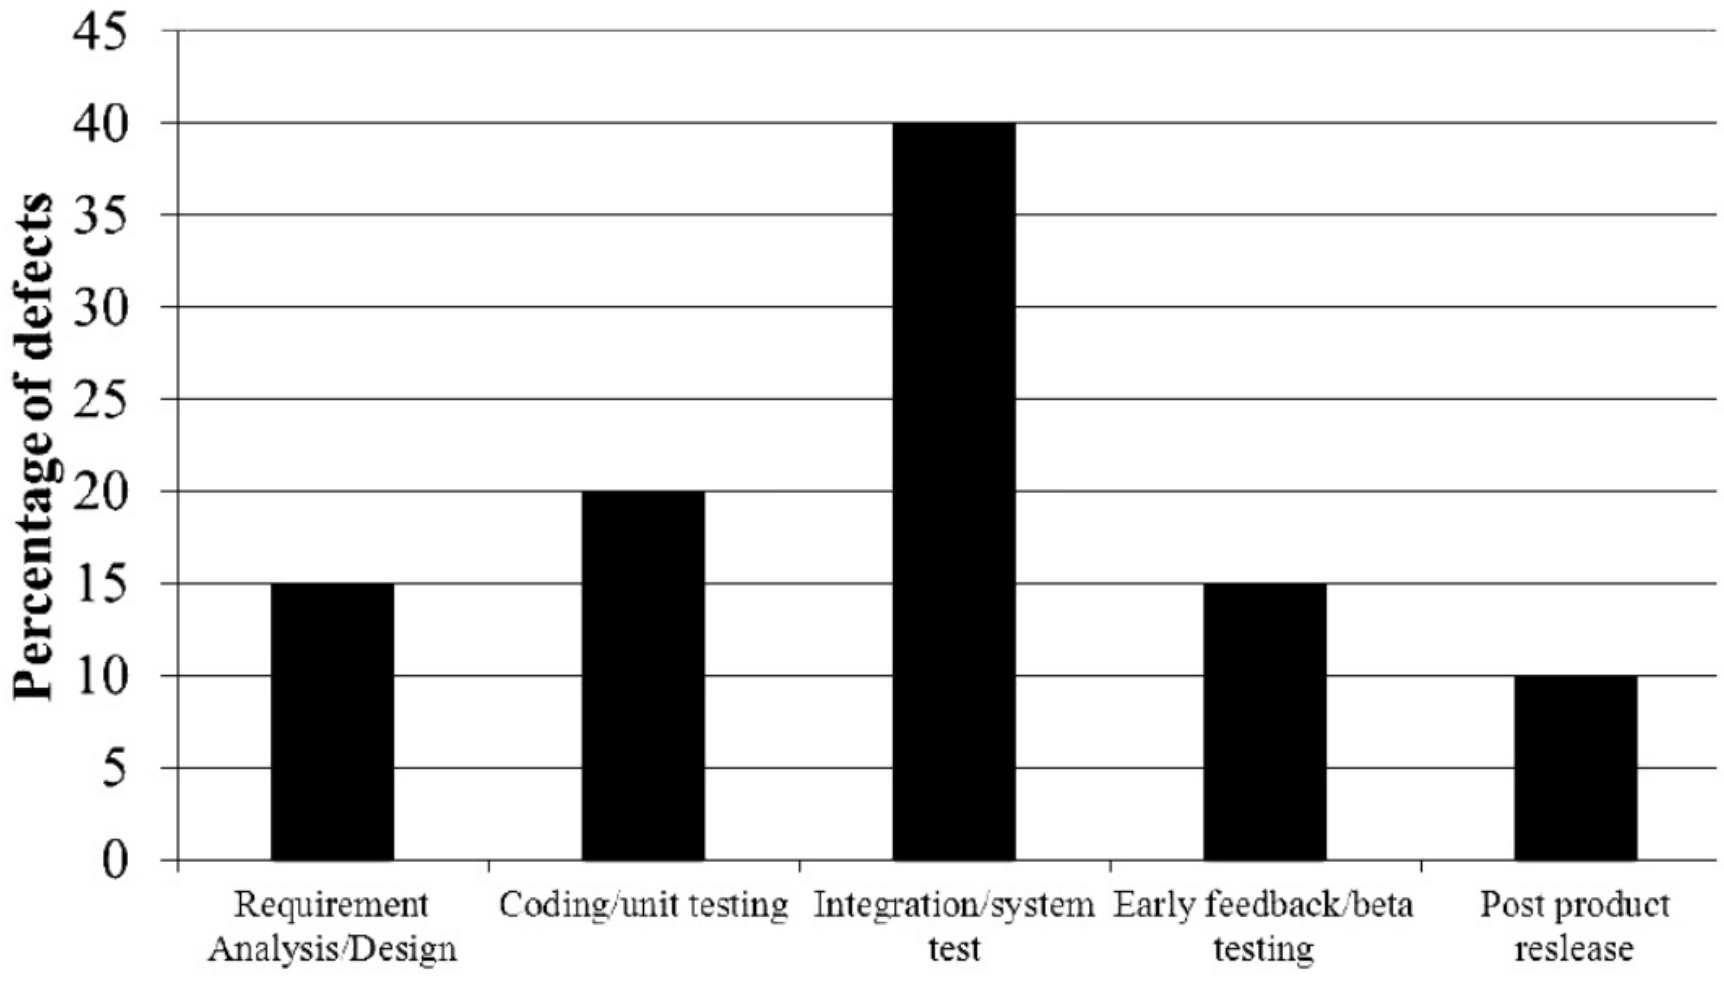
\includegraphics[width=\linewidth]{images/缺陷占比直方图.png}
	\end{minipage}
	}
	\centering
    \vspace{-1em}
\end{figure}

\paragraph{帕累托图}~{} \par
\vspace{-0.8em}
\begin{multicols}{2}
    \begin{itemize}
        \item 一种特殊的直方图
        \item 按照由高到低排列的直方图
    \end{itemize}
\end{multicols}
\vspace{-1em}

\begin{wraptable}{r}{0.33\textwidth}
    \centering
    \vspace{-1.7em}
    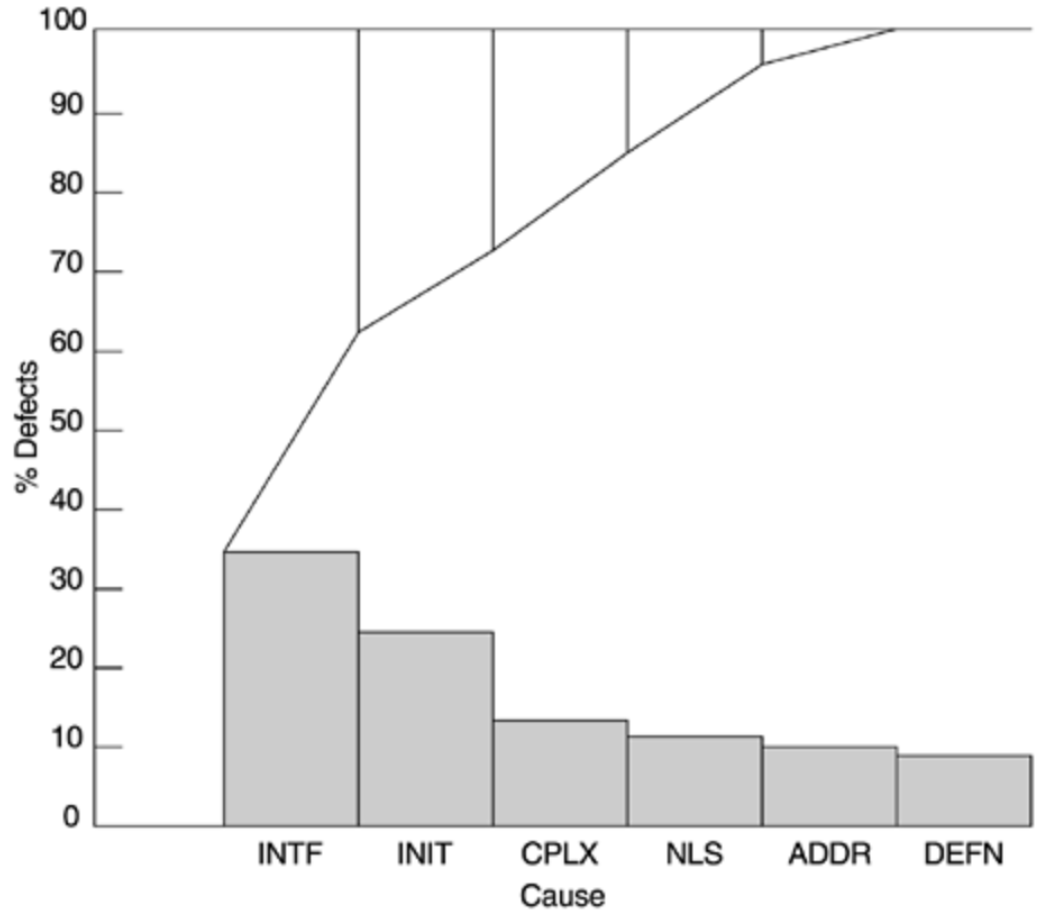
\includegraphics[width=0.33\textwidth]{images/帕累托图示例.png}
    \vspace{-4em}
\end{wraptable}
案例:如图显示了IBM Rochester产品缺陷原因的帕累托分析示例。发现接口问题(INTF)和数据初始化问题(INIT)是该产品缺陷的主要原因。通过在整个设计,实施和测试过程中专注于这两个领域,并通过同行专家进行技术培训,可以观察到明显的改进。图中的其他缺陷原因包括复杂的逻辑问题(CPLX),与翻译有关的本国语言问题(NLS),与地址有关的问题(ADDR)和数据定义问题(DEFN)。

\paragraph{因果图}~{} \par
因果图是用来分析影响产品质量的各种原因的一种有效的定性的分析图,它将对特性或结果有影响的要素加以分类分析,是一种发现问题根本原因的方法,可以让项目组成员通过头脑风暴、集思广益的方法从各个方面各种不同的角度找出这些问题的所有原因

\begin{wraptable}{r}{0.55\textwidth}
    \centering
    \vspace{-1.5em}
    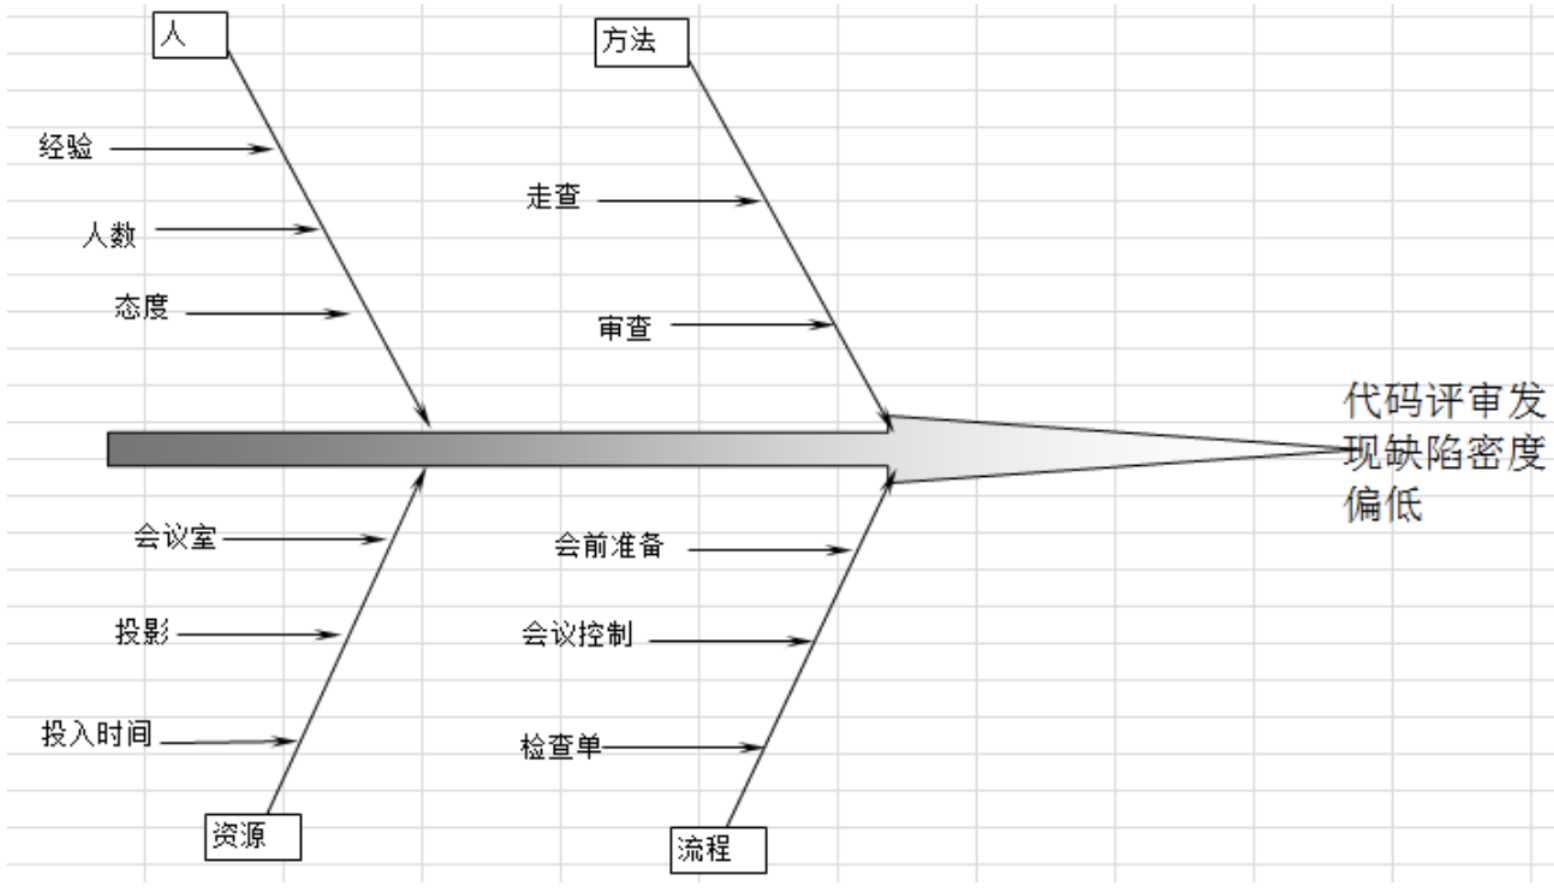
\includegraphics[width=0.55\textwidth]{images/因果图示例.png}
    \vspace{-4em}
\end{wraptable}
案例:某公司发现代码评审时发现的缺陷密度较低,使用因果图分析得知影响评审结果的因素有硬件资源、流程、方法、人员等。深入的调查发现此项目工期、规模都是稳定的,开发人员的工作环境和硬件资源也是固定的,且项目组人员也严格遵守了组织订立的过程和方法,但是项目进行代码评审的人员都是缺少开发经验的新人,这可能是导致代码评审发现的缺陷数偏少的根本原因。

\paragraph{散布(点)图}~{} \par
整理和观察收集到的数据的常用图形工具:散布图表示的是一个变量相对于另一个变量的表现情况,可以假定一个变量是因变量,另一个变量是自变量。散布图通常表现了5种相关关系。如图所示的散布图中分别表现了两个变量之间的弱正相关、弱负相关、不相关、强正相关、强负相关。
\begin{figure}[H]
    \vspace{-0.5em}
	\centering
	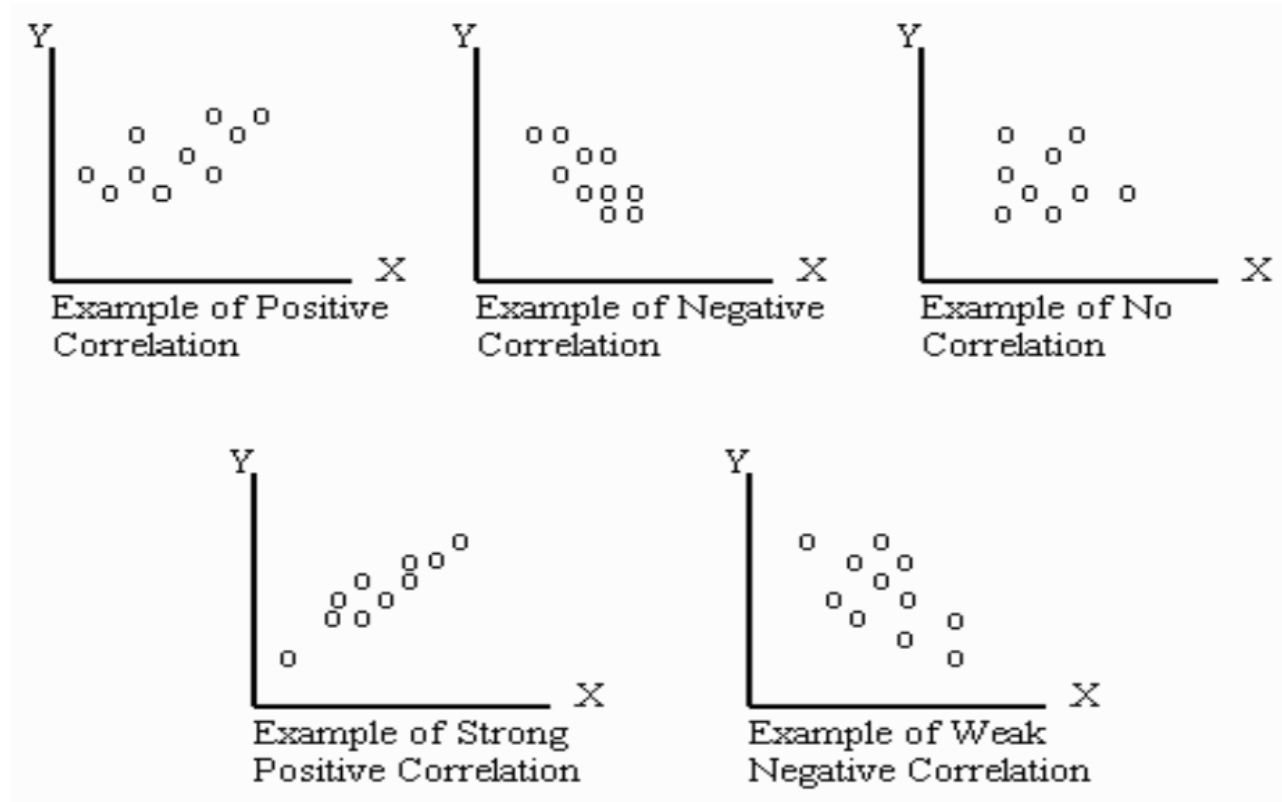
\includegraphics[width=0.6\textwidth]{images/散布图.png}
    \vspace{-1em}
\end{figure}

\subsubsection{常用统计技术}
\begin{itemize}
    \item 统计思维认识到许多决策是在\textbf{不确定条件}下做出的。统计方法有助于\textbf{量化这种不确定性}并指导采取行动以减少不确定性
    \item 统计分析支持许多类型的决策,在支持过程管理决策的统计分析中,有效的过程管理通常需要两级决策
    \begin{itemize}
        \item 实时控制单个活动或子流程
        \item 根据当前和已完成的活动对未来和最终过程的结果进行预测
    \end{itemize}
    \item 常用的统计技术包括:\textbf{统计过程控制图,回归分析,方差分析,预测区间,假设检验,敏感性分析}等
\end{itemize}


\paragraph{控制图}~{} \par
\begin{itemize}
    \item 控制图是根据概率统计原理构造的一种图,用来监测生产过程是否处于控制状态
    \item 控制图是对过程质量数据测定、记录从而进行质量管理的一种用科学方法设计的图
    \item 图上有\textbf{中心线}(CL)、\textbf{上控制限}(UCL)和\textbf{下控制限}(LCL),并有按时间顺序抽取的样本统计量数值的描点序列
\end{itemize}

\begin{figure}[H]
    \vspace{-0.5em}
	\centering
	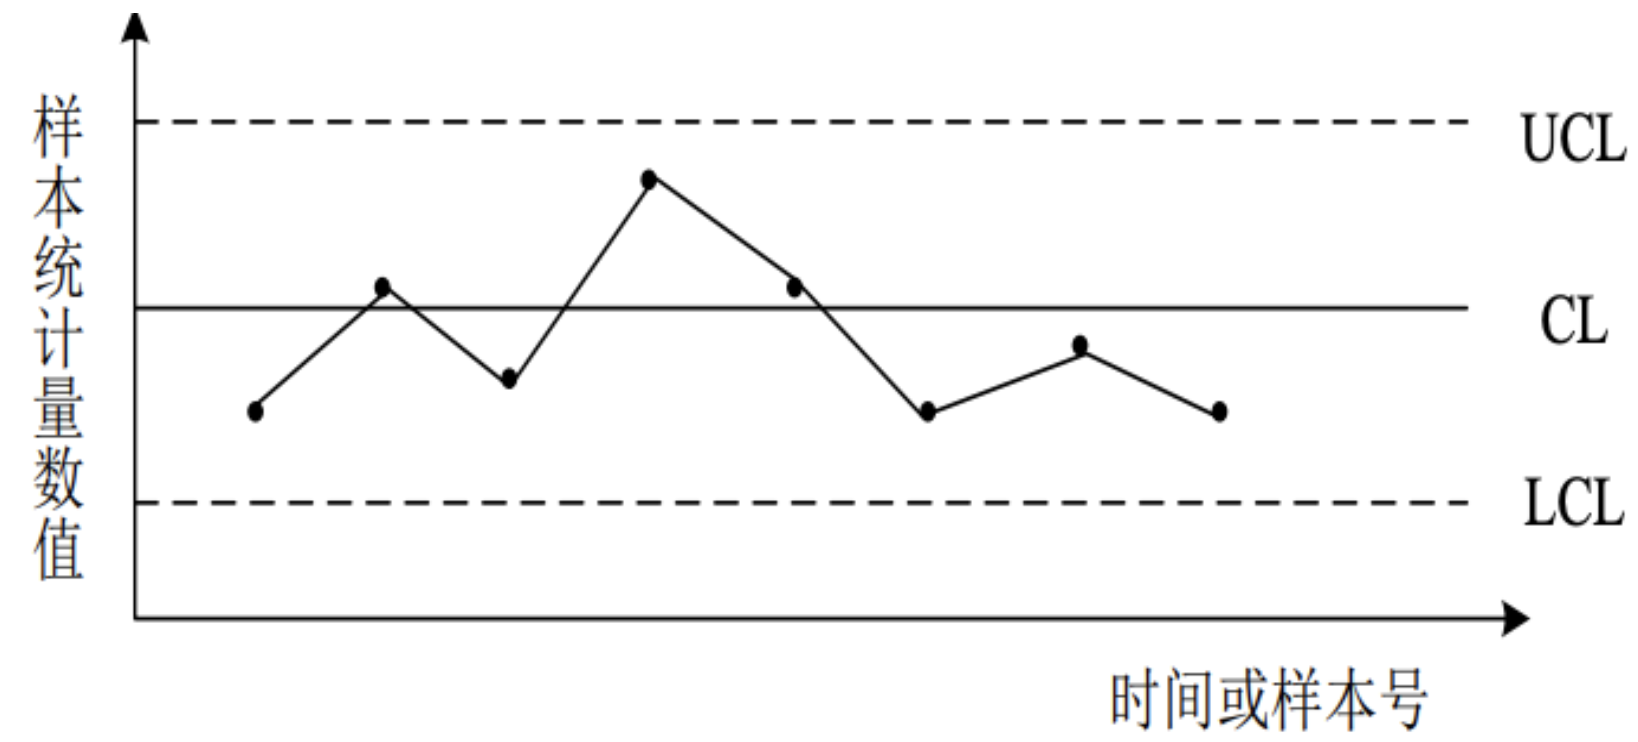
\includegraphics[width=0.55\textwidth]{images/控制图.png}
    \vspace{-1em}
\end{figure}

\begin{wraptable}{r}{0.55\textwidth}
    \centering
    \vspace{-1.5em}
    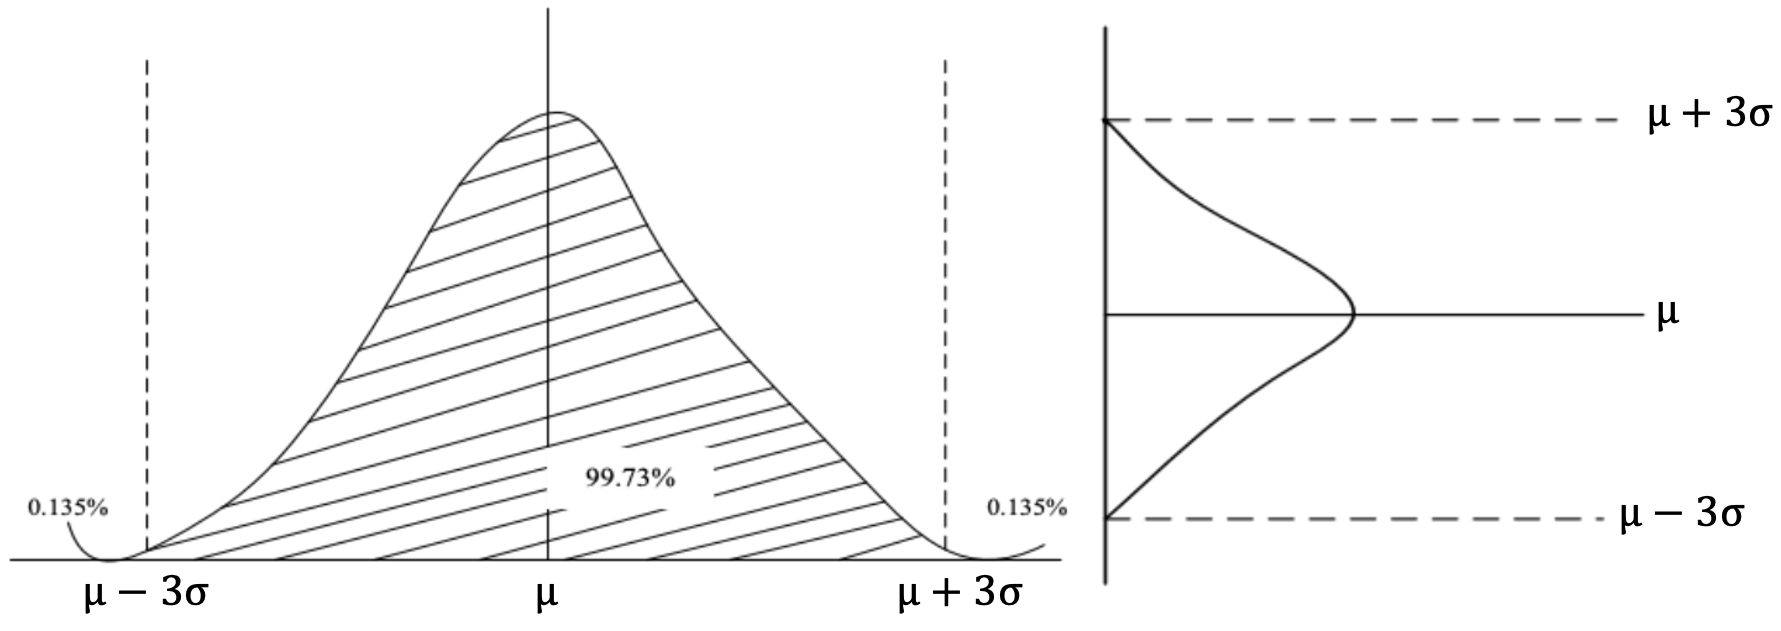
\includegraphics[width=0.55\textwidth]{images/正态分布.png}
    \vspace{-2.5em}
\end{wraptable}
控制图可由正态分布演变而来:正态分布可用两个参数即均值$\mu$和标准差$\sigma$来决定。正态分布有一个结论对质量管理很有用,即无论均值$\mu$和标准差$\sigma$取何值,产品质量特性值落在$\mu \pm 3\sigma$之间的概率为99.73\%,落在$\mu \pm 3\sigma$之外的概率为$100\% - 99.73\% = 0.27\%$,而超过一侧,即大于$\mu + 3\sigma$或小于$\mu - 3\sigma$的概率为$0.27\%/2=0.135\% \approx 1\text{\textperthousand}$。

以下显示了不处于受控状态的8种典型情况(异常模式):
\begin{figure}[H]
	\setcounter{subfigure}{0}
	\centering
	\vspace{-0.5em}	
	\subfloat{
	\begin{minipage}[t]{0.47\linewidth}
	\centering
	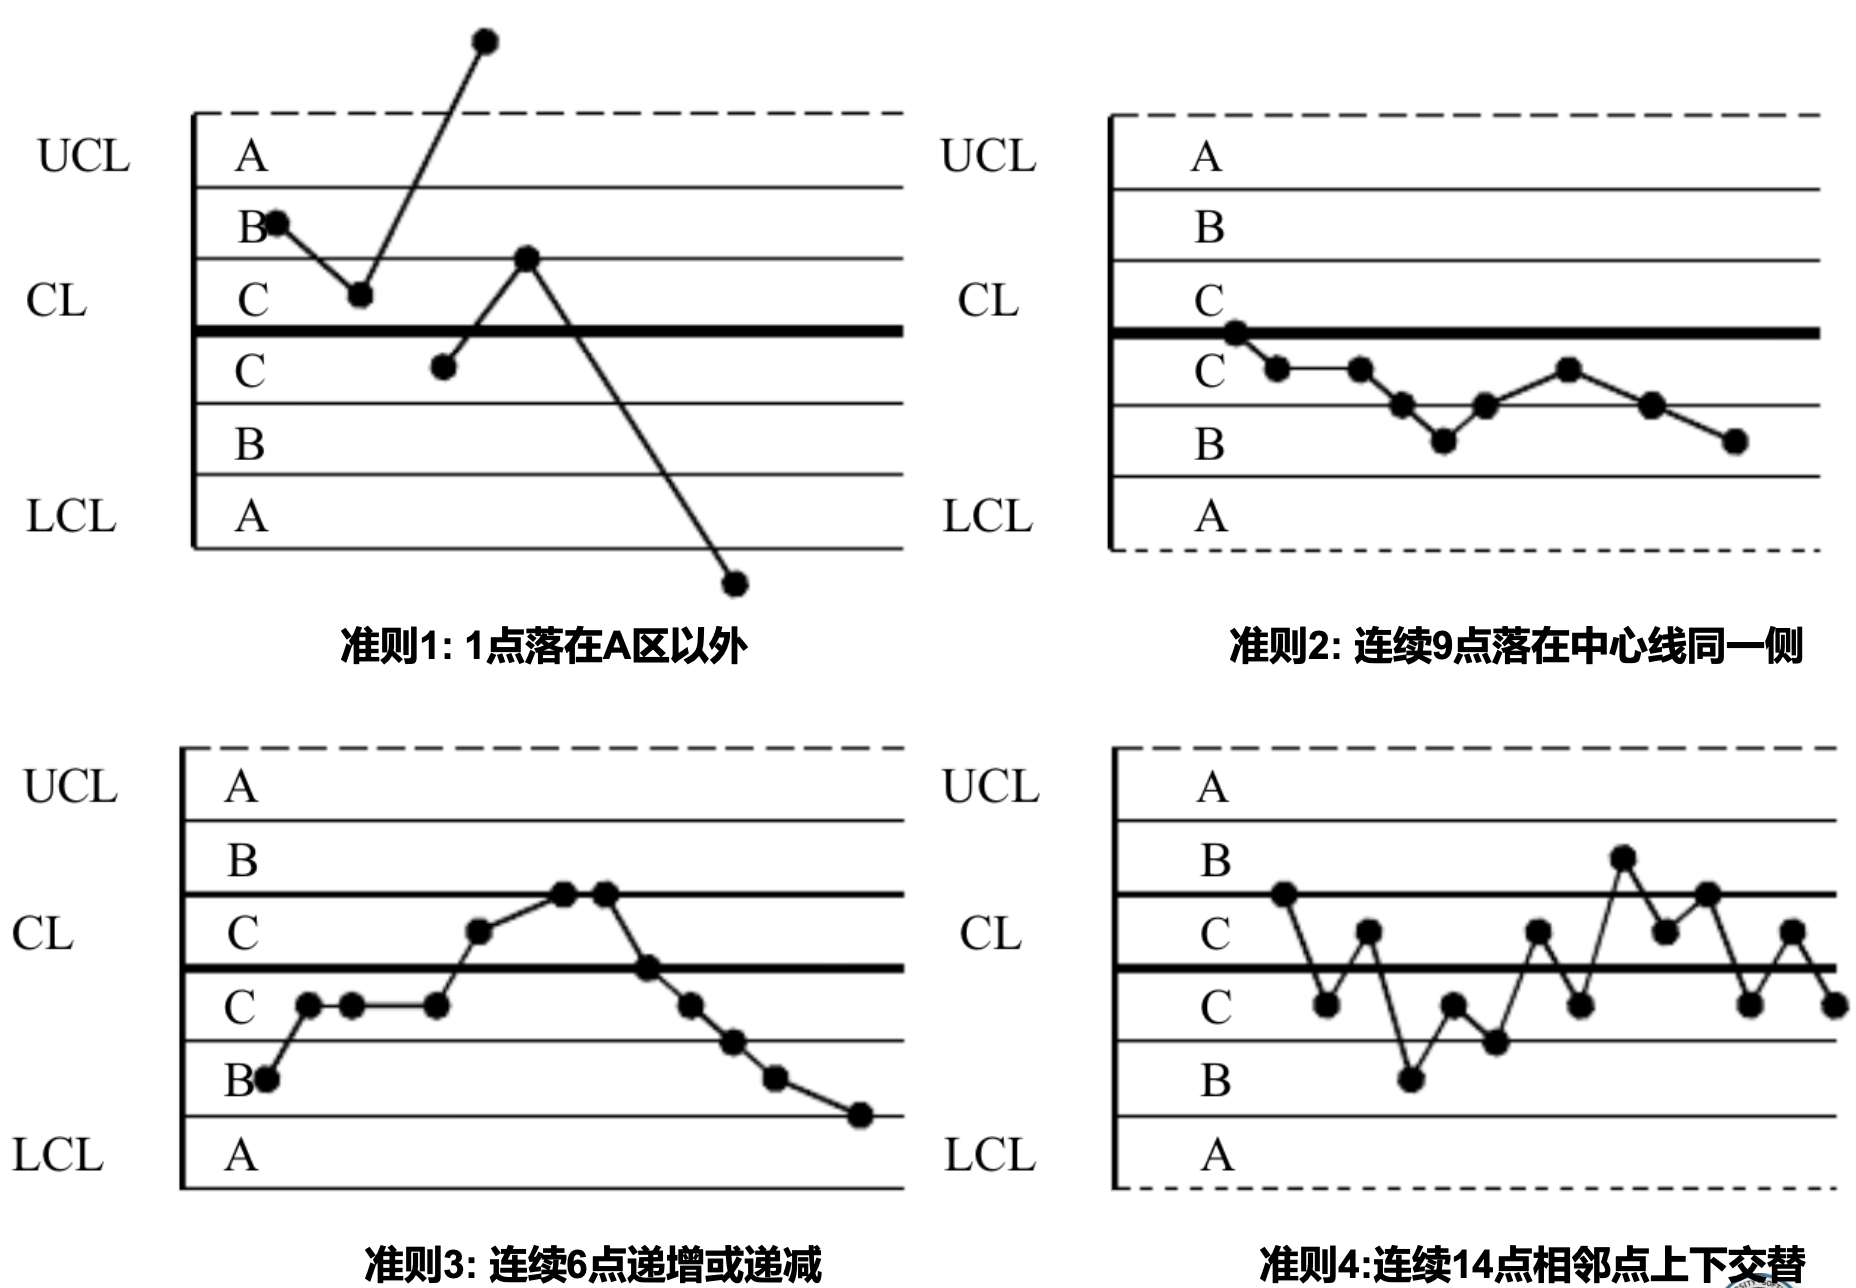
\includegraphics[width=\linewidth]{images/异常模式1.png}
	\end{minipage}
	}
	\subfloat{
	\begin{minipage}[t]{0.47\linewidth}
	\centering
	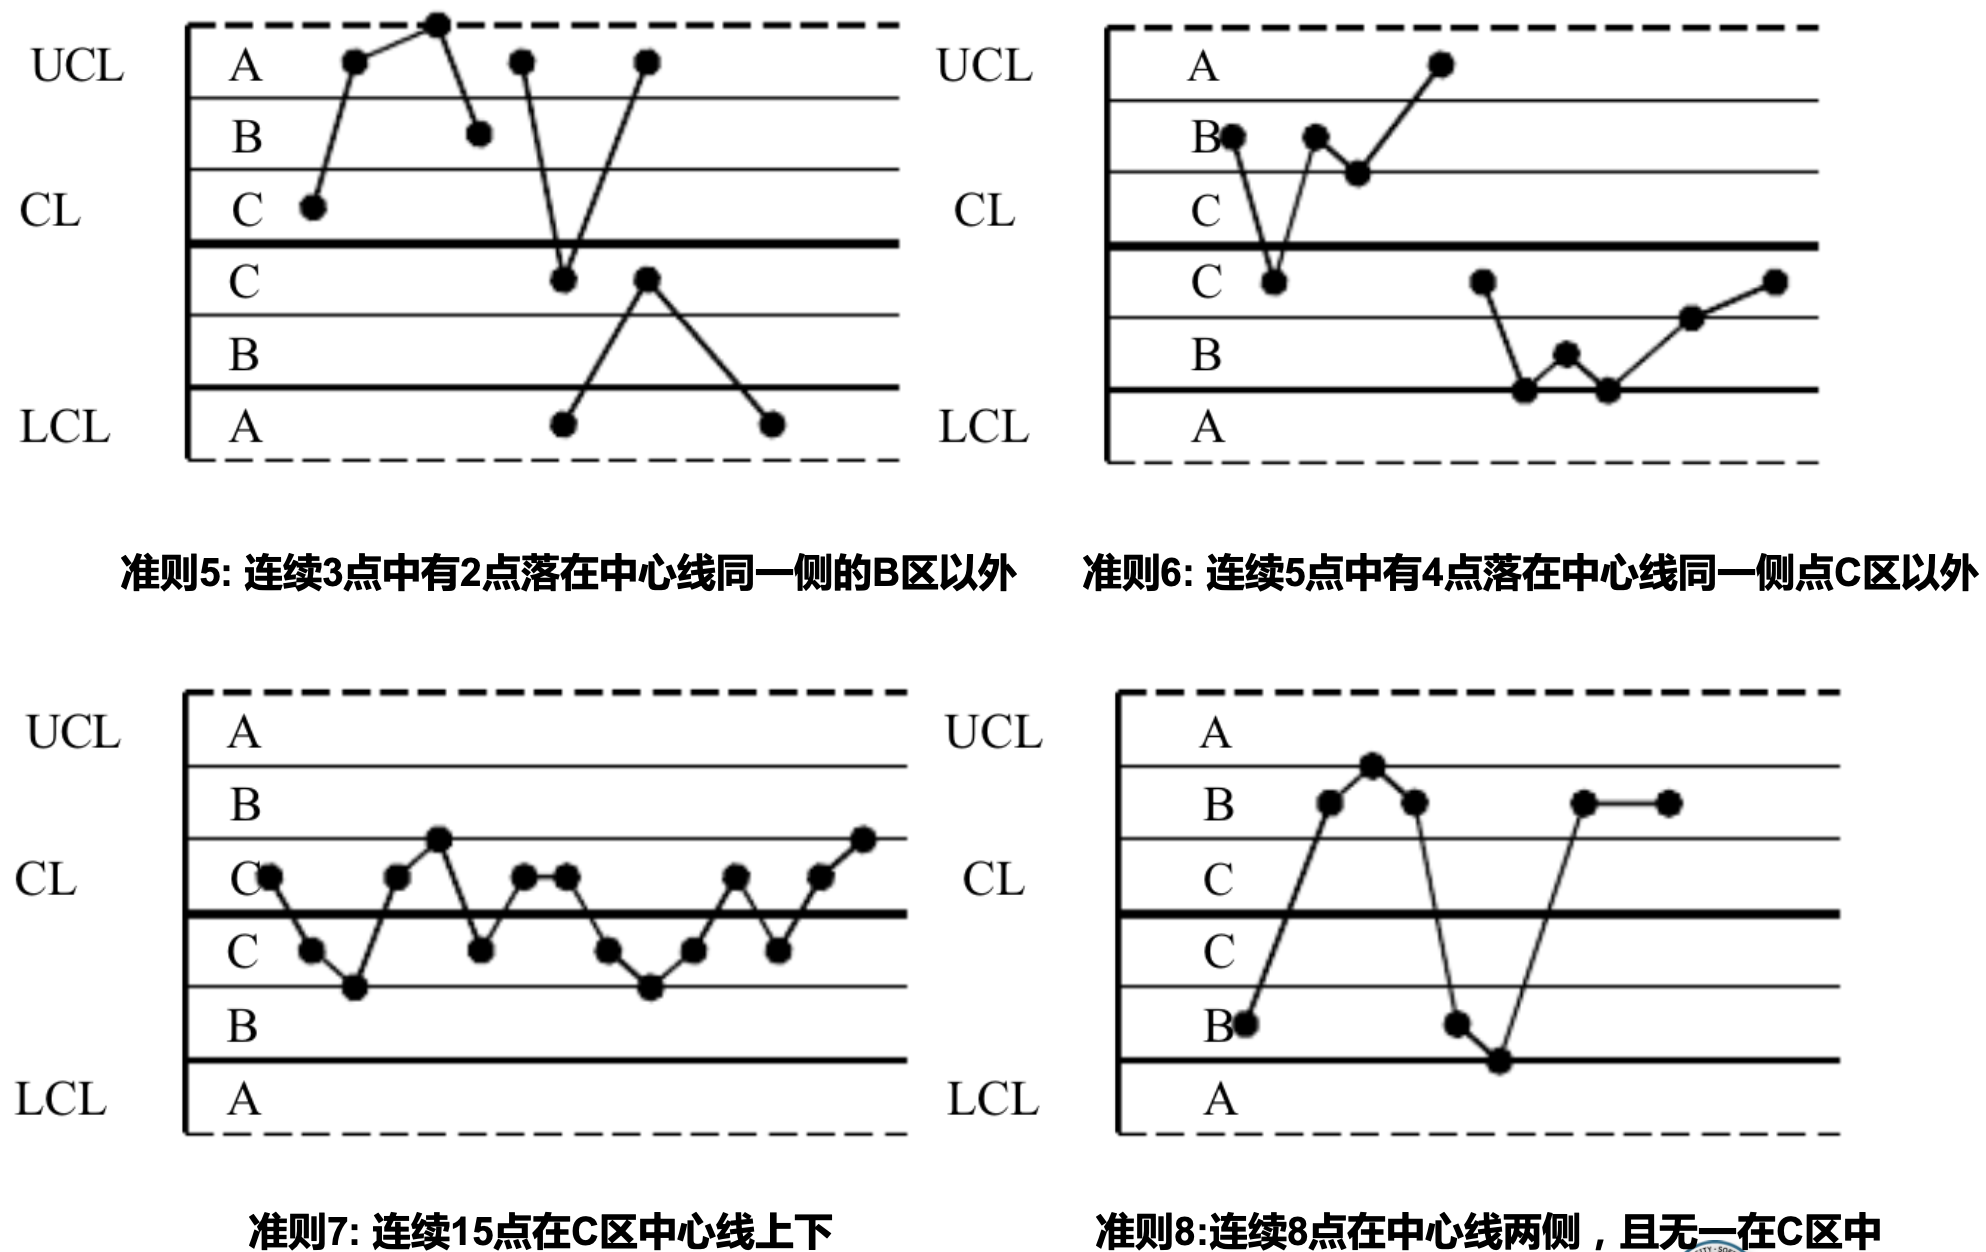
\includegraphics[width=\linewidth]{images/异常模式2.png}
	\end{minipage}
	}
	\centering
    \vspace{-1em}
\end{figure}

\begin{wraptable}{r}{0.45\textwidth}
    \centering
    \vspace{-2em}
    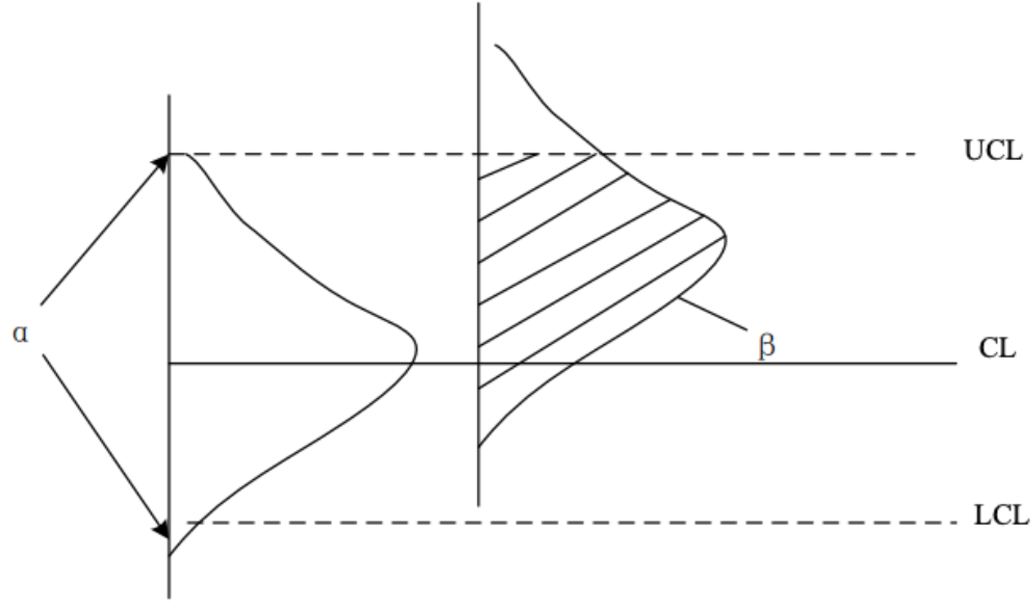
\includegraphics[width=0.45\textwidth]{images/两类错误.png}
    \vspace{-4.5em}
\end{wraptable}
两类错误(需要检验):
\begin{itemize}
    \item \uppercase\expandafter{\romannumeral1}类错误:虚发警报错误,在生产正常的情况下,纯粹出于偶然而点子出界的概率虽然很小,但不是绝对不可能发生。故当生产正常而根据点出界判断生产异常就犯了虚发警报错误,发生这种错误的概率通常记以$\alpha$。
    \item \uppercase\expandafter{\romannumeral2}类错误:漏发警报错误,在生产异常的情况下,产品质量的分布偏离典型分布,但总有一部分产品的质量特性值在上下控制界之内。如果抽到这样的产品进行检测描点,根据点未出界判断生产正常就为漏发警报错误,此概率通常记以$\beta$。
\end{itemize}

控制图典型应用流程
\begin{figure}[H]
    \vspace{-0.5em}
	\centering
	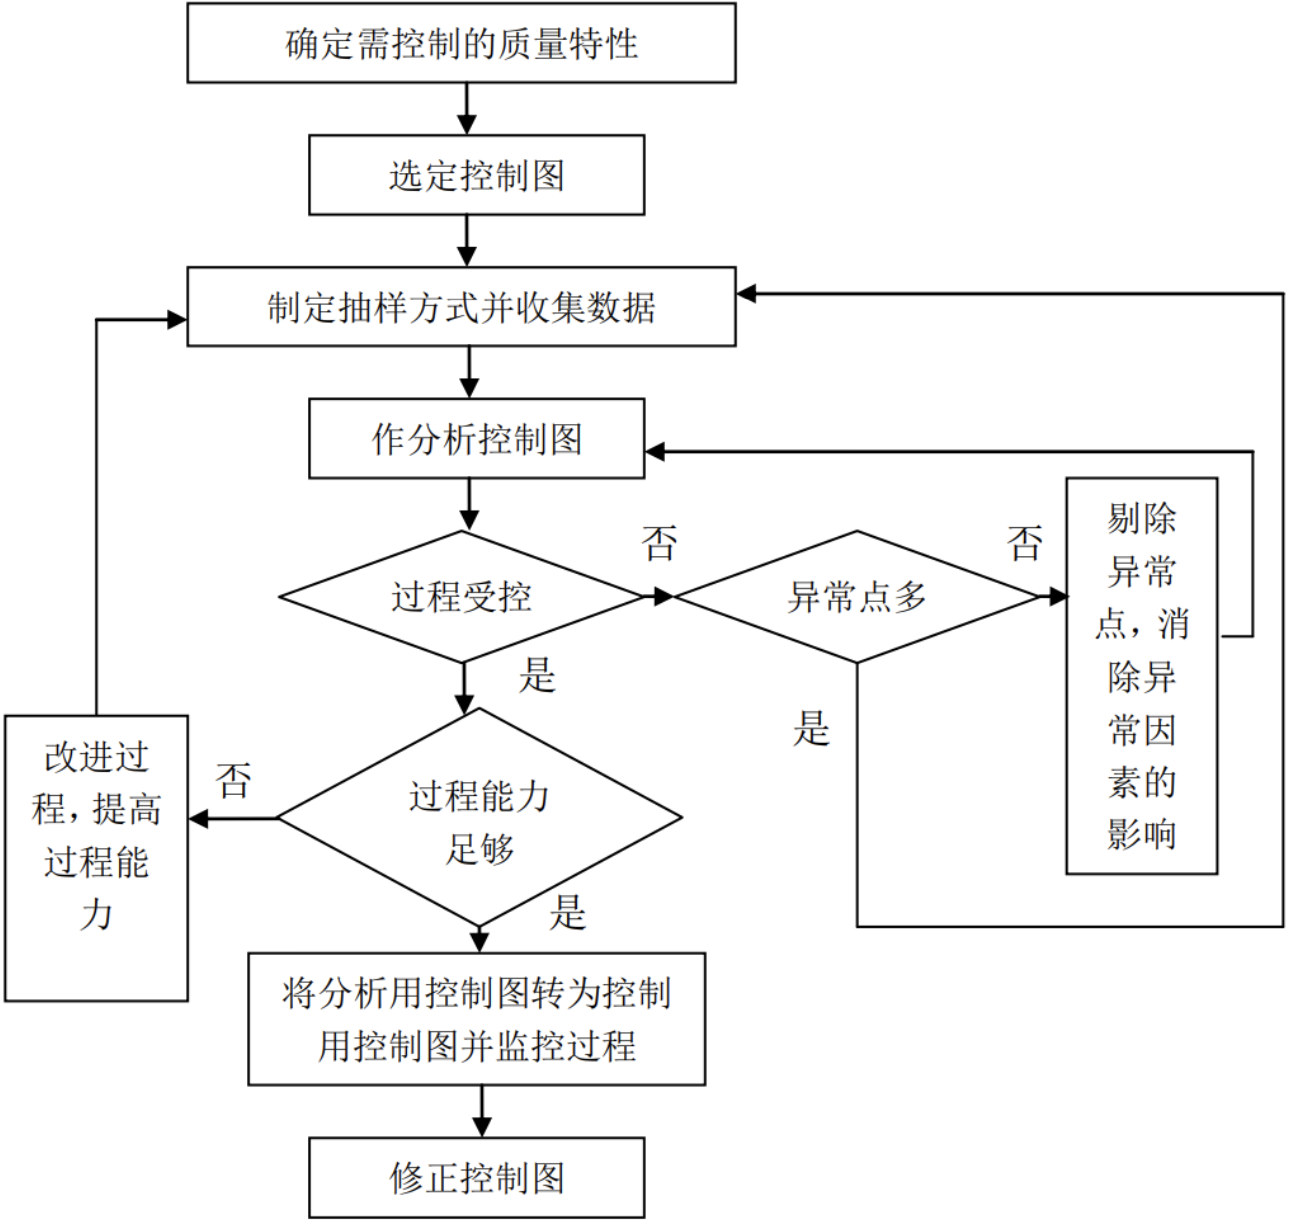
\includegraphics[width=0.6\textwidth]{images/控制图典型应用流程.png}
    \vspace{-1em}
\end{figure}

\paragraph{回归分析}~{} \par
\begin{itemize}
    \item 回归分析预测法,是在分析现象自变量和因变量之间相关关系的基础上,建立变量之间的回归方程,并将回归方程作为预测模型
    \item 回归分析预测法是一种重要的预测方法,例如,在对市场现象未来发展状况和水平进行预测时,如果能将影响市场预测对象的主要因素找到,并且能够取得其数量资料,就可以采用回归分析预测法进行预测
\end{itemize}

多变量线性回归分析步骤
\begin{figure}[H]
    \vspace{-0.5em}
	\centering
	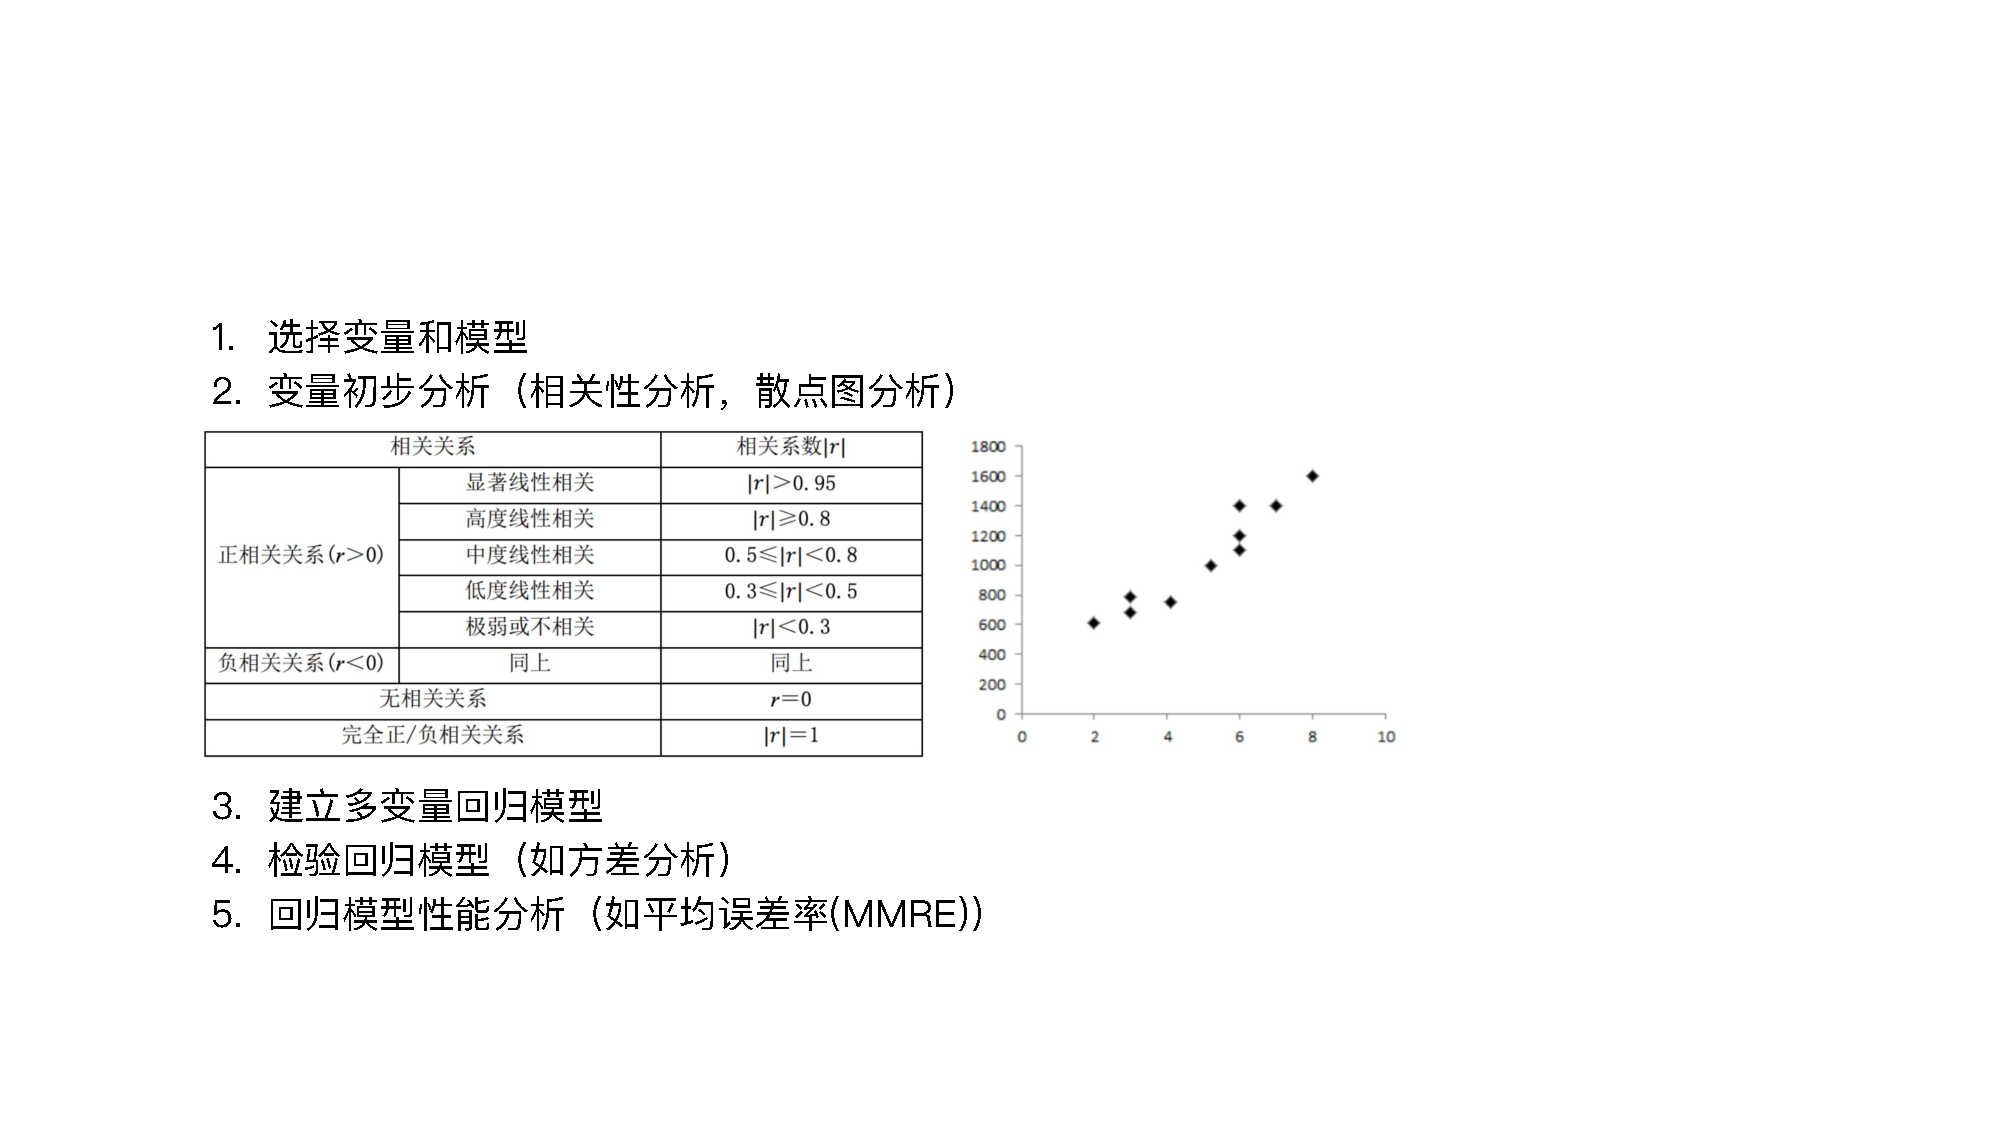
\includegraphics[width=0.65\textwidth]{images/多变量线性回归分析步骤.pdf}
    \vspace{-1em}
\end{figure}

\paragraph{假设检验}~{} \par
\begin{itemize}
    \item 假设检验又称“显著性检验”,是用来判断样本与样本,样本与总体的差异是由抽样误差引起还是本质特征差别造成的统计推断方法。其基本原理是先对总体的特征作出某种假设,然后通过抽样研究的统计推理,对此假设应该被拒绝还是接受作出推断
    \item 检验统计量:根据样本观测结果计算得到,是对样本估计量的概率标准化结果
\end{itemize}

\begin{figure}[H]
    \vspace{-0.5em}
	\centering
	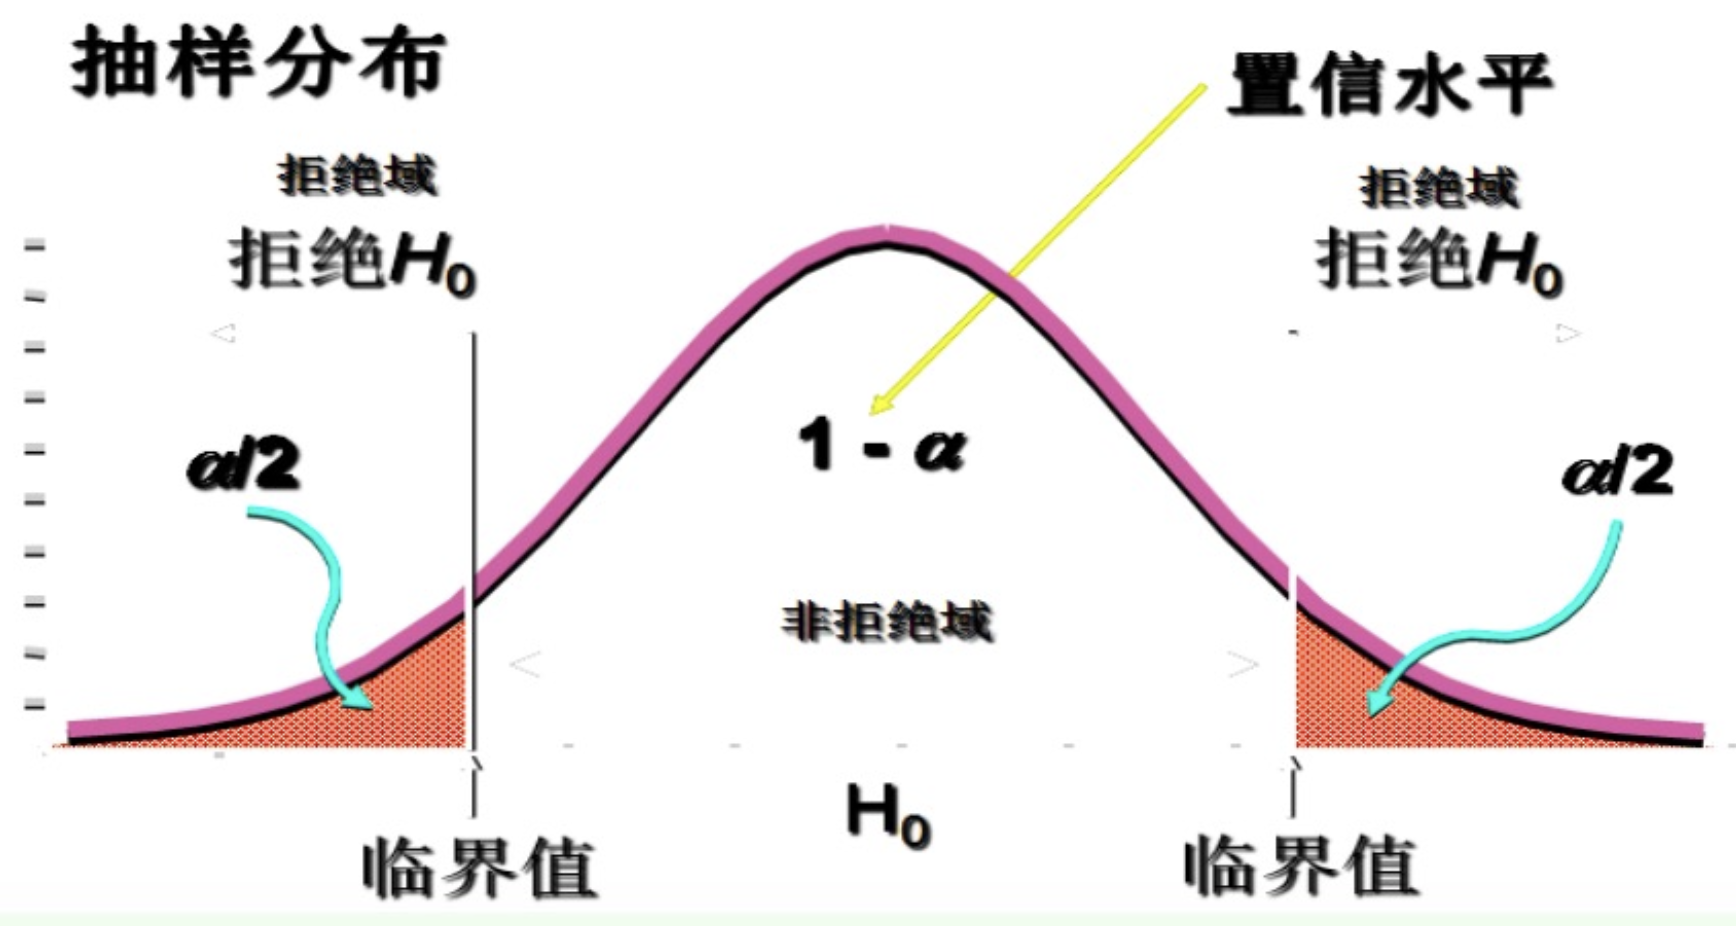
\includegraphics[width=0.45\textwidth]{images/假设检验.png}
    \vspace{-1em}
\end{figure}

假设检验步骤为:
\begin{enumerate}[label=\arabic*.]
    \item 根据问题要求建立备选假设$H_1$和原假设$H_0$(一般认为没有差异)
    \item 从研究的总体中抽出一个随机样本
    \item 选取合适的统计量,其抽样分布不含任何未知参数。利用样本数据计算具体数据。以便计算其分位点
    \item 确定一个适当的显著性水平,并计算出其临界值,指定拒绝域
    \item 将统计量的值与临界值进行比较,作出决策:
    \begin{itemize}
        \item 统计量的值落在拒绝域,拒绝$H_0$,否则不拒绝$H_0$
        \item 也可以直接利用$p$值作出决策
    \end{itemize}
\end{enumerate}

\subsubsection{方差分析}
\begin{itemize}
    \item 方差分析(ANOV):方差分析是采用数理统计的方法对所有结果进行分析,鉴别各种因素对研究对象的某些特征值影响大小的一种有效方法。用于两个及两个以上的样本均数差别的显著性检验
    \item 方差分析的目的:通过数据分析找出对该事物有显著影响的因素;研究各因素之间的交互作用是否对该事物造成影响
\end{itemize}

\subsection{仿真建模}
\subsubsection{仿真建模基本概念}
\textbf{模型:}模型是对真实或概念复杂系统的抽象。一个模型被设计用来显示人们想要研究、预测、修改或控制的系统的显著特征和特性。

\textbf{仿真模型:}仿真模型是一种计算机化的模型,代表某种动态系统或现象。当操纵真实系统的成本、风险或后勤成本过高时,这是一种获得重要见解的廉价方法。当被建模系统的复杂性超出静态模型或其他技术所能有效表示的范围时,通常采用仿真解决实际系统中经常会遇到复杂性:\textbf{系统不确定性和随机性,动态行为,反馈机制}。

\textbf{软件过程仿真模型:}软件过程仿真模型关注于特定的软件开发/维护/演化过程。它可以表示当前已实施(按现状)或计划在未来实施的过程。
\begin{itemize}
    \item 进行软件过程模型的仿真有多种原因。在许多情况下,仿真有助于决策。它还有助于降低风险,并帮助在战略、战术和运营层面进行管理。
    \item 可将使用软件过程仿真的许多原因归纳为六类目的:战略管理;规划;控制和运营管理;流程改进和技术采用;理解;培训和学习。
\end{itemize}

\subsubsection{仿真建模的步骤}
\paragraph*{确定建模的范围}~{} \par
确定模型范围是一个重要的问题,也是一个反复的过程。该模型的范围必须足够大,以完全解决提出的关键问题。

例如,公司可能正在考虑本地化到代码和单元测试步骤的过程更改。他们想开发一个模型来预测这种变化对整个项目绩效的影响。尽管对过程所做的更改仅限于代码和单元测试步骤,但更改可能会影响后期测试阶段的质量和性能。因此,模型的范围需要反映出流程变更的这些扩展影响。

\paragraph*{定义结果变量}~{} \par
结果变量是回答与模型目的一起指定的关键问题所需的信息元素。根据所提出的关键问题,可以设计出许多不同的变量作为过程模拟的结果。

典型结果变量包括以下内容:
\vspace{-0.8em}
\begin{multicols}{2}
    \begin{itemize}
        \item 成本
        \item 周期时间(又称持续时间,时间表,上市时间,间隔)
        \item 缺陷级别
        \item 随着时间的推移人员需求
        \item 人员使用率
        \item 成本/收益,投资回报率(ROI)或其他经济指标(通常对变化感兴趣)
        \item 产量/生产率
        \item 队列长度(积压)
    \end{itemize}
\end{multicols}
\vspace{-1em}

\paragraph*{过程抽象}~{} \par
在计划和开发仿真模型时,模型构建者需要确定过程的关键元素,它们之间的相互关系和行为应包括在模型中。重点应放在过程中与模型的目的特别相关并被认为会影响结果变量的那些方面。例如,要确定:
\vspace{-0.8em}
\begin{multicols}{2}
    \begin{itemize}
        \item 关键活动和任务
        \item 主要对象(例如,代码单元,设计,问题报告)
        \item 重要资源(例如人员,硬件)
        \item 活动依赖性,活动之间的对象流和排序
        \item 迭代循环,反馈循环和决策点
        \item 其他结构上的相互依赖性(例如,根据检查期间发现的缺陷数量,检查后修改 代码单元的工作)
    \end{itemize}
\end{multicols}
\vspace{-1em}

\paragraph*{选择和定义输入参数}~{} \par
要包含在模型中的输入参数(关键因素,驱动因素,独立变量)在很大程度上取决于所需的结果变量和确定的过程抽象。通常,需要许多参数来驱动软件过程仿真模型。有些需要几百个参数。下面提供了几种典型输入参数的示例:
\vspace{-0.8em}
\begin{multicols}{2}
    \begin{itemize}
        \item 收到的工作量(通常以软件大小(LOC)或功能点等衡量)
        \item 根据尺寸来进行设计的努力(Effort)
        \item 在测试或检查过程中发现缺陷的效率
        \item 代码返工的工作量取决于要纠正的缺陷的大小和数量
        \item 代码重做期间的缺陷消除和注入率
        \item 决策点结果;返工周期数
        \item 雇用率;人员流失率
        \item 随着时间的推移,人员的能力和动力
        \item 提供的培训的数量和效果
        \item 资源限制
        \item 产品版本发布的频率
    \end{itemize}
\end{multicols}
\vspace{-1em}

\begin{figure}[H]
    \vspace{-0.5em}
	\centering
	\includegraphics[width=0.55\textwidth]{images/过程仿真模型构成要素之间的关系图.png}
    \vspace{-1em}
\end{figure}

\subsubsection{常用仿真技术}
\begin{itemize}
    \item 最常用的方法:蒙特卡罗仿真、离散事件仿真和系统动力学仿真
    \item 混合仿真
\end{itemize}

\paragraph{蒙特卡罗仿真}~{} \par
蒙特卡罗方法又被称为统计模拟法或者随机抽样技术,是一种以概率和统计理论方法为基础的随机模拟方法。其原理是当要模拟的对象本身具有某种概率特征时,可以用计算机模拟的方法产生某种抽样结果,然后根据抽样结果计算统计量以及参数的值。

场景:蒙特卡洛模拟作为一种常用的模拟技术,在PMBOK里经常可以看到它的身影,其主要出现在风险管理知识领域中的定量风险分析过程,是用于做项目定量风险分析的工具之一,同时蒙特卡洛模拟也可以用于估算进度或成本以及制定进度计划等

主要步骤:
\vspace{-0.8em}
\begin{multicols}{2}
    \begin{enumerate}[label=\arabic*.]
        \item 对重要的变量建立一个概率分布
        \item 对上述的每一个变量建立起累计概率分布
        \item 为每一个变量建立随机数区间
        \item 生成随机数
        \item 进行一系列的模拟试验
    \end{enumerate}
\end{multicols}
\vspace{-1em}

\begin{wraptable}{r}{0.5\textwidth}
    \centering
    \vspace{-3em}
    \includegraphics[width=0.5\textwidth]{images/蒙特卡洛仿真示例.png}
    \vspace{-4em}
\end{wraptable}
案例:谨慎的估算师会考虑各种可能性。蒙特卡洛仿真通过为每次仿真运行从输入分布中选择随机样本,并提供概率分布作为输出来支持这种风险分析。如下是总人力的仿真结果。

\paragraph{离散事件仿真}~{} \par
\begin{wraptable}{r}{0.2\textwidth}
    \centering
    \vspace{-2em}
    \includegraphics[width=0.2\textwidth]{images/离散事件仿真主要步骤.png}
    \caption*{离散事件仿真步骤}
    \vspace{-5em}
\end{wraptable}
离散事件仿真模型是离散的和动态的,它能够使用确定的数值和各种随机数值进行蒙特卡罗仿真。离散事件仿真模型所模拟的系统的状态变量随一个个事件的发生而在特定的时间点离散变化,系统的状态变化是由(往往是随机发生的)事件驱动的。

应用场景:离散事件仿真适合于以过程为基础的场景,过程中各项活动随着事件的触发状态发生变化,具有强大的模拟各种事件流、过程流的能力,并且能够定量的评价过程能力。

离散事件系统:系统中的状态只是在离散时间点上发生变化,而这些离散时间点一般是不确定的

案例:以单服务台顾客排队为例,使用离散事件仿真模拟进行模拟。相邻两个顾客到达服务台的时间间隔服从参数为5 min的指数分布,服务员为每位顾客的服务时间服从参数为4 min的指数分布。

\begin{figure}[H]
    \vspace{-0.5em}
	\centering
	\includegraphics[width=0.35\textwidth]{images/离散事件仿真示例.png}
    \vspace{-1em}
\end{figure}

\paragraph{系统动力学仿真}~{} \par
系统动力学仿真模拟的系统的状态随时间连续变化,也称为连续仿真。它动态的使用一组不同的方程计算系统或过程随着时间的变化的趋势

场景:系统动力学仿真本质上不是随机的,和离散事件仿真相比,它主要用于从比较高阶的层面对过程进行建模,没有关注太多的细节。系统动力学仿真工具通常在过程循环方面具有很好的图形表现能力

其开发目的是为复杂的连续系统建模,以改善管理政策和组织结构

系统动力学在解决问题时主要分为以下五个具体步骤:
\begin{enumerate}[label=\arabic*.]
    \item 分析阶段:运用系统动力学方法来分析研究对象,了解系统的整体结构和系统变量之间的相互作用,来解答研究的问题
    \item 反馈机制分析阶段:首先划分系统的层次结构,了解系统整体和局部的反馈机制,确定变量的类型及变量之间的相互作用,从而明确模型的主回路
    \item 建立方程式:列出各变量规范的数学方程式,并赋予常数、表函数等相关变量的初始值
    \item 仿真模拟与政策分析:运行建立好的系统动力学模型,利用案例模拟仿真,并结合研究领域进行政策分析,进一步修改和完善系统
    \item 模型的检验和评估:利用其他一些案例资料,对该模型进行检验模拟,然后根据结果对模型进行评价
\end{enumerate}

案例:某项目的规模估计为50000 KLOC,发人员的原始数量为30,项目工期估计为450天。到目前为止已经完成了7500 KLOC,每人每天可以完成2.5 KLOC。按照这样的速度,到截止日期将有8750 KLOC未完成。以下通过系统动力学仿真模拟增加人力和加班时间对项目完成程度的影响。
\begin{figure}[H]
    \vspace{-0.5em}
	\centering
	\includegraphics[width=0.85\textwidth]{images/系统动力学仿真示例.png}
    \vspace{-1em}
\end{figure}

\paragraph{混合仿真}~{} \par
混合仿真模型指的是混合了两种或多种仿真方法的模型。在软件过程仿真方面,混合仿真通常是混合离散事件仿真和系统动力学仿真两种方法。

由于能够支持混合仿真的工具不是很多,再加上混合仿真的复杂度很高,因此混合仿真模型应用不是很广泛。

混合仿真模型既包含动态性,又包含随机性,能仿真过程循环、过程流、工作产品和资源。

\textbf{垂直分层机制:}基于垂直分层机制的软件过程混合仿真建模中,位于较高层抽象层次的仿真范式主要负责战略决策或环境动态因素的建模,而位于低层次的仿真范式主要用于构建操作层或具体实现活动(编码、集成、测试等)的仿真模型。

\textbf{水平联动机制:}该机制中不同仿真范式间没有明显的界限,不同的建模范式间是混合在一起的。迭代式软件开发过程可以采用此混合机制来建立混合仿真模型。
	\section{零散题目}
\begin{problem}
    为了制定Schedule plan,下述描述中,哪一项是不需要的:
    \uline{A}
    \vspace{-0.8em}
    \begin{multicols}{2}
        \begin{enumerate}[label=\Alph*.]
            \item Task size
            \item Task Order
            \item Schedule Hour
            \item Task hour for each task
        \end{enumerate}
    \end{multicols}
    \vspace{-1em}
\end{problem}

\begin{problem}
    在上题中,还需要补充下述哪一项数据就可以定义Schedule Plan了?
    \uline{A}
    \vspace{-0.8em}
    \begin{multicols}{4}
        \begin{enumerate}[label=\Alph*.]
            \item Task List
            \item Plan Value
            \item Earned Value
            \item Nothing
        \end{enumerate}
    \end{multicols}
    \vspace{-1em}
\end{problem}

\begin{problem}
    下列术语描述的技术或者方法是同类型的是?
    \uline{CD}    {\kaishu A. SPICE是软件过程管理;B. IDEAL是软件过程改进,XP和SCRUM是软件过程;C. 都是软件过程;D. 都是软件实践}
    \vspace{-0.8em}
    \begin{multicols}{2}
        \begin{enumerate}[label=\Alph*.]
            \item CMMI SPICE PDCA
            \item IDEAL XP SCRUM
            \item Cleanroom Gate TSP
            \item Waterfall SCRUM XP
        \end{enumerate}
    \end{multicols}
    \vspace{-1em}
\end{problem}

\begin{problem}
    请列出Capture-recapture方法进行缺陷预测的假设条件和相应的模型定义。

    常见CRC模型定义了两个参数,即评审者发现缺陷能力$t$和缺陷的难度$h$,$t$是否一致以及$h$是否一致都会影响模型。一般来说,定义如下4个基本模型:
    \vspace{-0.8em}
    \begin{multicols}{2}
        \begin{itemize}
            \item 假设$h$和$t$都一样的M0模型
            \item 假设$h$不等而$t$都一样的Mh模型
            \item 假设$t$不等而$h$都一样的Mt模型
            \item 假设$t$和$h$都不等的Mth模型
        \end{itemize}
    \end{multicols}
    \vspace{-1em}
\end{problem}

\begin{problem}
估算与计划的差异

\vspace{-0.8em}
\begin{multicols}{2}
    \begin{itemize}
        \item 估算主要用来估算待开发程序的规模和所需资源
        \item 质量计划用于保证项目的质量
        \item 包含的活动不同等等
    \end{itemize}
\end{multicols}
\vspace{-1em}
\end{problem}

\end{document}


% \begin{figure}[H]
%     \vspace{-0.5em}
% 	\centering
% 	\includegraphics[width=0.4\textwidth]{images/}
%     \vspace{-1em}
% \end{figure}


% \vspace{-0.8em}
% \begin{multicols}{2}
%     \begin{itemize}
%         \item 
%     \end{itemize}
% \end{multicols}
% \vspace{-1em}


% \vspace{-0.5em}
% \begin{spacing}{1.2}
%     \centering
%     \begin{longtable}{|W{c}{2.5cm}|W{c}{3.8cm}|W{c}{4.2cm}|m{4cm}<{\centering}|}
% 		表格内容
% 		表头居中方式  \multicolumn{1}{c|}{表头内容} 
%     \end{longtable}
% 	\end{spacing}
% \vspace{-1em}


% \begin{figure}[H]
% 	\setcounter{subfigure}{0}
% 	\centering
% 	\vspace{-0.5em}	
% 	\subfloat{
% 	\begin{minipage}[t]{0.47\linewidth}
% 	\centering
% 	\includegraphics[width=\linewidth]{}
% 	\end{minipage}
% 	}
% 	\subfloat{
% 	\begin{minipage}[t]{0.47\linewidth}
% 	\centering
% 	\includegraphics[width=\linewidth]{}
% 	\end{minipage}
% 	}
% 	\centering
% 	\vspace{-1em}
% \end{figure}


% \begin{wraptable}{r}{6.5cm}
%     \centering
%     \vspace{-1.5em}
%     \begin{tabular}{|c|c|}
%     \hline
%     期望的确定性 & 确定性因子 \\ \hline
%     95\% & 1.960  \\ \hline
%     90\% & 1.645  \\ \hline
%     85\% & 1.281  \\ \hline
%     \end{tabular}
%     \caption*{常见的确定性因子}
%     \vspace{-1.5em}
% \end{wraptable}
% 下面必须紧跟浮动体


% \vspace{-0.5em}
% \begin{shaded}

% \end{shaded}
% \vspace{-1em}


% 设定尺寸单位
% \setlength{\TPHorizModule}{\textwidth}
% \setlength{\TPVertModule}{\textwidth}

% \begin{textblock}{0.4}(0.85,1)

% \end{textblock}
